% !TEX program = pdflatexmk
% !TEX parameter = --shell-escape --lualatex

% Compilation of this document requires multiple runs of pdflatex and biber. This is
% best done automaticaly using latexmk. TiKz externalization requires shell-escape to
% be enabled.

\documentclass[
a4paper, % Page size
fontsize=10pt, % Base font size
twoside=true, % Use different layouts for even and odd pages (in particular, if twoside=true, the margin column will be always on the outside)
%open=any, % If twoside=true, uncomment this to force new chapters to start on any page, not only on right (odd) pages
%chapterentrydots=true, % Uncomment to output dots from the chapter name to the page number in the table of contents
numbers=noenddot, % Comment to output dots after chapter numbers; the most common values for this option are: enddot, noenddot and auto (see the KOMAScript documentation for an in-depth explanation)
fontmethod=tex, % Can also use "modern" with XeLaTeX or LuaTex; "tex" is the default for PdfLaTex, and "modern" is the default for those two.
% The fonts for "modern" don't seem to be included in my TeX distribution, are they Windows-only?
]{kaobook}

%----------------------------------------------------------------------------------------
%	PACKAGES AND OTHER DOCUMENT CONFIGURATIONS
%----------------------------------------------------------------------------------------

% Choose the language
\ifxetexorluatex
\usepackage{polyglossia}
\setmainlanguage{english}
\else
\usepackage[english]{babel} % Load characters and hyphenation
\fi
\usepackage[english=british]{csquotes}	% English quotes

% Load packages for testing
\usepackage{blindtext}
\usepackage{adjustbox}

\usepackage{pifont}% http://ctan.org/pkg/pifont
\newcommand{\cmark}{\ding{51}}%
\newcommand{\xmark}{\ding{55}}%
\usepackage{longtable}
\usepackage{booktabs}
\usepackage{tabularx}
\usepackage{siunitx}
\sisetup{
   separate-uncertainty
}
\usepackage{physics}

% Plots and graphs
\usepackage{pgfplots}
\usepackage{pgfplotstable}
\ifxetexorluatex
    % do nothing
\else
    \DeclareUnicodeCharacter{2212}{−}
\fi
\usepgfplotslibrary{groupplots,dateplot}
\usetikzlibrary{patterns,shapes,arrows}
\usetikzlibrary{fadings}
\pgfplotsset{compat=newest}
\usepgfplotslibrary{fillbetween}

\usepackage[compat=1.1.0]{tikz-feynman}
%\tikzfeynmanset{warn luatex=false}

% global color definitions
\definecolor{black}{RGB}{0,0,0}
\definecolor{orange}{RGB}{230, 159, 0}
\definecolor{skyblue}{RGB}{86, 180, 233}
\definecolor{bluishgreen}{RGB}{0, 158, 115}
\definecolor{yellow}{RGB}{240, 228, 66}
\definecolor{blue}{RGB}{0, 114, 178}
\definecolor{vermilion}{RGB}{213, 94, 0}
\definecolor{reddishpurple}{RGB}{204, 121, 167}

\definecolor{lightgray204}{RGB}{204,204,204}

\tikzstyle{nue_color}=[orange]
\tikzstyle{numu_color}=[bluishgreen]
\tikzstyle{nutau_color}=[skyblue]
% color for any "all NC" plots
\tikzstyle{nc_color}=[reddishpurple]
\tikzstyle{noise_color}=[blue]
\tikzstyle{muon_color}=[vermilion]

% plot an error band assuming that a table has been loaded.
% Syntax: \ploterrorband[style]{column_name}{scale_factor}
% The column name and the column "column_name__err" must exist. The
% scale factor scales the entire error band at once.
\newcommand{\ploterrorband}[3][black]{
	\addplot[const plot, #1, thick] table [x=bin_edges, y expr=\thisrow{#2} * #3] from \table;
    \addplot[const plot, #1, thin, name path=err_lo, forget plot] table[x=bin_edges, y expr=(\thisrow{#2}-\thisrow{#2__err}) * #3] from \table;
    \addplot[const plot, #1, thin, name path=err_hi, forget plot] table[x=bin_edges, y expr=(\thisrow{#2}+\thisrow{#2__err}) * #3] from \table;
    \addplot[#1, opacity=0.5, forget plot] fill between[of = err_lo and err_hi];
}

% Plot the ratio beteween two histograms with correct error propagation.
% Syntax: \plotratioerrorband[style]{nominator column}{denominator column}
% If the two columns are "x" and "y", then the ratio is x/y and the error
% on the ratio is:
%   sigma = sqrt((x * y__err)^2 + (y * x__err)^2) / y^2
% \newcommand{\plotratioerrorband}[3][black]{
% 	\addplot[const plot, #1, thick] table [x=bin_edges, y expr=\thisrow{#2} / \thisrow{#3}] from \table;

%     \addplot[const plot, #1, thin, name path=err_lo, forget plot] table[x=bin_edges,
%     y expr=
%     	\thisrow{#2} / \thisrow{#3}
% 		-
% 		sqrt(
%             (\thisrow{#2} * \thisrow{#3__err})^2 + (\thisrow{#3} * \thisrow{#2__err})^2
% 		) / \thisrow{#3}^2
% 	] from \table;

% 	\addplot[const plot, #1, thin, name path=err_hi, forget plot] table[x=bin_edges,
%     y expr=
%     	\thisrow{#2} / \thisrow{#3}
% 		+
% 		sqrt(
%             (\thisrow{#2} * \thisrow{#3__err})^2 + (\thisrow{#3} * \thisrow{#2__err})^2
% 		) / \thisrow{#3}^2
% 	] from \table;

%     \addplot[#1, opacity=0.5, forget plot] fill between[of = err_lo and err_hi];
% }

% Plot the ratio error band between two histograms, assuming that the denominator is the sum
% of the nominator and some background. This applies to any ratio where the denominator is the total MC
% and the nominator is some component. The difference w.r.t. \plotratioerrorband is that the two
% histograms are *dependent*. This reduces the error in particular for cases where the component
% for which the ratio is plotted also dominantly makes up the total.
% The error calculation is derived by expressing the ratio x / y, where x and y are dependent, as
%     f = x / (x + b),
% where now x and b are independent. The variance of b is
%     sigma_b^2 = sigma_y^2 - sigma_x^2.
% Applying the error propagation and then replacing b = y - x back into the result we find
%    sigma_f = sqrt( (y * sigma_x)^2 + (x * sigma_y)^2 - 2*x*y*sigma_y^2) / y^2
\newcommand{\plotratioerrorband}[3][black]{
	\addplot[const plot, #1, thick] table [x=bin_edges, y expr=\thisrow{#2} / \thisrow{#3}] from \table;

    \addplot[const plot, #1, thin, name path=err_lo, forget plot] table[x=bin_edges,
    y expr=
    	\thisrow{#2} / \thisrow{#3}
		-
		sqrt(
            (\thisrow{#2} * \thisrow{#3__err})^2 + (\thisrow{#3} * \thisrow{#2__err})^2 - (2 * \thisrow{#2} * \thisrow{#3} * \thisrow{#2__err}^2)
		) / \thisrow{#3}^2
	] from \table;

	\addplot[const plot, #1, thin, name path=err_hi, forget plot] table[x=bin_edges,
    y expr=
    	\thisrow{#2} / \thisrow{#3}
		+
		sqrt(
            (\thisrow{#2} * \thisrow{#3__err})^2 + (\thisrow{#3} * \thisrow{#2__err})^2 - (2 * \thisrow{#2} * \thisrow{#3} * \thisrow{#2__err}^2)
		) / \thisrow{#3}^2
	] from \table;

    \addplot[#1, opacity=0.5, forget plot] fill between[of = err_lo and err_hi];
}


\pgfplotsset{error bar legend/.style={%
    /pgfplots/legend image code/.prefix code={%
      \pgfkeysgetvalue{/pgfplots/error bars/error mark}{\pgfplotserrorbarsmark}%
      \draw[%
        /pgfplots/every error bar,
        mark=\pgfplotserrorbarsmark,
        /pgfplots/error bars/error mark options,
        sharp plot,
        ##1
      ] plot coordinates {(0.3cm, -0.1cm) (0.3cm, 0.1cm)};%
    }
  }
}

\newcommand{\ploterrorbar}[2][black]{
    \addplot[
        mark=*,
        mark options={scale=0.5, fill=black},
        #1,
        only marks,
        error bar legend,
        error bars/.cd,
        x dir=none,
        y dir=both,
        y explicit
    ] table [x=bin_midpoints, y=#2, y error=#2__err]  from \table;
}

\usepackage{helvet}
\usepackage[eulergreek]{sansmath}
\pgfplotsset{
    tick label style = {font=\footnotesize\sansmath\sffamily},
    every axis label = {font=\footnotesize\sansmath\sffamily},
    % the eulergreek style for math looks oddly different from the
    % rest of the document, so we omit \sansmath here
    label style = {font=\footnotesize\sffamily},
    % global legend style applied to all plots (set per plot to override)
    legend style = {
        font=\footnotesize\sffamily,
        fill opacity=0.8,
        draw opacity=1,
        text opacity=1,
        at={(0.5,0.95)},
        anchor=north,
        draw=lightgray204,
        % hack to get better legend spacing, see
        % https://tex.stackexchange.com/questions/18152/how-can-i-adjust-the-horizontal-spacing-between-legend-entries-in-pgfplots
        /tikz/every even column/.append style={column sep=0.1cm}
    },
    legend cell align={left}
}

\tikzstyle{plot annotation}=[
    font=\footnotesize\sffamily,
    fill opacity=0.8,
    draw opacity=1,
    text opacity=1,
    draw=lightgray204,
    fill=white
]


% Load the bibliography package
\usepackage{aas_macros}
\usepackage[giveninits=true]{kaobiblio}
\addbibresource{refs.bib} % Bibliography file

% Colors
\usepackage[dvipsnames]{xcolor}

% Load mathematical packages for theorems and related environments
\usepackage[framed=true]{kaotheorems}
\usepackage{amsmath}
\usepackage{nicefrac}
\renewcommand{\rm}{\mathrm}
% Load the package for hyperreferences
\usepackage{kaorefs}

\usepackage{caption}
\usepackage{subcaption}

\graphicspath{{./}{figures/}{tikz/}} % Paths in which to look for images

\makeindex[columns=3, title=Alphabetical Index, intoc] % Make LaTeX produce the files required to compile the index

%----------------------------------------------------------------------------------------

\newcommand{\numucc}{$\nu_{\mu,\,\rm CC}$}

% command to simplify writing total differentials
\newcommand{\drm}{\mathrm{d}}

% Make an overbar in parentheses
\newcommand{\pbar}[1]{\overset{\textbf{\fontsize{4pt}{4pt}\selectfont(---)}}{#1}}

% Reset sidenote counter at chapters
%\counterwithin*{sidenote}{chapter}

%----------------------------------------------------------------------------------------
\renewcommand{\thefootnote}{\roman{footnote}}



% For some reason this *must* be placed here, right before the start of the
% document!
% externalization to avoid repeated compilation of pgfplots
\usepgfplotslibrary{external}
% Use a sub-directory for these intermediate files. It will look empty in the
% web-interface, but if you compile locally, they will be there.
\tikzexternalize[prefix=tikz/]
% very important: ONLY do this for figures for which we have given a name!
% otherwise, there will be a bunch of tiny unnamed output PDFs and errors.
\tikzset{external/only named=true}

%%%% UN-COMMENT TO FORCE REMAKE ALL TEX FIGURES %%%%
%\tikzset{external/force remake}

\begin{document}

%----------------------------------------------------------------------------------------
\frontmatter % Denotes the start of the pre-document content, uses roman numerals

%----------------------------------------------------------------------------------------
%	BOOK INFORMATION
%----------------------------------------------------------------------------------------
\KOMAoptions{twoside=false}
\begin{titlepage}
	\begin{center}
	\vspace*{1cm}

	\LARGE
	\textbf{Search for eV-scale sterile neutrinos with IceCube DeepCore}
	\large

	\vspace{0.8cm}

	\textbf{Dissertation}\\
	zur Erlangung des akademischen Grades\\
	doctor rerum naturalium \\
	(Dr. rer. nat.) \\

	\vspace{0.5cm}

	im Fach: Physik \\
	Spezialisierung: Experimentalphysik\\

	\vspace{0.5cm}

	eingereicht an der \\
	Mathematisch-Naturwissenschaftlichen Fakultät\\
	der Humboldt-Universität zu Berlin\\

	\vspace{0.5cm}

	von\\
	\textbf{Alexander Trettin M. Sc}\\
%	\vspace{0.8cm}
	geboren am 07. Mai 1993\\
	in Kiel

	\vspace{0.5cm}

	Präsidentin der Humboldt-Universität zu Berlin\\
	Prof. Dr.-Ing. Dr. Sabine Kunst\\

	\vspace{0.5cm}

	Dekan der Mathematisch-Naturwissenschaftlichen Fakultät\\
	Prof. Dr. Elmar Kulke\\

	\end{center}
	\newpage

	\vspace*{8cm}

	\textbf{No copyright}\\
	\cczero\ This book is released into the public domain using the CC0 code. To the extent possible under law, I waive all copyright and related or neighbouring rights to this work.

	To view a copy of the CC0 code, visit: \\\url{http://creativecommons.org/publicdomain/zero/1.0/}

	\medskip

	\textbf{Colophon} \\
	This document was typeset with the help of \href{https://sourceforge.net/projects/koma-script/}{\KOMAScript} and \href{https://www.latex-project.org/}{\LaTeX} using the open-source \href{https://github.com/fmarotta/kaobook/}{kaobook} template class.\\

	% TODO: upload to GitHub, sync
	\todo[inline, noinlinepar]{Link to code }
	% The source code of this thesis is available % at:\\\url{https://github.com/robertdstein/kaobook}, \\while the scripts used to generate the % plots are available at: \\\url{https://github.com/robertdstein/thesis_code}\\

	\medskip

	\textbf{Publisher} \\
	\todo[inline, noinlinepar]{add when first printed, by whom}
	%First printed in Nov 2022 by Humboldt Universität zu Berlin

	% \newpage
	%
	% \vspace*{5.0cm}
	%
	% \large
	% A neutrino is not a big thing to be hit by. \\
	% In fact it's hard to think of anything much smaller by which one could reasonably hope to be % hit. And it's not as if being hit by neutrinos was in itself a particularly unusual event for % something the size of the Earth. Far from it. It would be an unusual nanosecond in which the % Earth was not hit by several billion passing neutrinos.\\
	% \flushright --\textit{The Hitchhiker's Guide to The Galaxy}
	%
	% \afterpage{\blankpage}

\end{titlepage}
\title[Search for eV-scale sterile neutrinos with IceCube DeepCore]



%----------------------------------------------------------------------------------------
%	COPYRIGHT PAGE
%----------------------------------------------------------------------------------------
% \makeatletter
% \uppertitleback{\@titlehead} % Header
% \lowertitleback{

% 	\textbf{No copyright}\\
% 	\cczero\ This book is released into the public domain using the CC0 code. To the extent possible under law, I waive all copyright and related or neighbouring rights to this work.

% 	To view a copy of the CC0 code, visit: \\\url{http://creativecommons.org/publicdomain/zero/1.0/}

% 	\medskip

% 	\textbf{Colophon} \\
% 	This document was typeset with the help of \href{https://sourceforge.net/projects/koma-script/}{\KOMAScript} and \href{https://www.latex-project.org/}{\LaTeX} using the open-source \href{https://github.com/fmarotta/kaobook/}{kaobook} template class.\\

% 	The source code of this thesis is available at:\\\url{https://github.com/robertdstein/kaobook}, \\while the scripts used to generate the plots is available at: \\\url{https://github.com/robertdstein/thesis_code}\\

% 	\medskip

% 	\textbf{Publisher} \\
% 	First printed in Nov 2021 by Humboldt Universität zu Berlin
% }
% \makeatother
%----------------------------------------------------------------------------------------
%	DEDICATION
%----------------------------------------------------------------------------------------
% \dedication{
% 	A neutrino is not a big thing to be hit by. \\

% 	In fact it's hard to think of anything much smaller by which one could reasonably hope to be hit. And it's not as if being hit by neutrinos was in itself a particularly unusual event for something the size of the Earth. Far from it. It would be an unusual nanosecond in which the Earth was not hit by several billion passing neutrinos.\\
% 	\flushright --\textit{The Hitchhiker's Guide to The Galaxy}
% }
%----------------------------------------------------------------------------------------
%	OUTPUT TITLE PAGE AND PREVIOUS
%----------------------------------------------------------------------------------------
% Note that \maketitle outputs the pages before here
% If twoside=false, \uppertitleback and \lowertitleback are not printed
% To overcome this issue, we set twoside=semi just before printing the title pages, and set it back to false just after the title pages
\KOMAoptions{twoside=semi}
\KOMAoptions{twoside=false}
%----------------------------------------------------------------------------------------
%	PREFACE
%----------------------------------------------------------------------------------------
%\chapter*{Preface}
\addcontentsline{toc}{chapter}{Preface} % Add the preface to the table of contents as a chapter

I am of the opinion that every \LaTeX\xspace geek, at least once during 
his life, feels the need to create his or her own class: this is what 
happened to me and here is the result, which, however, should be seen as 
a work still in progress.
Actually, this class is not completely 
original, but it is a blend of all the best ideas that I have found in a 
number of guides, tutorials, blogs and tex.stackexchange.com posts.
In 
particular, the main ideas come from two sources:

\begin{itemize}
	\item \href{https://3d.bk.tudelft.nl/ken/en/}{Ken Arroyo Ohori}'s 
	\href{https://3d.bk.tudelft.nl/ken/en/nl/ken/en/2016/04/17/a-1.5-column-layout-in-latex.html}{Doctoral 
	Thesis}, which served, with the author's permission, as a backbone 
	for the implementation of this class;
	\item The 
		\href{https://github.com/Tufte-LaTeX/tufte-latex}{Tufte-Latex 
			Class}, which was a model for the style.
\end{itemize}

The first chapter of this book is introductory and covers the most
essential features of the class.
Next, there is a bunch of chapters 
devoted to all the commands and environments that you may use in writing 
a book; in particular, it will be explained how to add notes, figures 
and tables, and references.
The second part deals with the page layout 
and design, as well as additional features like coloured boxes and 
theorem environments.

I started writing this class as an experiment, and as such it should be 
regarded.
Since it has always been intended for my personal use, it may
not be perfect but I find it quite satisfactory for the use I want to 
make of it.
I share this work in the hope that someone might find here 
the inspiration for writing his or her own class.

\begin{flushright}
	\textit{Federico Marotta}
\end{flushright}

%\index{preface}
\chapter{Abstract}

Here be the abstract.\todo{write abstract}

\cleardoubleoddpage
\chapter{Zusammenfassung}

Eine Zusammenfassung sollte ebenfalls auf Deutsch geschrieben werden.
Wenn du jemals dachtest, du seist nutzlos, so denke daran, dass es diese Zusammenfassungen gibt.
\cleardoubleoddpage
%----------------------------------------------------------------------------------------
%	TABLE OF CONTENTS & LIST OF FIGURES/TABLES
%----------------------------------------------------------------------------------------
\begingroup % Local scope for the following commands
% Define the style for the TOC, LOF, and LOT
%\setstretch{1} % Uncomment to modify line spacing in the ToC
%\hypersetup{linkcolor=olive} % Uncomment to set the colour of links in the ToC
\setlength{\textheight}{230\hscale} % Manually adjust the height of the ToC pages
% Turn on compatibility mode for the etoc package
\etocstandarddisplaystyle % "toc display" as if etoc was not loaded
\etocstandardlines % "toc lines as if etoc was not loaded
\tableofcontents % Output the table of contents
\listoffigures % Output the list of figures
% Comment both of the following lines to have the LOF and the LOT on different pages
%\let\cleardoublepage\bigskip
%\let\clearpage\bigskip
\listoftables % Output the list of tables

\listoftodos

\endgroup
%----------------------------------------------------------------------------------------
%	MAIN BODY
%----------------------------------------------------------------------------------------
\mainmatter % Denotes the start of the main document content, resets page numbering and uses arabic numbers
\setchapterstyle{kao} % Choose the default chapter heading style

\setchapterstyle{kao}
\setchapterpreamble[u]{\margintoc}
\chapter{Introduction}
\labch{intro}

The neutrino is a nearly massless and electrically neutral particle whose existence was first conjectured by Pauli in the 1930s to explain the fact that the energy spectrum of radiation from nuclear beta decay was continuous. If the only particles produced by the decay were the nucleus and the beta particle, then the energy of the beta particle would have been fixed by conservation of energy and momentum. It was a bold proposition at the time, because there were no observable traces of this particle and Pauli himself feared that it might be unobservable. His fears proved unwarranted when the first direct experimental observation of neutrinos was made in 1956 by Cowan and Reines\cite{cowan:1956} by detecting the distinct signature of so-called "inverse" beta-decay reaction
\begin{equation}
    \bar{\nu} + p \rightarrow n + e^+
\end{equation}
inside a water tank close to a nuclear reactor. About a decade later, in 1960, the Homestake experiment was able to measure the flux of neutrinos from the Sun. However, the observed rate of electron neutrinos was lower than what was expected from nuclear fusion reactions inside the Sun, leading to the \emph{solar neutrino problem}. The muon neutrino was discovered in 1962 by an experiment at the Brookhaven National Laboratory\cite{PhysRevLett.9.36} and the tau neutrino in 2000 by the DONUT experiment at Fermilab\cite{Kodama_2001}, completing the current picture of the Standard Model (SM) with three generations of leptons. In this model, neutrinos are described as spin-$\nicefrac{1}{2}$ fermions that only interact via the Weak nuclear force. The Weak force only interacts with left-handed chiral neutrinos and right-handed chiral antineutrinos, and no other neutrino states have so far been observed. This description requires that neutrinos are massless, because the Higgs mechanism that produces the masses of all other particles in the SM requires an interaction involving both right-handed and left-handed chiral fields.

The solution to the solar neutrino problem accepted today is that neutrinos have the ability to oscillate from one flavor to another. In this way, the electron neutrinos that are initially produced by the Sun can turn into a different flavor to which the Homestake experiment was not sensitive. This phenomenon of \emph{neutrino oscillations} was first demonstrated by the Super-Kamiokande experiment for muon neutrinos that are produced in the Earth's atmosphere\cite{PhysRevLett.81.1562}. In 2002, the SNO experiment provided the first direct evidence that this flavor conversion was also happening to electron neutrinos from the Sun\cite{PhysRevLett.89.011301}. The existence of neutrinos oscillations has profound implications, because it means that neutrinos cannot be massless.

Neutrino oscillations can be explained by postulating that the flavor eigenstates with which the Weak force interacts are mixtures of different mass eigenstates. The mass eigenstates can be described as wave packets with slightly different frequencies that overlap. These wave packets travel at different speeds due to their mass differences and therefore interfere with one another, leading to the phenomenon of neutrino oscillations. However, the SM provides no explanation of how neutrinos acquire their masses. The Higgs mechanism requires couplings of both left-handed and right-handed chiral fields to the Higgs field, but there are no right-handed neutrinos in the SM. The extreme lightness of the neutrinos compared to other particles suggests that the process that produces them might be different altogether from the process that generates the masses of all other particles. Neutrino oscillations, therefore, are direct evidence of physics beyond the Standard Model (BSM) and motivate the search for new particles and forces that might be involved in the process of neutrino mass genereration.

This work describes a neutrino oscillation measurement using the IceCube Neutrino Observatory, a neutrino detector located at the geographic South Pole. It uses 5160 optical sensors deployed in a volume of one cubic kilometer of the Antarctic glacier to measure faint flashes of Cherenkov light that is produced when neutrinos interact with the ice. It can detect neutrinos in a wide energy range starting from atmospheric neutrinos at a few GeV up to the PeV energy range of cosmic neutrinos. The data analysis presented in this work uses observations from the DeepCore sub-array of IceCube that is specifically optimized for the detection of neutrinos that are produced in the atmosphere of the Earth. These neutrinos consist mostly of muon neutrinos that travel through the Earth and have a chance to oscillate into other neutrino flavors before they are detected at the South Pole. After collecting tens of thousands of neutrinos over the course of several years, the muon neutrino survival probability can be estimated to a high precision. The results allow inferences about the mass differences between different neutrino states and can be probed for signs of BSM physics.

\Cref{ch:stdmodel} of this thesis summarizes how neutrinos are described in the Standard Model. A particular emphasis of this chapter is the famous Higgs mechanism by which all particles in the SM acquire their mass and how this mechanism can be expanded to include neutrino masses. In \refch{massoscillations}, we will describe how the mass differences between neutrinos lead to neutrino oscillations and how these oscillations manifest in experimental observations. The chapter also describes the experimental anomalies of neutrino oscillation measurements that motivate the search for additional heavy neutrino states of the eV scale. The IceCube Neutrino Observatory is introduced in \refch{icecube} with special focus on the DeepCore sub-array. The chapter will also describe in detail how the DeepCore data is filtered to produce a data sample with a high purity of muon neutrinos. The data sample is then used for two different measurements: The first, described in \refch{measurement-three-flavor}, measures the parameters that characterize the muon neutrino survival probability in the picture of three oscillating neutrino flavors. The second measurement, shown in \refch{measurement-sterile}, is probing the observed oscillation pattern for signs of an additional heavier neutrino mass eigenstate that is associated with an otherwise non-interacting \emph{sterile} neutrino. The result of this measurement places limits on the amount of mixing that is allowed between the hypothetical sterile neutrino state and the three known active neutrino flavors. With these constraints, this work provides another puzzle piece in the search for the origin of neutrino masses.



\setchapterpreamble[u]{\margintoc}
\setchapterstyle{kao}
% \setchapterimage[6.5cm]{figures/artwork/Alexander_Trettin_illustrations_of_wave_functions_and_particle__21cc39d2-0bda-4230-9b29-9bfd8707df01.png}
\chapter{Neutrinos in the Standard Model}

\labch{stdmodel}

The Standard Model (SM) of particle physics is a relativistic quantum field theory based on the gauge symmetry group $\mathrm{SU}(3)_C \times \mathrm{SU}(2)_L \times \mathrm{U}(1)_Y$, where the sub-scripts $C$, $L$ and $Y$ correspond to the conserved quantities \emph{color}, \emph{left-handed chirality} and \emph{weak hypercharge}, respectively. In this model, all matter particles are described as fermions, that is, excitations of Dirac-type fermion fields permeating space-time. The forces acting between fermions are mediated by an exchange of bosons, and all interactions must preserve the over-all symmetry of the theory. Since its completion in the early 1970s, it has been shown to an impressive degree of precision that it accurately describes the interactions between elementary particles due to the Strong Force, the Weak Force and the electromagnetic force. It can also explain how quarks and leptons acquire their masses via the Higgs mechanism, whose by-product, the Higgs boson, was detected at the LHC in 2012\todo{cite Higgs discovery}. Despite its success, the Standard Model has some known shortcomings such as its incompatibility with General Relativity and inability to explain cosmological phenomena most commonly interpreted as Dark Matter and Dark Energy.  Most relevantly for this work, it predicts that neutrinos should be massless and therefore does not allow for neutrino oscillations. Since neutrino oscillations can be experimentally observed at very high statistical significance\todo{cite nobel prize SuperK}, it is clear that the SM has to be extended in such a way that neutrino masses can be accommodated. There are several candidate theories for such an extension, but none of them could so far be confirmed experimentally. This chapter will first describe the properties and interactions of neutrinos as they are described by the SM. Then, it will show the mathematical formulation of neutrino oscillations, and finally it will describe some of the simplest extensions to the SM that could explain how neutrinos acquire their mass.

\section{Standard Model particles}

The elementary particles of the SM are organized into fermions and bosons, where fermions make up the observable matter while bosons are the particles that mediate forces. The number of force-mediating bosons is determined by the generators of the symmetry groups that all interactions must obey, while the strength of each force is determined by a \emph{coupling constant} that has to be estimated experimentally. There are eight massless gluons that correspond to the generators of the $\mathrm{SU}(3)_C$ group and mediate the Strong force. All Strong interactions conserve the so-called \emph{color} charge of the involved particles. The symmetry group $\mathrm{SU}(2)_L \times \mathrm{U}(1)_Y$ is the combined symmetry of the \emph{electroweak} force and produces the gauge boson fields $W_1$, $W_2$, $W_3$ and $B$. The electroweak symmetry group is broken into the $\mathrm{U}(1)_Q$ group by interactions of fermions with the Higgs field (further described below) that mixes the $W$ and $B$ fields into massive $W^\pm$ and $Z^0$ bosons and a massless photon $\gamma$ such that
\begin{align}
    Z &= \cos \theta_W W_3 - \sin \theta_W B \\
    \gamma &= \sin \theta_W W_3 + \cos \theta_W B\\
    W^\pm &= \frac{1}{\sqrt{2}} (W_1 \mp iW_2)\;,\label{eq:ew-boson-definitions}
\end{align}
where $\theta_W$ is the so-called \emph{Weinberg angle}.
\begin{margintable}
    \caption{Fermions in the Standard Model}
    \label{tab:fermions-sm}
    \centering
    \begin{tabular}{ccccc} \toprule
    & \multicolumn{3}{c}{generation} & \\ \cmidrule{2-4}
    & 1 & 2 & 3 & charge \\ \midrule
    \multirow{4}{*}{\rotatebox[origin=c]{90}{quarks}}\\
    & u & c & t & $+\nicefrac{2}{3}$ \\
    & d & s & b & $-\nicefrac{1}{3}$ \\
    \\ \midrule
    \multirow{4}{*}{\rotatebox[origin=c]{90}{leptons}}\\
    & $\nu_e$ & $\nu_\mu$ & $\nu_\tau$ & 0 \\
    & $e$ & $\mu$ & $\tau$ & $-1$ \\
    \\ \bottomrule
    \end{tabular}
\end{margintable}
The fermions of the SM are divided into quarks and leptons. Quarks participate in all strong, weak and electromagnetic interactions and are always found in combinations that form baryons (protons, neutrons) or mesons (kaons, pions). The leptons, on the other hand, do not participate in strong interactions. Charged leptons are massive and participate in both the weak and the electromagnetic force, while neutral leptons, the neutrinos, are massless and participate only in weak interactions. All fermions can be grouped into three \emph{generations} of quarks and leptons that are only distinguished by their masses, leading to a convenient arrangement of quarks and leptons into a $3\times4$ scheme as shown in \reftab{fermions-sm}.

\subsection{Electroweak Symmetry Breaking}
\labsec{ew-symmetry-breaking}
The process of breaking the $\mathrm{SU}(2)_L \times \mathrm{U}(1)_Y$ symmetry group deserves special attention for the purposes of this work, because it is the process by which the exchange bosons of the Weak force acquire their mass. If the symmetry was unbroken, as it is the case for the $\mathrm{SU(3)}$ group of the Strong force, then the exchange bosons would all remain massless, just like the gluons. To simplify the discussion, the process can be illustrated using only the first generation of SM fermions. The starting point is to introduce the Higgs doublet of complex scalar fields
\begin{equation}
    \Phi = \begin{pmatrix}
        \Phi^+ \\
        \Phi^0
    \end{pmatrix}\;,\label{eq:higgs-doublet}
\end{equation}
where $\Phi^+$ is charged and $\Phi^0$ is neutral\sidenote{In a more general discussion, the Higgs doublet would be written down without assigning the charges a priori, they would be derived later. See \cite{schwartz_2013} for a more rigorous derivation.}. The Lagrangian describing the dynamics of this field,
\begin{equation}
    \mathcal{L}_\mathrm{Higgs} = (D_\mu \Phi^\dag)(D^\mu \Phi) - \lambda \left( \Phi^\dag \Phi - \frac{v^2}{2} \right)^2\;,\label{eq:higgs-lagrangian}
\end{equation}
with the covariant derivative
\begin{equation}
    D_\mu \Phi= \partial_\mu \Phi - ig W_\mu^a \tau^a \Phi - \frac{1}{2}ig'B_\mu \Phi
\end{equation}
is invariant under $\mathrm{SU}(2)_L \times \mathrm{U}(1)_Y$ symmetry and adds a quartic self-interaction potential with the parameters $\lambda$ and $v$, where $\lambda$ is taken to be positive, such that the potential is bounded from below. The fields $W_\mu^a$ in the covariant derivative correspond to the gauge bosons of the $\mathrm{SU}(2)_L$ group whose generators are $\tau^a = \frac{\sigma^a}{2}$, where $\sigma^a$ are the Pauli matrices. The $B_\mu$ field is the boson of the $\mathrm{U}(1)_Y$ group. The factors $g$ and $g'$ are the $\mathrm{SU}(2)_L$ and $\mathrm{U}(1)_Y$ coupling constants, respectively, and are related to the Weinberg angle by
\begin{equation}
    \tan \theta_W = \frac{g'}{g}\;.\label{eq:weinberg-angle}
\end{equation}
Because the potential has a minimum that is not at zero, the field $\Phi$ acquires a non-zero \emph{vacuum expectation value} (VEV) where $\Phi^\dag \Phi = \frac{v^2}{2}$. Since the vacuum is electrically neutral, this VEV can only come from the neutral part, $\Phi^0$, of the doublet and can be written as
\begin{equation}
    \Phi_\mathrm{VEV} = \frac{1}{\sqrt{2}}\begin{pmatrix}
        0\\
        v
    \end{pmatrix}\;.
\end{equation}
This vacuum expectation value is no longer symmetric under the $\mathrm{SU}(2)_L \times \mathrm{U}(1)_Y$ group, but it still is symmetric under the $\mathrm{U}(1)_Q$ group in which electric charge is conserved. To see what happens to the Lagrangian, the field $\Phi$ can be expressed in the unitary gauge as a variation around the VEV such that
\begin{equation}
    \Phi(x) = \begin{pmatrix}
        0 \\
        v + H(x)
    \end{pmatrix}\;.
\end{equation}
Plugging this into the Lagrangian in \refeq{higgs-lagrangian} and re-writing the $W_\mu^i$ and $B_\mu$ fields in terms of $Z$ and $W^\pm$ using the relationships given in \refeq{ew-boson-definitions} and \refeq{weinberg-angle} we find
\begin{align}
    \mathcal{L}_\mathrm{Higgs} = &\hspace{1em}\frac{1}{2}(\partial H)^2 - \lambda v^2 H^2 - \lambda v H^3 - \frac{\lambda}{4}H^4 \\
    &+ \frac{g^2v^2}{4} W_\mu^\dag W^\mu + \frac{g^2 v^2}{8\cos^2\theta_W}Z_\mu Z^\mu \label{eq:boson-mass-terms}\\
    &+ \mathrm{Higgs\;vertices}\;,
\end{align}
where Higgs vertices are 3-vertices and 4-vertices between the Higgs field and the $W$ and $Z$. The notable part is that the $W$ and $Z$ bosons have acquired a kinetic term in \refeq{boson-mass-terms} with a mass that is proportional to the VEV of the Higgs field, giving massive exchange bosons to the Weak force\sidenote{The massless photon field is found by expanding the full electroweak Lagrangian in the same way, which we neglect here for the sake of brevity.}.

\subsection{Fermion Masses}

The process of Electroweak symmetry breaking described in \refsec{ew-symmetry-breaking} on its own only gives mass terms to the exchange bosons of the Weak force.

\section{Neutrino Interactions}
\label{sec:ew-interactions}

Left-handed neutrinos and right-handed antineutrinos can interact with quarks and leptons via the exchange of $Z^0$ (neutral-current) and $W^\pm$ (charged-current) bosons.
In practice, neutrinos are observed to either scatter off of electrons in reactions such as
\begin{equation}
    \nu_e + e^- \rightarrow \nu_e + e^-\;,
\end{equation}
or to interact with nucleons.
While the calculation of electron scattering is straight-forward from the electroweak Lagrangian, the scattering off nuclei is rather complicated and requires different approximations depending on the energy scale.
This chapter first describes the scattering processes that are most important for the purpose of neutrino detection at energies of \SI{>1}{\giga\eV}, where the total cross-section is dominated by interactions with nuclei.
It then briefly summarizes the process of coherent forward scattering that influences neutrino oscillations during propagation through bulk material.

\subsection{Weak interactions after symmetry-breaking}
Neutrino interactions with matter are described by Weak force interactions after electroweak symmetry-breaking described in \refsec{ew-symmetry-breaking}.
The Lagrangian for these interactions can be written as the sum of the neutral-current (NC) and charged-current (CC) interactions.
The NC part describes the exchange of neutral $Z^0$ bosons, which couples to all quarks and leptons except for right-handed neutrinos (if they exist).
For leptons, the NC Lagrangian reads
\begin{marginfigure}
\centering
\begin{subfigure}[t]{0.49\linewidth}
    \begin{tikzpicture}
        \begin{feynman}
        \def\flen{1.2}
        \def\boslen{1.2}
        \def\fangle{45}

        % in order to get the [dot] to work, we need to add the empty braces
        \vertex (v1) [dot] at (0, \boslen) {};
        \vertex (i1) at ($(v1) + (180-\fangle:\flen)$) {\(\pbar{\nu}_\mathcal{l}\)};
        \vertex (f1) at ($(v1) + (\fangle:\flen)$) {\(\pbar{\nu}_\mathcal{l}\)};
        \vertex (v2) at (0, 0);

        \diagram* {
          (i1) -- [fermion] (v1) -- [fermion] (f1),
          (v1) -- [boson, edge label=$Z^0$] (v2)
        };
        \end{feynman}
    \end{tikzpicture}
    \caption{neutrinos}
\end{subfigure}
\begin{subfigure}[t]{0.49\linewidth}
    \begin{tikzpicture}
        \begin{feynman}
        \def\flen{1.2}
        \def\boslen{1.2}
        \def\fangle{45}

        % in order to get the [dot] to work, we need to add the empty braces
        \vertex (v1) [dot] at (0, \boslen) {};
        \vertex (i1) at ($(v1) + (180-\fangle:\flen)$) {\(\mathcal{l}^\pm\)};
        \vertex (f1) at ($(v1) + (\fangle:\flen)$) {\(\mathcal{l}^\pm\)};
        \vertex (v2) at (0, 0);

        \diagram* {
          (i1) -- [fermion] (v1) -- [fermion] (f1),
          (v1) -- [boson, edge label=$Z^0$] (v2)
        };
        \end{feynman}
    \end{tikzpicture}
    \caption{charged leptons}
\end{subfigure}
\caption{Neutral-current lepton interaction vertices.}
\label{fig:nc-vertices}
\end{marginfigure}
\begin{equation}
  \mathcal{L}_\mathrm{NC,L} = -\frac{g}{2 c_W^2} \sum_{\mathcal{l}=e,\mu,\tau} (\bar{\nu}_{\mathcal{l}, L} \gamma^\mu \nu_{\mathcal{l}, L} + (2 s_W^2 - 1) \bar{e}_{\mathcal{l}, L} \gamma^\mu e_{\mathcal{l}, L} + 2s_w^2 \bar{e}_{\mathcal{l}, R} \gamma^\mu e_{\mathcal{l}, R}) Z^0_\mu\;, \label{eq:ew-nc-lagrangian}
\end{equation}
where $\nu$ denotes a neutrino field, $e$ a lepton field and the subscripts $L$ and $R$ denote left-handed and right-handed fields, respectively.
The coefficient $s_W$ ($c_W$) is the sine (cosine) of the Weinberg angle and $g$ is the coupling constant that determines the overall strength of the electroweak force.
This Lagrangian leads to the trilinear couplings shown in \reffig{nc-vertices}.
The couplings to quarks have the same form as those to the charged leptons up to a difference in coupling strength\sidenote{Quark mixing has no effect on neutral current interactions due to the GIM mechanism.}.
Neutral-current interactions conserve both the electric charge and lepton number, such that a neutral-current interaction of a neutrino will always produce a neutrino of the same flavor.

The charged-current (CC) part of the Weak Lagrangian in the flavor basis is
\begin{marginfigure}
\centering
\begin{subfigure}[t]{0.49\linewidth}
    \begin{tikzpicture}
        \begin{feynman}
        \def\flen{1.2}
        \def\boslen{1.2}
        \def\fangle{45}

        % in order to get the [dot] to work, we need to add the empty braces
        \vertex (v1) [dot] at (0, \boslen) {};
        \vertex (i1) at ($(v1) + (180-\fangle:\flen)$) {\(\bar{\nu}_\mathcal{l}\)};
        \vertex (f1) at ($(v1) + (\fangle:\flen)$) {\(\mathcal{l}^{+}\)};
        \vertex (v2) at (0, 0);

        \diagram* {
          (i1) -- [fermion] (v1) -- [fermion] (f1),
          (v1) -- [boson, edge label=$W^-$] (v2)
        };
        \end{feynman}
    \end{tikzpicture}
    \caption{$W^-$ vertex}
\end{subfigure}
\begin{subfigure}[t]{0.49\linewidth}
    \begin{tikzpicture}
    \begin{feynman}
        \def\flen{1.2}
        \def\boslen{1.2}
        \def\fangle{45}

        % in order to get the [dot] to work, we need to add the empty braces
        \vertex (v1) [dot] at (0, \boslen) {};
        \vertex (i1) at ($(v1) + (180-\fangle:\flen)$) {\(\nu_\mathcal{l}\)};
        \vertex (f1) at ($(v1) + (\fangle:\flen)$) {\(\mathcal{l}^{-}\)};
        \vertex (v2) at (0, 0);

        \diagram* {
          (i1) -- [fermion] (v1) -- [fermion] (f1),
          (v1) -- [boson, edge label=$W^+$] (v2)
        };
    \end{feynman}
    \end{tikzpicture}
    \caption{$W^+$ vertex}
\end{subfigure}
\caption{Charged-current lepton interaction vertices.}
\label{fig:cc-vertices}
\end{marginfigure}
\begin{equation}
    \mathcal{L}_\mathrm{CC} = -\frac{g}{\sqrt{2}} \sum_{\mathcal{l}=e,\mu,\tau} \bar{\nu}_{\mathcal{l},L} \gamma^\mu e_{\mathcal{l},L} W^+_\mu + \bar{e}_{\mathcal{l},L} \gamma^\mu \nu_{\mathcal{l},L} W^-_\mu\;\mathrm{+h.c.}\;.\label{eq:ew-cc-lagrangian}
\end{equation}
In contrast to neutral current interactions, the charged current interactions couple exclusively to left-handed fields\sidenote{The left-handed fields in the flavor basis are superpositions of mass eigenstates that may contain a (charge-conjugated) right-handed Majorana component as described in \refsec{neutrino-masses}}.
The associated lepton interaction vertices are shown in \reffig{cc-vertices}.

The weak CC interactions with quarks are affected by quark mixing as a result of their mass generation via the Higgs mechanism.
After electroweak symmetry breaking, the mass eigenstates and the flavor eigenstates of quarks are not identical but are instead mixed with a unitary matrix, $V$, that is also called the Cabbibo-Kobayashi-Maskawa (CKM) matrix.
In the basis of mass eigenstates, the Lagrangian for weak CC interactions with quarks is
\begin{equation}
    \mathcal{L}_\mathrm{CC,Q} = \frac{g}{\sqrt{2}} \sum_{\alpha=1}^3 \sum_{\beta=1}^3
    \bar{u}_{\alpha,L}\gamma^\mu V_{\alpha \beta} d_{\beta,L} W_\mu^+
     + \bar{d}_{\alpha,L}\gamma^\mu V_{\beta \alpha}^* u_{\beta,L} W_\mu^-
    \;\mathrm{+h.c.}\;,
\end{equation}
where the indices $\alpha$ and $\beta$ run over the generations.

\subsection{Neutrino-Lepton Scattering}
The simplest process to consider is that of a neutrino scattering off of a single lepton, such as
\begin{equation}
    \nu_\mu + e^- \rightarrow \mu^- + \nu_e
\end{equation}
via the exchange of a $W^+$ boson.
The Feynam diagram for this process is shown in \reffig{feynman-nue-scatter}.
To calculate the kinematics of this process, it is useful to define variables that are invariant under Lorentz transformations
\begin{equation}
\begin{aligned}
    s &= (p_\nu + p_e)^2 \\
    Q^2 &= (p_\nu - k_\nu)^2 \\
    y &= \frac{p_e \cdot q}{p_e \cdot p_\nu}\;,
\end{aligned}\label{eq:kinematic-quantities}
\end{equation}
where $s$ is the center of mass energy, $Q^2$ is the 4-momentum transfer, and $y$ is the inelasticity.
The inelasticity in the laboratory frame is the fraction of the energy carried by the outgoing lepton.
\begin{marginfigure}
\begin{tikzpicture}
\begin{feynman}
    \def\flen{2}
    \def\boslen{1.5}
    \def\fangle{20}

    % in order to get the [dot] to work, we need to add the empty braces
    \vertex (v1) [dot] at (0, \boslen) {};
    \vertex (i1) at ($(v1) + (180-\fangle:\flen)$) {$\nu_e$};
    \vertex (f1) at ($(v1) + (\fangle:\flen)$) {$e^-$};

    \vertex (v2) [dot] at (0, 0) {};
    \vertex (i2) at ($(v2) + (\fangle-180:\flen)$) {$e^-$};
    \vertex (f2) at ($(v2) + (-\fangle:\flen)$) {$\nu_e$};

    \diagram*{
        (i1) [particle=$\nu_\mu$]-- [fermion, momentum=$p_\nu$] (v1) -- [fermion, momentum=$k_\mu$] (f1) [particle=$\mu^-$],
        (v1) -- [boson, edge label'=$W^+$] (v2),
        (i2) [particle=$e^-$] -- [fermion, momentum'=$p_e$] (v2) -- [fermion, momentum'=$k_e$] (f2) [particle=$\nu_e$],
    };
\end{feynman}
\end{tikzpicture}
\caption{Feynman diagram for neutrino-electron scattering.\label{fig:feynman-nue-scatter}}
\end{marginfigure}
For a two-body collision between a neutrino with a negligibly small mass and a stationary target electron, the differential cross-section is
\begin{equation}
    % converted eq.
2 in the overview paper with the Jacobian
    \frac{\drm \sigma}{\drm y} = \frac{m_e E_\nu}{8\pi}\frac{|\mathcal{M}|^2}{(s-m_e^2)^2}\;,
\end{equation}
in which $\mathcal{M}$ is the matrix element of the interaction.
The matrix element can be calculated at tree level from the Feynman diagram in \reffig{feynman-nue-scatter} and the charged-current Lagrangian from \refeq{ew-cc-lagrangian}.
In the case that $Q^2 \ll m_W$ and that the energy is well above the electron production limit, the matrix element is
\begin{equation}
    \mathcal{M}_{CC} = -\frac{G_F}{\sqrt{2}}\left\{ [\bar{e}\gamma^\mu(1-\gamma^5)\nu_e][\bar{\nu}_e\gamma_\mu(1-\gamma^5)e] \right\}\;.
\end{equation}
Here, the constant $G_F$ is the fermi constant\cite{pdg}
\begin{equation}
    G_F = \frac{g^2}{2\sqrt{2}M_W^2} = \SI{1.1663788(6)e-5}{GeV^{-2}}\;.
\end{equation}
The integrated cross-section for this process is
\begin{equation}
    \sigma \simeq \frac{G^2_F s}{\pi}\;.
\end{equation}

\subsubsection{Particle-antiparticle scattering}
In a reaction between a particle and an antiparticle, such as
\begin{equation}
    \bar{\nu}_\mu + e^- \rightarrow \mu^-  + \bar{\nu}_e\;,
\end{equation}
the different spin states introduce a preferred direction to the scattering process due to the conservation of angular momentum.
This can be seen easily when the reaction is illustrated in the center-of-mass frame as in \reffig{spin-config}.
The scattering process is kinematically suppressed by a factor of $(1 + \cos \theta^*)^2/4$, even though the matrix element for the reaction is the same as for particle-particle scattering.
\begin{figure}
\begin{subfigure}[t]{0.3\linewidth}
\begin{tikzpicture}
  \node (c) at (0,0)[shape=circle, fill=black, inner sep=1.5pt, outer sep=3pt] {};
  \draw [line width=0.2mm, arrows = {-Latex[scale=1]}] (180:1.2) node [anchor=east] {$e^-$} -- node [above, sloped] {$\Longrightarrow$} (c);
  \draw [line width=0.2mm, arrows = {-Latex[scale=1]}] (0:1.2) node [anchor=west] {$\bar{\nu}_\mu$}  -- node [above, sloped] {$\Longrightarrow$} (c);
\end{tikzpicture}
\caption{Initial state}
\end{subfigure}
\hfill
\begin{subfigure}[t]{0.3\linewidth}
\begin{tikzpicture}
  \node (c) at (0,0)[shape=circle, fill=black, inner sep=1.5pt, outer sep=3pt] {};
  \draw [line width=0.2mm, arrows = {Latex[scale=1]-}] (220:1.2) node [anchor=east] {$\bar{\nu}_e$} -- node [above, sloped] {$\Longrightarrow$} (c);
  \draw [line width=0.2mm, arrows = {Latex[scale=1]-}] (40:1.2) node [anchor=west] {$\mu^-$}  -- node [above, sloped] {$\Longrightarrow$} (c);
  \draw (0,0) -- node [near end, anchor=south] {$\theta^*$} (0.95,0) arc (0:40:0.95);
\end{tikzpicture}
\caption{Final state with small angle}
\end{subfigure}
\hfill
\begin{subfigure}[t]{0.3\linewidth}
\begin{tikzpicture}
 \node (c) at (0,0)[shape=circle, fill=black, inner sep=1.5pt, outer sep=3pt] {};
 \draw [line width=0.2mm, arrows = {Latex[scale=1]-}] (300:1.2) node [anchor=north] {$\bar{\nu}_e$} -- node [below, sloped] {$\Longleftarrow$} (c);
 \draw [line width=0.2mm, arrows = {Latex[scale=1]-}] (120:1.2) node [anchor=south] {$\mu^-$}  -- node [below, sloped] {$\Longleftarrow$} (c);
 \draw (0,0) -- (0.95,0) arc (0:120:0.95) node [midway, anchor=north east] {$\theta^*$};
\end{tikzpicture}
\caption{Final state with large angle}
\end{subfigure}
\caption{Spin configuration for particle-antiparticle interactions in the center-of-mass frame. Thin arrows ($\rightarrow$) indicate momentum, thick arrows ($\Rightarrow$) show angular momentum.\label{fig:spin-config}}
\end{figure}
The scattering angle in the center-of-mass frame, $\theta^*$, is related to the inelasticity by $y=(1-\cos\theta^*)/2$, and thus the cross-section picks up an additional factor of $(1 - y)^2$.
After integrating over $y$, the total cross-section is reduced by a factor of 3.
In practice, this spin suppression of large scattering angles means that antineutrinos produce on average more highly energetic secondary leptons, while the over-all cross-section is smaller than that of neutrinos.

\subsection{Neutrino Interactions with Nuclei}
\label{sec:neutrino-xsec}

At energies of \SI{>= 1}{\giga\eV}, the total cross-section of neutrinos is dominated by interactions with nuclei, while scattering off electrons can be effectively neglected.
There are three processes that each have different characteristic energy ranges.
The descriptions of these processes and their cross-sections largely follow those in \sidecite{Formaggio:2012aa}\todo{add more citations earlier in chapter}.

\subsubsection{Charged-current Quasi-elastic Scattering}
At energies below \SI{1}{GeV}, neutrinos do not resolve the inner structure of a nucleon and the scattering process can be described as an interaction with the nucleon as a whole as
\begin{equation}
\begin{aligned}
    \nu_\ell + n &\rightarrow p + \ell^-\;,\\
    \bar{\nu}_\ell + p &\rightarrow n + \ell^+\;.
\end{aligned}
\end{equation}
The differential cross-section for this process as a function of the neutrino energy $E_\nu$ is
\begin{equation}
    \frac{\drm\sigma}{\drm Q^2} = \frac{G_F^2 M^2 |V_{ud}|^2}{8\pi E^2_\nu}
    \left[
        A \pm \frac{s-u}{M^2}B + \frac{(s-u)^2}{M^4}C
    \right]\;,\label{eq:ccqe-xsec}
\end{equation}
in which $V$ is the CKM matrix, $G_F$ is the Fermi constant, $Q^2$ is the squared four-momentum transfer and $M$ is the nucleon mass.
The $\pm$ sign is positive for neutrinos and negative for antineutrinos.
The variables $s$ and $u$ are Mandelstam variables that are functions of the momentum transfer and the factors $A$, $B$ and $C$ are functions of the form factor of the nucleon.
In practice, these factors depend largely only on the vector ($F_1$ and $F_2$) and axial-vector ($F_A$) form factor, the latter of which is
\begin{equation}
    F_A(Q^2) = \frac{g_A}{\left(1 + \frac{Q^2}{(M_A^{CCQE})^2}\right)^2}\;,\label{eq:axial-mass-form-factor}
\end{equation}
where $M_A^{CCQE}$ is the \emph{axial mass}.
Since the vector form factors and the coupling constant $g_A$ are well constrained from electron scattering and nuclear beta decay, respectively, the only major source of uncertainty on this cross-section comes from that on the axial mass\todo{mention where constraints come from}.

\subsubsection{Neutral-current Elastic Scattering}
Cross-sections of neutral-current interactions of the form
\begin{equation}
\begin{aligned}
    \nu p &\rightarrow \nu p \\
    \nu n &\rightarrow \nu n
\end{aligned}
\end{equation}
are described by an equation that has the same form as \refeq{ccqe-xsec}, albeit with different coupling constants, and their most important uncertainties can be parametrized with the same axial mass as in \refeq{axial-mass-form-factor}.
For this reason, experiments have usually measured the ratio between CC and NC interactions.

\subsubsection{Resonant Scattering}
At energies of a few GeV, neutrino scattering can produce excited states of the nucleus in reactions such as
\begin{equation}
\begin{aligned}
    \nu_\ell + N &\rightarrow \ell^- + X^*\;, \\
    \bar{\nu}_\ell + N &\rightarrow \ell^+  + X^*\;,
\end{aligned}
\end{equation}
where $X^*$ is the excited state.
The differential cross-section for these processes can be approximated with an expression like \refeq{ccqe-xsec}, with different form factors and an independent axial mass parameter, $M_A^{CCRES}$.
The large number of possible resonant states and the necessary nuclear corrections make the correct calculation of the cross-section in this energy regime particularly challenging.

\subsubsection{Deep Inelastic Scattering}
At energies \SI{>10}{GeV}, the scattering process begins to resolve the inner structure of nuclei and neutrinos can scatter off of single quarks via the exchange of a $W^\pm$ or $Z^0$ boson, breaking up the struck nucleon into a shower of hadrons.
For muon neutrinos, the possible DIS processes are
\begin{equation}
\begin{aligned}
    \nu_\mu +N &\rightarrow \mu^- X &\bar{\nu}_\mu N &\rightarrow \mu^+ +X \\
    \nu_\mu +N &\rightarrow \nu_\mu X &\bar{\nu}_\mu N &\rightarrow \bar{\nu}_\mu +X\;. \\
\end{aligned}
\end{equation}
The Feynman diagram of the charged-current process is shown in \reffig{dis-cc-numu-feynman}.
The struck quark initiates a hadronization process that can produce multiple mesons in the output shower $X$.
\begin{figure}
\begin{tikzpicture}
\begin{feynman}
    % quark interaction point
    \vertex (interq) [dot] at (0,0) {};
    % lepton interaction point
    \vertex (interl) [dot] at (0, 2.2) {};
    % in/out leptons
    \vertex (il) at (-3, 3) {$\nu_\mu$};
    \vertex (ol) at (3, 3) {$\mu^-$};
    % input quarks (nucleus)
    \vertex (nuc) [shape=circle, draw, inner sep=0.3cm, fill=gray!30] at (-3, -1) {$N$};
    % output quarks (shower)
    \vertex (x1) at (3, -0.5) {};
    \vertex[below=0.4cm of x1] (x2) {};
    \vertex[below=0.4cm of x2] (x3) {};
    \vertex (hadr) at ($(x2)!0.5!(x3) + (-2,0.2)$);
    \vertex[below=0.4cm of x3] (x4) {};
    \vertex[below=0.4cm of x4] (x5) {};


    \diagram*{
        (nuc.north east) -- [fermion, edge label'=$d$, momentum=$p_i$] (interq) -- [fermion, edge label'=$u$, momentum=$p_f$] (x1),
        (nuc.east) -- [fermion] (x4),
        (nuc.south east) -- [fermion] (x5),
        %(x2) -- [fermion] (hadr) -- [fermion] (x3),
        (interq) -- [boson, edge label=$W^+$] (interl),
        (il) -- [fermion, momentum=$p_\nu$] (interl) -- [fermion, momentum=$p_\mu$] (ol),
    };

    \draw [decoration={brace}, decorate]  (x1.north east) -- (x5.south east) node [pos=0.5, right] {$X$};
\end{feynman}
\end{tikzpicture}
\caption{Deep inelastic scattering of a muon neutrino in the quark-parton model.\label{fig:dis-cc-numu-feynman}}
\end{figure}
The kinematics of this reaction can be calculated using the same Lorentz-invariant quantities that are defined for neutrino-lepton scattering in \refeq{kinematic-quantities} and one additional variable,
\begin{equation}
    x\equiv \frac{Q^2}{p_N \cdot q} = \frac{Q^2}{(s-m_N^2)y}
\end{equation}
that is referred to as Bjorken-$x$.
In the lab frame, the inelasticity is the fraction of the energy of the initial neutrino that is converted into hadrons
\begin{equation}
    y_\mathrm{lab} = 1 -\frac{E_\mu}{E_\nu} = E_\mathrm{hadrons}/E_\nu\;.
\end{equation}
The conditions for deep inelastic scattering to occur are
\begin{equation}
\begin{aligned}
    Q^2 &\gg m_N^2 \\
    p_N \cdot q &\gg m_N^2 \\
    s &\gg m_N^2\;.
\end{aligned}
\end{equation}
Under these conditions, the differential cross-sections for DIS for neutrinos and antineutrinos scattering off of a nucleon are
\begin{equation}
\begin{aligned}
    \frac{\drm^2 \sigma_\mathrm{CC}^{\nu N}}{\drm x \drm y}
    &= 2x\sigma^0_\mathrm{CC} \left[
        \sum_{q=d,s} f_q^N(x) + (1 - y)^2\sum_{\bar{q}=\bar{u},\bar{c}} f_{\bar{q}}^N(x)
    \right] \\
    \frac{\drm^2 \sigma_\mathrm{CC}^{\bar{\nu} N}}{\drm x \drm y}
    &= 2x\sigma^0_\mathrm{CC} \left[
        \sum_{\bar{q}=\bar{d},\bar{s}} f_{\bar{q}}^N(x) + (1 - y)^2\sum_{q=u,c} f_q^N(x)
    \right]\;,
\end{aligned}\label{eq:ccdis-xsec}
\end{equation}
with
\begin{equation}
    \sigma_\mathrm{CC}^0 = \frac{G_F^2}{2\pi}s \left( 1 + \frac{Q^2}{m_W^2} \right)^{-2}\;.
\end{equation}
The functions $f_{\pbar{q}}^N(x)$ are the parton distribution functions for each type of quark inside a nucleus.
The factor of $(1 - y)^2$ for scattering processes that mix particles and antiparticles comes from conservation of angular momentum, as outlined earlier for neutrino-lepton scattering.
This kinematic suppression reduces the inclusive cross-section for antineutrinos by a factor of approximately two.
The cross-section for neutral-current interactions has the same form as \refeq{ccdis-xsec}, only that the mass $m_W$ is replaced by $m_Z$ and the sum runs over left-handed and right-handed quark states that each have different coupling constants.
\begin{figure*}
\begin{subfigure}[t]{0.45\linewidth}
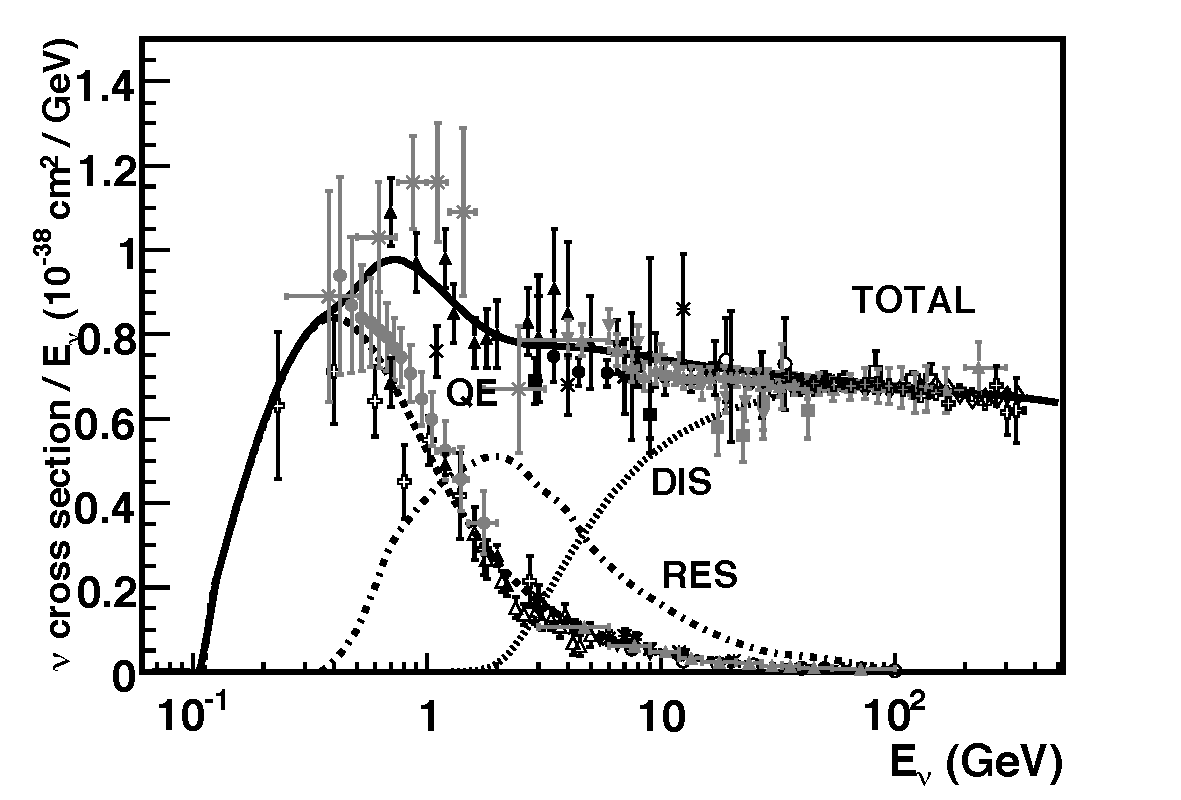
\includegraphics[width=\textwidth]{figures/theory/cc_inclusive_nu.pdf}
\caption{neutrinos}
\end{subfigure}
\begin{subfigure}[t]{0.45\linewidth}
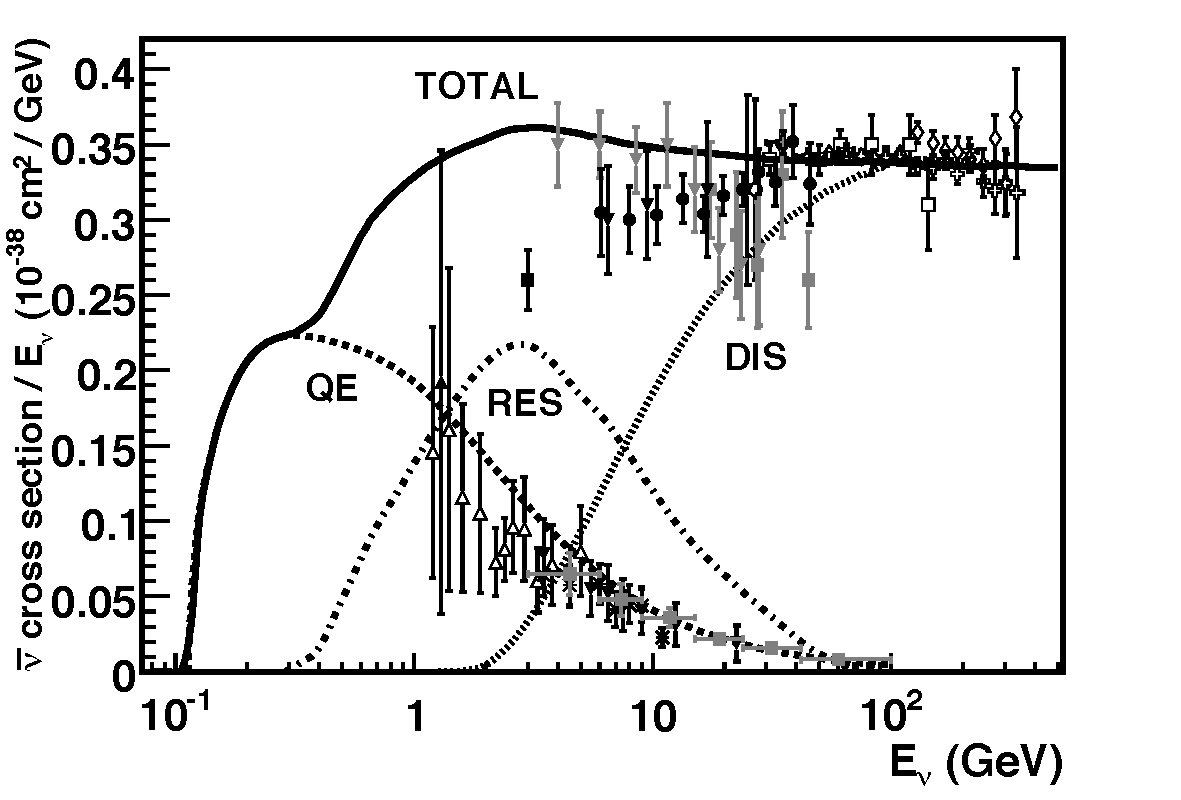
\includegraphics[width=\textwidth]{figures/theory/cc_inclusive_nubar.pdf}
\caption{antineutrinos}
\end{subfigure}
\caption{Inclusive cross sections for neutrinos and antineutrinos. Figure taken from \cite{Formaggio:2012aa}.}
\end{figure*}

\section{Neutrino Sources}
\section{Neutrino Sources}

\subsection{Solar neutrinos}
\label{sec:solar-nu}

Here we describe how solar neutrinos come to be.


\setchapterstyle{kao}
\setchapterpreamble[u]{\margintoc}
\chapter{Neutrino Masses and Oscillations}
\labch{massoscillations}

As outlined in \refsec{neutrino-masses}, flavor eigenstates of neutrinos are not identical to their mass eigenstates. After they acquire their mass via electroweak symmetry breaking, the mass and flavor eigenstates mix among each other via the PNMS matrix $U$ that, in the case of pure Dirac masses, is a $3\times3$ unitary matrix. Thus, the eigenstate for a neutrino flavor $\alpha$ can be described as a superposition of mass eigenstates as
\begin{equation}
    \ket{\nu_\alpha} = \sum_k U^*_{\alpha k}\ket{\nu_k}\;.\label{eq:flavor-state-def}
\end{equation}
This has profound consequences for the propagation of neutrinos, because the wavepackets of the different mass eigenstates do not travel at exactly the same speed. The lighter states are faster than the heavier ones, which causes the waves to interfere with one another constructively or destructively as long as the wave packets still overlap. This chapter describes neutrino oscillations in vacuum and in matter under the simplifying assumption that the mass eigenstates are ideal plane waves. The fact that they are actually wave packets with an uncertain energy and a finite extent leads to decoherence for very large propagation distances or mass differences. While this is irrelevant for the standard three-flavor oscillation result of this work, it does put an upper limit on the mass splitting for which the sterile oscillation result is valid. This will be described briefly at the end of this chapter.

\section{Neutrino Oscillations in Vacuum}

The simplest case to describe is that of neutrino oscillations in vacuum. The propagation of these states is governed by the Schrödinger equation
\begin{equation}
    i \dv{t} \ket{\nu_k(t)} = \mathcal{H} \ket{\nu_k(t)}
\end{equation}
with the plane-wave solution
\begin{equation}
    \ket{\nu_k(t)} = e^{-iE_k t} \ket{\nu_k}\;.\label{eq:schrodinger-eq}
\end{equation}
Substituting the flavor eigenstate from \refeq{flavor-state-def} into \refeq{schrodinger-eq} using the relation $U^\dag U=\mathbb{1}$, the propagation becomes
\begin{equation}
    \ket{\nu_\alpha(t)} = \sum_{\beta=e,\mu,\tau} \left(\sum_k U^*_{\alpha k} e^{-iE_k t}  U^*_{\beta k}\right) \ket{\nu_\beta}\;.\label{eq:flav-evolution}
\end{equation}
This leads directly to the expression for the probability to measure one flavor after a given time
\begin{equation}
    P_{\nu_\alpha \rightarrow \nu_\beta} = \abs{\braket{\nu_\beta}{\nu_\alpha(t)}}^2
    = \sum_{k,j}U^*_{\alpha k}U_{\beta k}U_{\alpha j}U_{\beta j}^* e^{-i(E_k - E_j)t}\;.
\end{equation}
If we assume that all mass eigenstates have the same momentum\sidenote[][*1]{The equal momentum assumption is not exactly realistic, but more detailed derivations can show that deviations from it cause no observable effect. See also chapter 8.1.2 in \cite{giunti-kim-neutrino}.} and that they are highly relativistic, we can approximately express the energy in terms of the mass of each state
\begin{equation}
    E_k = \sqrt{\vec{p}^2 + m_k^2} \simeq E + \frac{m_k^2}{2E}
\end{equation}
and write the transition probability in terms of the energy and the differences of squared masses between the mass eigenstates
\begin{equation}
    \Delta m_{kj}^2 \equiv m_k^2 - m_j^2
\end{equation}
and the travelled distance, $L$, as
\begin{equation}
    P_{\nu_\alpha \rightarrow \nu_\beta}(L,E) = \sum_{k,j}U^*_{\alpha k}U_{\beta k}U_{\alpha j}U_{\beta j}^* \exp(-i\frac{\Delta m_{kj}^2 L}{2E})\;.\label{eq:vac-oscprob}
\end{equation}
This state evolution can also be expressed with the effective Hamiltonian
\begin{equation}
    \mathcal{H}_\mathrm{eff} = \frac{1}{2E}U\mathrm{diag}(0,\Delta m_{21}^2, \Delta m_{31}^2)U^\dag
\end{equation}
and one can define the characteristic distance for oscillations between mass eigenstates $k$ and $j$ at which the oscillation amplitude is maximal as
\begin{equation}
    L_{kj}^\mathrm{osc} = \frac{4\pi E}{\Delta m_{kj}^2}\;.
\end{equation}
Antineutrino flavor eigenstates are superpositions of corresponding antineutrino mass eigenstates, and they are related by the complex-conjugated PNMS matrix such that
\begin{equation}
    \ket{\bar{\nu}_\alpha} = \sum_k U_{\alpha k}\ket{\bar{\nu}_k}\;.\label{eq:flavor-state-def-antinu}\;.
\end{equation}
This leads to the same expression for their oscillation probability as in \refeq{vac-oscprob}, except that all elements of $U$ are complex-conjugated.

\subsection{Two-neutrino mixing}
\labsubsec{two-neutrino-mixing}
Neutrino oscillation experiments are typically limited to a certain oscillation length and energy range that they can probe. Because the two mass splittings between the three known neutrino flavors are two orders of magnitude apart ($\order{\SI{e-5}{eV^2}}$ for $\Delta m^2_{21}$ vs. $\order{\SI{e-3}{eV^2}}$ for $\Delta m^2_{32}$), each experiment is in practice much more sensitive to one of them than to the other. Therefore, a good first approximation to calculate neutrino oscillation probabilities is to only consider two flavor and two mass eigenstates with a mass splitting of $\Delta m^2 \equiv m_2^2 - m_1^2$ that mix via the rotation matrix
\begin{equation}
    U =
    \begin{pmatrix}
        \cos \vartheta & \sin \vartheta \\
        -\sin \vartheta & \cos \vartheta
    \end{pmatrix}\;,\label{eq:two-flav-pnms}
\end{equation}
where the angle $\vartheta$ is the \emph{mixing angle} between the two mass eigenstates. The transition probability from flavor $\alpha$ to $\beta$ with $\alpha \neq \beta$ can be quickly derived from the general \refeq{vac-oscprob} to be
\begin{equation}
    P_{\nu_\alpha \rightarrow \nu_\beta} = \sin^2 2\vartheta \sin[2](\frac{\Delta m^2L}{4E})\qc\alpha \neq \beta\;.
\end{equation}
Conversely, the probability that an initial flavor $\alpha$ is still being measured as $\alpha$ after a given propagation distance, also referred to as the \emph{survival probability}, is
\begin{equation}
    P_{\nu_\alpha \rightarrow \nu_\alpha} = 1 - \sin^2 2\vartheta \sin[2](\frac{\Delta m^2L}{4E})\;.
\end{equation}

\section{Oscillations in matter}
The oscillation probabilities derived in the previous sections for the vacuum are altered significantly when neutrinos pass through large amounts of matter, as it is the case for neutrinos originating in the atmosphere of the Earth that pass through its dense core to be detected at the South Pole. The effect can be described as a continuous potential that is added to the Hamiltonian in the flavor basis that corresponds to the isoscalar (nulcei) targets and electrons inside the Earth. The detailed derivation of this matter potential can be found in \sidecite{matter-potentials} and we will only briefly outline the process here. We will also describe how the matter potential leads to an enhancement of effective mixing between flavors in the simplified picture of two flavors and a constant matter density.

\subsection{Effective potentials}
At energies relevant to this work\sidenote{Incoherent scattering becomes only important at energies above $\order{\SI{e5}{GeV}}$.}, neutrinos are mostly affected by coherent forward scattering processes, that is, scattering with a very small momentum transfer. The Feynman diagrams of the relevant processes are shown in \reffig{coh-scatter-feynman}. All neutrino flavors can interact with electrons and nuclei via the neutral-current (NC) interaction, while only electron-neutrinos can also undergo charged-current (CC) scattering off of electrons.
\begin{figure}
\def\flen{2}
\def\boslen{1.5}
\def\fang{25}
\begin{subfigure}[t]{0.49\linewidth}
\begin{tikzpicture}
    \begin{feynman}
        \vertex (v1) [dot] at (0, \boslen) {};
        \vertex (i1) at ($(v1) + (180-\fang:\flen)$) {$\nu_e$};
        \vertex (f1) at ($(v1) + (\fang:\flen)$) {$e^-$};

        \vertex [dot] (v2) at (0, 0) {};
        \vertex (i2) at ($(v2) + (\fang-180:\flen)$) {$e^-$};
        \vertex (f2) at ($(v2) + (-\fang:\flen)$) {$\nu_e$};

        \diagram*{
            (i1) -- [fermion] (v1) -- [fermion] (f1),
            (i2) -- [fermion] (v2) -- [fermion] (f2),
            (v1) -- [boson, edge label=$W^+$] (v2)
        };
    \end{feynman}
\end{tikzpicture}
\caption{Charged-current\label{fig:coh-scatter-cc}}
\end{subfigure}
\begin{subfigure}[t]{0.49\linewidth}
\begin{tikzpicture}
    \begin{feynman}
        \vertex (v1) [dot] at (0, \boslen) {};
        \vertex (i1) at ($(v1) + (180-\fang:\flen)$) {$\nu_e,\nu_\mu,\nu_\tau$};
        \vertex (f1) at ($(v1) + (\fang:\flen)$) {$\nu_e,\nu_\mu,\nu_\tau$};

        \vertex [dot] (v2) at (0, 0) {};
        \vertex (i2) at ($(v2) + (\fang-180:\flen)$) {$e^-, p, n$};
        \vertex (f2) at ($(v2) + (-\fang:\flen)$) {$e^-, p, n$};

        \diagram*{
            (i1) -- [fermion] (v1) -- [fermion] (f1),
            (i2) -- [fermion] (v2) -- [fermion] (f2),
            (v1) -- [boson, edge label=$Z^0$] (v2)
        };
    \end{feynman}
\end{tikzpicture}
\caption{Neutral-current}
\end{subfigure}
\caption{Feynman diagrams of the coherent forward scattering processes for neutrinos travelling through Earth.\label{fig:coh-scatter-feynman}}
\end{figure}
When the exchanged momentum is small, then the propagator in each Feynman diagram can be contracted into a 4-point Fermi interaction with the coupling constant $G_F$. The effective CC Hamiltonian for the diagram in \reffig{coh-scatter-cc} (after a Fierz transformation) becomes
\begin{equation}
    \mathcal{H}_\mathrm{eff}^{CC}(x) = \frac{G_F}{\sqrt{2}}
    [\bar{\nu}_e(x)\gamma^\rho(1 - \gamma^5)\nu_e(x)]
    [\bar{e}(x)\gamma_\rho(1 - \gamma^5)e(x)]\;.\label{eq:h-eff-cc}
\end{equation}
This Hamiltonian is then averaged over the momenta and helicities of a constant density of electrons with the result
\begin{equation}
    \overline{\mathcal{H}_\mathrm{eff}^{CC}}(x) = V_{CC} \bar{\nu}_{e,L}(x)\gamma^0\nu_{e,L}(x)\;,
\end{equation}
where $V_{CC}$ is the charged-current potential
\begin{equation}
    V_{CC} = \sqrt{2}G_F N_e
\end{equation}
with the electron number density $N_e$. The derivation of the NC potential follows in similar steps with the addition of a different coupling constant for electrons, protons, and electrons. For electrically neutral media, the potentials for protons and electrons exactly cancel and the only remaining NC potential comes from the neutron density, $N_n$, and is given by
\begin{equation}
    V_{NC} = -\frac{1}{2}\sqrt{2}G_F N_n\;.
\end{equation}
With the addition of these potentials, the effective Hamiltonian governing the evolution of flavor states for neutrinos propagating in matter is
\begin{equation}
\mathcal{H}_\mathrm{eff}(E,x) = \mathcal{H}_0(E)  + \mathcal{H}_{1}(E,x)\;,
\end{equation}
with
\begin{subequations}
\label{eq:hamiltonian}
\begin{align}
\mathcal{H}_0 (E) &= \frac{1}{2E} U
\mqty(\dmat{0 , \Delta m^2_{21}, \Delta m^2_{31}})
U^\dag \label{eq:h0-flav-basis}\;,\\
\mathcal{H}_1 (E,x) &= \frac{\sqrt{2}}{2} G_F
\mqty(\dmat{2N_e(x) - N_n(x), -N_n(x), -N_n(x)})
\;.\label{eq:hi-flav-basis}
\end{align}
\end{subequations}
The NC potential in \refeq{hi-flav-basis} can be neglected in the case of three-flavor oscillations, because a diagonal contribution to the Hamiltonian merely adds an unobservable phase shift that affects all flavors equally. However, if sterile Majorana  mass eigenstates are added, their corresponding matter potentials are zero and they only add their respective mass splitting to \refeq{h0-flav-basis}. In that case, the state evolution has to be described using both CC and NC potentials.

\subsection{The MSW Effect}
An interesting consequence of matter potentials is that they can greatly enhance the mixing amplitude between flavors over that of vacuum oscillations. The effect is straight forward to illustrate for the case of two-flavor oscillations, where one flavor feels a potential, $V$, and the other does not. With the mass-splitting $\Delta m^2 \equiv m_2^2 - m_1^2$ and $2\times2$ mixing matrix from \refeq{two-flav-pnms}, the effective Hamiltonian for this scenario is
\begin{equation}
\begin{aligned}
    \mathcal{H}  &= \frac{1}{4E}\left(
        U\mqty(\dmat{0, \Delta m^2})U^\dag + \mqty(\dmat{A_\mathrm{CC}, 0})
    \right)\\
    &= \frac{1}{4E} \mqty(
        -\Delta m^2 \cos 2\vartheta + A_\mathrm{CC} & \Delta m^2 \sin 2\vartheta \\
        \Delta m^2 \sin 2\vartheta & \Delta m^2 \cos 2\vartheta - A_\mathrm{CC}
    )\;,
\end{aligned}
\end{equation}
where we have subtracted $\frac{1}{4E}(\Delta m^2 + A_\mathrm{CC})$ from the diagonal in the second line with $A_\mathrm{CC} = 2E V$. This Hamiltonian can be diagonalized by another 2D rotation matrix $U_M$, with mixing angle $\vartheta_M$, such that
\begin{equation}
    U_M^T\mathcal{H}U_M = \mathcal{H}_M = \frac{1}{4E}\mqty(\dmat{-\Delta m^2_M, \Delta m^2_M})
\end{equation}
is diagonal. The diagonalization is achieved under the condition
\begin{equation}
    \tan 2\vartheta_M = \frac{\tan 2\vartheta}{1 - \frac{A_\mathrm{CC}}{\Delta m^2 \cos 2\vartheta}}\;,\label{eq:msw-condition}
\end{equation}
leading to a new effective mass splitting in matter,
\begin{equation}
    \Delta m^2_M = \sqrt{(\Delta m^2 \cos 2\vartheta - A_\mathrm{CC})^2 + (\Delta m^2\sin 2\vartheta)^2}\;.
\end{equation}
As a consequence of the condition in \refeq{msw-condition}, the effective mixing angle in matter can become maximal under the condition that
\begin{equation}
    V = \frac{\Delta m^2 \cos 2\vartheta}{2E_\mathrm{res}}\label{eq:msw-pot}
\end{equation}
with the resonance energy $E_\mathrm{res}$.
This enhancement of mixing between flavors due to the presence of a matter potential is known as the \emph{MSW effect}, named after Mikheev, Smirnov, and Wolfenstein. It is primarily responsible for the fact that there is a sizable disappearance of electron neutrinos from the sun despite the fact that the relevant vacuum mixing angle is rather small.
The potential for isoscalar targets is
\begin{equation}
    V = \sqrt{2}G_F N_e \approx Y_e \times \qty[\frac{\rho}{\si{\gram\per\cm\cubed}}] \times \SI{7.63e-14}{\electronvolt}\;,\label{eq:pot-isoscalar}
\end{equation}
where $Y_e = N_e / (N_p + N_n)$ is the electron fraction in the medium and is usually close to $\frac{1}{2}$.
%which corresponds to an electron number density of
%\begin{equation}
%    N_e = \frac{\Delta m^2 \cos 2\vartheta}{2\sqrt{2}E G_F}\;.\label{eq:msw-electron-density}
%\end{equation}
%Taking the density of the core of the Earth, $\rho_\mathrm{core} \approx \SI{13}{\gram\per\cubic\centi\meter}$, we find
%\begin{equation}
%    N_{e,\mathrm{core}} \approx \SI{13}{\gram\per\cubic\centi\meter}\times \frac{1}{2} \times \SI{1}{\mole\per\gram} \times N_A \approx \SI{4e24}{\per\cubic\centi\meter}\;,
%\end{equation}
%we find
We can find the resonant energy where the MSW resonance occurs for a given matter density by combining \cref{eq:msw-pot,eq:pot-isoscalar} into
\begin{equation}
    E_\mathrm{res} = \frac{\Delta m^2 \cos 2\vartheta}{2V} \approx \frac{(\Delta m^2\si{\per\electronvolt\squared}) \cos 2\vartheta}{Y_e \qty[\frac{\rho}{\si{\gram\per\cm\cubed}}]}\times\SI{6.6e12}{\electronvolt}\;.
\end{equation}
For three-flavor oscillations observed experimentally, the MSW resonance can enhance mixing due to the relatively small mixing angle $\theta_{13}=\SI{8.6+-0.13}{\degree}$\cite{pdg}.  This occurs at $\approx \SI{7}{\giga\electronvolt}$ for muon neutrinos travelling through the mantle of the Earth, where the density is $\rho_\mathrm{mantle}\approx\SI{4.5}{\gram\per\cubic\centi\meter}$ and where the observed oscillations are due to the larger mass splitting $\Delta m^2_{32}\approx \SI{2.5e-3}{\electronvolt\squared}$.
For hypothetical sterile neutrinos with a mass splitting of $\order{\SI{1}{\electronvolt}}$ passing through the core of the Earth with $\rho\approx\SI{13}{\gram\per\cubic\centi\meter}$ and $Y_e\approx\frac{1}{2}$, this gives a resonant energy of close to \SI{1}{\tera\electronvolt} assuming a small mixing angle between active and sterile flavors. This effect has been used in previous IceCube studies\cite{MEOWS} to search for traces of sterile neutrinos using TeV~scale atmospheric neutrinos, but it is not relevant to the analysis presented in this work.

\subsection{Parametric resonance}
Another way in which the presence of matter potentials can enhance neutrino oscillation amplitudes is via parametric resonance. This resonance occurs when the matter potential changes abruptly at just the right frequency to create a situation that is analogous to constructive interference, even if the density is far from the MSW resonance condition. The reason why this can happen is that the quantum state of the neutrino receives a phase shift at every interface between regions of different densities. If such an interface is located at the oscillation maximum and the difference in densities has the right magnitude, the phase is reset to zero and and the flavor transition probability will increase again in the next region, instead of returning to zero. This situation can arise in particular at the transition points between the mantle and the core when neutrinos pass through the Earth as shown in \reffig{parametric-resonance}. The black solid line shows the matter potential that is used to approximate the matter potential for the oscillation calculation. At each interface (dashed lines), the phase shift causes the oscillation pattern to begin at the rising flank again. After the neutrino propagates through the Earth, the oscillation probability has increased to close to one.
\begin{figure}
    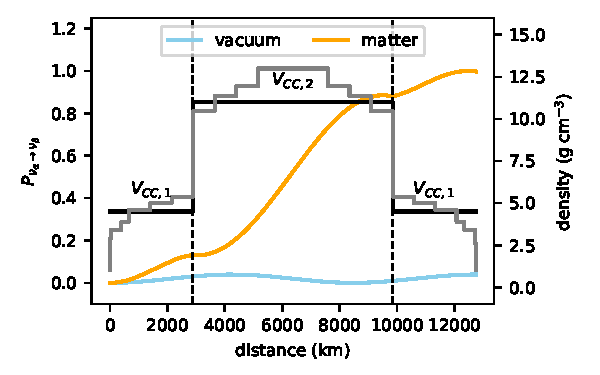
\includegraphics[width=4in]{figures/theory/parametric_resonance.pdf}
    \caption{Parametric resonance for a simplified mantle-core-mantle propagation with two flavors. The assumed mass-splitting is $\Delta m^2=\SI{2.5e-3}{eV^2}$, the mixing angle is $\theta=\arcsin(0.1)$, and the energy is \SI{3.4}{GeV}. The matter potential used for the calculation is shown in black. The gray line in the background shows the density profile of Earth in the 12-layer PREM model.\label{fig:parametric-resonance}}
\end{figure}
The condition for maximum parametric resonance is delicately dependent on the energy, mass splitting, mixing angle, and the parameters of the matter potential and are derived in more detail in \cite{Akhmedov:1999ty}. In atmospheric neutrino oscillations, parametric enhancement of the $\nu_\mu\rightarrow\nu_e$ oscillation channel is responsible for the distortions of the oscillation pattern at a few GeV.


\subsection{Neutrino Mass Ordering}
In vacuum, neutrino oscillations are only sensitive to the absolute differences between (squared) neutrino masses, not their sign. As a result, there are two degenerate possibilities to arrange the mass eigenstates that produce the same vacuum oscillation effect. The case where $m^2_1 < m^2_2 < m^2_3$ is referred to as \emph{normal ordering}. In this case, the value of the mass splitting $\Delta m^2_{ij}$ is always positive for $i>j$. In the case of \emph{inverted ordering}, we have $m^2_3 < m^2_1 < m^2_2$. In that case, the sign of $\Delta m^2_{32}$ is negative. While the ordering has no observable effect in vacuum, it does affect the propagation in the presence of matter effects. This can be seen readily in the MSW resonance condition in \refeq{msw-condition}, where the sign of $\Delta m^2$ enters in the denominator. The resonance condition for neutrinos can only be fulfilled if the sign of $\Delta m^2$ is the same as $\cos 2\theta$ for neutrinos, or if the signs of $\Delta m^2$ and $\cos 2\theta$ are different for antineutrinos. Therefore, the neutrino mass ordering can be determined experimentally by measuring the differences in matter effects between neutrinos and antineutrinos.

\section{Standard three-flavor oscillations}
The simplest extension to the Standard Model that explains the phenomenon of neutrino oscillations is that of three oscillating flavor eigenstates and three mass eigenstates that result from pure Dirac masses as described in \refsec{neutrino-masses}. In this picture, the mixing between mass eigenstates and is governed by the $3\times3$ PNMS matrix that is commonly parametrized by three mixing angles and one complex phase
\begin{equation}
\begin{aligned}
    U &=
    \begin{pmatrix}
    U_{e1}    & U_{e2}    & U_{e3}    \\
    U_{\mu1}  & U_{\mu2}  & U_{\mu3}  \\
    U_{\tau1} & U_{\tau2} & U_{\tau3} \\
    \end{pmatrix} \\
    &=
    \begin{pmatrix}
        c_{12} c_{13} & s_{12} c_{13} & s_{13}e^{-i\delta}       \\
        -s_{12}c_{23} - c_{12}s_{23}s_{13}e^{i\delta} & c_{12}c_{23}-s_{12}s_{23}s_{13}e^{i\delta} & s_{23}c_{13} \\
        s_{12}s_{23}-c_{12}c_{23}s_{13}e^{i\delta} & -c_{12}s_{23}-s_{12}c_{23}s_{13}e^{i\delta} & c_{23}c_{13}
    \end{pmatrix}\;,
\end{aligned}\label{eq:pnms-parametrization}
\end{equation}
where $s_{ij}$ and $c_{ij}$ are, respectively, the sine and cosine of the mixing angle $\theta_{ij}$. The complex phase $\delta$ leads to CP-violation of the oscillations. In addition, there are two mass splitting values between the three mass eigenstates, $\Delta m^2_{21}$ and $\Delta m^2_{31}$, that govern the frequency of the oscillations.
The most recent global best fit point\cite{Esteban:2020cvm} of the mixing angles and mass splittings under the assumption of normal neutrino mass ordering is shown in \reftab{global-bfp}. The table also lists the experimental channels that are primarily used to measure each parameter\todo{make table a bit nice, maybe include IO}.
\begin{table}
\caption{Best fit values of three-flavor oscillation parameters and the oscillation channel that is primarily involved in their measurement.\label{tab:global-bfp}}
\begin{tabular}{ccc}\toprule
    parameter & global fit & experimental channel \\ \midrule
    $\theta_{12}/^\circ$                    & $33.44^{+0.77}_{-0.74}$   & $\nu_e \rightarrow \nu_e$ (solar)\\
    $\frac{\Delta m^2_{21}}{\SI{e-5}{eV^2}}$& $7.42^{+0.21}_{-0.20}$    & $\bar{\nu}_e \rightarrow \bar{\nu}_e$ (reactor)\\
    $\theta_{23}/^\circ$                    & $49.2^{+1.0}_{-1.3} $     & $\nu_\mu \rightarrow \nu_\mu$  (atmospheric, accelerator)\\
    $\frac{\Delta m^2_{31}}{\SI{e-3}{eV^2}}$& $2.515^{+0.028}_{-0.028}$ & \\
    $\theta_{13}/^\circ$                    & $8.57^{+0.13}_{-0.12} $   & $\bar{\nu}_e \rightarrow \bar{\nu}_e$ (reactor)\\
    $\delta_\mathrm{CP}/^\circ$             & $194^{+52}_{-25}$         & $\nu_\mu \rightarrow \nu_e$ (accelerator)\\ \bottomrule
\end{tabular}
\end{table}
This section outlines the current global picture of neutrino oscillation measurements and briefly describes the types of experiment that probe the oscillation parameters.

\subsection{Types of oscillation experiments}

Different neutrino oscillation experiments probe different parts of the PNMS matrix and mass splitting. Broadly speaking, experiments can be divided into two categories by the mass-splitting that they can probe, which is determined by the oscillation length and energy spectrum of the experimental setup. The requirement to resolve oscillations is that the argument of the oscillation is $\Delta m^2 L/(2E) \sim \order{1}$. The larger of the two mass splittings is $\Delta m^2_{21} \sim \order{\SI{e-5}{eV^2}}$ and the smaller mass splitting is $\abs{\Delta m^2_{31}} \sim \order{\SI{e-3}{eV^2}}$. \reffig{oscillation-experiments-overview} gives an overview over different experiments, both operational and planned, with their respective energy ranges and baselines.
\begin{figure}
    \centering
    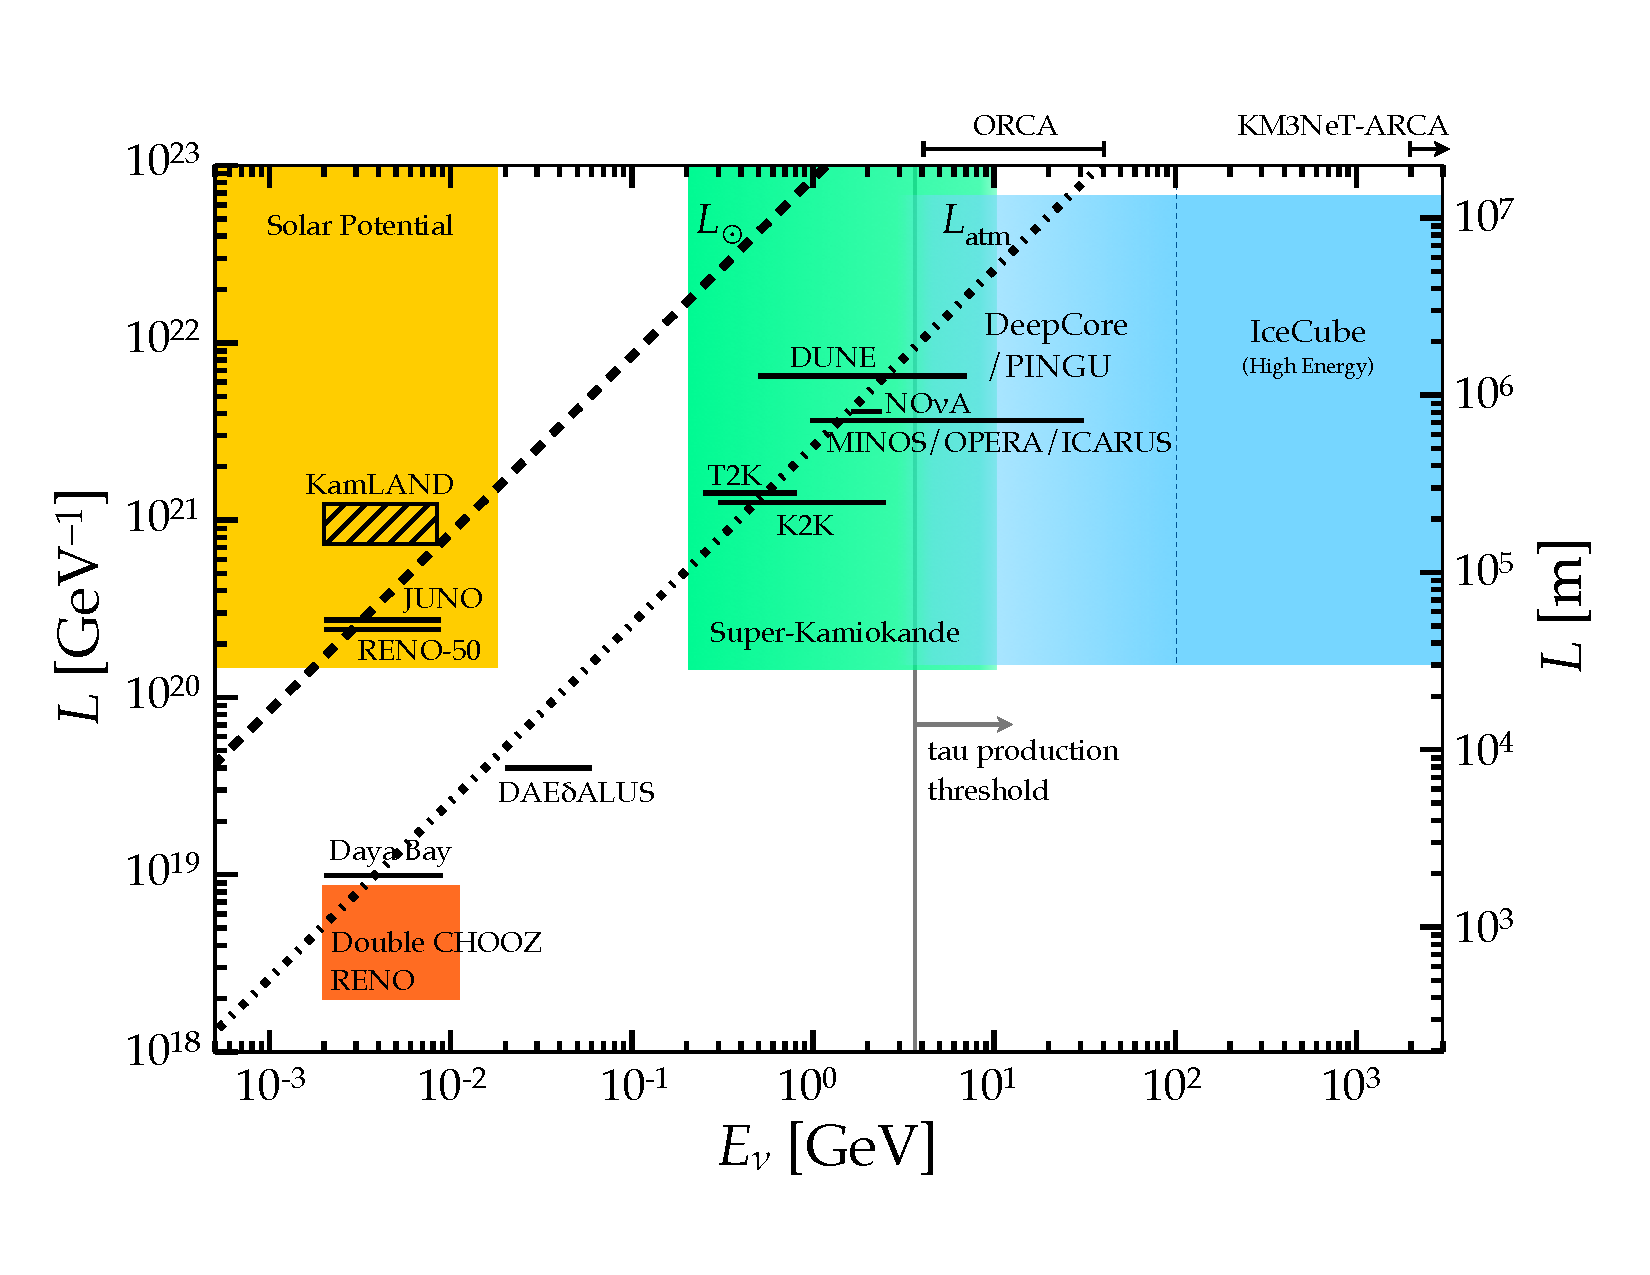
\includegraphics{figures/theory/LvsE.pdf}
    \caption{Energy ranges and baselines for a selection of neutrino oscillation experiments, operational or planned. Experiments on the line marked $L_{\odot}$ probe the solar mass splitting of $\order{\SI{e-5}{eV^2}}$, while those on the line marked $L_\mathrm{atm}$ measure oscillations at the atmospheric mass splitting of $\order{\SI{e-3}{eV^2}}$. The range of each experiment is shown either as a line for experiments with a fixed oscillation distance such as T2K or DUNE, or as a box for experiments with both a variable baseline and energy range such as IceCube. Figure taken from\cite{IceCube:2016xxt}.\label{fig:oscillation-experiments-overview}}
\end{figure}

\subsubsection{Solar neutrinos}
The mixing angles that parametrize the PNMS matrix and the mass splittings are typically associated with types of experiments that are most sensitive to them based on the oscillation channel that they observe. Since the angle $\theta_{13}$ is small, the PNMS matrix in \refeq{pnms-parametrization} can be decomposed to a first approximation into the upper left and lower right $2\times2$ blocks. The upper left block governs the transitions between $\nu_e$ and $\nu_\mu$ flavors with the mixing angle $\theta_{12}$ and the small mass splitting $\Delta m^2_{21}$. Such transitions are observed mainly by measurements of the neutrino flux originating from the Sun. For this reason, the mixing angle $\theta_{12}$ is also referred to as the ``solar angle`` and $\Delta m^2_{21}$ as the ``solar mass splitting``. Measurements of the solar neutrino flux are the oldest hints at neutrino oscillations and began at the end of the 1960s with the Homestake\cite{DAVIS199413} experiment. It used the inverse beta-decay process $^{37}\mathrm{Cl}+\nu_e \rightarrow e^- + ^{37}\mathrm{Ar}$ to capture neutrinos with an energy threshold of \SI{0.814}{MeV}. The observed neutrino flux was only about 30\% of the expectation, giving rise to the \emph{solar neutrino problem}. More recently, the Sudbury Neutrino Observatory (SNO) confirmed\cite{PhysRevC.88.025501} that this deficit is due to a conversion of electron neutrinos into muon neutrinos, while the total neutrino flux, as measured by the rate of neutral-current interactions, stays constant. Terrestrially, these oscillations can only be observed using very low energy neutrinos from nuclear fission reactors at baselines of hundreds of kilometers. The only experiment of this kind that is currently operational is the KamLAND detector\cite{PhysRevLett.90.021802}.

\subsubsection{Atmospheric and accelerator neutrinos}
The lower right block of the PNMS matrix controls transitions between $\nu_\mu$ and $\nu_\tau$ flavors with the mixing angle $\theta_{23}$ and large mass splitting $\Delta m^2_{32}$. These transitions are primarily observed by measuring the survival probability of muon neutrinos that are produced in the atmosphere of the Earth. Therefore, $\Delta m^2_{32}$ and $\theta_{23}$ are referred to as the ``atmospheric`` mass splitting and mixing angle, respectively. The first experiment that was able to measure the effect of atmospheric neutrino oscillations is the Super-Kamiokande experiment\cite{PhysRevLett.81.1562}, a Cherenkov neutrino detector located in the Kamioka mountains in Japan. The details of atmospheric neutrino oscillation measurements are of special interest to this work and are described in more detail in \refsec{atmospheric-neutrino-oscillations}. The same oscillation channel is also accessible via long-baseline accelerator neutrino experiments. These experiments use neutrinos that are produced when protons are shot at a stationary target by a particle accelerator. The interactions of the protons with the target produce a hadronic shower consisting mostly of pions that are then focused into a tube where they are allowed to decay into neutrinos and charged leptons. This process is very similar to the production of neutrinos in the atmosphere and leads to a beam that is composed of mostly muon neutrinos and some electron neutrinos. The beam is targeted at a detector that is typically located several hundreds of kilometers away from the neutrino production site. An example for such an experimental setup is the MINOS experiment\cite{MICHAEL2008190}. \reffig{numi-beam} shows the setup of the Neutrino Main Injector (NuMI) that produces neutrinos for MINOS at a peak energy of \SI{3}{GeV}. The neutrino flux is measured at a near and a far detector at baselines of \SI{1}{km} and \SI{735}{km}, respectively, that are both identically constructed magnetized steel-scintillator tracking calorimeters. The atmospheric mass splitting and mixing angle can be estimated by comparing the neutrino flux at the near and far detectors, such that most of the inherent systematic uncertainties of the measurement cancel out. Other experiments with a similar setup are T2K\cite{T2K:2011qtm} and NO$\nu$A\cite{Patterson:2012zs}.
\begin{figure*}
    \centering
    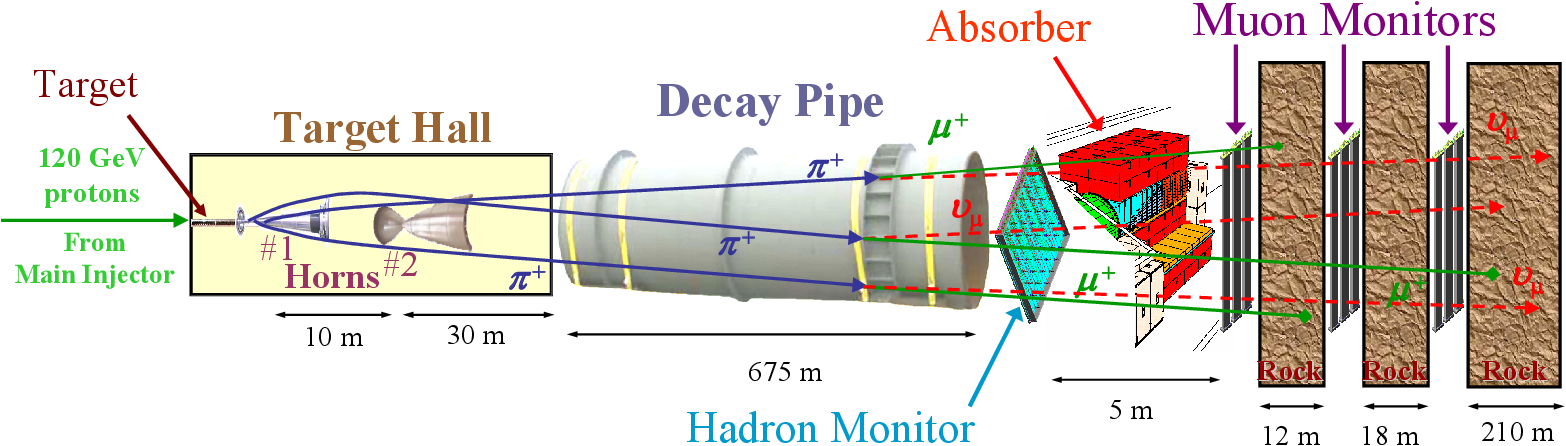
\includegraphics{figures/theory/numi_beam.png}
    \caption{Neutrino Main Injector (NuMI) facility producing neutrinos for the MINOS experiment. Figure taken from\cite{osti_879065}.\label{fig:numi-beam}}
\end{figure*}

\subsubsection{Reactor neutrinos}
The effect of the smaller mixing angle $\theta_{13}$ is in the sector of electron is that of a disappearance of electron neutrinos at short distances. Such measurements can be made using electron antineutrinos that are produced by fission reactors. Thus, the angle $\theta_{13}$ is also called the ``reactor`` angle. One experiment that is undertaking such measurements is the Daya Bay Reactor Neutrino Experiment\cite{DayaBay:2007fgu}. It consists of several detectors arranged around the reactor cores of the Daya Bay nuclear power plant that measure the electron antineutrino flux at different baselines. Comparative measurements between these detectors allows the mixing angle $\theta_{13}$ to be precisely determined while cancelling most of the systematic uncertainties of the experiment.


\section{Atmospheric Neutrino Oscillations}
\labsec{atmospheric-neutrino-oscillations}
This work presents two analyses based on the measurement of oscillations of neutrinos that are produced in the atmosphere of the Earth. This section describes how neutrinos are produced in the atmosphere and which oscillation phenomena occur when they travel through the Earth before being detected by the IceCube observatory at the South Pole.

\subsection{Neutrino production in the atmosphere}
Neutrinos are produced in the atmosphere of the Earth when highly energetic cosmic radiation interacts with its upper layers. This cosmic radiation is composed of mostly fast protons and helium nuclei, and to a smaller fraction of other elements. The composition and spectrum of this radiation has been measured extensively by experiments conducted at high altitudes, such as in weather balloons, satellites, and on the International Space Station. The flux of cosmic rays as a function of energy per particle is shown in \reffig{cr-primary-flux}. From a few GeV to approximately \SI{100}{TeV}, it can be well approximated by a power spectrum with a spectral index of $\gamma \approx 2.7$.
\begin{figure}
    \centering
    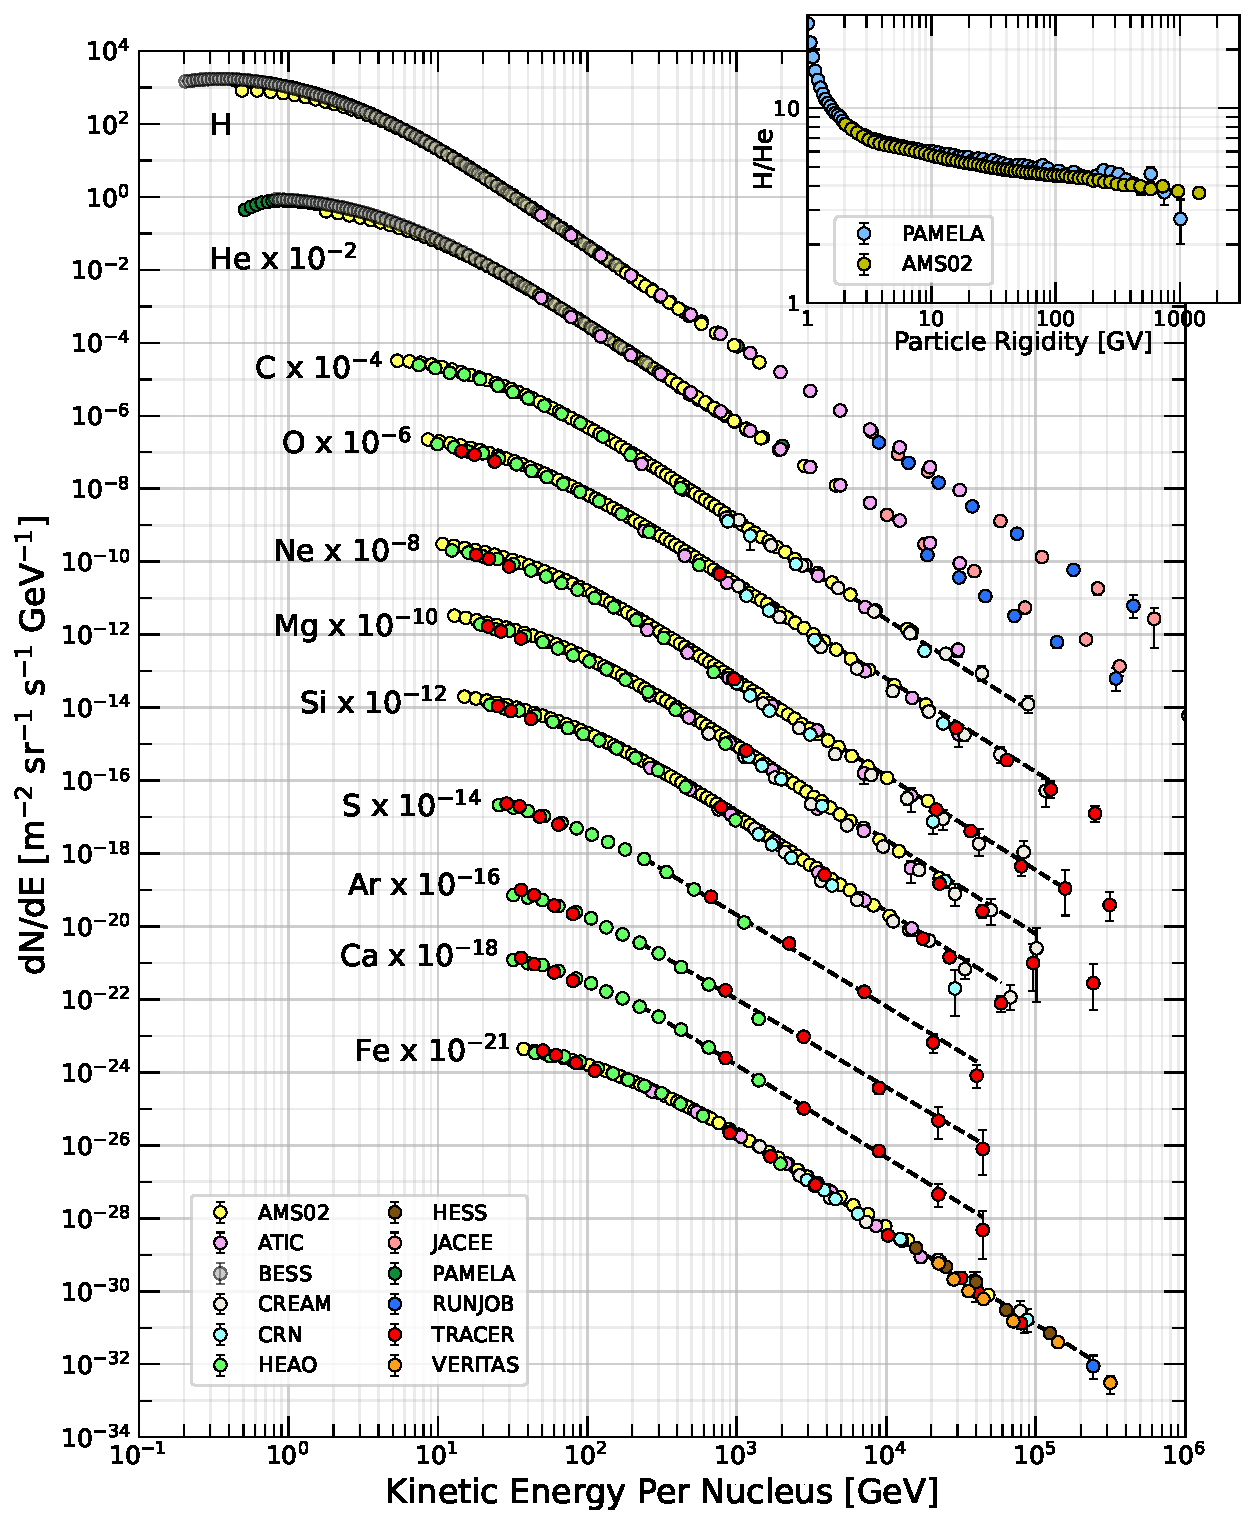
\includegraphics{figures/flux/2021_Figure_1_Inset_v1.pdf}
    \caption{Spectrum of primary cosmic rays and its components as a function of the kinetic energy. The inset shows the hydrogen to helium fraction as a function of rigidity, which is defined as the gyroradius of the ray multiplied by the magnetic field strength $R=r_L B$. Figure taken from \cite{pdg}.\label{fig:cr-primary-flux}}
\end{figure}
When a cosmic ray interacts with a nucleus, it creates a shower of hadrons that is mostly composed of Pions and Kaons that subsequently decay into muons, electrons, and neutrinos in the reaction chain
\begin{equation}
    \begin{aligned}
        \mathrm{C.R.} + N & \rightarrow X + \pi^\pm, K^\pm \\
        \pi^\pm & \rightarrow \mu^\pm + \pbar{\nu}_\mu \\
        \mu^\pm & \rightarrow e^\pm + \pbar{\nu}_e + \pbar{\nu}_\mu\;.
    \end{aligned}
\end{equation}
At energies of $\order{\SI{1}{GeV}}$, these reactions lead to a production of muon neutrinos and electron neutrinos at a ratio of $2:1$. As the energy increases, however, muons can increasingly reach the surface of the Earth and interact before they can decay, which increases the relative fraction of muon neutrinos as shown in \reffig{flux-numu-ratio}. Between GeV and TeV energies, the $\nu_\mu$ flux has a spectral index that is similar to that of the primary cosmic rays at $\gamma \approx 2.7$ as can be seen in \reffig{flux-alldir}, while the spectrum for electron neutrinos falls off more quickly at higher energies. Tau neutrinos can also be produced if a cosmic ray interaction produces charmed mesons, but such interactions are rare and the atmospheric tau neutrino flux is below 0.1\% for the energies considered in this work\cite{fedynitch2015calculation} and is therefore neglected.
\begin{figure}
\centering
\begin{subfigure}[t]{0.55\linewidth}
    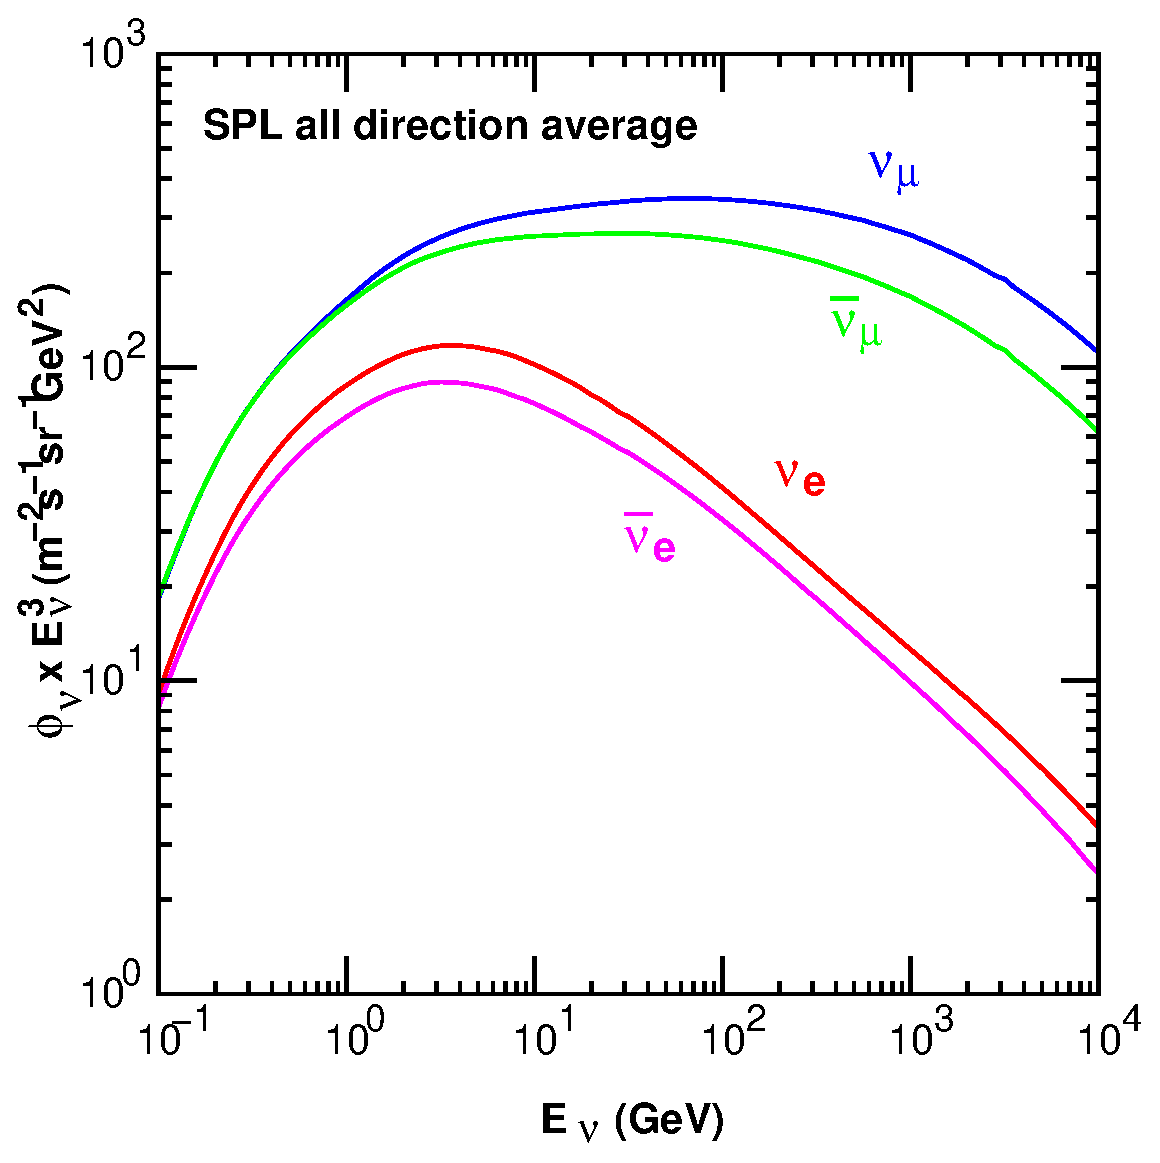
\includegraphics[height=2.2in]{figures/flux/alldir-spl.eps}
\caption{Neutrino flux averaged over all directions\label{fig:flux-alldir}}
\end{subfigure}
\hfill
\begin{subfigure}[t]{0.35\linewidth}
    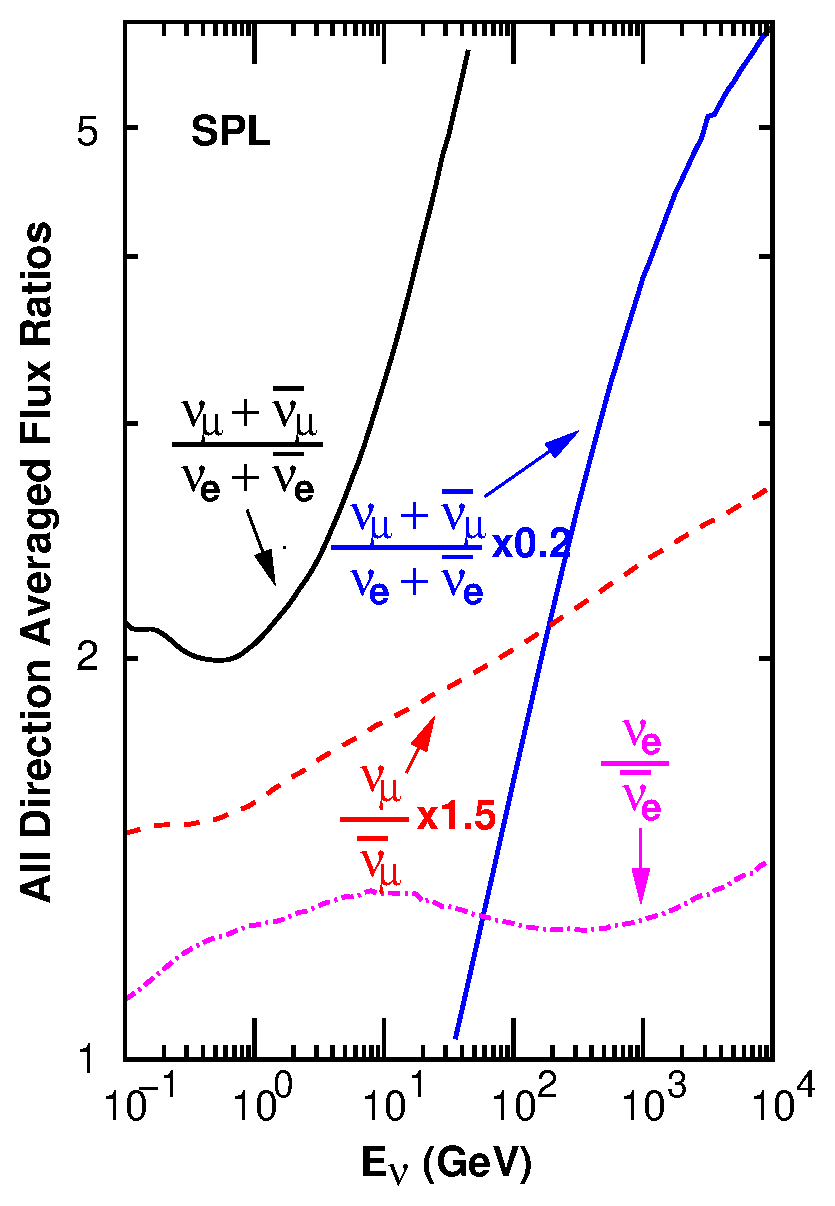
\includegraphics[height=2.2in]{figures/flux/spl-ratio-ally.eps}
\caption{Ratio of muon neutrinos to electron neutrinos\label{fig:flux-numu-ratio}}
\end{subfigure}
\caption{Neurino flux at the South Pole, averaged over all directions. Figures taken from \cite{Honda:2015fha}.}
\end{figure}

\subsection{Three-flavor oscillations of atmospheric neutrinos}
After neutrinos are produced in the atmosphere, they travel through the Earth before they are detected at the South Pole. Depending on the zenith angle at which a neutrino is observed, it has travelled a total distance, $L$, that depends on the radius of the Earth, $R_\oplus$, the depth of the detector, $d_\mathrm{det}$, and the production height of the neutrino, $h_\mathrm{atm}$, as illustrated in \reffig{atmo-baseline-illustration}. From the geometry, $L$ is calculated as
\begin{equation}
    L = (d - R_\oplus)\cos(\theta_z) + \sqrt{(R_\oplus + h_\mathrm{atm})^2 - (R_\oplus - d)^2\sin^2(\theta_z)}\;.\label{eq:prop-distance}
\end{equation}
\begin{figure}
    \centering
    \tikzsetnextfilename{atmo_baseline_illustration}%
\begin{tikzpicture}
    \def\Rearth{2.6}
    \def\Rcore{1.3}
    \def\Ratmo{3}
    \def\detpos{-2.2}
    \draw[name path=atmo, fill=cyan!50!white] (0,0) circle (\Ratmo);
    \shadedraw[
        outer color=brown!70!black,
        inner color=brown!40!white,
        name path=earh,
        %postaction={decorate},
        %decoration={raise=2pt, text along path, text={Earth}, text align=center}
    ] (0,0) circle (\Rearth);
    \shade[outer color=brown!70!black,inner color=brown!40!white, name path=earh] (0,0) circle (\Rcore);
    \node [draw, thick, shape=rectangle, minimum width=0.3cm, minimum height=0.4cm, anchor=center, fill=gray] (detector) at (0, \detpos) {};
    \path [name path=nupath] (detector) +(55:6) -- +(235:1);
    \draw [name intersections={of=nupath and atmo, by={a,b}}, -stealth, very thick] (a) -- node[above, sloped] {$L$} (b);
    \draw [name intersections={of=nupath and atmo, by={a,b}}, thick] (detector.center) --  node [sloped, above, pos=0.6] {$R_\oplus - d_\mathrm{det}$} (0,0) -- node [sloped, above] {$R_\oplus + h_\mathrm{atm}$} (a);
    \draw (detector) +(90:0.4) arc (90:235:0.4) node[midway, anchor=east] {$\theta_z$};
    \draw [stealth-stealth] (0,0) -- node [above] {$R_\oplus$} (150:\Rearth);
    \draw [stealth-stealth] (150:\Rearth) -- node [draw,above=0.2cm, fill=white] {$h_\mathrm{atm}$} (150:\Ratmo);
    \draw (detector.center) -- (detector -| 0.5,0);
    \draw (0, -\Rearth) -- (0.5, -\Rearth);
    \draw [stealth-stealth] (0.5, -\Rearth) -- node[draw, fill=white, right=.1cm] {$d_\mathrm{det}$} (detector -| 0.5,0);
    \node [anchor=north] at (0,\Rearth) {\footnotesize mantle};
    \node [anchor=north] at (0,\Rcore) {\footnotesize core};
\end{tikzpicture}

    \caption{Illustration of the geometry of atmospheric oscillation measurements. The detector is shown as the gray box near the bottom and $\theta_z$ indicates the observed zenith angle of a neutrino.\label{fig:atmo-baseline-illustration}}
\end{figure}
If the height of the atmosphere and detector depth is neglected, \refeq{prop-distance} reduces to
\begin{equation}
    L =
    \begin{cases}
        0 & \theta_z \leq \frac{\pi}{2} \\
        2 R_\oplus \cos \theta_z & \theta_z > \frac{\pi}{2}
    \end{cases}\;.
\end{equation}
From the perspective of the IceCube detector, an \emph{up-going event} is one where the zenith angle is $\theta_z > \ang{90}$, that is, $\cos(\theta_z) < 0$. On the other hand, a \emph{down-going} event is one where $\cos(\theta_z) > 0$. In such cases, the neutrino travels only through the atmosphere and the overburden of the detector and therefore matter effects are negligible.  The Earth is modeled as a set of concentric shells with different matter densities. The most prominent feature in the density profile is the core region at a depth of close to half an Earth radius, where the density sharply increases from \SI{5}{\gram\per\centi\meter\cubed} to \SI{>10}{\gram\per\centi\meter\cubed}\cite{PREM}. Neutrinos for which $\cos(\theta_z) \lesssim 0.8$ travel partially through the core and generally experience greatly enhanced matter effects. Given the baseline of $\order{R_\oplus\sim\SI{e4}{km}}$ and the core energy range of the atmospheric neutrino spectrum between GeV and TeV scales, the mass splitting between mass eigenstates whose oscillation could be observed $\SI{e-4}{eV^2} < \Delta m^2 < \SI{e-1}{eV^2}$.

Since the primary constituent of the atmospheric neutrino flux are muon (anti-)neutrinos, the most important oscillation channel to be observed is the muon neutrino survival probability.

\section{Anomalies in neutrino oscillation measurements}
While the three-flavor oscillation picture explains most of the experimental data from reactor, accelerator, atmospheric and solar neutrino experiments fairly well, there are some notable exceptions of anomalous experimental observations. These anomalies are
\begin{itemize}
    \item Reactor Antineutrino Anomaly: A deficit of $\bar{\nu}_e$ in the neutrino flux of nuclear reactors with respect to the theoretical flux expectation at baselines between $L\sim\SI{10}{m}$ and $L\sim\SI{100}{m}$.
    \item LSND anomaly: An excess of $\bar{\nu}_e$ in the neutrino flux of a proton-on-target (accelerator) source at $L\sim\SI{30}{m}$ and $E\sim\SI{30}{MeV}$.
    \item MiniBooNE anomaly: Excess of electron-like events in the the flux of neutrinos generated by an accelerator source at $L\sim\SI{500}{m}$ and $E\sim\SI{500}{MeV}$.
    \item Gallium anomaly: A deficit of $\nu_e$ in the flux of a radioactive $^{51}\mathrm{Cr}$ source. The detector is in direct contact with the source and is of $\order{\SI{1}{m}}$ in size in each dimension.
\end{itemize}
This section summarizes each of these measurements and describes how they could be resolved by the introduction of sterile neutrino states.

\subsection{Reactor neutrino anomaly}
The Reactor Antineutrino Anomaly (RAA) was first described in 2011\sidecite{Mention:2011rk} after new corrections were introduced into the theoretical calculations to the predicted neutrino flux from commercial nuclear reactors. The corrections adjusted the predicted flux upwards, leaving a deficit of $\sim 6\%$ in the measured flux with respect to the new prediction. It is suggested in \cite{Mention:2011rk} that this deficit could be explained by the introduction of an additional mass eigenstate with a mass splitting, $\Delta m^2_{41}$, and mixing angle, $\theta_{14}$. The electron neutrino survival probability can be approximated for distances of $L\lesssim \SI{1}{km}$ as
\begin{equation}
    P_{ee} = 1 - \cos^4 (\theta_{14}) \sin^2 (2\theta_{13}) \sin^2 \left(\frac{\Delta m^2_{31} L}{4E} \right) - \sin^2 (2\theta_{14}) \sin^2 \left(\frac{\Delta m^2_{14} L}{4E} \right)\;.
\end{equation}
The magnitude of the additional mass splitting and mixing angle proposed in \sidecite{Mention:2011rk} is $\abs{\Delta m^2_{41}} \gg \SI{1}{eV^2}$ and $\sin^2(2\theta_\mathrm{new})=0.12$, respectively. The oscillations due to this mass eigenstate would be too fast to be resolvable and would only lead to an average deficit that is shown as the blue line in \reffig{raa}. The red line shows the flux expectation in the presence of only three active flavors.
\begin{figure}
    \centering
    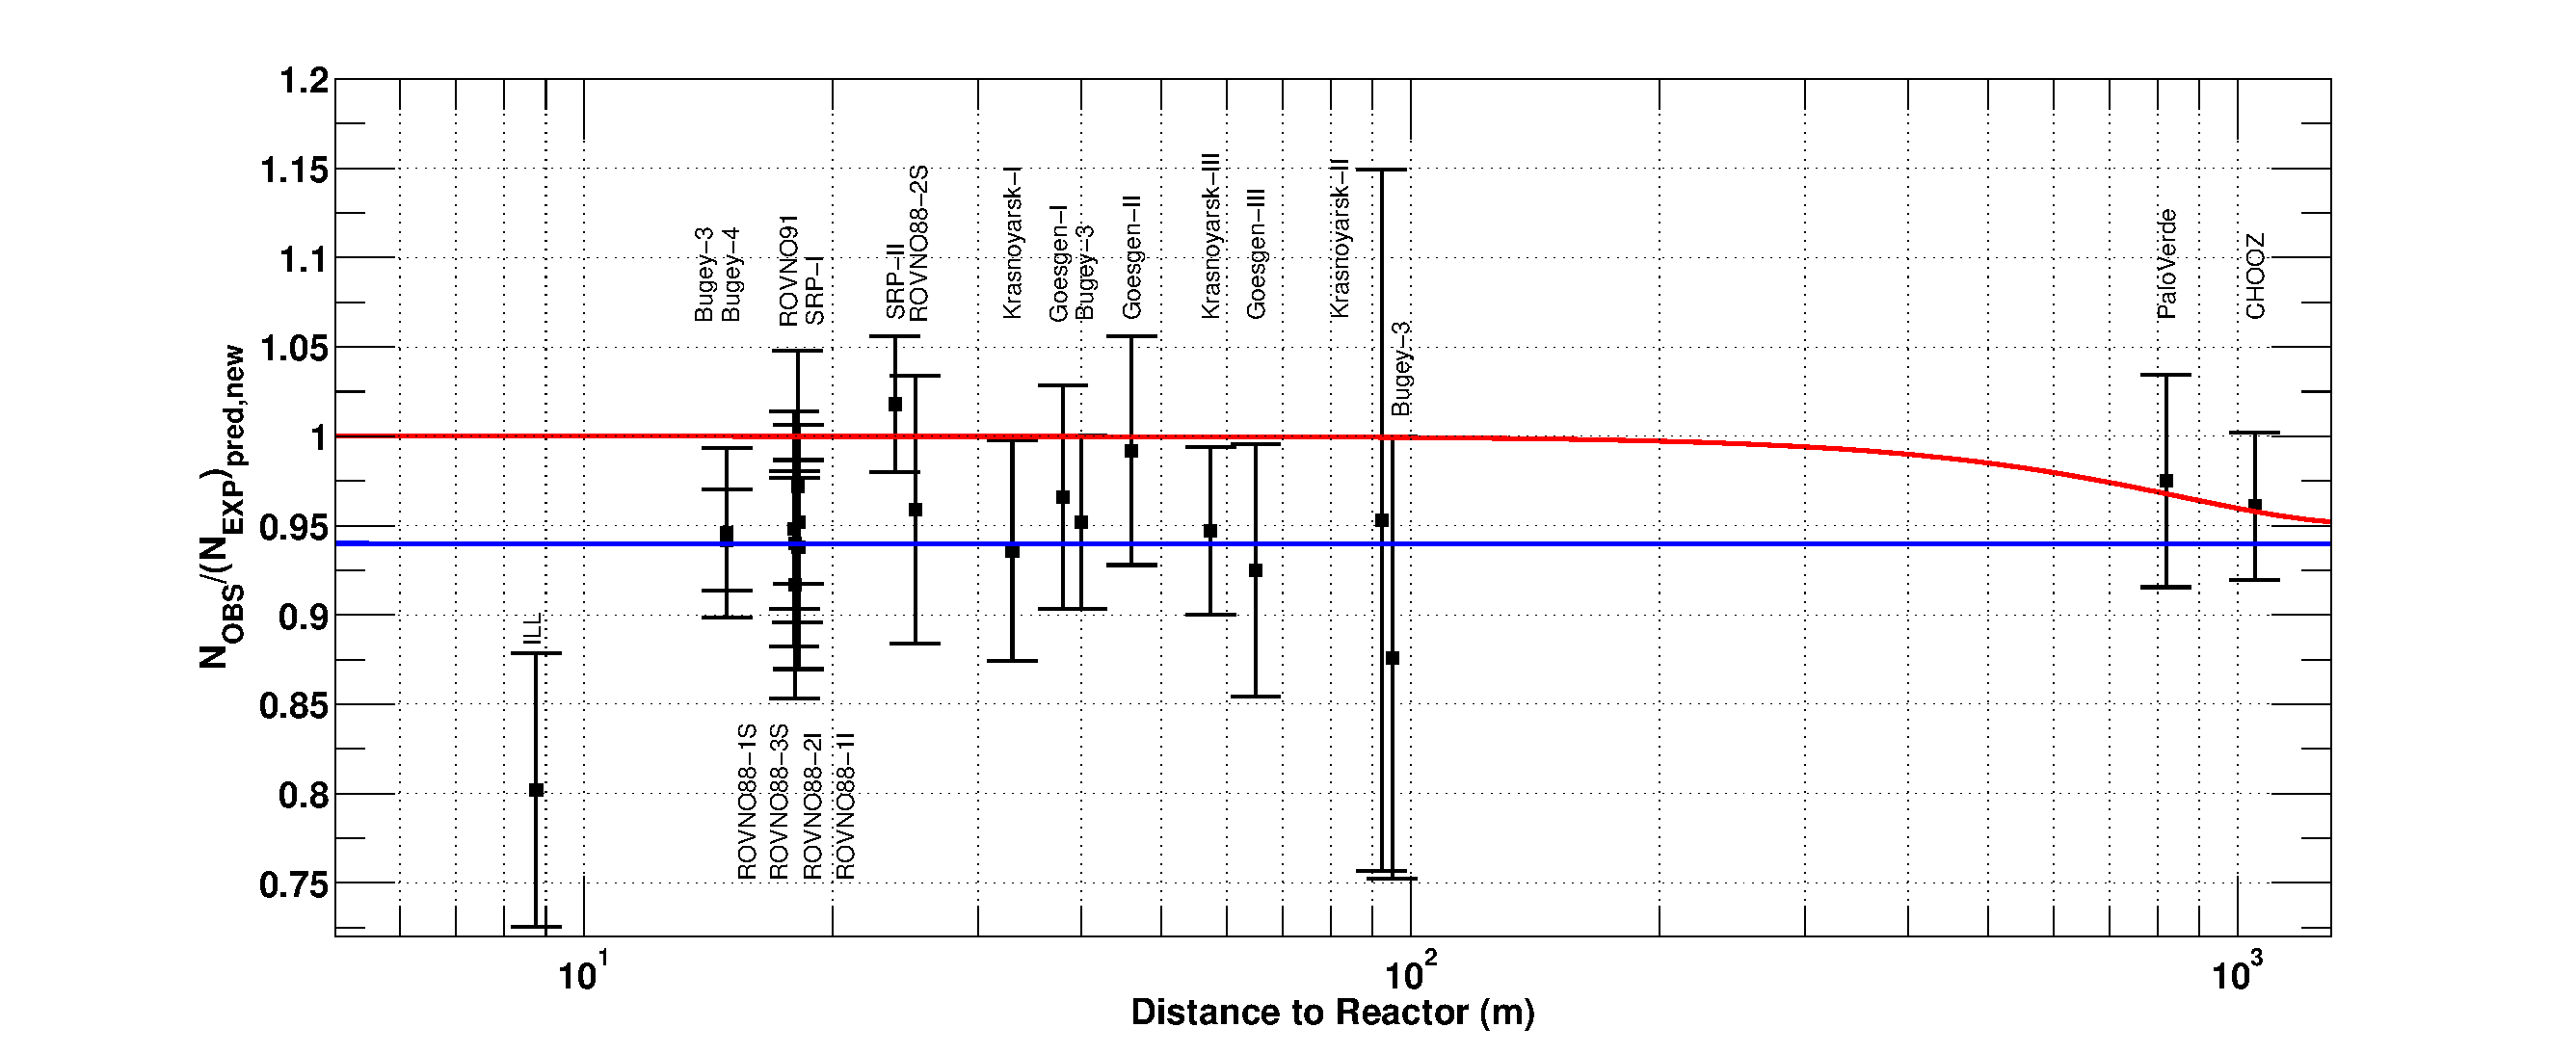
\includegraphics{figures/theory/raa.pdf}
    \caption{Deficit in $\bar{\nu}_e$ flux from commercial nuclear reactors referred to as Reactor Antineutrino Anomaly. Figure taken from \cite{Mention:2011rk}.\label{fig:raa}}
\end{figure}
Whether or not the RAA truly is an anomaly depends on whether or not one trusts the theoretical flux predictions. The involved calculations require complex nuclear corrections to the Weak interactions that are not perfectly understood. The RAA is, in fact, not the only anomaly in the reactor antineutrino flux. The second anomaly, an excess of $\bar{\nu}_e$ at $\sim \SI{5}{MeV}$, is thought to originate from poorly understood nuclear physics\cite{HUBER2016268}. For this reason, the RAA was put under scrutiny by follow-up experiments that only measure flux differences between different baselines to cancel uncertainties in the absolute flux. Three such experiments are STEREO, PROSPECT, and DANSS. The detectors of STEREO and PROSPECT are segmented between baselines of respectively \SIrange{9.4}{11.2}{m} and \SIrange{6.7}{9.3}{m}, while the DANSS detector is positioned on a movable platform that allows for measurements to be taken at baselines of \SIlist{10.9;11.9;12.9}{m}\sidecite{Licciardi:2021hyi}. The results of the measurements of these three experiments show no sign of baseline-dependent flux variations and thereby exclude the oscillation amplitude preferred by the RAA at mass splitting values between \SI{0.1}{eV^2} and \SI{10}{eV^2}. However, these measurements still allow oscillations due to a mass eigenstate with $\Delta m^2_{41}> \SI{10}{eV^2}$ that cannot be resolved by their detector segmentation.


\setchapterimage[6.5cm]{icecube}
\setchapterpreamble[u]{\margintoc}
\chapter{Neutrinos in IceCube and DeepCore}
\labch{icecube}
% \begin{fquote}[Roald Amundsen][The South Pole][1912] We must always remember with gratitude and admiration the first sailors who steered their vessels through storms and mists, and increased our knowledge of the lands of ice in the South. 
% \end{fquote}

The IceCube Neutrino Observatory is a gigaton-scale Cherenkov detector located at the geographic South Pole in close proximity to the Amundsen-Scott South Pole Station. Constructed over the course of several deployment seasons between 2006 and 2011, it instruments approximately one cubic-kilometer of Antarctic glacier with optical sensors that can detect faint flashes of light that are produced when charged particles travel through the ice, such as those produced by neutrino interactions. The detector serves as both a telescope to study the astrophysical origin of neutrinos and an instrument to measure the properties of neutrinos themselves.

This chapter describes the instrumentation and layout of the IceCube detector, the interactions that particles undergo when they interact with the ice, and finally the signals that these interactions produce in the detector.

\section{The IceCube in-ice Array and DeepCore}

The IceCube Neutrino Observatory consists of the so-called \emph{in-ice} array, optimized for astrophysical neutrino observations, the \emph{DeepCore} array, used primarily for the observation of atmospheric neutrinos, and the \emph{IceTop} surface array that can be used to study air showers from cosmic rays.

\subsection{The Antarctic Ice}

The detection medium of the IceCube detector is the Antarctic glacier that has formed from layers of snow being deposited top of each other over the course the past $\sim\num{100000}$ years\todo{reference}.
The weight of the upper layers compresses the lower layers into a dense, crystalline structure.
As a result, the optical properties of the ice change mostly in the direction perpendicular to the layers, forming a geological record of the atmospheric conditions of the Earth.
The transmission of light through the ice is primarily characterized by the scattering and absorption length. Within the volume of IceCube, scattering lengths vary between \SI{20}{\meter} and \SI{100}{\meter}, while absorption lengths range from \SI{100}{\meter} to \SI{400}{\meter}. Both quantities are highly correlated, such that the absorption length is approximately four times as large as the scattering length.\todo{cite ice model?}
This stratigraphy was traced at millimeter resolution using a laser dust logger deployed down seven IceCube drill holes as described by \cite{dustlogger}.
The most notable feature of the stratigraphy is the \emph{dust layer} at depths between 2000~m and 2100~m as shown in \reffig{icecube-schematic}.
The optical properties of the ice within the dust layer are particularly poor.
The ice below the dust layer where the DeepCore fiducial volume is located has the best optical properties of the entire IceCube volume.

\subsection{In-Ice Array}
The 5160 Digital Optical Modules (DOMs) that make up the IceCube in-ice array are distributed over 86 strings.
Of these, 78 are arranged on a hexagonal grid spanning an area of approximately one square-kilometer with a horizontal spacing of $\sim$150~m with respect to their closest neighboring strings\sidecite{icecube_detector_17}. Each of these strings holds 60 DOMs at depths between 1450~m and 2450~m with a 17~m vertical spacing.
The volume and instrumentation density of this array is optimized for astrophysical neutrinos that are found at energies above 1~TeV\cite{icecube_detector_17}.
The electric signals measured in each DOM are digitized  and sent to the \emph{IceCube lab (ICL)}, where the signal is processed, compressed, and sent North via satellite for offline processing.
\reffig{ic_detector} gives an overview of the detector including the IceCube Lab, the ice surface and the bedrock, and a schematic of the layout of the strings is shown in \reffig{icecube-schematic}.

\begin{figure}
	\centering 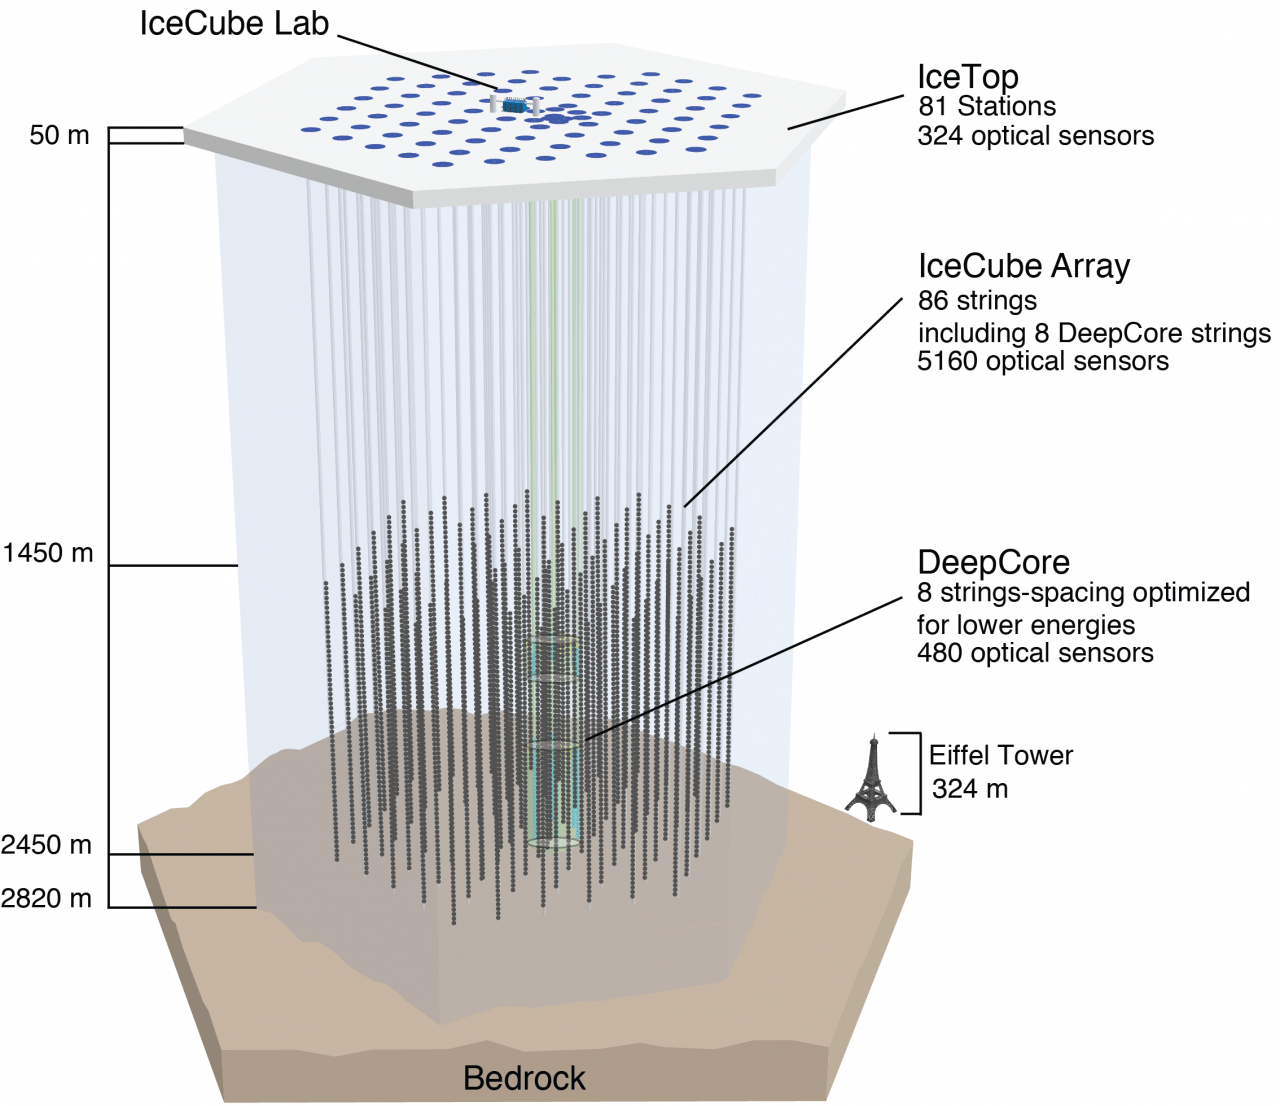
\includegraphics{figures/icecube/IceCubeArray_slim.png}
	\caption{An overview of the IceCube detector}
	\label{fig:ic_detector}
\end{figure}

\subsubsection{DeepCore}
The remaining 8 strings that are not part of the hexagonal grid are located near the center of the IceCube detector and form the \emph{DeepCore} sub-array\sidecite{DeepCore}.
The DOMs on the DeepCore strings have a higher quantum efficiency than those in the rest of the detector and are placed more closely together to lower the minimum energy threshold for neutrino observations to a few GeV.
Of the 60 DOMs on each DeepCore string, 50 are placed at depths between 2100~m and 2500~m, where the ice is the most transparent compared to the rest of the IceCube's volume (see also the side band in the bottom panel of Figure~\ref{fig:icecube-schematic}).
Together with 7 strings from the in-ice array, the DeepCore strings instrument the DeepCore 20~MT \emph{fiducial volume} as shown in the upper panel of Figure~\ref{fig:icecube-schematic}.
The remaining 10 DOMs are located at depths between 1750~m and 1850~m and are used as a veto cap to reject atmospheric muons entering the detector directly from above.
In addition, the larger hexagonal IceCube array also serves as a veto for observations inside the DeepCore fiducial volume.
\begin{figure}
    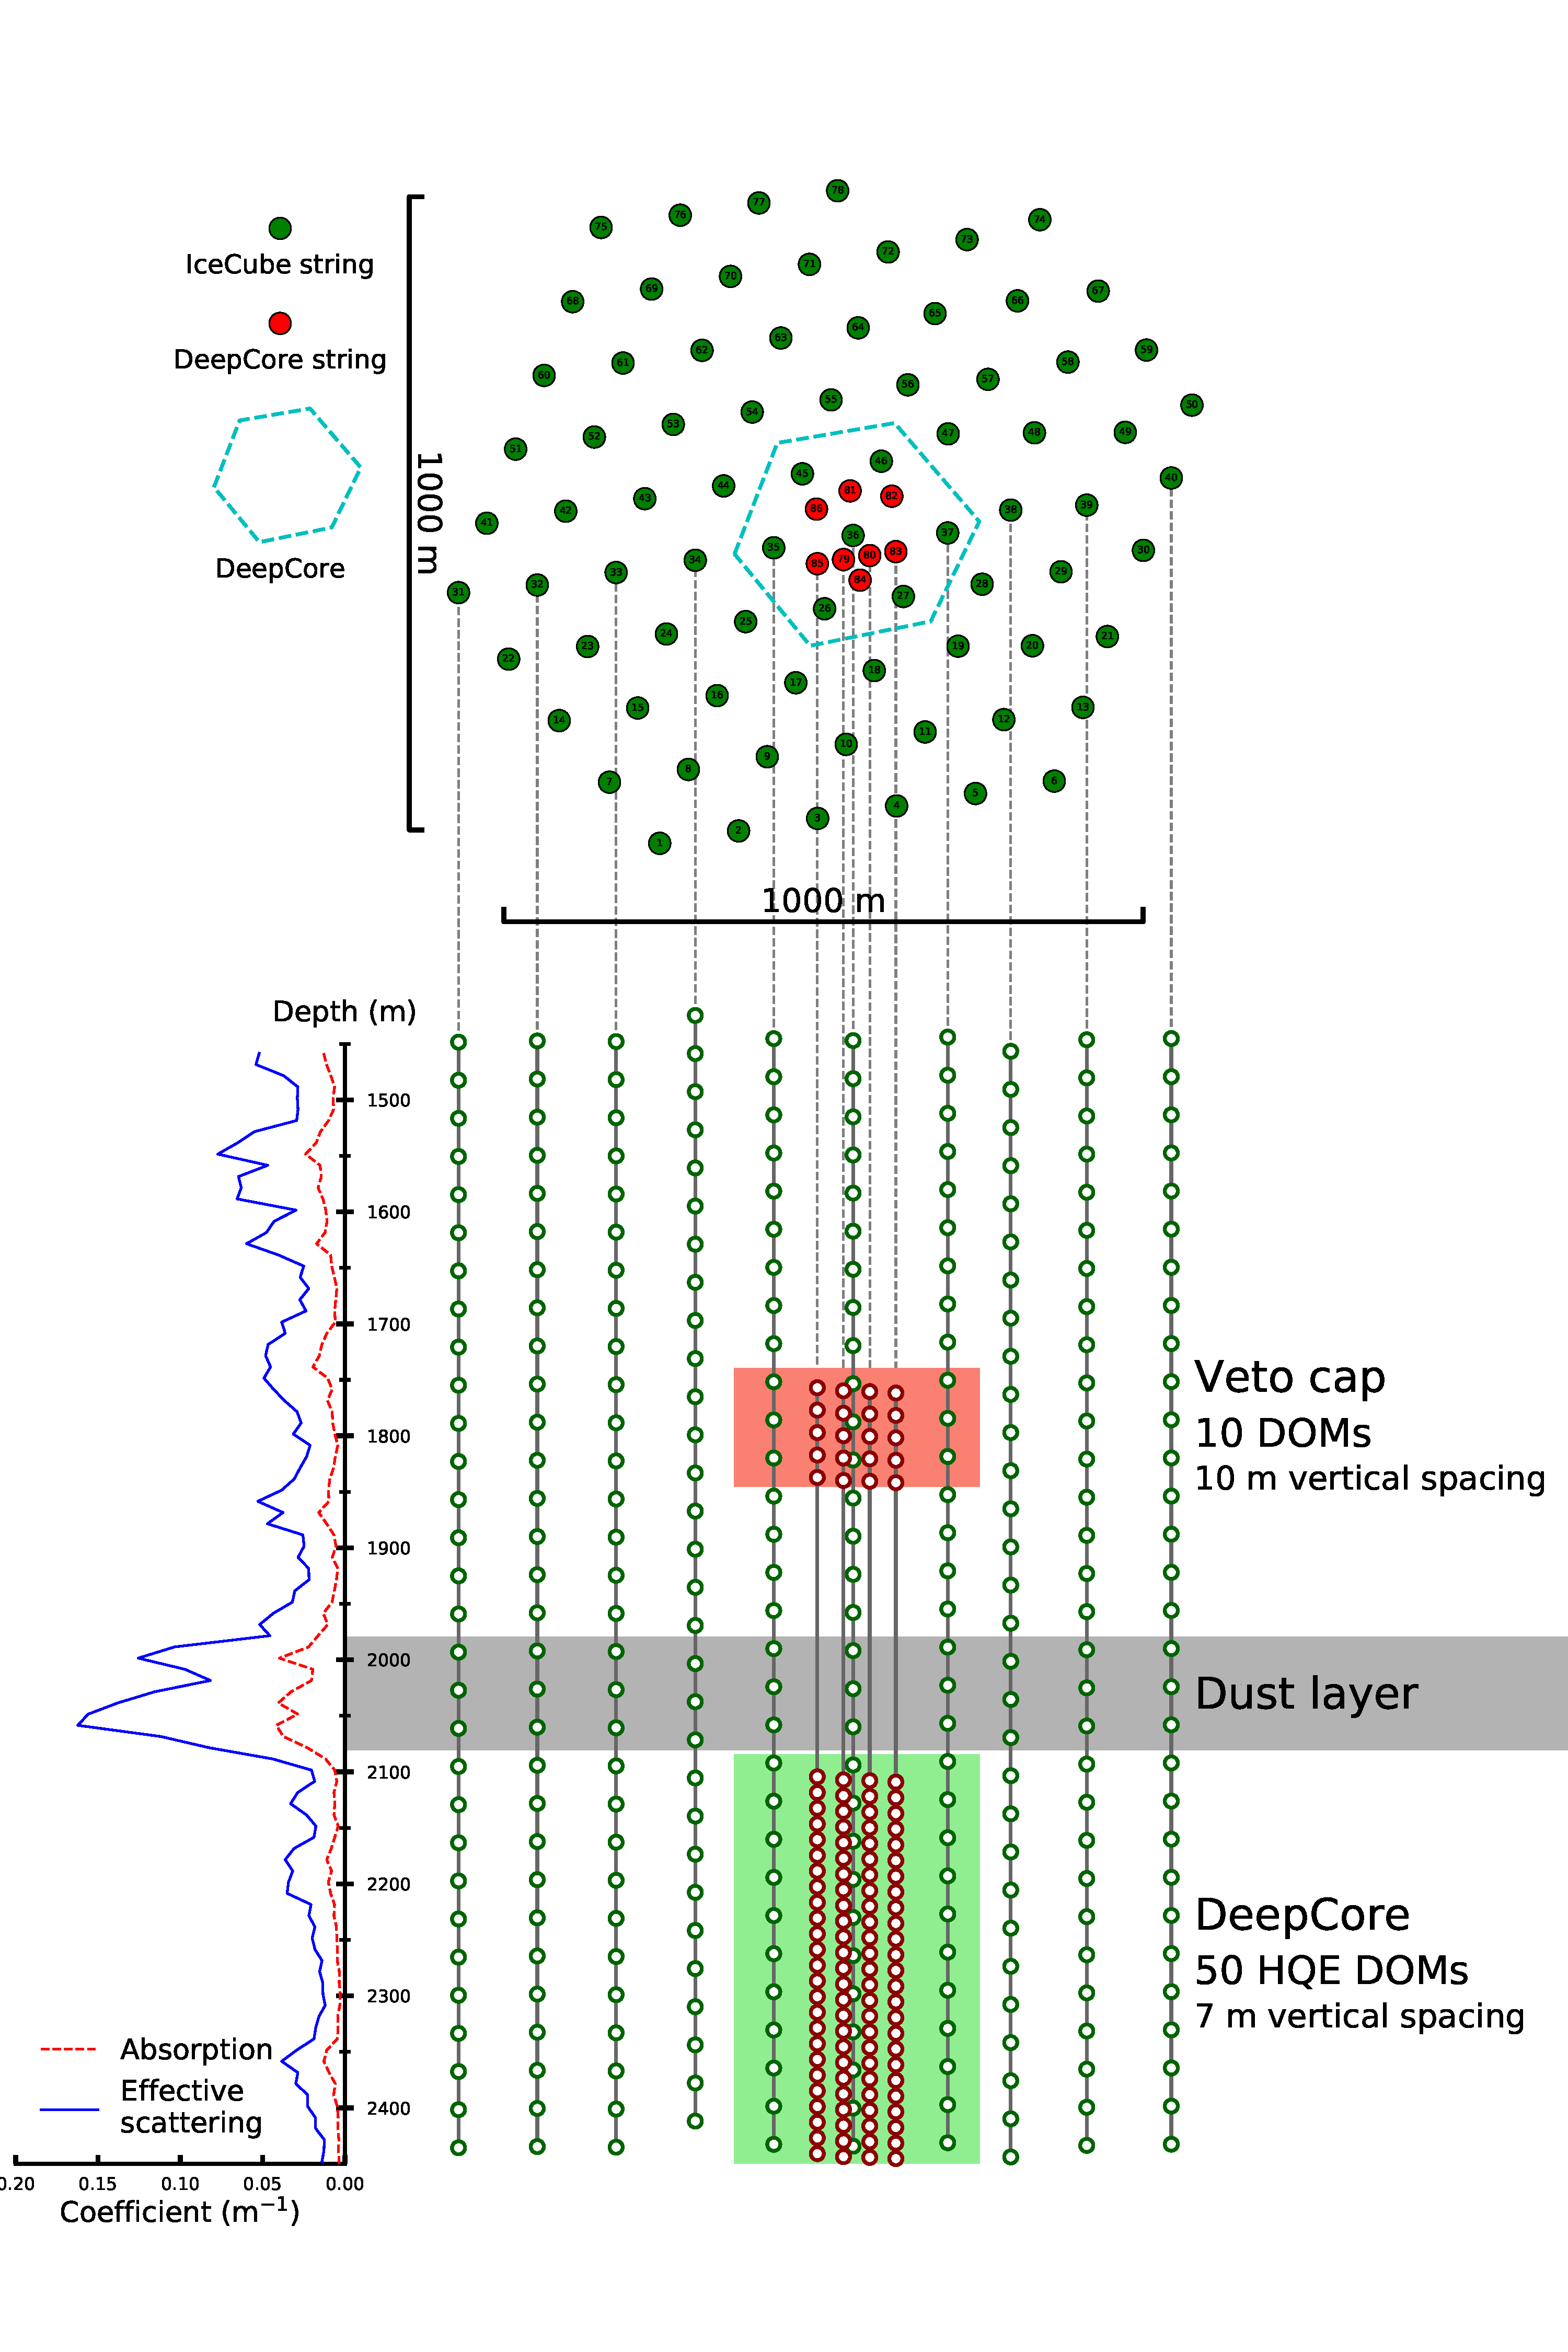
\includegraphics[width=0.9\linewidth]{figures/icecube/DeepCore_geometry.pdf}
    \caption{Schematic view of the IceCube detector as seen from the top (upper panel) and the side(lower panel). The DeepCore fiducial volume is indicated by the hexagon in the upper panel and the green shaded area in the bottom panel. The side-band on the lower panel shows the scattering and absorption coefficients as a function of depth.}
    \label{fig:icecube-schematic}
\end{figure}

\subsection{IceTop}

In addition to the in-ice array, IceCube also contains a surface array called \emph{IceTop}, consisting of 81 stations spread across an area of 1~km$^2$ that is used to detect muons from air showers.
It is typically used as a veto against atmospheric muons, but also functions as a detector in its own right measuring the spectrum and composition of cosmic particles.
%TODO: citation
However, it is not relevant to the measurement presented in this thesis.

\subsection{Digital Optical Modules}
\label{sec:dom-daq}
The Cherenkov radiation produced by charged particles in the ice is detected and digitized by Digital Optical Modules (DOMs).
Each module consists of a photo-multiplier tube (PMT)\sidecite{Abbasi_2010} and electronics housed in a transparent, spherical glass vessel that can withstand the enormous pressure below a water column of 2.5~km\cite{icecube_detector_17}.
They are each held in place by a harness attached to chains that allows the string cable to pass beside the DOM as shown in \reffig{dom-cable-assembly}.
\begin{marginfigure}[*-20]
    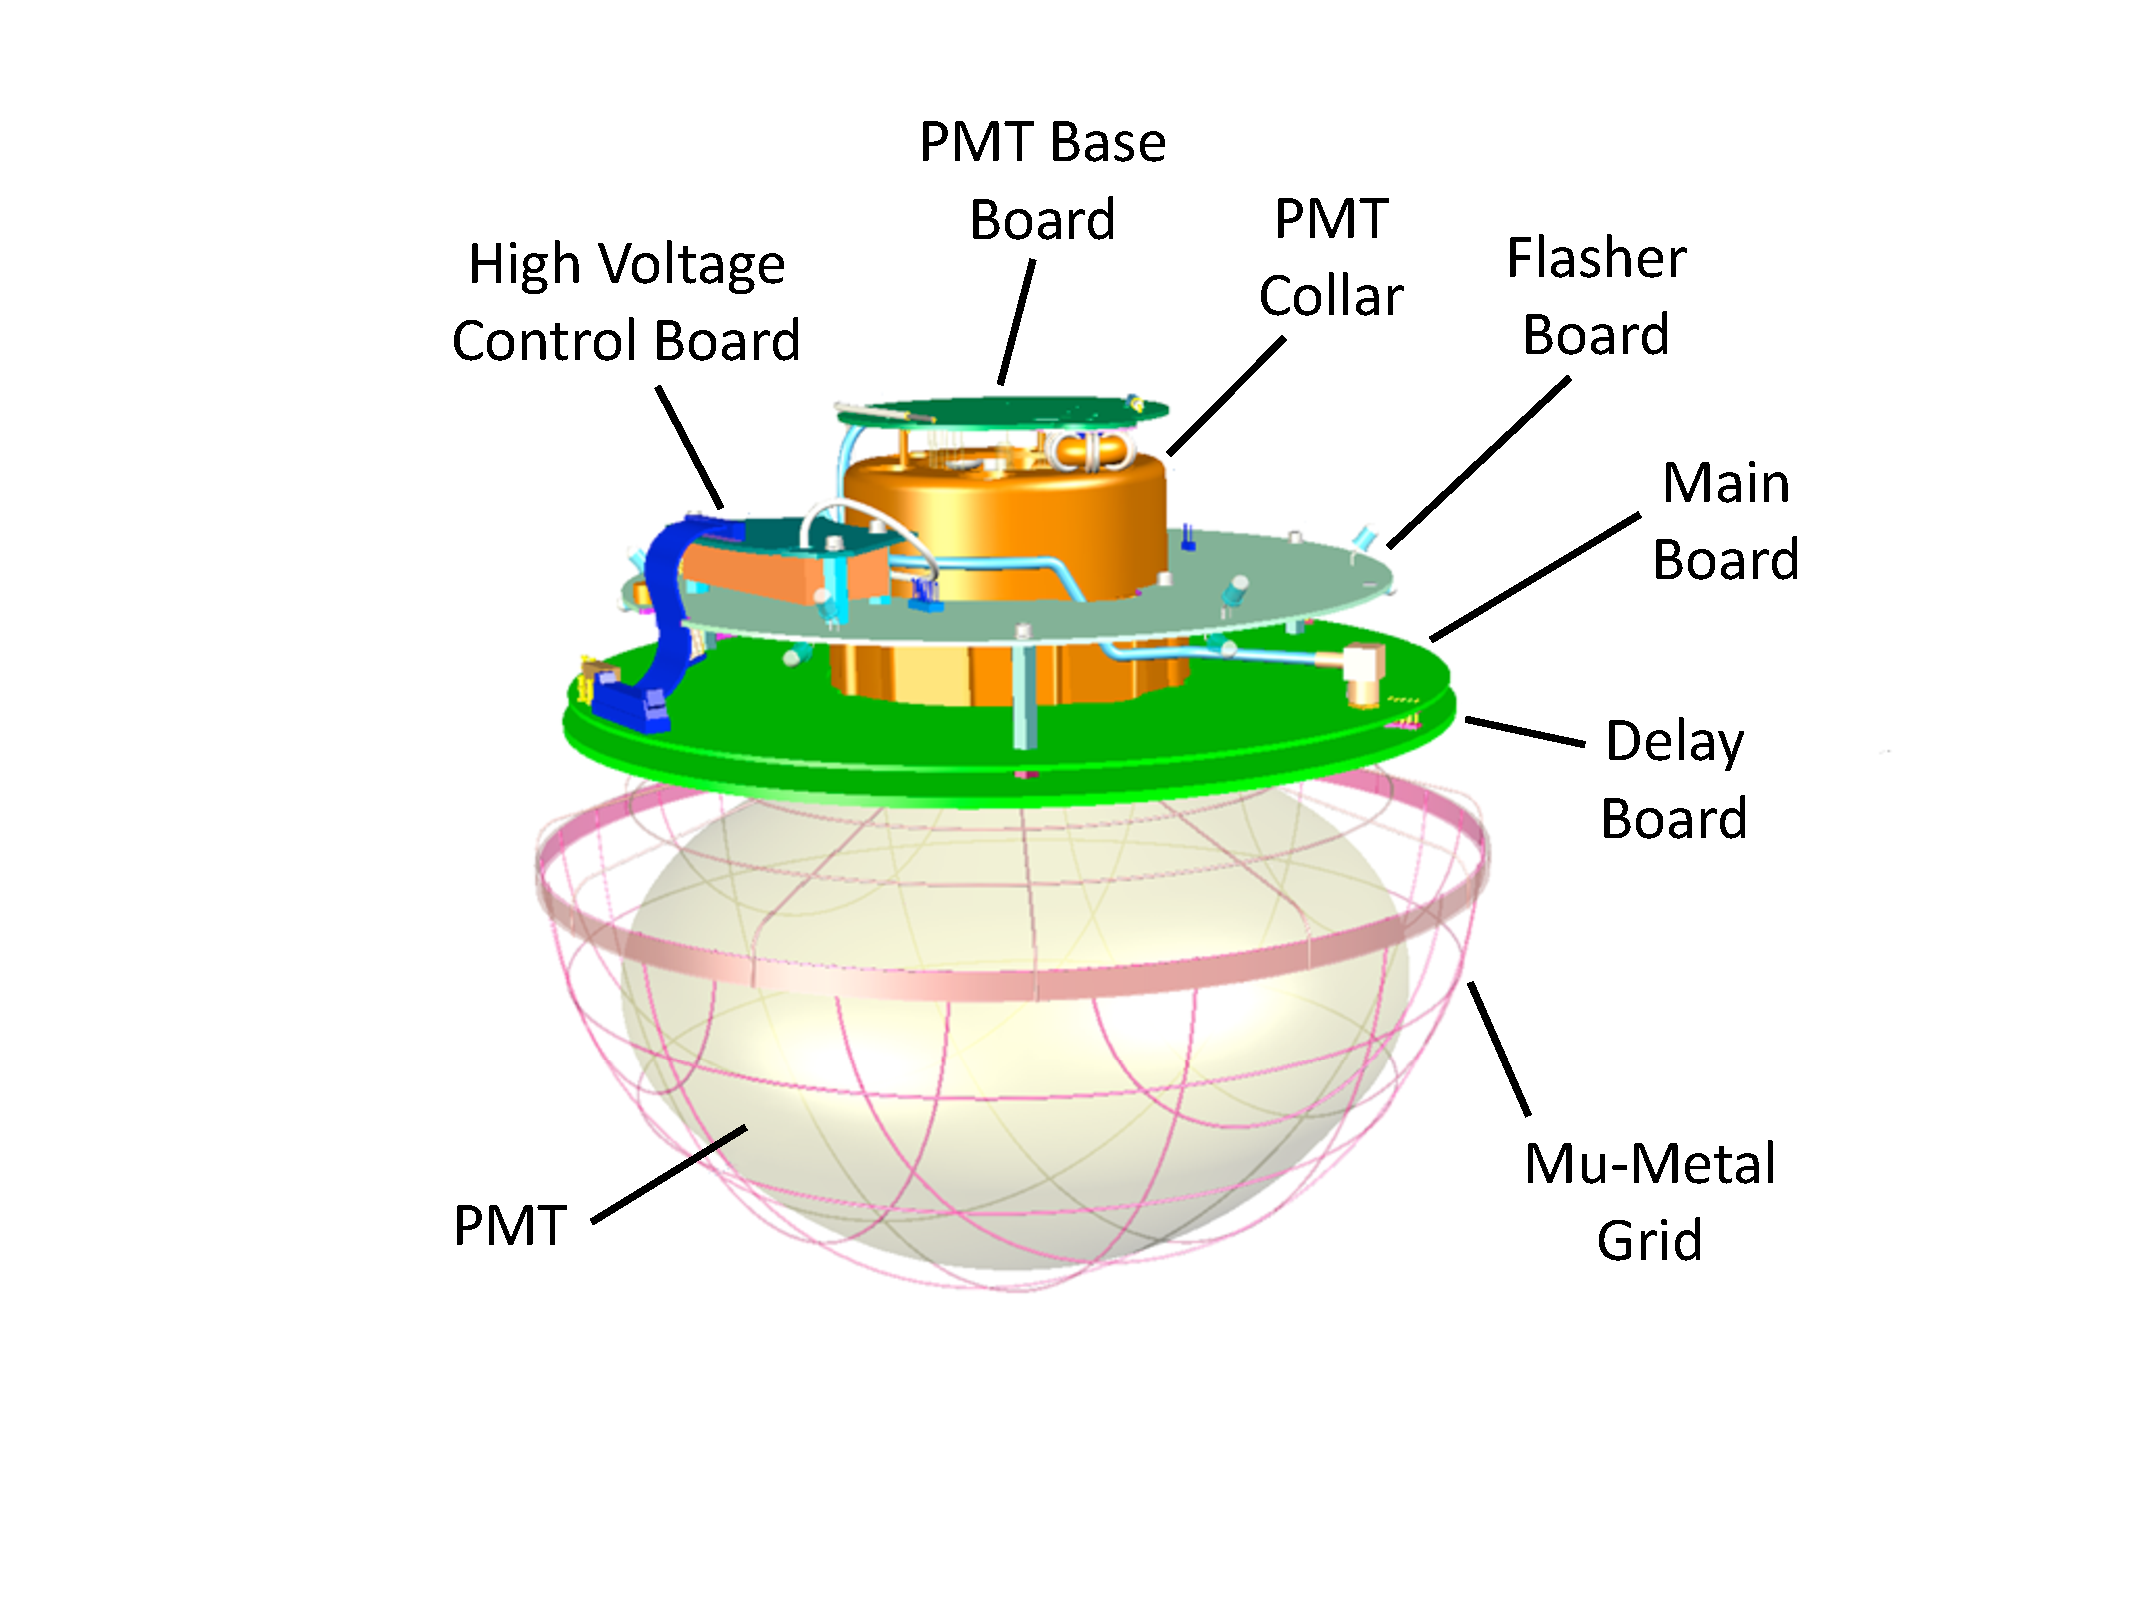
\includegraphics[width=\textwidth]{figures/icecube/domfig1a-DOM3DModel.pdf}
    \caption{Schematic of a DOM, taken from \cite{icecube_detector_17}.}
    \label{fig:dom-schematic}
\end{marginfigure}
\begin{marginfigure}
    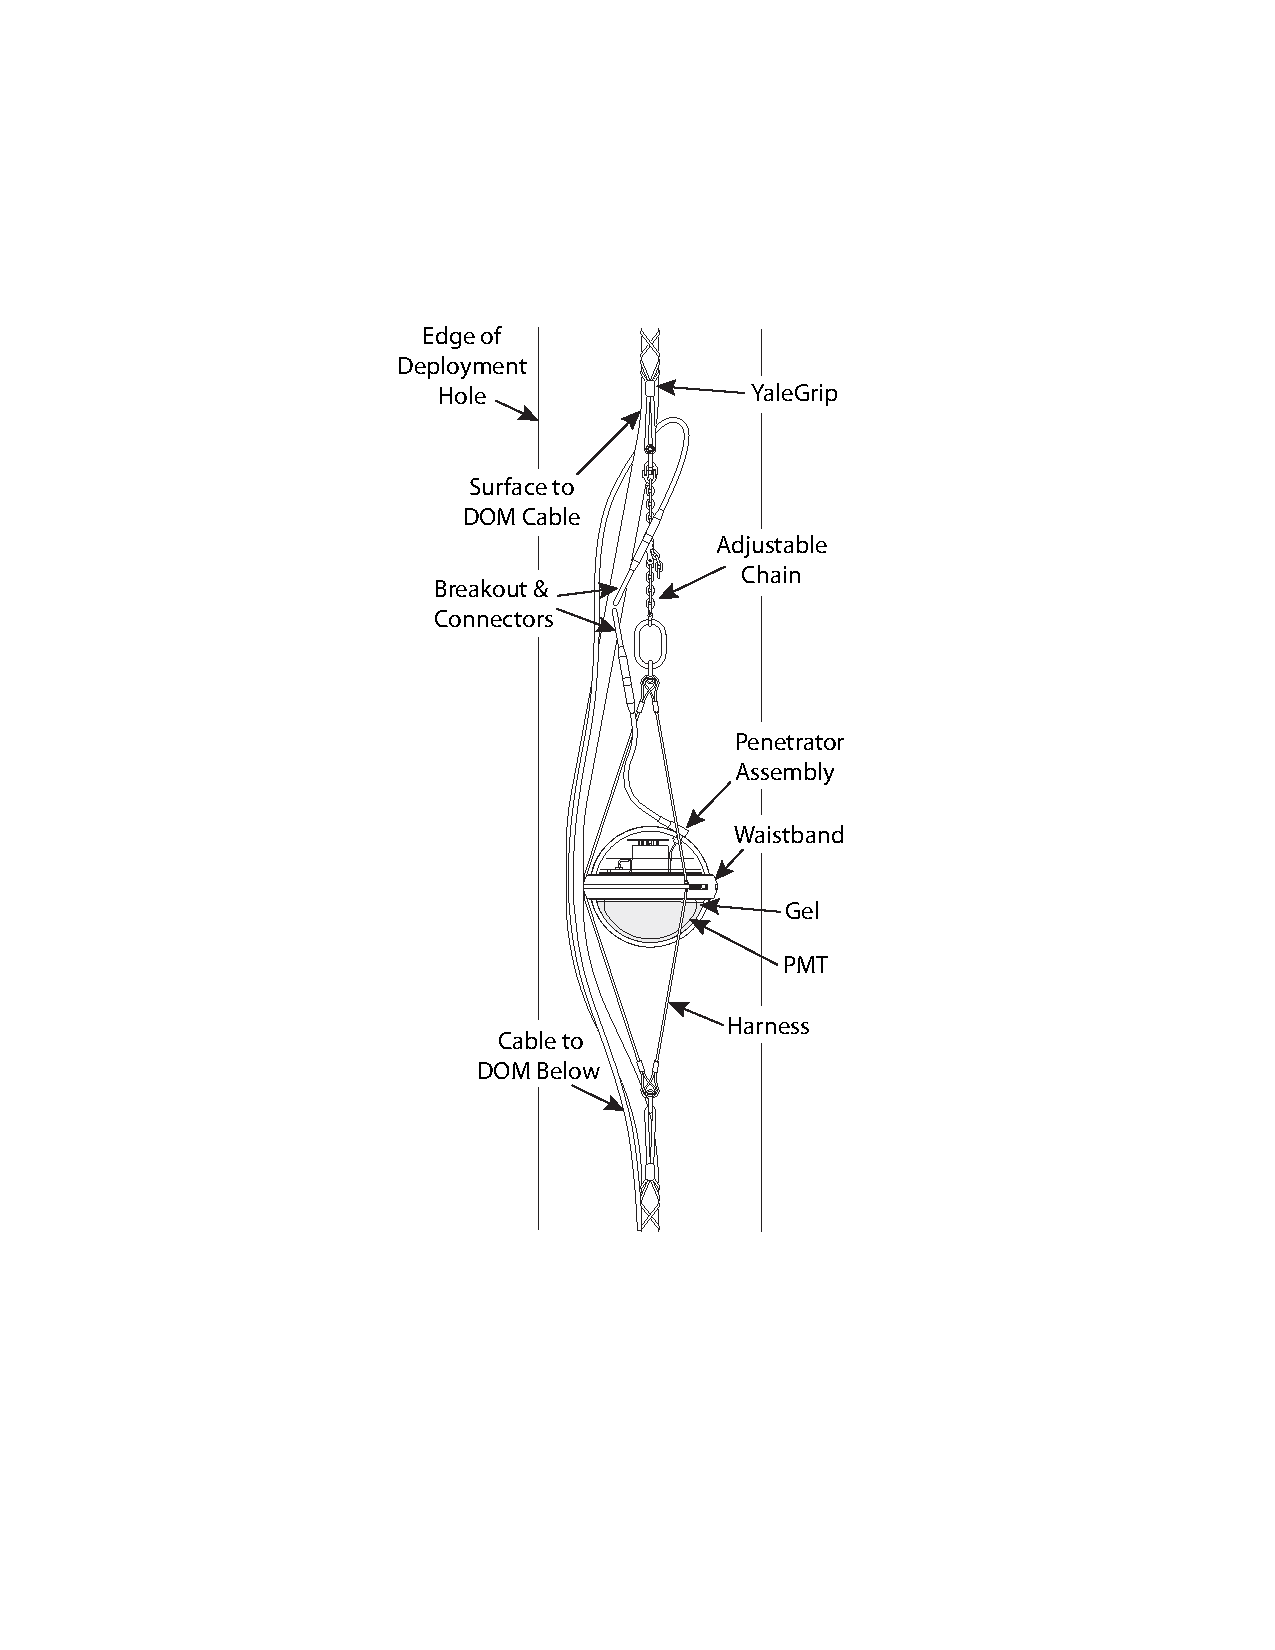
\includegraphics[width=\textwidth]{figures/icecube/domfig2a-CableAssembly.pdf}
    \caption{Schematic of the cable assembly of a DOM. Figure taken from \cite{icecube_detector_17}.}
    \label{fig:dom-cable-assembly}
\end{marginfigure}
The PMTs have a diameter of 10 inches and are sensitive to photons with wavelengths between 300~nm and 650~nm, with a maximum quantum efficiency of about 25\% at 390~nm.
Inside the DeepCore array, the peak efficiency reaches 34\%.
They are shielded from external magnetic fields with a mu-metal grid as shown in the schematic in Figure~\ref{fig:dom-schematic}.
The voltage at the PMT is measured and digitized by the on-board electronics\sidecite{icecube_daq} of the DOM in two separate readouts that are activated when the measured voltage rises above the equivalent of 0.25 photo-electrons (PE).
The first readout is the \emph{fast Analog-Digital Converter (fADC)} and measures the waveform continuously at a rate of 40~MHz.
The second readout, the \emph{Analog Transient Waveform Digitizer (ATWD)}, records the PMT voltage at a rate of 300~MHz in three channels with different gain levels to ensure that a large range\todo{what range?} of voltages can be recorded without saturation of the output.
The readout frequency of the ATWD is too high to be directly digitized and sent to the surface.
Instead, the ATWD voltage readout is buffered in 128 analog capacitors, corresponding to a readout time of $\sim$420~ns.
The buffered voltages are only digitized when at least one of the nearest or next-to-nearest DOMs on the same string also measures a signal within a 1~$\mu$s time window, which is referred to as the \emph{hard local coincidence (HLC)} condition.
The recorded waveforms are sent to the ICL on the surface, where they are compressed by applying the \emph{wavedeform} algorithm\sidecite{ic_spe_20}.
The output of this algorithm are reconstructed times and charges of single photo-electrons, which are taken as input by all further data processing steps described in section~\ref{sec:data-processing}.

The DOMs also contain a flasher board with 12 LEDs that can be used to emit pulsed light for the purpose of \emph{in-situ} detector calibration during special \emph{flasher runs} of the detector.
During such runs, the charge and time distributions of the observed pulses in the DOMs in response to the LED flashes are measured.
Since the light is emitted at known locations and at known times, the measured distributions allow inference on the absorption and scattering properties of the ice.
Because the total amplitude of the emitted light is less well known, this calibration method is less well suited for calibrating the total optical efficiency of the DOMs.
Instead, this property of the detector is calibrated more accurately from measurements of minimally-ionizing atmospheric muons, for which the energy loss is well known.


\section{Propagation of particles in ice}
\label{sec:particle-interactions}
Neutrinos interacting with the ice mostly interact via Deep Inelastic Scattering (DIS), creating muons, electromagnetic showers, and hadronic showers, depending on the flavor of the neutrino and interaction type.
The secondary particles produced by those interactions travel through the ice at highly relativistic velocities and lose energy primarily through ionization, bremsstrahlung, pair production and photo-nuclear interactions.
The fraction that each of these mechanisms contributes to the total energy loss of the particle depends on the type of particle and its energy.
When they are electrically charged, they also give off Cherenkov radiation that is then measured by IceCube.

\subsection{Cherenkov Effect}

The IceCube Neutrino Observatory relies entirely on the Cherenkov effect\sidecite{PhysRev.52.378} to detect particle interactions.
It is created by any electrically charged particle travelling through a transparent medium with velocities faster than the speed of light in that medium, $c/n$, where $n$ is the refractive index of the medium.
This produces a cone of light moving with the particle similar to a super-sonic shock that is generated by an object travelling through a gas at a velocity above the speed of sound.
The effect can be most easily understood according to Huygen's principle as a superposition of spherical light emissions that are produced every time that the particle displaces the charges in the dielectric medium in its closest vicinity, as shown in Figure~\ref{fig:cherenkov-sketch}.
When the particle is over-taking its own light emissions, they overlap coherently and form a conical light front as illustrated in the bottom panel of Figure~\ref{fig:cherenkov-sketch}.
\begin{marginfigure}[*-20]
    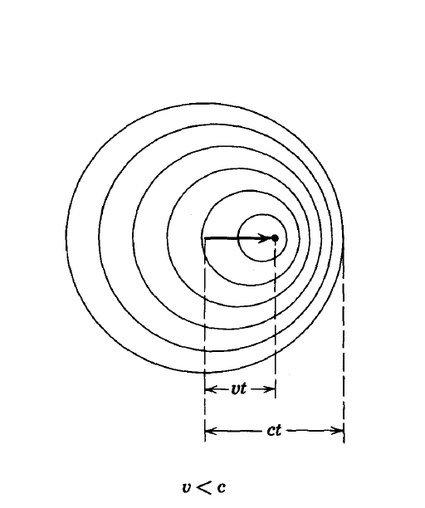
\includegraphics[width=\textwidth]{figures/icecube/cherenkov/cherenkov_slow.jpeg}
    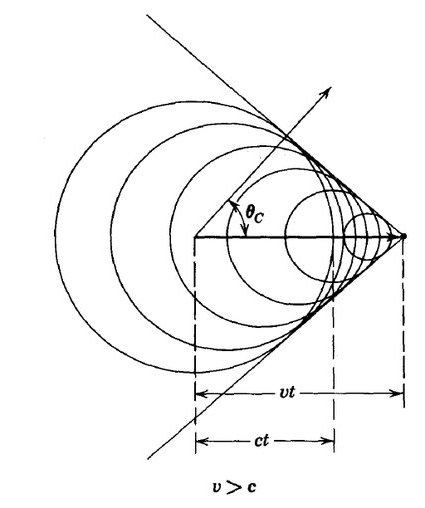
\includegraphics[width=\textwidth]{figures/icecube/cherenkov/cherenkov_fast.jpeg}
    \caption{An electrically charged particle emitting light while travelling below (upper panel) and above (lower panel) the speed of light in a medium. Image taken from \cite{jackson2012classical}.}
    \label{fig:cherenkov-sketch}
\end{marginfigure}
When the velocity of the particle is very close to the speed of light, as is the case for all (known) particles observable by IceCube, the opening angle of the cone only depends on the refractive index of the medium with
\begin{equation}
    \cos(\vartheta_c)=\frac{1}{\beta n}\;,
\end{equation}
where $n$ is the index of refraction and $\vartheta_c$ is the Cherenkov opening angle.

The frequency spectrum of the Cherenkov emissions of highly relativistic particles depends only on the charge of the particle, $q$, and the (wavelength-dependent) index of refraction, $n(\omega)$, and permeability, $\mu(\omega)$, of the medium.
The emitted energy per unit of distance and frequency is given by the Frank-Tamm-Equation\sidecite{Frank1937CoherentVR}\sidecite{Tamm1991}, which simplifies in the case of $v\approx c$ to
\begin{equation}
    \frac{\drm E}{\drm x \drm \omega}=\frac{q^2}{4\pi}\mu(\omega)\omega\left(1-\frac{1}{n^2(\omega)}\right)\,.
\end{equation}
The equation shows that the intensity of the Cherenkov emission generally increases with frequency, and indeed the strongest emissions are in the ultraviolet part of the spectrum.

\subsection{Muons}
\label{sec:muon-propagation}
At energies below 100~GeV, the dominant energy loss for muons is via ionization, and has only a weak dependence on energy.
Because the ionization loss is continuous and nearly constant, muons at these energies produce long, track-like signatures in the detector.
Above 100~GeV, the losses due to bremsstrahlung, pair production and photo-nuclear interactinos rise quickly in their amplitude and become dominant over ionization at $\sim$1~TeV.
The total average energy loss per unit distance, $\left<\drm E/\drm x\right>$, can be approximated combining all radiative energy losses (i.e.
all losses except for ionization) into one component and adding it to the ionization loss such that
\begin{equation}
    \left<-\frac{\drm E}{\drm x}\right> = a_I(E) + b_R(E)E\,,
\end{equation}
where $a_I(E)$ and $b_R(E)$ are slowly changing functions describing the ionization loss and the radiative losses, respectively\cite{muonstoppingpower}. For the energy ranges relevant for this work, the energy dependence of $a_I(E)$ and $b_R(E)$ is weak enough such that they can be approximated as constant numbers with $a_I(E)\approx 2\;\mathrm{MeV/cm}$ and $b_R(E)\approx3.4\times10^{-6}\;\mathrm{cm^{-1}}$\cite{muonstoppingpower}.
In this approximation, we can calculate the average length of a muon track, $\left<L\right>$, as a function of energy with
\begin{equation}
    \left<L\right>=\frac{1}{b_R}\log\left(\frac{b_R}{a_I}E + 1\right)\,,
\end{equation}
which gives an average travel distance of 50~m at 10~GeV and 460~m at 100~GeV.

\subsection{Electromagnetic Showers}
\label{sec:em-showers}
In contrast to muons, electrons and positrons lose their energy very quickly by emitting highly energetic photons due to bremsstrahlung.
The energy of the emitted photons is high enough that they spontaneously produce pairs of electrons and positrons.
This process is repeated until the electrons and positrons reach their critical energy, which is approximately 78~MeV in ice\sidecite{pdg}.
Below the critical energy, ionization takes over as the predominant mechanism of energy loss, which produces no new shower particles.
Another important quantity is the \emph{radiation length}, $X_0$, defined as the distance at which the energy of an electron is reduced to $\nicefrac{1}{e}$ of its initial energy via bremsstrahlung, which is 36~cm in ice\cite{pdg}.
The radiation length also determines the scale of the longitudinal development of the shower.
Expressing distances in units of radiation length as $t=x/X_0$, the shower intensity follows roughly a gamma distribution parametrized as
\begin{equation}
    \frac{\drm E}{\drm t} = E_0 b \frac{(bt)^{a-1}e^{-bt}}{\Gamma(a)}\;,
\end{equation}
where the parameters $a$ and $b$ need to be fit empirically\cite{pdg}.
Their values for electrons, positrons and photons interacting in ice have been determined from GEANT4\sidecite{geant4} shower simulations in\sidecite{RADEL2013102} to be
\begin{subequations}\label{eq:shower-params}
\begin{align}
    a &\approx 2.01 + 1.46 \log_{10}(E_0/\mathrm{GeV}),\; b\approx 0.63\; & (e^+,e^-), \label{eq:shower-params-1}\\
    a &\approx 2.84 + 1.34 \log_{10}(E_0/\mathrm{GeV}),\; b\approx 0.65\; & (\gamma).\label{eq:shower-params-2}
\end{align}
\end{subequations}
The shower reaches its maximum intensity at a distance of
\begin{equation}
    t_{\mathrm{max}}=\frac{a-1}{b}\;,
\end{equation}
which corresponds to a logarithmic growth of the size of the cascade according to \cref{eq:shower-params-1,eq:shower-params-2}.
The electrically charged components of the electromagnetic shower produce Cherenkov light, where the emissions peak at the Cherenkov angle since the secondary particles are emitted very close to the forward direction as shown in \reffig{cherenkov_angular_profile_cascade}.

\begin{marginfigure}
    \centering
    \tikzsetnextfilename{cascade_cherenkov_angular_dist}%
    % This file was created with tikzplotlib v0.10.1.
\begin{tikzpicture}

\definecolor{darkgray176}{RGB}{176,176,176}
\definecolor{darkorange25512714}{RGB}{255,127,14}
\definecolor{lightgray204}{RGB}{204,204,204}
\definecolor{steelblue31119180}{RGB}{31,119,180}

\begin{axis}[
height=0.8\linewidth,
legend cell align={left},
legend style={
  fill opacity=0.8,
  draw opacity=1,
  text opacity=1,
  at={(0.03,0.97)},
  anchor=north west,
  draw=lightgray204
},
log basis y={10},
minor xtick={},
minor ytick={0.0002,0.0003,0.0004,0.0005,0.0006,0.0007,0.0008,0.0009,0.002,0.003,0.004,0.005,0.006,0.007,0.008,0.009,0.02,0.03,0.04,0.05,0.06,0.07,0.08,0.09,0.2,0.3,0.4,0.5,0.6,0.7,0.8,0.9,2,3,4,5,6,7,8,9,20,30,40,50,60,70,80,90,200,300,400,500,600,700,800,900},
tick align=outside,
tick pos=left,
width=\linewidth,
x grid style={darkgray176},
xlabel={\(\scriptstyle \cos(\vartheta)\)},
xmajorgrids,
xmin=-1.1, xmax=1.1,
xtick style={color=black},
xtick={-1.5,-1,-0.5,0,0.5,1,1.5},
xticklabels={
\(\scriptstyle -1.5\),
\(\scriptstyle -1\),
\(\scriptstyle -0.5\),
\(\scriptstyle 0\),
\(\scriptstyle 0.5\),
\(\scriptstyle 1\),
\(\scriptstyle 1.5\)
},
y grid style={darkgray176},
ylabel={\(\scriptstyle \frac{1}{N}\frac{\mathrm{d}n}{\mathrm{d}\Omega}\;(\mathrm{sr^{-1}})\)},
ymajorgrids,
ymin=0.00198893054244642, ymax=1.79304902414132,
ymode=log,
ytick style={color=black},
ytick={0.0001,0.001,0.01,0.1,1,10,100},
yticklabels={
  \(\scriptstyle {10^{-4}}\),
  \(\scriptstyle {10^{-3}}\),
  \(\scriptstyle {10^{-2}}\),
  \(\scriptstyle {10^{-1}}\),
  \(\scriptstyle {10^{0}}\),
  \(\scriptstyle {10^{1}}\),
  \(\scriptstyle {10^{2}}\)
}
]
% \addlegendimage{empty legend}
% \addlegendentry{\hspace{-.6cm}\(\scriptstyle Primary particle\)}
\addplot [very thick, steelblue31119180]
table {%
-1 0.00270979570996691
-0.989949748743719 0.00274568176844791
-0.979899497487437 0.00278221344276632
-0.969849246231156 0.0028194051401974
-0.959798994974874 0.00285727165740652
-0.949748743718593 0.00289582819293
-0.939698492462312 0.002935090360122
-0.92964824120603 0.00297507420058719
-0.919597989949749 0.00301579619812029
-0.909547738693467 0.00305727329317443
-0.899497487437186 0.00309952289788118
-0.889447236180904 0.00314256291164658
-0.879396984924623 0.00318641173734847
-0.869346733668342 0.00323108829816169
-0.85929648241206 0.00327661205503912
-0.849246231155779 0.00332300302487796
-0.839195979899497 0.00337028179940208
-0.829145728643216 0.00341846956479283
-0.819095477386935 0.00346758812210248
-0.809045226130653 0.00351765990848599
-0.798994974874372 0.00356870801928906
-0.78894472361809 0.00362075623103195
-0.778894472361809 0.00367382902533086
-0.768844221105528 0.00372795161380099
-0.758793969849246 0.00378314996398742
-0.748743718592965 0.00383945082637282
-0.738693467336683 0.00389688176251318
-0.728643216080402 0.00395547117435602
-0.718592964824121 0.00401524833479813
-0.708542713567839 0.00407624341954317
-0.698492462311558 0.00413848754032286
-0.688442211055276 0.00420201277954891
-0.678391959798995 0.00426685222646659
-0.668341708542714 0.00433304001488506
-0.658291457286432 0.00440061136256355
-0.648241206030151 0.00446960261233712
-0.638190954773869 0.00454005127507061
-0.628140703517588 0.00461199607453446
-0.618090452261307 0.00468547699430147
-0.608040201005025 0.00476053532676948
-0.597989949748744 0.0048372137244211
-0.587939698492462 0.00491555625343831
-0.577889447236181 0.00499560844979658
-0.5678391959799 0.00507741737797107
-0.557788944723618 0.00516103169239503
-0.547738693467337 0.00524650170181962
-0.537688442211055 0.00533387943673301
-0.527638190954774 0.0054232187200069
-0.517587939698492 0.00551457524094897
-0.507537688442211 0.0056080066329506
-0.49748743718593 0.00570357255493209
-0.487437185929648 0.00580133477679948
-0.477386934673367 0.00590135726914189
-0.467336683417085 0.00600370629741217
-0.457286432160804 0.0061084505208506
-0.447236180904523 0.00621566109642723
-0.437185929648241 0.00632541178809819
-0.42713567839196 0.00643777908168967
-0.417085427135678 0.00655284230574558
-0.407035175879397 0.00667068375869704
-0.396984924623116 0.00679138884273666
-0.386934673366834 0.00691504620480722
-0.376884422110553 0.00704174788514251
-0.366834170854271 0.00717158947382927
-0.35678391959799 0.00730467027589214
-0.346733668341708 0.0074410934854396
-0.336683417085427 0.00758096636944745
-0.326633165829146 0.0077244004617986
-0.316582914572864 0.00787151176824312
-0.306532663316583 0.0080224209829917
-0.296482412060301 0.00817725371770887
-0.28643216080402 0.00833614074373032
-0.276381909547739 0.00849921824839105
-0.266331658291457 0.00866662810641917
-0.256281407035176 0.0088385181674243
-0.246231155778894 0.00901504256058975
-0.236180904522613 0.00919636201776539
-0.226130653266332 0.00938264421625311
-0.21608040201005 0.0095740641426814
-0.206030150753769 0.00977080447947795
-0.195979899497487 0.00997305601557417
-0.185929648241206 0.0101810180831098
-0.175879396984925 0.0103948990220547
-0.165829145728643 0.0106149166748261
-0.155778894472362 0.0108412989131575
-0.14572864321608 0.0110742841996714
-0.135678391959799 0.0113141221868181
-0.125628140703518 0.0115610743560839
-0.115577889447236 0.0118154147006228
-0.105527638190955 0.0120774304547576
-0.0954773869346733 0.0123474228741045
-0.085427135678392 0.0126257080704248
-0.0753768844221105 0.0129126179056865
-0.0653266331658291 0.0132085009502441
-0.0552763819095478 0.0135137235105104
-0.0452261306532663 0.0138286707320131
-0.035175879396985 0.0141537477843051
-0.0251256281407035 0.0144893811348354
-0.0150753768844221 0.0148360199195975
-0.00502512562814073 0.0151941374191663
0.00502512562814061 0.0155642326496143
0.0150753768844221 0.0159468320787846
0.0251256281407035 0.0163424914795012
0.035175879396985 0.0167517979325291
0.0452261306532664 0.0171753719934818
0.0552763819095476 0.0176138700394269
0.0653266331658291 0.0180679868126891
0.0753768844221105 0.0185384581813153
0.085427135678392 0.0190260641378932
0.0954773869346734 0.0195316320609182
0.105527638190955 0.0200560402657496
0.115577889447236 0.0206002218754172
0.125628140703518 0.0211651690451993
0.135678391959799 0.0217519375790622
0.14572864321608 0.022361651980798
0.155778894472362 0.0229955109881295
0.165829145728643 0.0236547936442626
0.175879396984925 0.0243408659685004
0.185929648241206 0.0250551882957267
0.195979899497488 0.0257993233640178
0.206030150753769 0.0265749452405507
0.21608040201005 0.0273838491886102
0.226130653266332 0.0282279625931581
0.236180904522613 0.0291093570794933
0.246231155778895 0.0300302619794334
0.256281407035176 0.030993079322741
0.266331658291457 0.03200040055884
0.276381909547739 0.0330550252460245
0.28643216080402 0.0341599819833132
0.296482412060302 0.0353185519050526
0.306532663316583 0.0365342951117703
0.316582914572864 0.0378110804744502
0.326633165829146 0.0391531193255863
0.336683417085427 0.040565003641884
0.346733668341709 0.0420517494338256
0.35678391959799 0.0436188461909371
0.366834170854271 0.0452723133940923
0.376884422110553 0.0470187653046993
0.386934673366834 0.0488654854842812
0.396984924623116 0.0508205127985405
0.407035175879397 0.0528927410327426
0.417085427135678 0.055092034710039
0.42713567839196 0.057429364287307
0.437185929648241 0.0599169646387465
0.447236180904523 0.0625685216719253
0.457286432160804 0.0653993931161115
0.467336683417085 0.0684268710625494
0.477386934673367 0.0716704958356979
0.487437185929648 0.0751524333921324
0.49748743718593 0.0788979319015025
0.507537688442211 0.0829358777746636
0.517587939698493 0.0872994776151978
0.527638190954774 0.0920271010294813
0.537688442211055 0.0971633308874874
0.547738693467337 0.102760283897193
0.557788944723618 0.108879287382879
0.5678391959799 0.115593031243989
0.577889447236181 0.122988362403445
0.587939698492462 0.131169960953129
0.597989949748744 0.140265246331153
0.608040201005025 0.15043103123486
0.618090452261307 0.16186271048248
0.628140703517588 0.17480721310861
0.638190954773869 0.189581691206729
0.648241206030151 0.20660122497593
0.658291457286432 0.226421210798552
0.668341708542714 0.249804685334967
0.678391959798995 0.277834184784676
0.688442211055276 0.312108201800071
0.698492462311558 0.355111292696392
0.708542713567839 0.410978453421262
0.718592964824121 0.487286890541685
0.728643216080402 0.60012697327905
0.738693467336683 0.793910321136359
0.748743718592965 1.3160586073339
0.758793969849246 1.02808069276863
0.768844221105528 0.705773104929006
0.778894472361809 0.551690720919282
0.78894472361809 0.455470028921774
0.798994974874372 0.388094231142621
0.809045226130653 0.337707570767511
0.819095477386935 0.298358445355108
0.829145728643216 0.266664676520879
0.839195979899497 0.240535857090921
0.849246231155779 0.218598677952748
0.85929648241206 0.199907969806359
0.869346733668342 0.183788893273284
0.879396984924623 0.169745057977341
0.889447236180904 0.157402218673429
0.899497487437186 0.146472295437764
0.909547738693467 0.13672956196271
0.919597989949749 0.127994411299455
0.92964824120603 0.120122001115478
0.939698492462312 0.112994133285036
0.949748743718593 0.106513332049104
0.959798994974874 0.100598450200823
0.969849246231156 0.0951813583735468
0.979899497487437 0.090204415681687
0.989949748743719 0.0856185130166524
1 0.0813815420878193
};
\addlegendentry{\(\scriptstyle e^-\)}
\addplot [very thick, darkorange25512714]
table {%
-1 0.00789216051649666
-0.989949748743719 0.00794087635636688
-0.979899497487437 0.00799046060080033
-0.969849246231156 0.00804093213801919
-0.959798994974874 0.00809231034956343
-0.949748743718593 0.00814461512551476
-0.939698492462312 0.00819786688026744
-0.92964824120603 0.00825208656886829
-0.919597989949749 0.00830729570394975
-0.909547738693467 0.00836351637328043
-0.899497487437186 0.0084207712579593
-0.889447236180904 0.00847908365128039
-0.879396984924623 0.00853847747829651
-0.869346733668342 0.00859897731611185
-0.85929648241206 0.00866060841493438
-0.849246231155779 0.00872339671992113
-0.839195979899497 0.00878736889385044
-0.829145728643216 0.00885255234065718
-0.819095477386935 0.00891897522986894
-0.809045226130653 0.00898666652198258
-0.798994974874372 0.0090556559948231
-0.78894472361809 0.00912597427092828
-0.778894472361809 0.00919765284600533
-0.768844221105528 0.00927072411850768
-0.758793969849246 0.00934522142038275
-0.748743718592965 0.00942117904904423
-0.738693467336683 0.00949863230062473
-0.728643216080402 0.00957761750456841
-0.718592964824121 0.00965817205962519
-0.708542713567839 0.00974033447131266
-0.698492462311558 0.00982414439091419
-0.688442211055276 0.00990964265608621
-0.678391959798995 0.00999687133315109
-0.668341708542714 0.0100858737611565
-0.658291457286432 0.0101766945977864
-0.648241206030151 0.0102693798672131
-0.638190954773869 0.0103639770099861
-0.628140703517588 0.0104605349350563
-0.618090452261307 0.0105591040740432
-0.608040201005025 0.0106597364378548
-0.597989949748744 0.0107624856757796
-0.587939698492462 0.0108674071371743
-0.577889447236181 0.0109745579358802
-0.5678391959799 0.0110839970175068
-0.557788944723618 0.0111957852297315
-0.547738693467337 0.0113099853957697
-0.537688442211055 0.0114266623911839
-0.527638190954774 0.0115458832242044
-0.517587939698492 0.0116677171197494
-0.507537688442211 0.0117922356073411
-0.49748743718593 0.0119195126131274
-0.487437185929648 0.0120496245562312
-0.477386934673367 0.0121826504496634
-0.467336683417085 0.0123186720060495
-0.457286432160804 0.0124577737484374
-0.447236180904523 0.0126000431264682
-0.437185929648241 0.0127455706382125
-0.42713567839196 0.0128944499579918
-0.417085427135678 0.0130467780705269
-0.407035175879397 0.0132026554117768
-0.396984924623116 0.013362186016856
-0.386934673366834 0.0135254776754425
-0.376884422110553 0.0136926420951192
-0.366834170854271 0.0138637950731175
-0.35678391959799 0.0140390566769668
-0.346733668341708 0.0142185514345872
-0.336683417085427 0.0144024085343986
-0.326633165829146 0.0145907620360627
-0.316582914572864 0.0147837510925123
-0.306532663316583 0.0149815201839753
-0.296482412060301 0.0151842193647459
-0.28643216080402 0.0153920045235134
-0.276381909547739 0.0156050376581157
-0.266331658291457 0.0158234871656503
-0.256281407035176 0.0160475281489437
-0.246231155778894 0.0162773427404552
-0.236180904522613 0.0165131204447723
-0.226130653266332 0.0167550585009444
-0.21608040201005 0.0170033622659962
-0.206030150753769 0.0172582456210662
-0.195979899497487 0.0175199314017323
-0.185929648241206 0.0177886518542055
-0.175879396984925 0.0180646491192131
-0.165829145728643 0.0183481757455348
-0.155778894472362 0.0186394952353194
-0.14572864321608 0.0189388826234856
-0.135678391959799 0.0192466250936987
-0.125628140703518 0.0195630226336309
-0.115577889447236 0.0198883887324402
-0.105527638190955 0.0202230511236558
-0.0954773869346733 0.0205673525769393
-0.085427135678392 0.0209216517424914
-0.0753768844221105 0.0212863240522157
-0.0653266331658291 0.0216617626821167
-0.0552763819095478 0.0220483795808203
-0.0452261306532663 0.022446606569557
-0.035175879396985 0.0228568965194424
-0.0251256281407035 0.0232797246124452
-0.0150753768844221 0.0237155896930427
-0.00502512562814073 0.0241650157182394
0.00502512562814061 0.0246285533143807
0.0150753768844221 0.0251067814500269
0.0251256281407035 0.025600309235087
0.035175879396985 0.0261097778574502
0.0452261306532664 0.0266358626695118
0.0552763819095476 0.0271792754382893
0.0653266331658291 0.0277407667742745
0.0753768844221105 0.0283211287557975
0.085427135678392 0.0289211977675074
0.0954773869346734 0.0295418575736295
0.105527638190955 0.0301840426489816
0.115577889447236 0.0308487417933436
0.125628140703518 0.0315370020577348
0.135678391959799 0.032249933014505
0.14572864321608 0.032988711406942
0.155778894472362 0.0337545862184264
0.165829145728643 0.0345488842060796
0.175879396984925 0.0353730159494754
0.185929648241206 0.0362284824714063
0.195979899497488 0.0371168824950634
0.206030150753769 0.0380399204104475
0.21608040201005 0.0389994150325696
0.226130653266332 0.0399973092452438
0.236180904522613 0.0410356806372771
0.246231155778895 0.0421167532529549
0.256281407035176 0.0432429105962605
0.266331658291457 0.0444167100487352
0.276381909547739 0.0456408988848156
0.28643216080402 0.0469184320965592
0.296482412060302 0.048252492272703
0.306532663316583 0.0496465118159931
0.316582914572864 0.0511041978289106
0.326633165829146 0.0526295600528103
0.336683417085427 0.0542269423109717
0.346733668341709 0.0559010579844757
0.35678391959799 0.0576570301440859
0.366834170854271 0.0595004370751213
0.376884422110553 0.0614373640703005
0.386934673366834 0.0634744625336283
0.396984924623116 0.0656190176441357
0.407035175879397 0.0678790260813921
0.417085427135678 0.0702632856277359
0.42713567839196 0.0727814988515182
0.437185929648241 0.075444393562777
0.447236180904523 0.0782638633461016
0.457286432160804 0.0812531322528268
0.467336683417085 0.0844269487270227
0.477386934673367 0.0878018151159875
0.487437185929648 0.0913962607705643
0.49748743718593 0.0952311689042153
0.507537688442211 0.099330170235027
0.517587939698493 0.103720120240028
0.527638190954774 0.108431681976416
0.537688442211055 0.113500043406718
0.547738693467337 0.118965807795903
0.557788944723618 0.124876109212345
0.5678391959799 0.131286024264284
0.577889447236181 0.138260378736104
0.587939698492462 0.145876088183355
0.597989949748744 0.154225231976222
0.608040201005025 0.163419152664381
0.618090452261307 0.173594017226095
0.628140703517588 0.18491850963698
0.638190954773869 0.197604710766709
0.648241206030151 0.211923886477276
0.658291457286432 0.228230096197278
0.668341708542714 0.246996774450726
0.678391959798995 0.26887589872466
0.688442211055276 0.294798880744473
0.698492462311558 0.32616049150544
0.708542713567839 0.36518484083375
0.718592964824121 0.41574694864329
0.728643216080402 0.48557899814055
0.738693467336683 0.594309602959545
0.748743718592965 0.835983791833013
0.758793969849246 0.710693050136147
0.768844221105528 0.546432769731992
0.778894472361809 0.456265851073738
0.78894472361809 0.395022749599503
0.798994974874372 0.349420179510256
0.809045226130653 0.313615587438124
0.819095477386935 0.284503587518325
0.829145728643216 0.260234102069794
0.839195979899497 0.239616407766554
0.849246231155779 0.221839941214909
0.85929648241206 0.206328850988604
0.869346733668342 0.192660020219313
0.879396984924623 0.180513958673293
0.889447236180904 0.169643916401901
0.899497487437186 0.159855667085849
0.909547738693467 0.150993826949325
0.919597989949749 0.142932331066801
0.92964824120603 0.135567640702552
0.939698492462312 0.128813795145942
0.949748743718593 0.122598739772099
0.959798994974874 0.116861556117663
0.969849246231156 0.111550341625584
0.979899497487437 0.10662056525917
0.989949748743719 0.102033776999246
1 0.0977565841356766
};
\addlegendentry{\(\scriptstyle \pi^+\)}
\addplot [black, dashed, forget plot]
table {%
0.75187969924812 0.00198893054244642
0.75187969924812 1.79304902414132
};
\end{axis}

\end{tikzpicture}


    \caption{Angular profile of the Cherenkov emission of an electromagnetic cascade ($e^-$) and a hadronic cascade ($\pi^+$) using the parametrization from \cite{RADEL2013102}.}
    \label{fig:cherenkov_angular_profile_cascade}
\end{marginfigure}

\subsection{Hadronic Showers}
\label{sec:had-showers}
As discussed in section~\ref{sec:neutrino-xsec}, neutrino interactions above 10~GeV happen almost exclusively via Deep-Inelastic Scattering (DIS).
These interactions always produce a hadronic cascade in addition to any leptons in the final state.
Hadronic cascades are also the only visible part of the final state of neutral-current interactions.
Hadrons (mostly Pions) that are produced in neutrino-nucleon interactions interact strongly with the surrounding ice to create secondary particles and then decay to form additional photons and leptons.
Charged secondary particles produce Cherenkov radiation, while neutral secondary particles are invisible to the detector.
Because part of the energy deposited in a hadronic shower is not measurable, the inherent uncertainty on the true energy of the primary particle that initiated the interaction is larger.
The average visible electromagnetic fraction of a hadronic shower can be parametrized\cite{RADEL2013102} as a function of the initial energy with
\begin{equation}
    F(E_0) = 1 - (1-f_0)\left(\frac{E_0}{E_s}\right)^{-m}
\end{equation}
with a variance of
\begin{equation}
    \sigma_F(E_0) = \sigma_0 \log(E_0)^{-\gamma}\,.
\end{equation}
The parameters $f_0$, $E_s$, $m$, $\sigma_0$, and $\gamma$ are fit to GEANT4 simulation results for hadronic showers induced by different primary particles in\cite{RADEL2013102}.
The Cherenkov emissions from the charged components of the shower still peak around the Cherenkov angle as they do for electromagnetic showers, but the emission profile is more smeared out due to the larger variations in particle kinematics as can be seen in figure~\ref{fig:cherenkov_angular_profile_cascade} for the example of a shower induced by a pion.


\section{Particle Signatures in IceCube}
\label{sec:particle-signatures}
All particle signatures in IceCube can be approximated as being combinations of compact \emph{cascades} that are produced by hadronic and electromagnetic showers (see section~\ref{sec:had-showers} and \ref{sec:em-showers}), and elongated \emph{tracks} that are only produced by muons travelling through the detector.

\subsection{Neutrinos}

At energies above 10~GeV, nearly all neutrino interactions are due to Deep Inelastic Scattering (DIS) and therefore always produce at least a hadronic cascade originating at the interaction vertex.
In Neutral-Current (NC) interactions, this hadronic cascade is the only visible part of the interaction.
Charged-current (CC) interactions also produce a lepton of the same flavor as the primary neutrino.
For electron-neutrinos, this creates an electromagnetic (EM) shower that originates at the interaction vertex.
While the direction of the EM shower and the hadronic shower might not be exactly the same, they are in practice not distinguishable by the detector and can therefore be approximated as a single cascade-like signature.
Since the directions of the particles that make up a shower are randomly distributed with a strong bias towards the direction of the primary neutrino, the angular profile of the light emission of a cascade follows a smeared Cherenkov emission profile.
At distances of several scattering lengths ($L_s\approx25\;\mathrm{m}$), this emission profile averages out and the cascade can be approximated as a single point emitting light uniformly in all directions.
The left panel of figure~\ref{fig:idealized_signatures} shows the detector response of such an idealized, perfectly symmetric cascade event.
As described in \refsec{antineutrino-scattering}, the only distinction between the interactions of neutrinos and antineutrinos is a difference in their cross-section as a function of the inelasticity that is due to their spin configuration.
It is therefore impossible to distinguish between the two signatures on an event-by-event basis, even though statistical inferences about the relative distributions of neutrinos and antineutrinos can be made given a sufficiently large population\sidecite{lasse-inelasticity}.
\begin{figure}
    \centering
    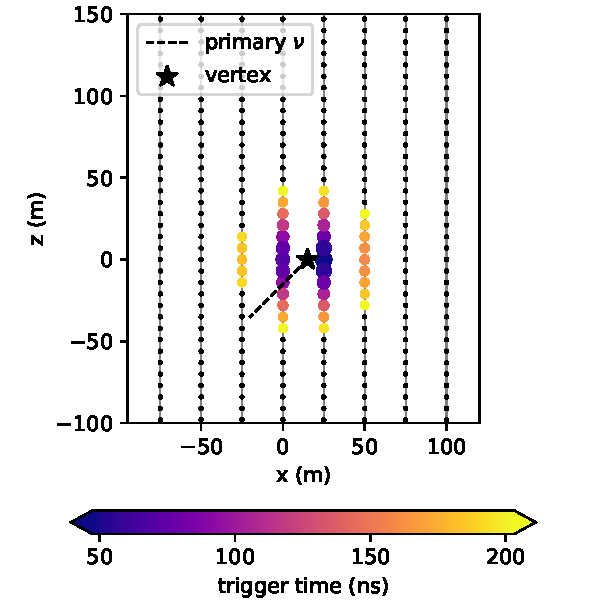
\includegraphics[width=0.49\textwidth]{figures/icecube/eventviews/idealized_cascade_view.pdf}
    \hfill
    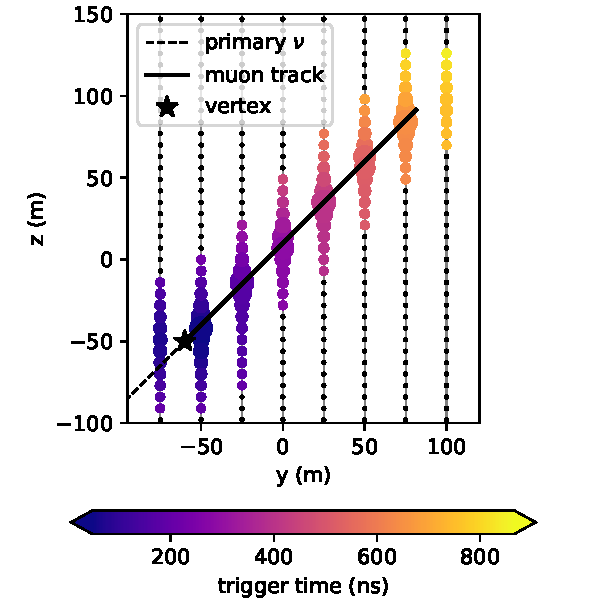
\includegraphics[width=0.49\textwidth]{figures/icecube/eventviews/idealized_track_view.pdf}
    \caption{An idealized cascade event (left) and starting track event (right) seen from the side. Each DOM that has received light is highlighted with a colored bubble, where the size is proportional the total charge seen by the DOM and the color indicates the time of the hits relative to the time at which the neutrino interaction happened.}
    \label{fig:idealized_signatures}
\end{figure}

% \begin{marginfigure}
%     \centering
%     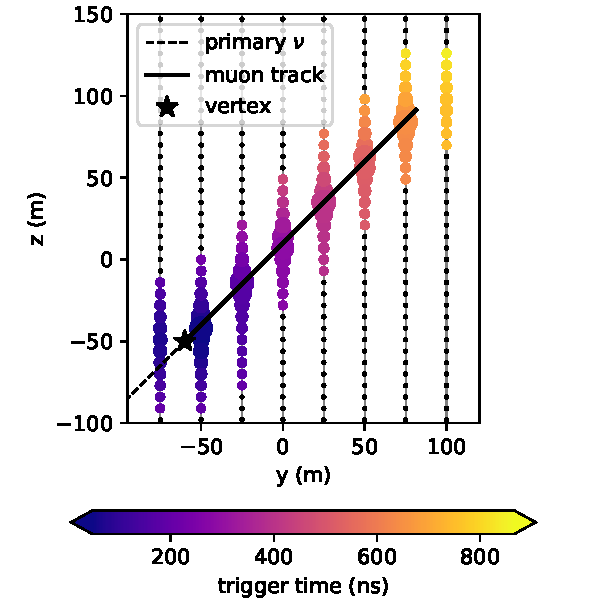
\includegraphics[width=\textwidth]{figures/icecube/eventviews/idealized_track_view.pdf}
%     \caption{An idealized \numucc-event seen from the side. Light is emitted uniformly from the interaction vertex as well as the endpoint of the track, and follows the Cherenkov cone along the track.}
%     \label{fig:idealized_track}
% \end{marginfigure}
% \begin{marginfigure}
%     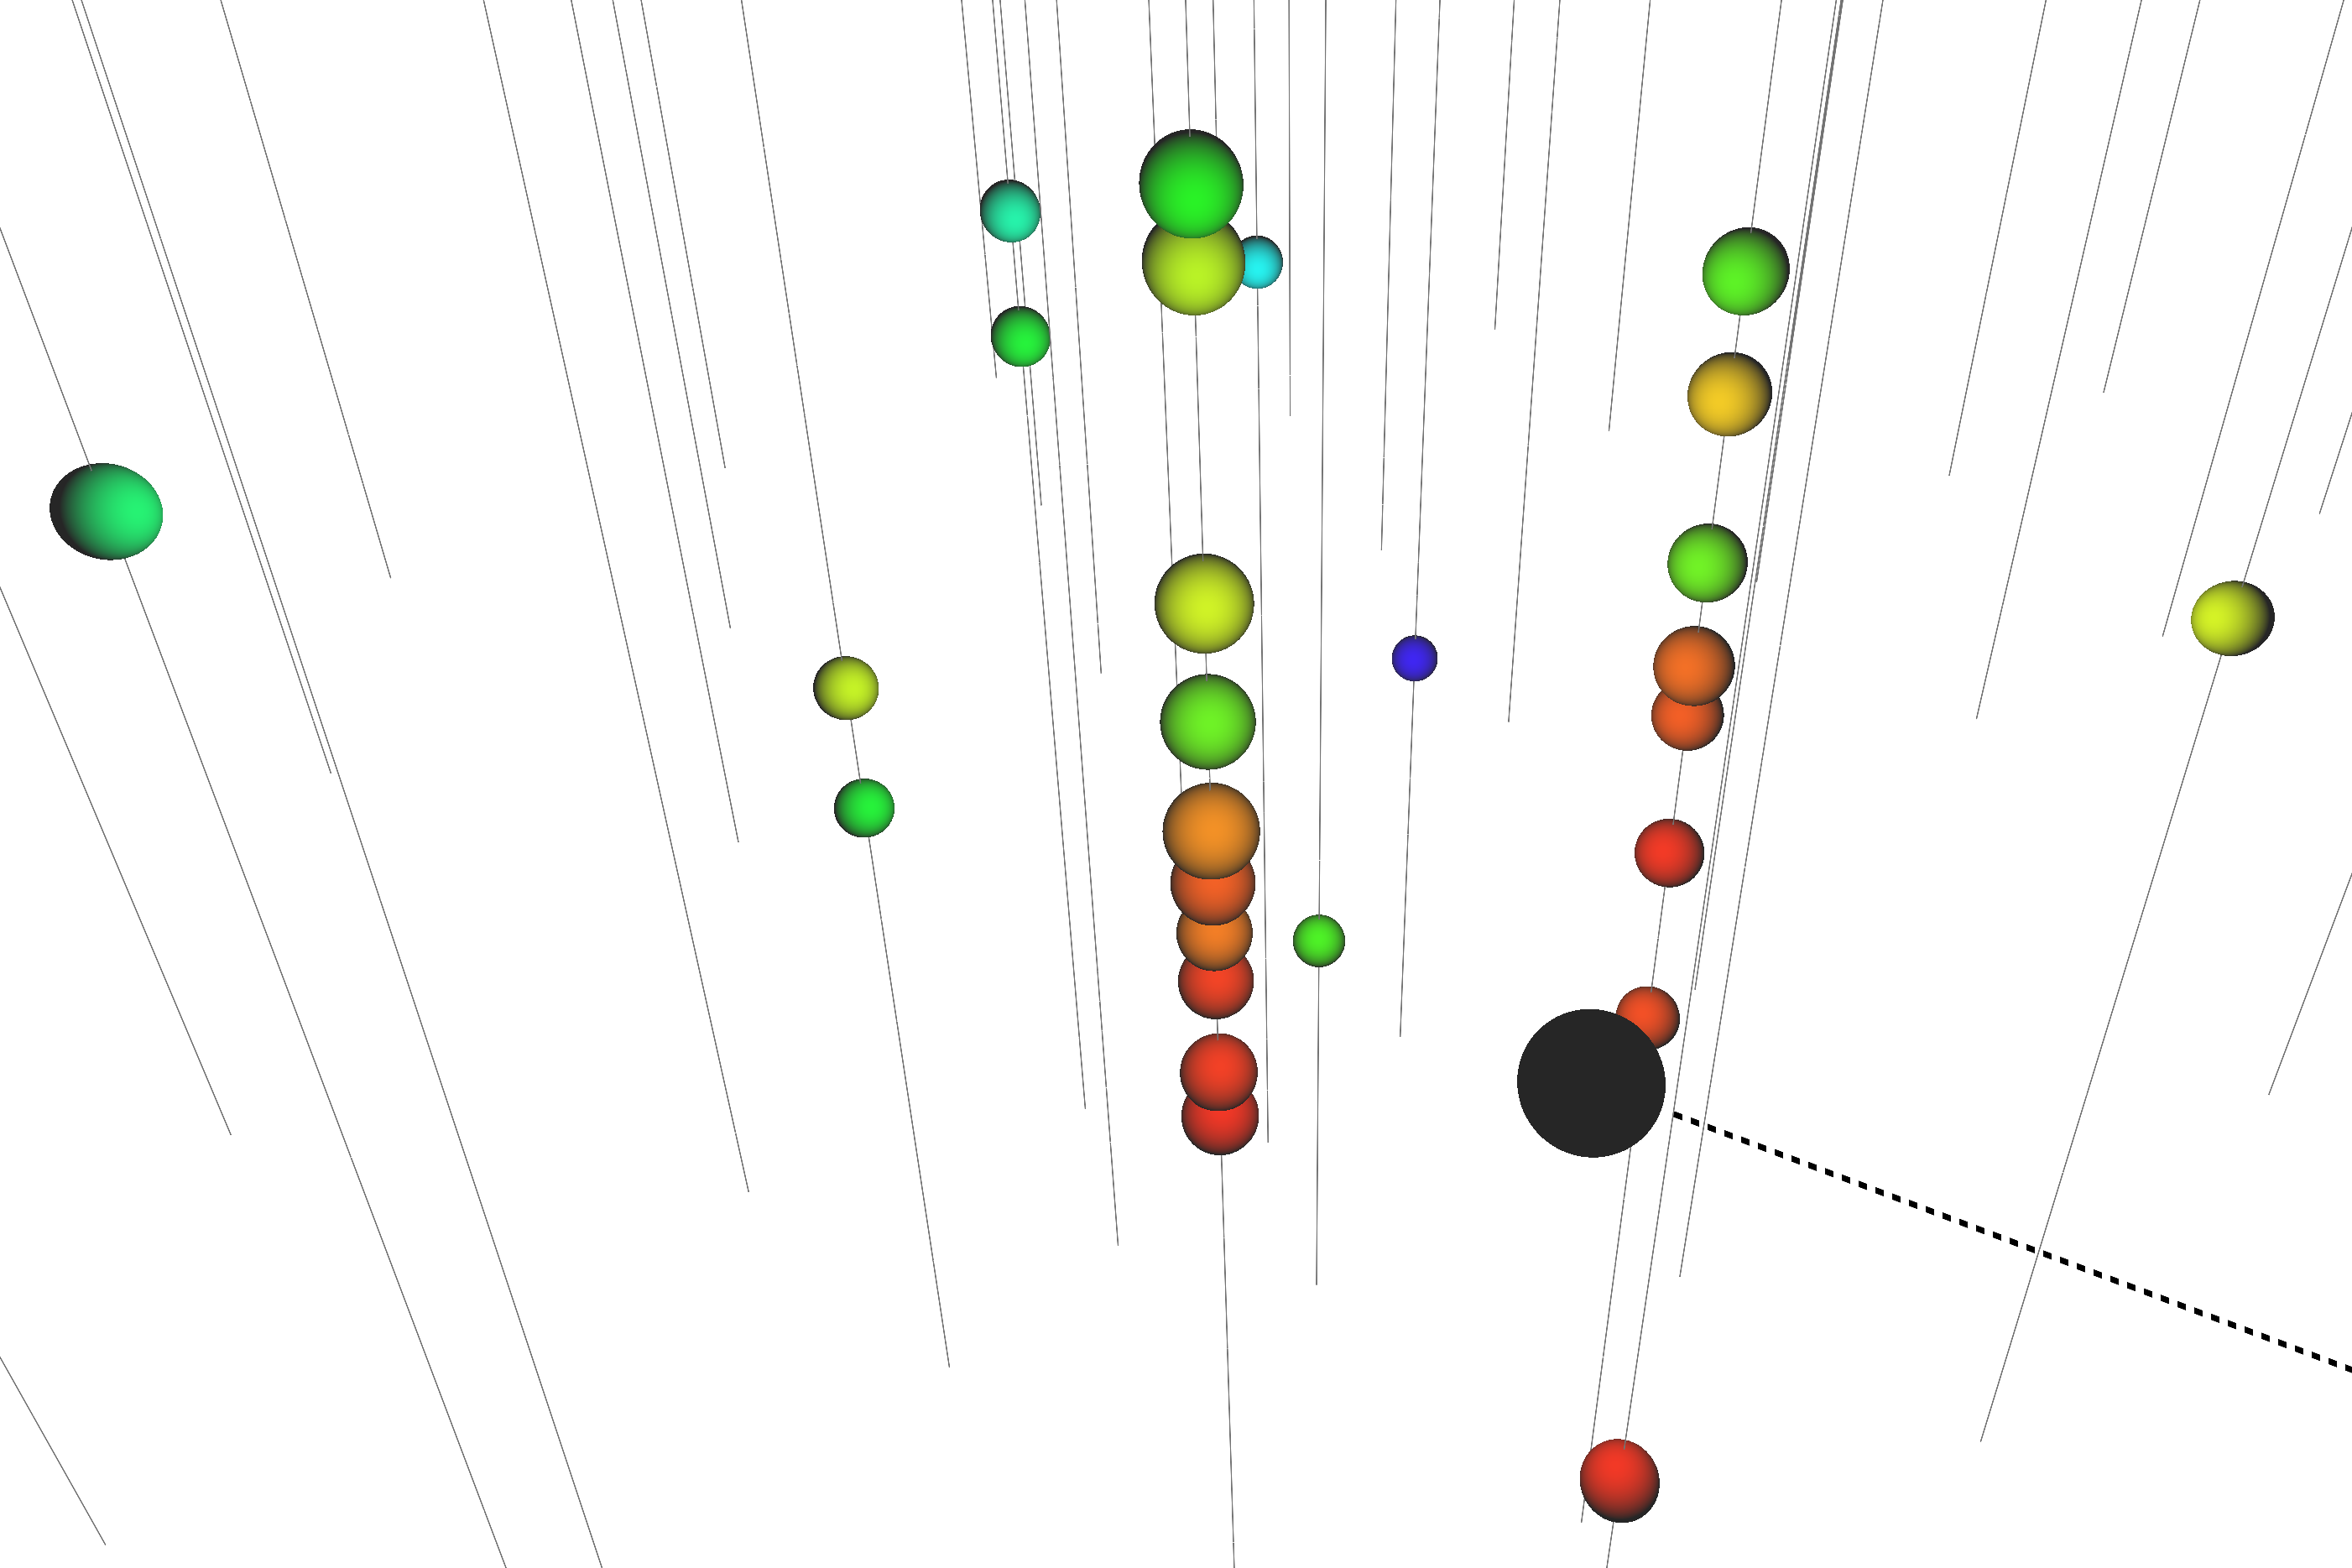
\includegraphics[width=\textwidth]{figures/icecube/eventviews/NuECC_with_neutrino_2_crop.png}
%     \caption{A simulated low energy $\nu_e$-CC neutrino interaction with an energy of 25 GeV inside the DeepCore sub-volume. The true neutrino direction is shown as the black dashed line, and the vertex as the black, round marker.}
%     \label{fig:emcasc-view}
% \end{marginfigure}
% \subsection{Tracks}
For muon-neutrinos, a muon is produced in the CC interaction which can then travel a significant distance through the ice beyond the extent of the initial hadronic shower, creating a track-like signature that sticks out of the cascade.
An idealized version of such an event is shown in the right panel of figure~\ref{fig:idealized_signatures}.

%The signal that such an interaction at an energy of 25~GeV produces in the DeepCore volume is shown in figure~\ref{fig:lowen-track-view}.
% \begin{marginfigure}
%     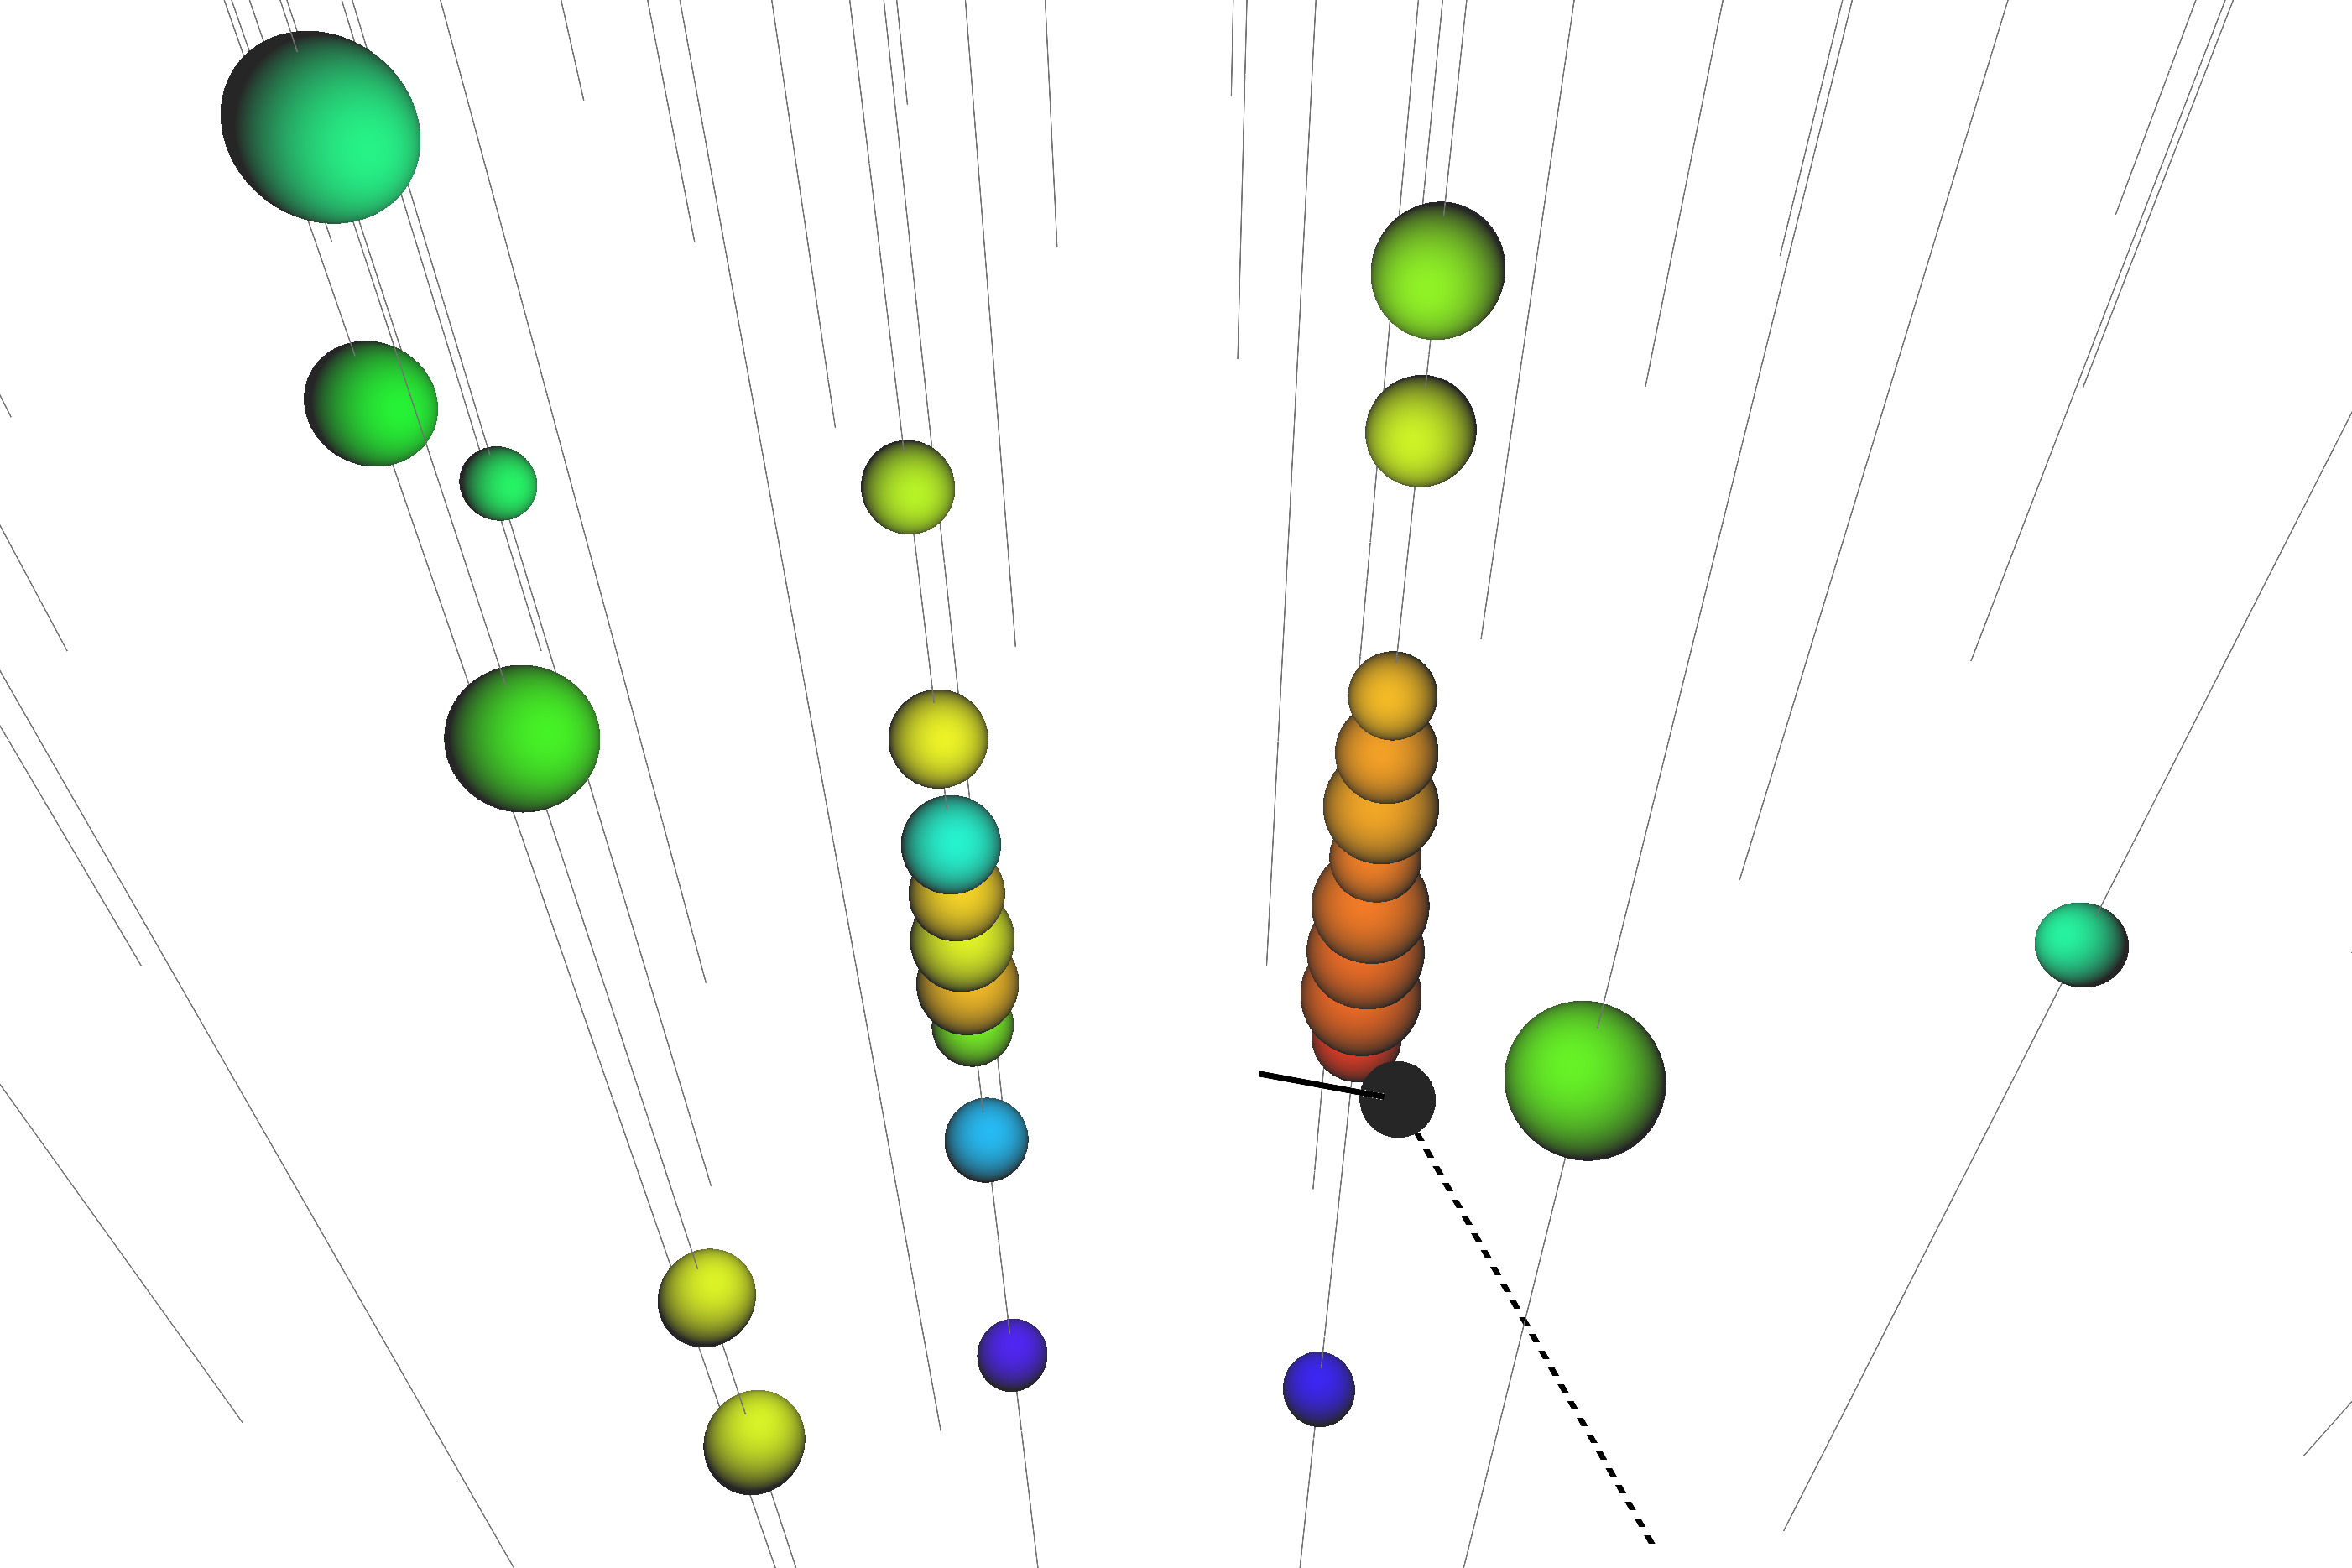
\includegraphics[width=\textwidth]{figures/icecube/eventviews/NuMuCC_with_neutrino_2_shorter_cmap_range_crop.png}
%     \caption{A simulated low energy \numucc neutrino interaction with an energy of 25~GeV inside the DeepCore sub-volume, with an outgoing 8 GeV $\mu^-$ indicated with the black, solid line (track).}
%     \label{fig:lowen-track-view}
% \end{marginfigure}
Charged-current interactions of tau-neutrinos produce a tauon that decays after a short distance, creating a second EM or hadronic shower at the point of its decay.
At TeV-scale energies, the distance covered by the tauon before its decay can be large enough to make the separation between the two showers resolvable, creating a \emph{double-bang} signature consisting of two cascades.
At energies below 100~GeV that are more relevant to this work, however, the two cascades are too close together to be cleanly separable and they are effectively approximated as a single cascade as well.
About 17\% of tauons produce a muon upon decay, creating a track-like signature as well\cite{pdg}.

A summary of the secondary particles and corresponding signatures for each type of neutrino interaction is given in \reftab{interaction-signatures}.
% \begin{marginfigure}
%     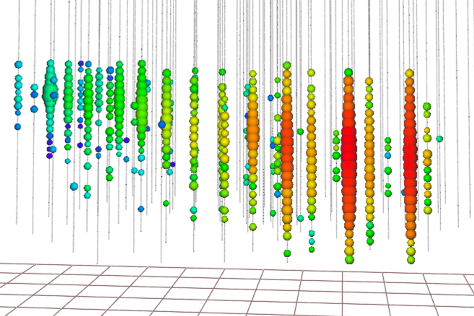
\includegraphics[width=\textwidth]{figures/icecube/eventviews/numucc_TeV_crop.png}
%     \caption{A high energy event (IceCube-170922A) with estimated energy of about 290 TeV. \cite{IceCube:2018dnn}}
%     \label{fig:txs-event}
% \end{marginfigure}

\tikzstyle{emcasc}=[shade,left color=blue!50,right color=blue!20, draw=blue]
\tikzstyle{hadcasc}=[shade,left color=red!50,right color=red!20, draw=red]
\tikzstyle{muon}=[draw=ProcessBlue, thick]
\tikzstyle{nu}=[densely dotted]
\tikzstyle{tau}=[draw=red]

\newcommand{\drawnuecc}{
    \begin{tikzpicture}
        \node (vertex) at (0, 0) {};
        \draw (-0.7, -0.1) node [anchor=south] {$\nu$} [nu] -- (vertex.center);
        \draw (vertex.center) +(0:0.3)[hadcasc,rotate=30] ellipse (0.3 and 0.15);
        \node [anchor=west,red] at (30:0.6) {hadrons};
        \draw (vertex.center) -- +(-30:0.1) +(0:0.4) [emcasc,rotate=-30] ellipse (0.3 and 0.15);
        \node [anchor=west,blue] at (-30:0.6) {$e^\pm$};
    \end{tikzpicture}
}

\newcommand{\drawnumucc}{
    \begin{tikzpicture}
        \node (vertex) at (0, 0) {};
        \draw (-0.7, -0.1) node [anchor=south] {$\nu$} [nu] -- (vertex.center);
        \draw (vertex.center) +(0:0.2)[hadcasc,rotate=30] ellipse (0.2 and 0.1);
        \node [anchor=south west,red] at (30:0.4) {hadrons};
        \draw (vertex.center)[muon] -- +(0:1.0) node [anchor=west,ProcessBlue] {$\mu^\pm$};
    \end{tikzpicture}
}

\newcommand{\drawnutaucc}{
    \begin{tikzpicture}
        \node (vertex) at (0, 0) {};
        \draw (-0.7, -0.1) node [anchor=south] {$\nu$} [nu] -- (vertex.center);
        \draw (vertex.center) +(0:0.2)[hadcasc,rotate=30] ellipse (0.2 and 0.1);
        \node [anchor=south west,red] at (30:0.4) {hadrons};
        \draw (vertex.center)[tau] -- +(-30:0.3) node (taudecay) {};
        \draw (taudecay.center) [nu] -- +(-40:0.75);
        \draw (taudecay.center) ++(10:0.3) [shade,left color=red!50,right color=blue!20, draw=gray,rotate=-10] ellipse (0.3 and 0.15) +(10:0.3) node [anchor=west,gray] {hadrons or $e^\pm$};
    \end{tikzpicture}
}

\newcommand{\drawnutauccmu}{
    \begin{tikzpicture}
        \node (vertex) at (0, 0) {};
        \draw (-0.7, -0.1) node [anchor=south] {$\nu$} [nu] -- (vertex.center);
        \draw (vertex.center) +(0:0.2)[hadcasc,rotate=30] ellipse (0.2 and 0.1);
        \node [anchor=south west,red] at (30:0.4) {hadrons};
        \draw (vertex.center)[tau] -- +(-30:0.3);
        \draw (vertex.center) ++(-30:0.3)[muon] -- +(-10:0.7) node [anchor=west,ProcessBlue] {$\mu^\pm$};
        \draw (vertex.center) ++(-30:0.3)[nu] -- +(-35:0.7);
    \end{tikzpicture}
}

\newcommand{\drawnunc}{
    \begin{tikzpicture}
        \node (vertex) at (0, 0) {};
        \draw (-1, -0.1) node [anchor=south] {$\nu$}[nu] -- (vertex.center);
        \draw (vertex.center) +(0:0.2)[hadcasc,rotate=30] ellipse (0.2 and 0.1);
        \draw (vertex.center)[nu] -- +(-10:0.6);
    \end{tikzpicture}
}

\begin{table}
    \centering
    \begin{tabular}{p{0.1 \linewidth}cc}
         interaction & secondary particles & signature \\
         \toprule
         $\nu_e$ CC &  \drawnuecc &  cascade\\
         \midrule
         $\nu_\mu$ CC &  \drawnumucc &  cascade + track\\
         \midrule
         $\nu_\tau$ CC (83\%~BR) &  \drawnutaucc &  cascade\\
         $\nu_\tau$ CC (17\%~BR) &  \drawnutauccmu &  cascade + track\\
         \midrule
         $\nu$ NC &  \drawnunc &  cascade\\
    \end{tabular}
    \caption{Secondary particles and signatures produced by each type of neutrino interaction.}
    \label{tab:interaction-signatures}
\end{table}

\subsection{Atmospheric muons}
Atmospheric muons are a significant background for oscillation measurements in DeepCore.
Not only do they make up the majority of events that pass the initial DeepCore filter, but they also produce a track-like signature in the detector that is challenging to separate from that of a charged-current muon neutrino interaction.
For this reason, most of the data filtering steps described in \refsec{offline-filter} are devoted to rejecting atmospheric muons while keeping as many muon neutrinos in the sample as possible.
At energies below 100~GeV, the dominant energy loss for muons is ionization, which creates a continuous energy loss that can pass through the entirety of the instrumented volume of IceCube.
As energies increase above 100~GeV, radiative energy losses become more relevant that create a series of stochastically distributed cascades along the muon's trajectory.
The fraction of total energy loss that is concentrated in these cascades is referred to as \emph{stochasticity}.
Atmospheric muons also often arrive in bundles originating from a single interaction of cosmic rays with the upper atmosphere.
Within such a bundle, stochastic energy losses of individual muons may average out over its trajectory, such that the bundle as a whole can be approximated as a single long track with a relatively low stochasticity.


% \subsection{Systematic uncertainties not included in the measurement}
\label{sec:other-uncertainties}

Several other potential sources of systematic uncertainties were investigated during the development of the analysis presented in this work whose impact was found to be negligible.


\subsubsection{Other oscillation parameters}
\label{sec:other-oscillation-syst}

The impact of other oscillation parameters besides $\theta_{23}$ and $\Delta m^2_{13}$ on the observed signal was assessed within the bounds set by other experiments and was found to be negligible. One exception is the CP-violating phase $\delta_{\mathrm{CP}}$, which had the potential to cause a small bias in the analysis as described in the assessment of parameter impact in \refch{measurement-three-flavor}. The analyses presented in this work only test the hypothesis under which $\delta_{\mathrm{CP}}=0$ for simplicity and to produce a result that is directly comparable to that of other experiments.

\subsubsection{Depth-dependent ice properties}
\label{sec:depth-dependent-ice-properties}

In the parametrization of the uncertainties of the detector properties described in \refsec{detector-unc}, variations of the scattering and absorption coefficients are only described by global, depth-independent scaling factors.
In principle, the error on the properties of the ice could also change as a function of depth.
For instance, one would expect that the uncertainty on the ice absorption is larger in regions with increased dust deposition, because the dust will absorb the LED light that is used to calibrate the ice model.
Of particular interest for the analysis presented in this work are variations of the ice properties at length scales of the DeepCore fiducial volume located within DeepCore.
Variations at much longer scales would be indistinguishable from uniform variations given the size of the event signatures observed below 100~GeV, while variations at much shorter scales are expected to average out.
To test how significantly such a variation would impact the final level histograms, two MC sets are produced in which the scattering and absorption coefficients vary following a sigmoid function function centered in DeepCore with an amplitude of $\pm 2\%$ in opposing directions as shown in \reffig{step-function-ice-model}.
\begin{figure}
    \centering
    \missingfigure[figwidth=0.8\linewidth]{Show step function variations, see  \href{https://drive.google.com/file/d/1TV0r1VzRbRPxlQeeCuq8DaZzeQloJZ_J/view}{presentation on lowen call}.}
    \caption{Perturbation of the scattering and absorption coefficients with respect to the nominal ice model applied in additional MC sets.}
    \label{fig:step-function-ice-model}
\end{figure}
The size of this variation corresponds approximately a $1\sigma$-allowed variation according to flasher calibration data. Then, for every bin in the final analysis histogram, a linear regression is fit to the bin counts of the nominal MC set and the two variations assuming that they correspond to $\pm 2\%$ variations of a parameter.
The resulting slopes were found to be indistinguishable from pure statistical variation and it was concluded that the impact of such a hypothetical new systematic uncertainty would be insignificant.\todo{This was only done for the high-stats sample: redo for verification sample?}

%In previous oscillation studies using track-like events in the TeV energy range \sidecite{MEOWS}, this effect was found to be non-negligible. To model depth-dependent uncertainties of the ice properties, a method was developed in which the depth-dependence of the scale factor for scattering and absorption coefficients is decomposed into Fourier-modes, and the impact of each mode on the final analysis histogram can be calculated\sidecite{snowstorm}. In the analysis presented in \cite{MEOWS}, the impact of high-frequency Fourier modes was found to be negligible and therefore the uncertainties of the bulk ice was modeled using the lowest fourth modes.

\subsubsection{Atmospheric density}
\todo[inline]{Describe test of atmospheric density impact (or get feedback if that is even necessary}

\subsubsection{$K/\pi$-air interactions}
\todo[inline]{Describe this part, although it might also be just too much.}

% \section{Data Processing}
\label{sec:data-processing}

\subsection{Trigger}
As described in section \ref{sec:dom-daq}, the high-frequency ATWD waveform digitization in each DOM is triggered when it and its adjacent or next-to-adjacent neighbors on the same string record a voltages of at least 0.25 PE-equivalent within a $\pm$1~$\mu$s time window, which is referred to as the Hard Local Coincidence (HLC) condition. Data acquisition for DeepCore is triggered when this condition is fulfilled for at least three DOMs inside the DeepCore fiducial volume within a $\pm$2.5~$\mu$s window. If this condition is met, the waveforms for all DOMs that have observed voltages of at least 0.25~PE within a $\pm$10~$\mu$s time window centered around the trigger time are recorded. A DOM that is included in this readout but for which the HLC condition has not been met is said to fulfill the \emph{Soft Local Coincidence} (SLC) condition. The DeepCore trigger rate is less than 10~Hz and will trigger on \~70\% of $\nu_\mu$ events at 10~GeV and >90\% of $\nu_\mu$ events at 100~GeV\cite{DeepCore}.

\subsection{Online Filter}

Once the trigger condition is met, the recorded waveforms within the trigger window are converted into reconstructed pulses and are then passed into a set of \emph{online} filters (i.e. filters running on hardware at the Pole). These filters are each designed to select events that are relevant to different physics measurements that are performed within the IceCube collaboration. For the purposes of the analysis presented in this thesis, events are selected using the \emph{DeepCore filter}. This filter is designed to select events that start inside the DeepCore fiducial volume and to reject those that are consistent with muons entering the detector from the outside.
\begin{marginfigure}
    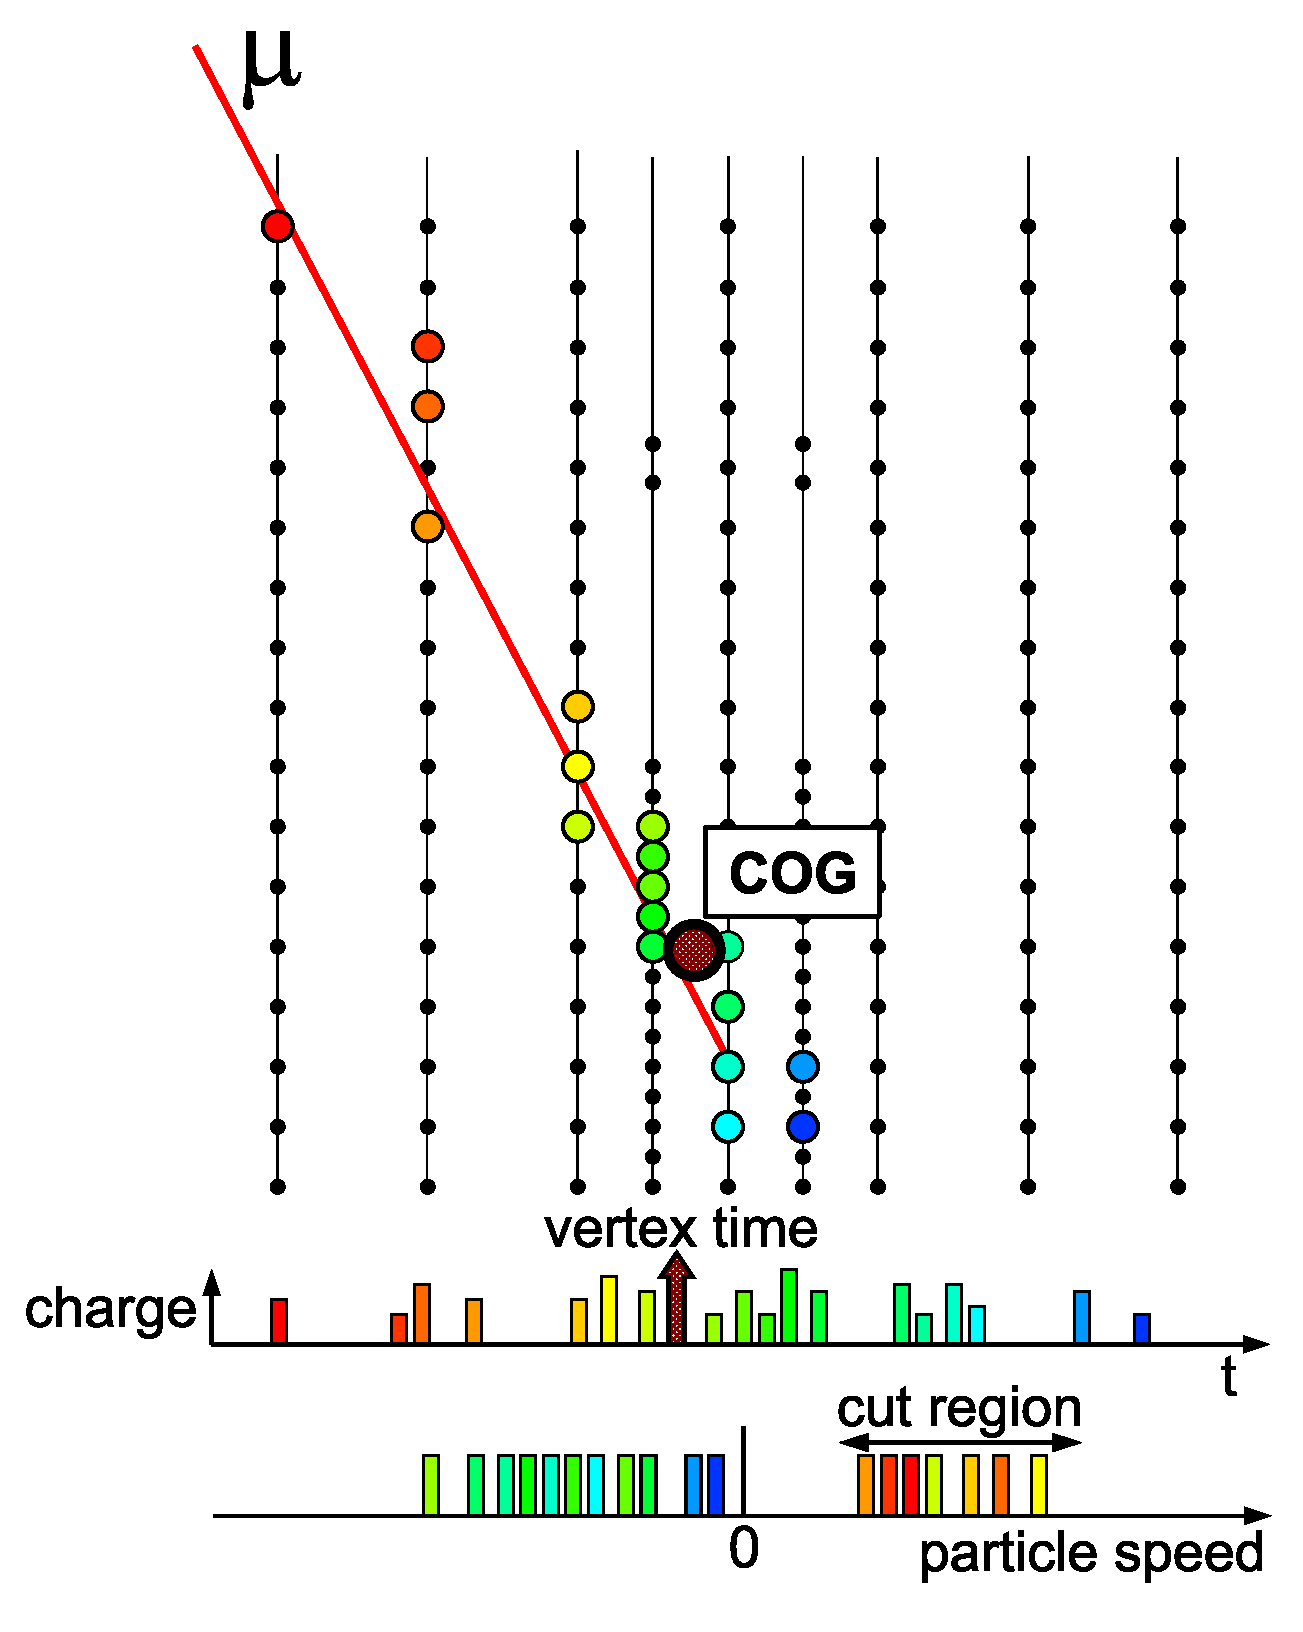
\includegraphics[width=\textwidth]{figures/icecube/eventviews/FilterDiagram.pdf}
    \caption{Example of an event that would be rejected by the online filter algorithm. DOMs that have observed light are highlighted in color depending on time from red (early hits) to blue (late hits). DOMs that have not observed any light are shown as black dots. Figure taken from \cite{DeepCore}.}
    \label{fig:online-filter-event}
\end{marginfigure}
The filter first applies a noise cleaning algorithm based on a coincidence condition between hits on different DOMs, where hits in DOMs for which the HLC condition was met are always kept. The cleaned hit series is split between those hits that fall within the DeepCore fiducial volume and those outside of it. The veto algorithm then calculates the COG in space and time of the hits inside the fiducial volume and then the velocity that a signal would have to travel from each hit occurring outside the fiducial volume to coincide with the COG. If this velocity is close to the speed of light (between $0.25\;\mathrm{ns/s}$ and $0.4\;\mathrm{ns/s}$) for at least one hit, the event is rejected because it is consistent with a muon traveling through the veto region and entering DeepCore. Figure~\ref{fig:online-filter-event} shows an example of an event that would be rejected by the online filter. Only events passing the trigger and filter condition are sent North via satellite for further \emph{offline} filtering.

\subsection{Offline Filter}

The offline filter is separated into subsequently applied \emph{levels}, referred to as L3, L4, and L5, where each level reduces the amount of background (atmospheric muons and noise) by approximately an order of magnitude while keeping most of the DeepCore starting events that are the target of the selection.

\subsubsection{Level 3}
At the lowest offline filter level, L3, cuts are applied to simple variables that remove the most easily identifiable background events while using only few computational resources. The variables aimed at cutting noise consist mostly of different DOM hit counts within hit series to which noise cleaning algorithms have been applied. The cuts aimed at removing muons consist of conditions on the number of hits in the veto region as well as conditions on the vertical position of the first HLC hit. The distribution for one of the variables used in the L3 filter is shown in figure~\ref{fig:l3-var-cleaned-full-time-length}. It is apparent from the distributions that there is a significant population of events in data with large values of the plotted variable that does not exist in simulation. These events are discarded, improving the agreement between data and simulation for events passing the L3 filter.
\begin{figure}
    \centering
    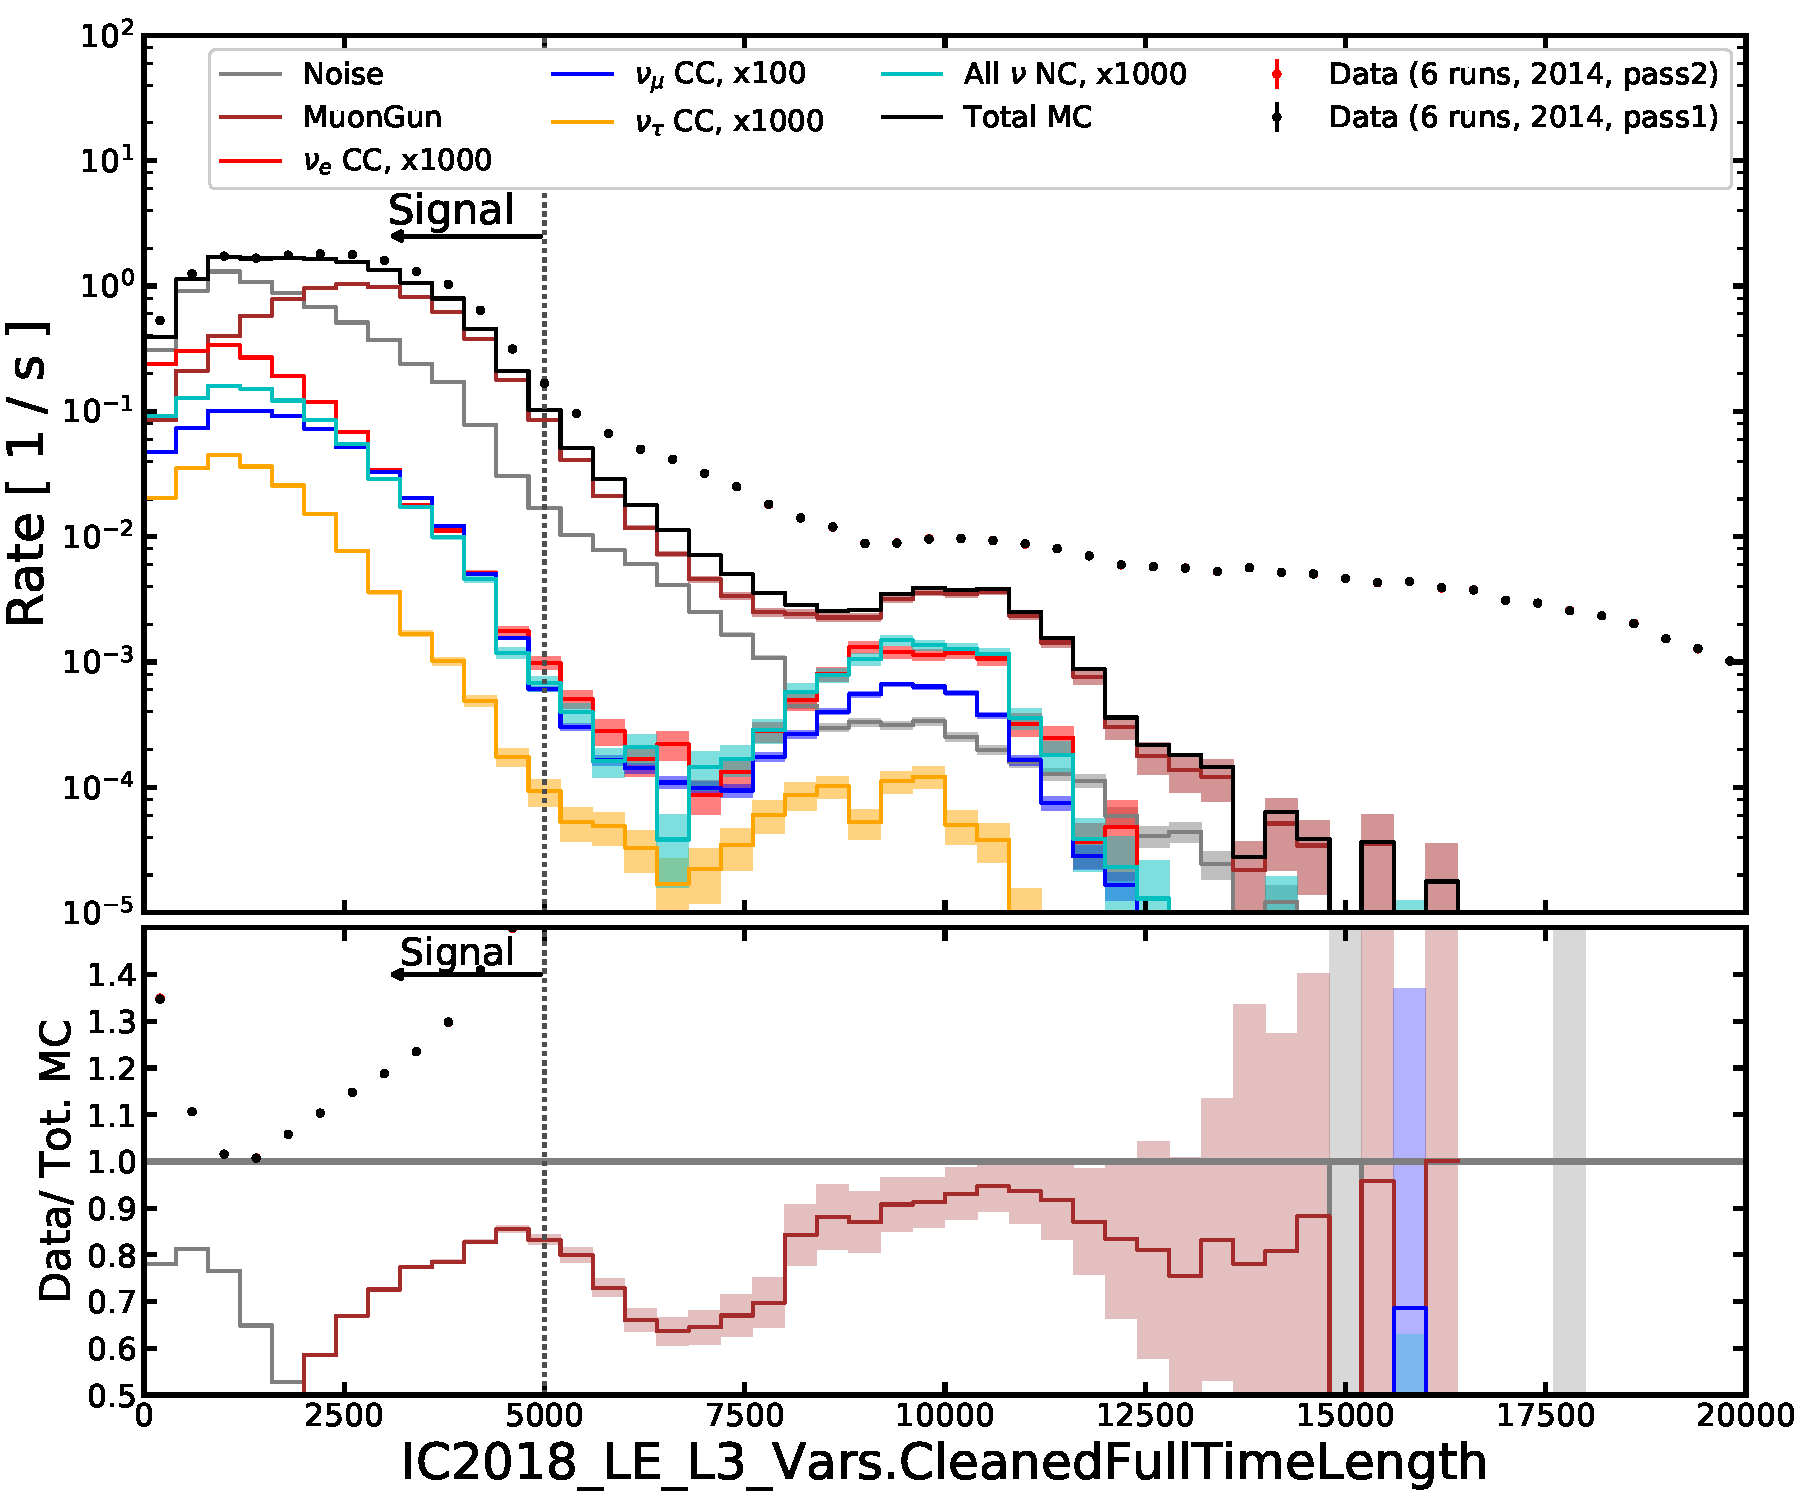
\includegraphics[width=7 cm]{figures/icecube/selection/IC2018_LE_L3_Vars_CleanedFullTimeLength.pdf}
    \caption{Distribution of one of the variables used in the L3 offline filter, the time between the last hit and the first hit after noise cleaning. Histograms show the distributions in simulated data separated by particle and interaction type, data points with error bars show the distribution of real data. The bottom panel shows the ratio between data and simulation. Events falling on the "signal" side of the histogram are passed to the next filter level.}
    \label{fig:l3-var-cleaned-full-time-length}
\end{figure}

\subsubsection{Level 4}
In the next level, L4, more advanced selections based on the output of Boosted Decision Trees (BDTs) are applied, with a separately trained BDT for noise and muon rejection, respectively. The output of each BDT is a probability score between zero (background-like) and one (signal-like).  The inputs into the BDT aimed at noise rejection consist of hit counts in cleaned hit series and variables that characterize the geometric and temporal spread of the observed hits, such as the full width half maximum (FWHM) of the hit times. The BDT is trained using simulated pure noise and neutrino events. Events are passing the L4 noise cut if the BDT score is above 0.7, which reduces the number of pure noise events by two orders of magnitude from 36.6~mHz to approximately 0.3~mHz. The BDT that is used to reject atmospheric muons also takes simple variables as its input that consist mostly of different veto hit counts and variables that characterize the distribution of z-coordinates of the observed hits as well as their radial distance with respect to the center of the DeepCore fiducial volume. In contrast to the noise BDT, however, the muon BDT is trained using real data and simulated neutrino events, with the goal of rejecting data events. This is possible because the data sample consists to 99\% of atmospheric muons at this stage of the event selection. Events are passing the L4 muon cut if the output score from the muon BDT is above 0.65, removing 94\% of all muon events while keeping 87\% of all neutrinos. The distributions of the output scores of both BDTs are shown in figure~\ref{fig:l4-bdt-output}.
\begin{figure*}
    \centering
    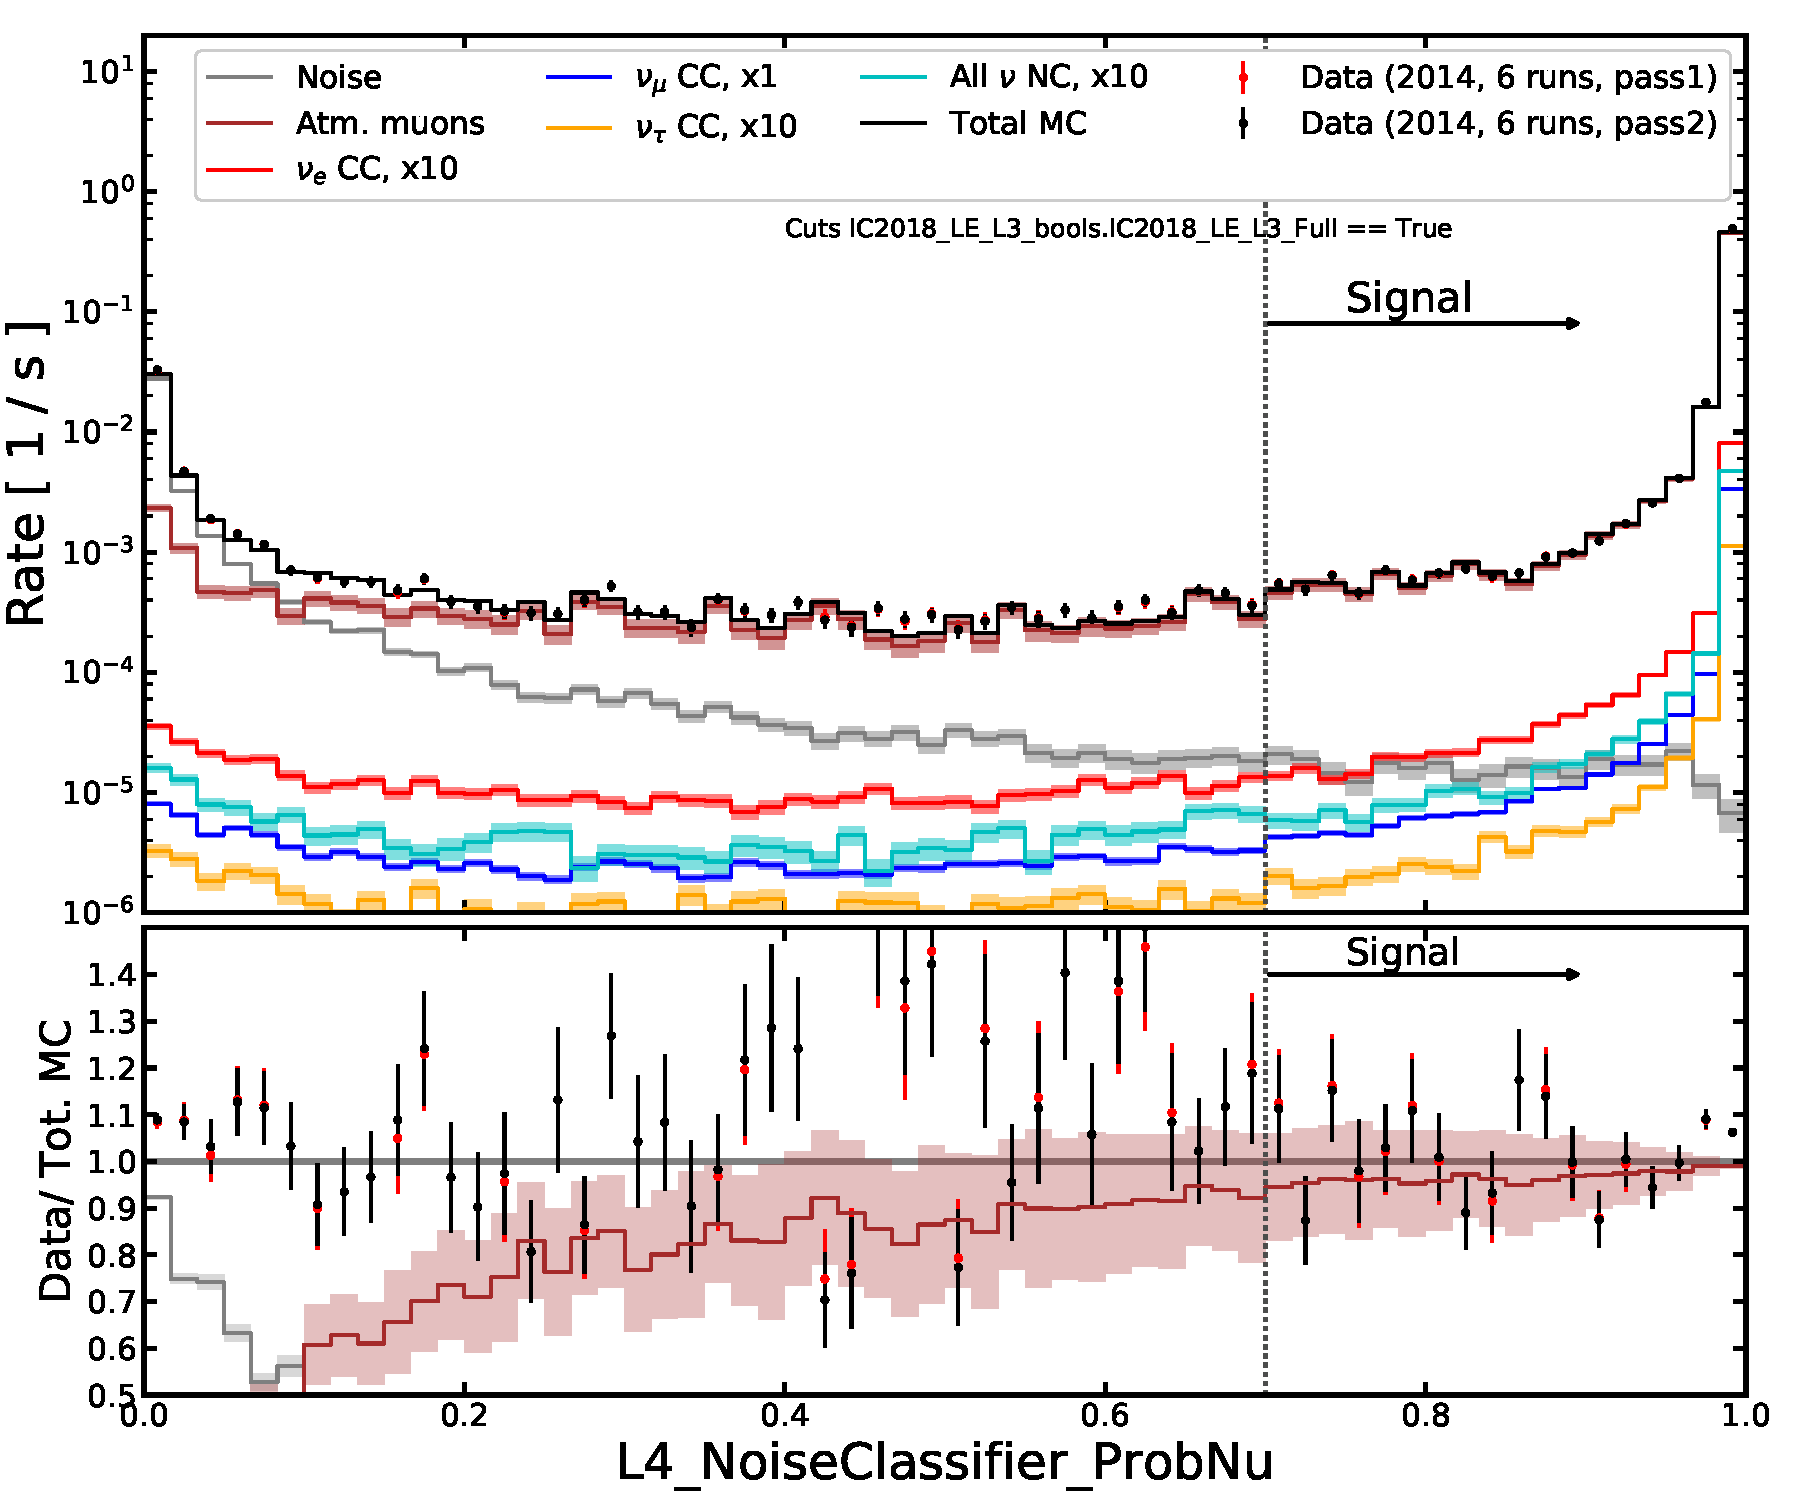
\includegraphics[width=7 cm]{figures/icecube/selection/L4_noiseBDT_L4_NoiseClassifier_ProbNu.pdf}
    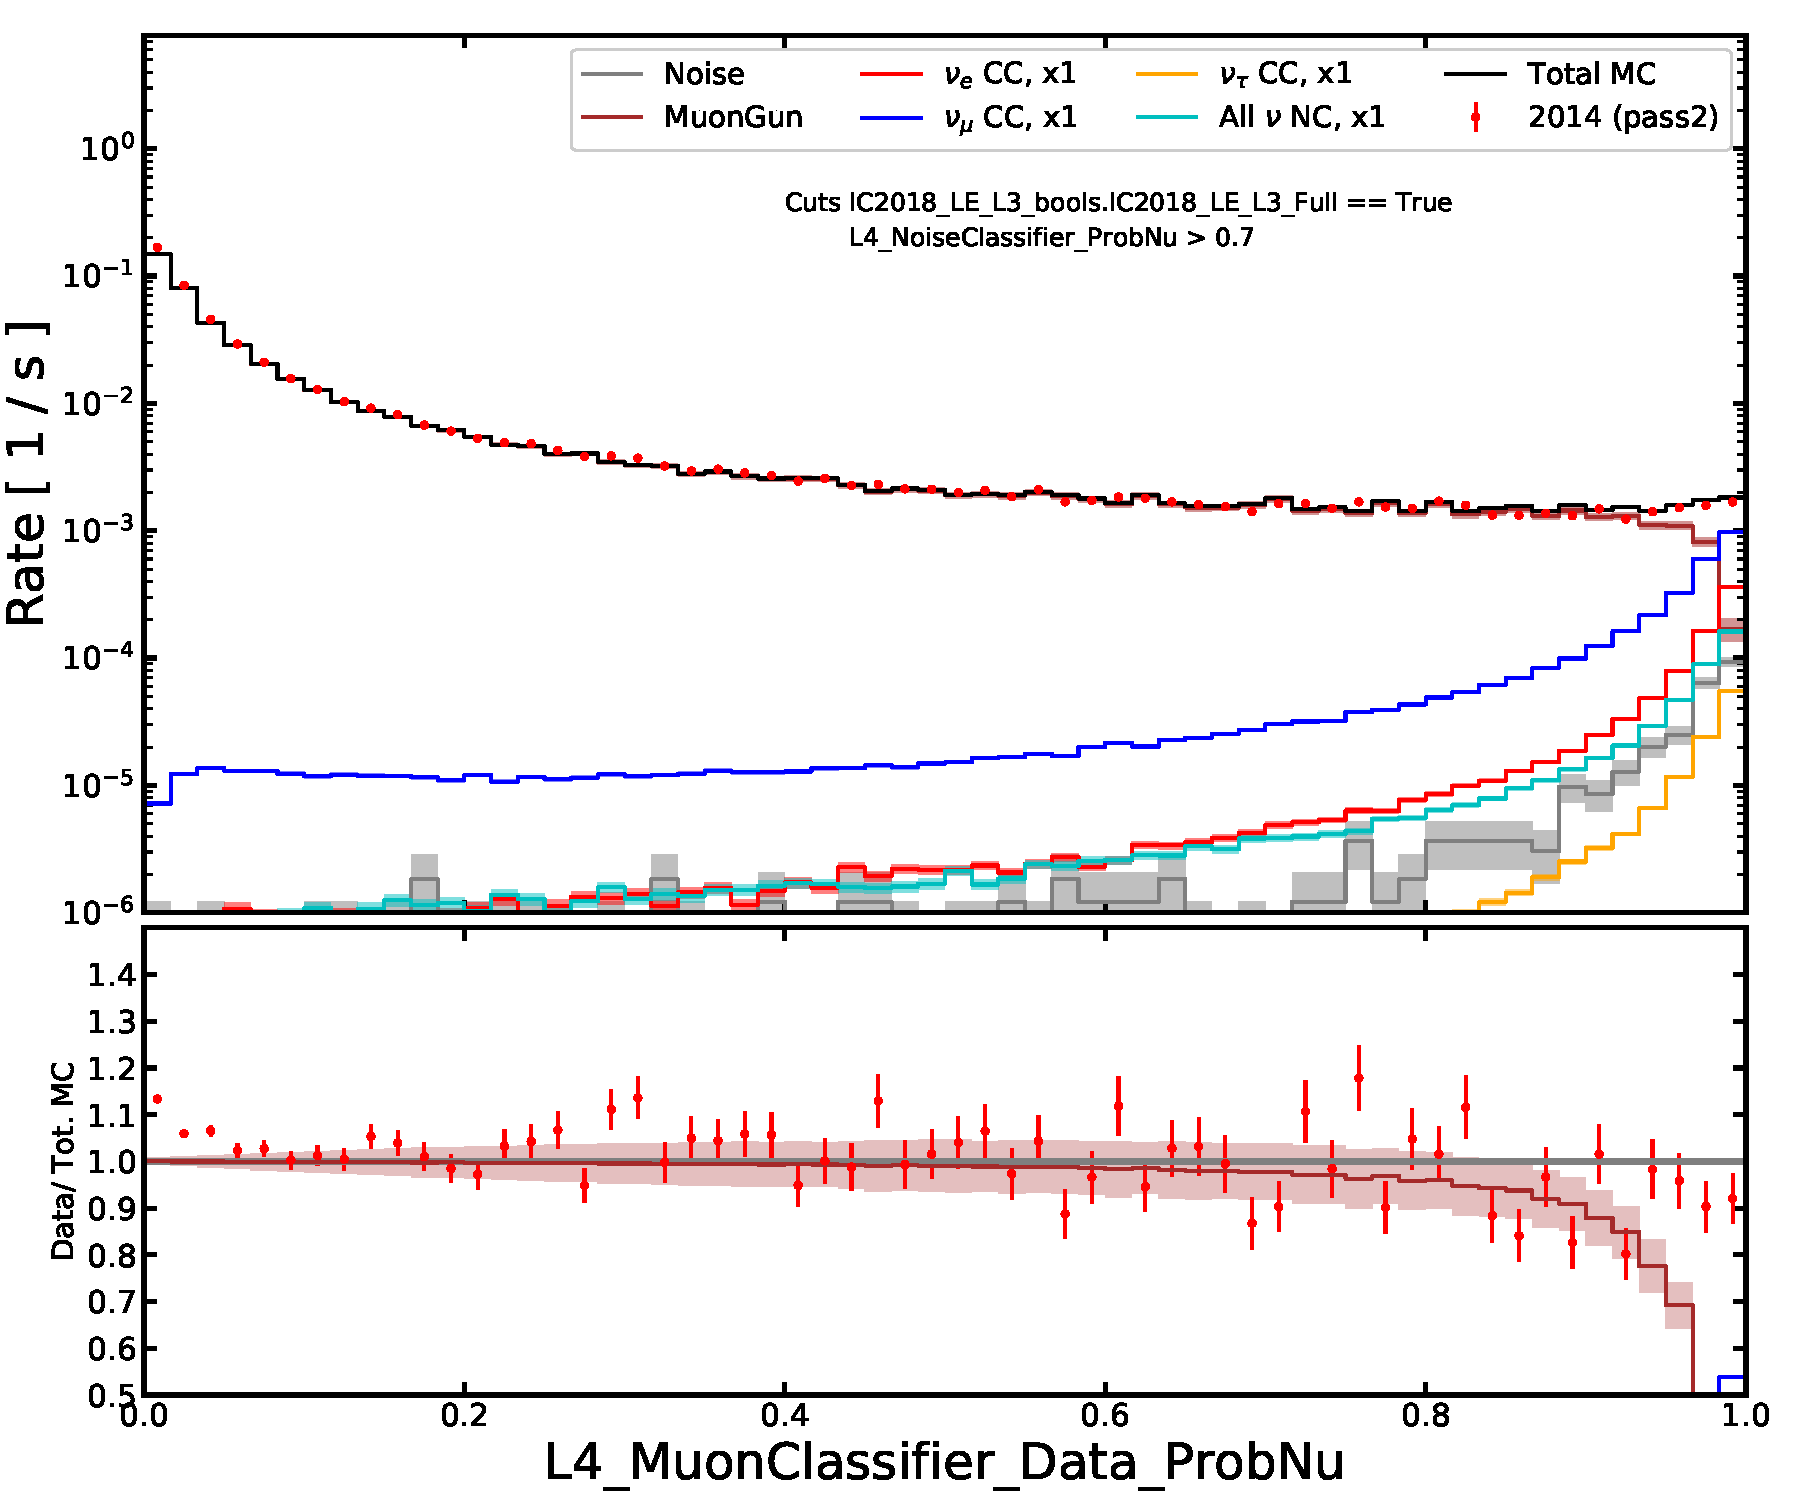
\includegraphics[width=7 cm]{figures/icecube/selection/L4_muon_L4_MuonClassifier_Data_ProbNu.pdf}
    \caption{Distribution scores for the noise (left) and muon (right) BDT. The distributions of the muon classifier are shown for events where the score of the noise BDT is greater than 0.7.}
    \label{fig:l4-bdt-output}
\end{figure*}

\subsubsection{Level 5}
The final offline filter level that is applied before the event reconstruction step is L5. This filter searches specifically for hits occurring in un-instrumented \emph{corridors} within the IceCube array through which an atmospheric muon can sneak into the DeepCore volume while evading previous veto cuts. In addition, events with more than seven hits in the outermost strings of the IceCube array or that have a down-going pattern of hits in the uppermost region of the detector are vetoed to remove events containing atmospheric muons entering the detector coincidentally with neutrinos. The distribution for one of the corridor variables and one of the muon rejection variables are shown in figure~\ref{fig:l5-vars}. Table~\ref{tab:l5_summary} shows the rates of each event type expected at each level of the selection up to L5 together with the efficiency of the filter at the final level.
\begin{figure*}
    \centering
    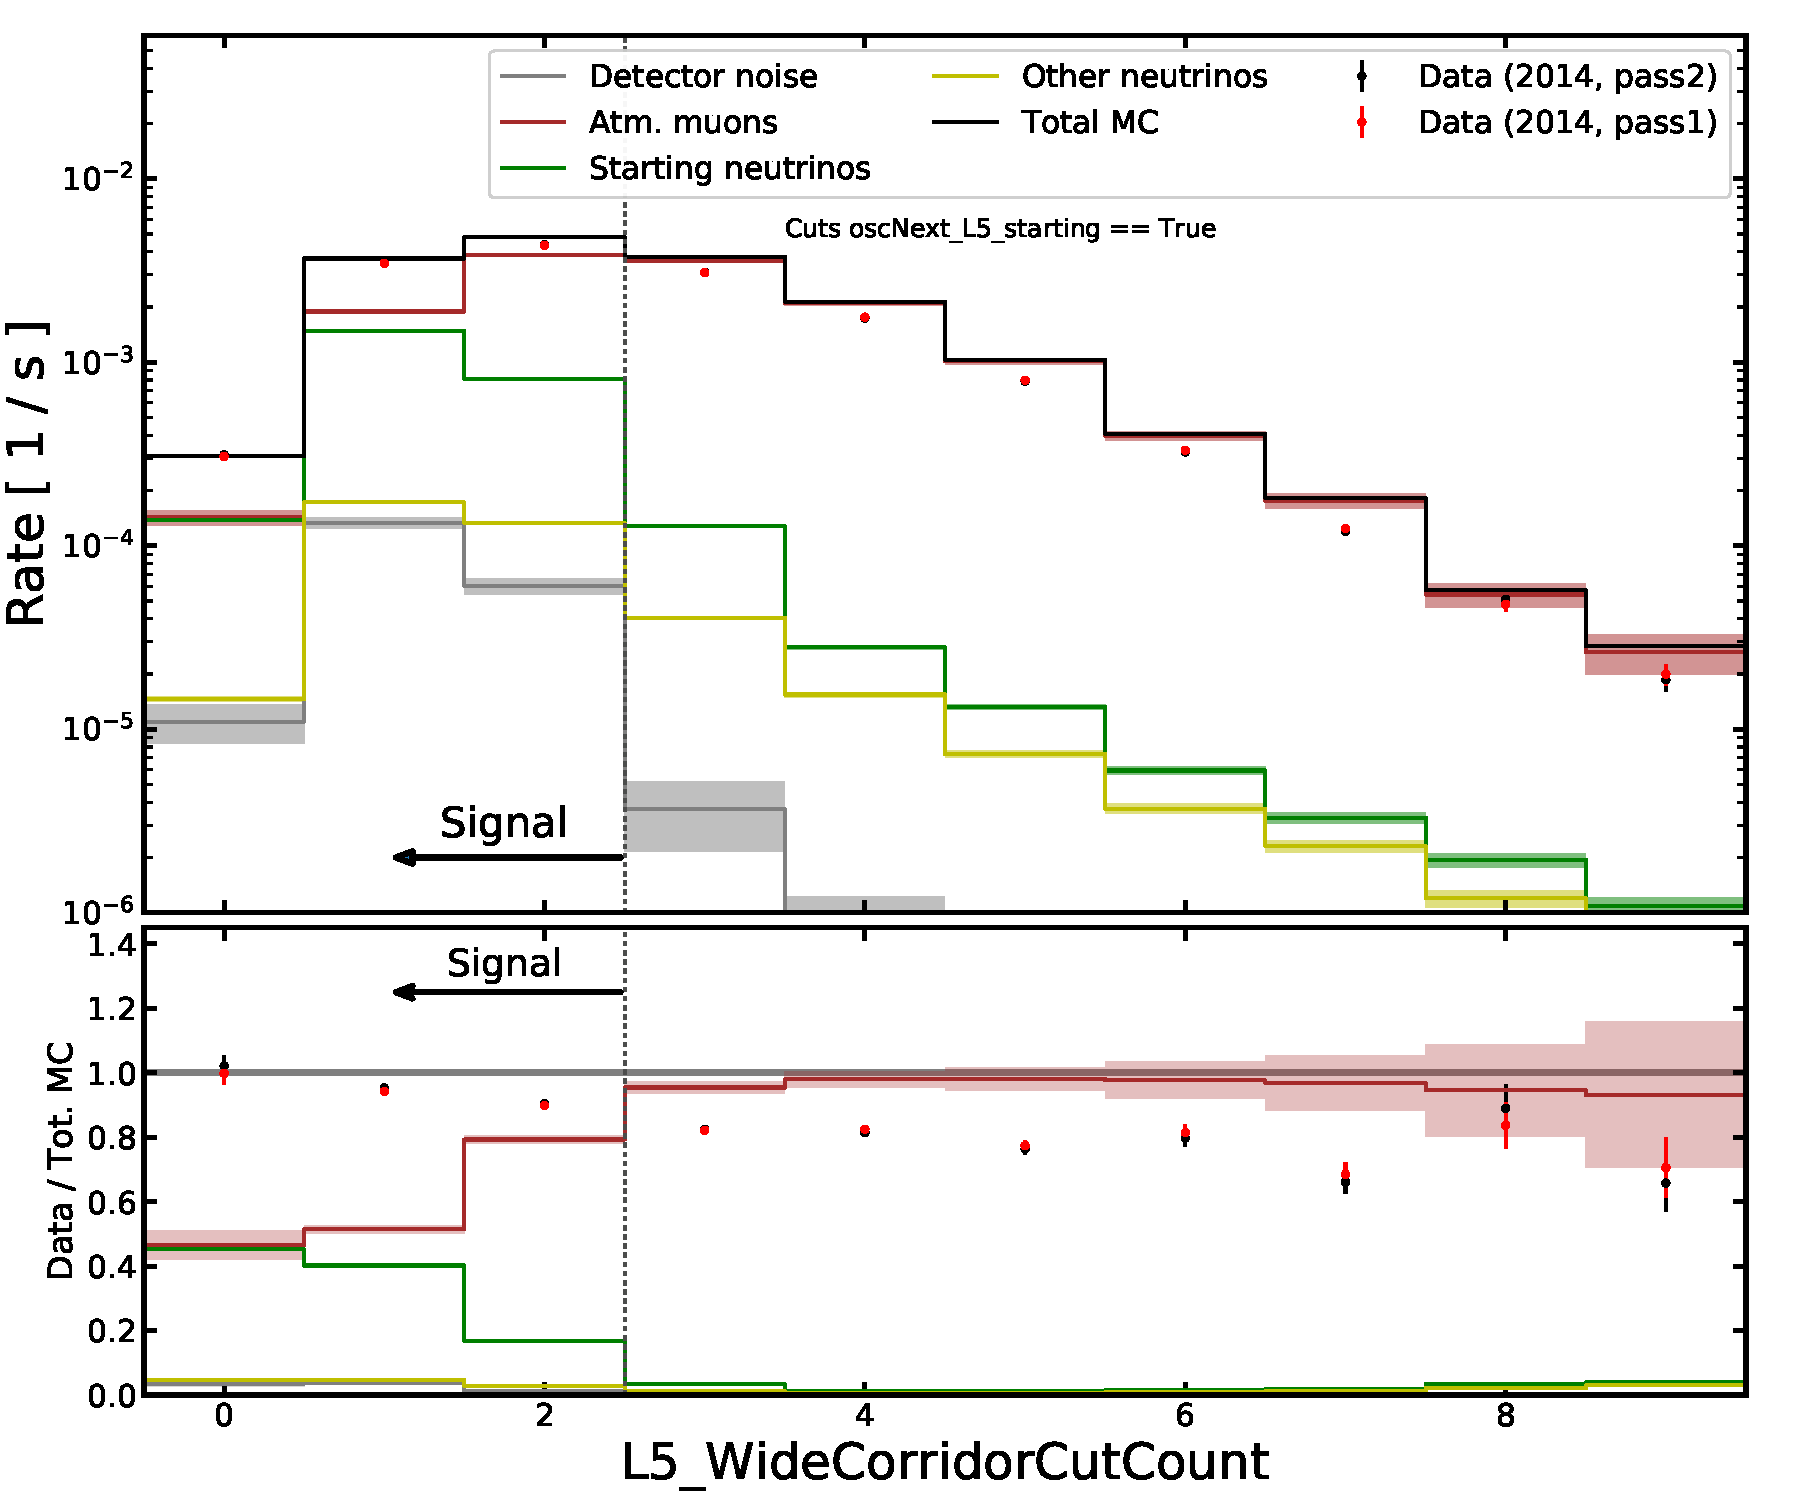
\includegraphics[width=7 cm]{figures/icecube/selection/L5_contained_L5_WideCorridorCutCount.pdf}
    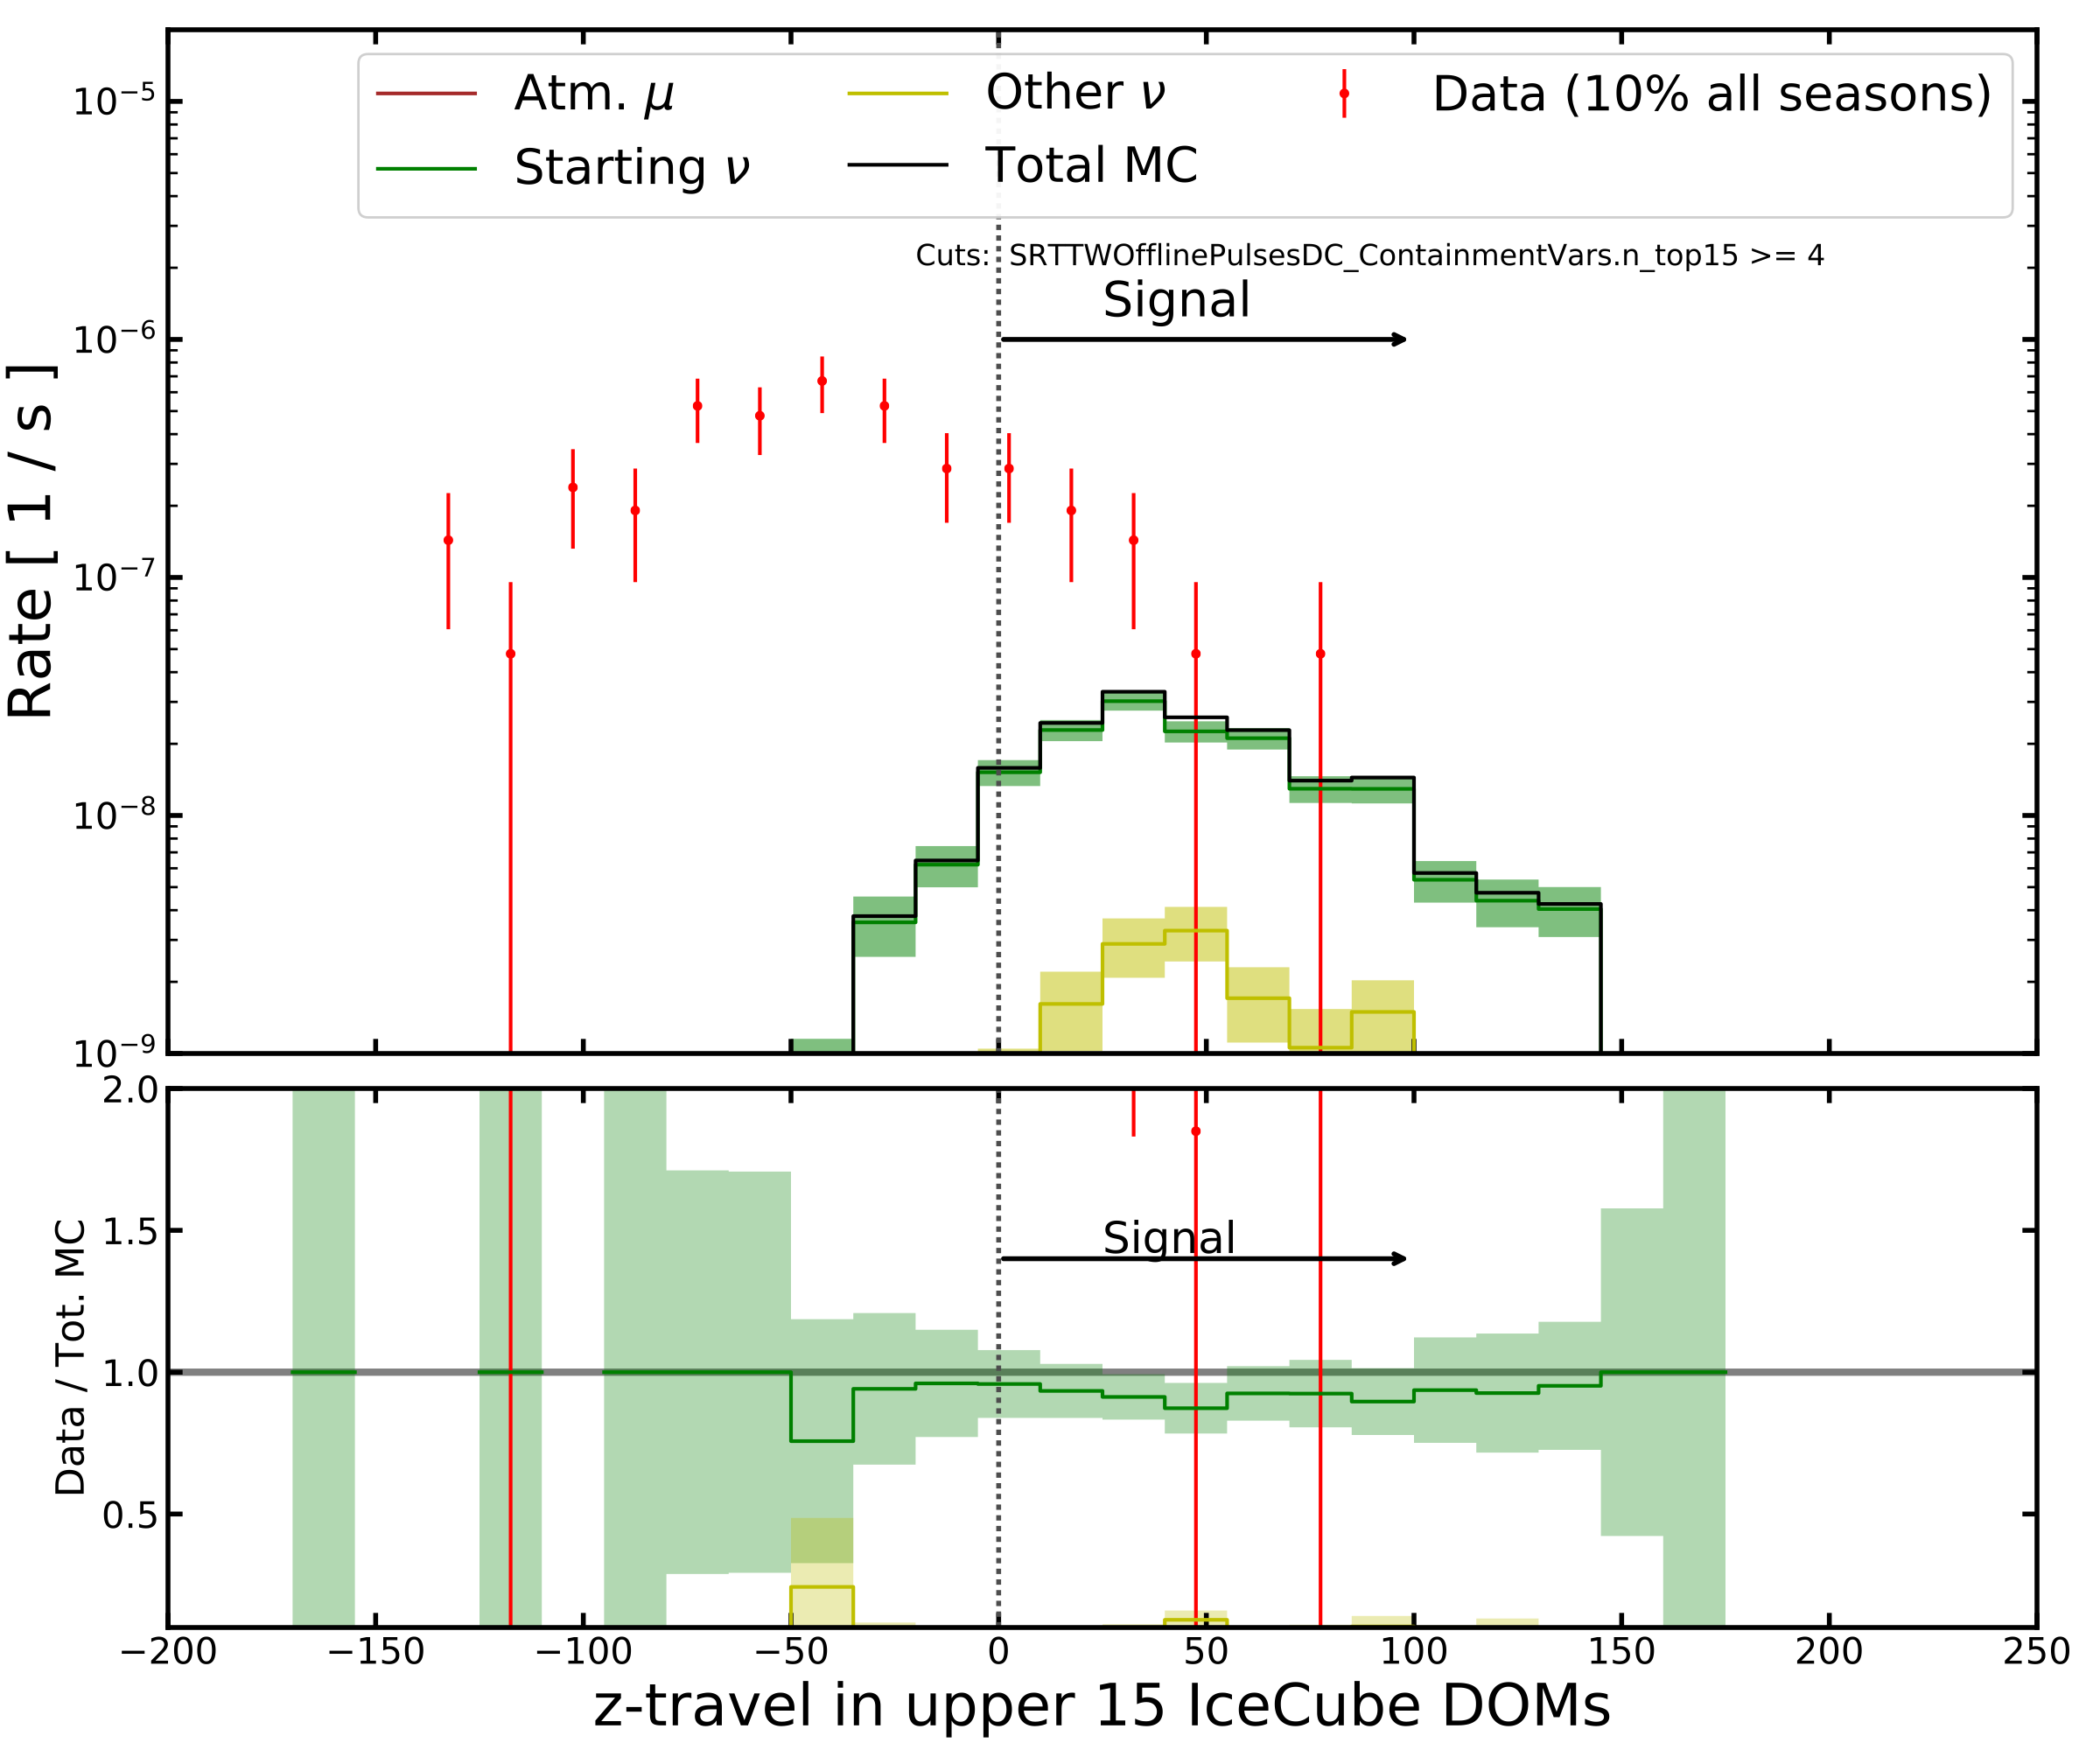
\includegraphics[width=7 cm]{figures/icecube/selection/SRTTWOfflinePulsesDC_ContainmentVars.z_travel_top15.png}
    \caption{Distributions for one of the L5 corridor cut variables (left) and one of the variables used to reject coincident muon events (right). The distribution in the right panel is shown only for events which have at least four hits in the uppermost 15 DOMs combined over all IceCube strings.}
    \label{fig:l5-vars}
\end{figure*}

\begin{table}
\begin{tabular}{lrrrrr}
Event type  & DC filter   & L3   & L4   & L5   & Eff. (\%) \\
\toprule
Atm. $\mu$         & 7273 & 505  & 28.1 & 0.93 & 0.012          \\
Pure noise         & 6621 & 36.6 & 0.28 & 0.07 & 0.001          \\
Atm. $\nu_e$ CC    & 1.61 & 0.95 & 0.84 & 0.48 & 29.8           \\
Atm. $\nu_\mu$ CC  & 6.16 & 3.77 & 3.11 & 1.39 & 22.5           \\
Atm. $\nu_\tau$ CC & 0.19 & 0.13 & 0.12 & 0.07 & 36.8           \\
Atm. $\nu$ NC      & 0.86 & 0.53 & 0.46 & 0.23 & 26.7  \\
\end{tabular}
\caption{Summary of the rates (in mHz) obtained after each level of selection. Neutrinos are weighted to an atmospheric spectrum with oscillations included.}
\label{tab:l5_summary}
\end{table}

\subsection{Event Reconstruction}
\label{sec:event-reconstruction}

After the L5 selection, the rate of muons is reduced enough such that the majority of the total sample is expected to consist of atmospheric neutrinos, and it is at this point that the event reconstruction and signature classification is run. For the measurement presented in this thesis, three reconstructed quantities are required: The zenith angle, the energy, and a proxy score that determines the flavor of a neutrino. As described in section \ref{sec:particle-signatures}, all neutrino events in DeepCore can be effectively approximated as either a cascade ($\nu_e$ CC events, all NC events, and 83\% of $\nu_\tau$ CC events) or a combination of a cascade at the neutrino interaction point with an out-going muon track ($\nu_\mu$ CC events and 17\% of $\nu_\tau$ CC events). The zenith angle can be most accurately reconstructed for track-like events due to their elongated, highly directional signature. For cascades, the reconstruction of the direction is more difficult because of their most compact and diffuse light distribution. The energy of a neutrino event is reconstructed by comparing the expected light output of a combined track and cascade hypothesis to the observed hits. Finally, the flavor proxy is calculated using variables that characterize the elongation of the observed hit signature  and the goodness-of-fit of a combined track and cascade hypothesis compared to that of a cascade-only hypothesis. The resulting score allows the separation of muon neutrino interactions from other interactions, which is ideally suitable to observe the muon neutrino disappearance oscillation channel.

\subsubsection{Zenith angle reconstruction}
The zenith is reconstructed using an old but refurbished algorithm that first removes hits from light that is likely to have undergone a significant amount of scattering and then runs a modified $\chi^2$ fit on the observation times of the remaining hits assuming that they all lie on a Cherenkov cone that would be produced by a minimally ionizing muon. Because of the required hit cleaning step, not all events present at L5 can be reconstructed in this way. However, those events that pass the cleaning condition are the cleanest, most track-like events of the entire sample and therefore can be seen as a high-quality "golden sample".



\setchapterpreamble[u]{\margintoc}
\setchapterstyle{kao}
\chapter{Simulation and Data Processing}
\labch{data-sample}


\section{Event Simulation}
\label{sec:event-simulation}
The method by which all of the measurements presented in this thesis are performed is that of \emph{Monte-Carlo (MC) forward folding}.
In a nutshell, this method involves producing a large set of simulated signal and background events that are then re-weighted in such a way that their distribution matches that of the observed data events as closely as possible.
To give reliable results, an accurate simulation of all particle interactions described in Section~\ref{sec:particle-interactions} as well as the detector electronics described in section~\ref{sec:dom-daq} is required.
The simulated and observed events are then passed through the same data processing chain described in section~\ref{sec:data-processing}.
The resulting MC simulated dataset and the observed dataset are then histogrammed in the same binning, and the weights of the MC events are adjusted to give the best match between the histograms according to a loss function as defined in section~\ref{sec:test-statistic}.

The simulation chain for neutrinos and atmospheric muons can generally be divided into three steps that are described in this chapter:
\begin{enumerate}
    \item Simulation of particle interactions
    \item Photon propagation in ice
    \item Response of detector DAQ systems
\end{enumerate}
A special case is the simulation of detector noise, for which no particle production or photon propagation is necessary.

% \subsection{Particle Interactions}

% The first step for the simulation of neutrinos and muons is to sample parameters for the primary particle, and to simulate the secondary charged particles that are produced when it interacts inside the detector. The charged components of the secondary particles are then passed on to the photon propagation step described in section~\ref{sec:photon-propagation}.

\subsection{Neutrino Interactions}

Because of the inherently low interaction rate of neutrinos, it would be impractical to simulate a constant flux of neutrinos from any particular direction, the vast majority of which would simply pass through the detector without producing any signal at all.
Instead, every simulated neutrino is forced to interact within a given volume, and the event is given a weight corresponding to the inverse of the simulated fluence,
\begin{equation}
    w = \frac{1}{F_{\mathrm{sim}}} \frac{1}{N_{\mathrm{sim}}}\;.
\end{equation}
Here, $N_{\mathrm{sim}}$ is the number of simulated events and $F_{\mathrm{sim}}$ is the number of neutrino events per area, solid angle, energy, and time in the simulation.
This weight, when multiplied with the flux of a given physics model and a live time, gives the expected number of events that this simulated event corresponds to.
The baseline neutrino flux model used in this work is that proposed by Honda~\emph{et.~al}\sidecite{Honda:2015fha} that is specifically computed for the South Pole\sidenote{Variations on this flux model and how they are propagated into the analysis are described in \refsec{flux_systs}.}.

%For this analysis, the simulated interaction volume is a cylinder centered in DeepCore, with a length and radius chosen such that all events that have a chance of producing a signal in DeepCore should be contained in it. The neutrino directions are sampled isotropically in azimuth and zenith, implying that the simulated flux per solid angle is $\phi_\Omega = \frac{1}{4\pi}$. The simulated neutrino flux is a power law with $\phi_e \propto E^{-2}$. After sampling the zenith and azimuth for an event, a random position is sampled
Under the assumption that neutrino absorption is negligible and that the material consists of isoscalar targets, the simulated fluence is given by the chosen probability density in the direction and energy, $\phi_\Omega \times \phi_E$,  the size of the interaction volume, $V$, the cross-section of the interaction, $\sigma$, and the density of the material, $\rho$, by
\begin{equation}
    F_{\mathrm{sim}}^{-1} = V \times \rho \times N_A \times 1\frac{\mathrm{mol}}{\mathrm{g}} \times \sigma \times \frac{1}{\phi_\Omega} \times \frac{1}{\phi_E}\;,
\end{equation}
where $N_A$ is Avogadro's number. The volume in which neutrino interactions are simulated is a cylinder centered in DeepCore, with a height and radius chosen such that all events that have a chance of producing a signal in DeepCore should be contained in it, depending on the neutrino flavor and energy (see also table~\ref{table:GENIE}). Neutrino directions are isotropically distributed in zenith and azimuth, implying $\phi_\Omega = \frac{1}{4\pi}$. The neutrino energies are sampled from a power law with $\phi_e \propto E^{-2}$. The simulated live time corresponding to a single simulated event is  $T_{\mathrm{sim}} =  F_{\mathrm{sim}} / \Phi$, where $\Phi$ is the expected neutrino flux including neutrino oscillations at global best-fit parameters.
The amount of simulation generated for each neutrino flavor is chosen such that the total simulated live time is $>70$~years over the entire energy range.
Neutrinos and anti-neutrinos are produced in ratios of 70\% and 30\%, respectively.
The simulated live time as a function of energy is shown in \reffig{sim-livetime}.
The livetime for electron neutrinos increases with energy because the simulated spectrum is harder than the real spectrum.
The livetime for tau neutrinos is much higher than that of other flavors because the contribution of tau neutrinos to the expected neutrino flux is very small.

\begin{table}
\caption{Table of generation volumes used for \textsc{Genie} neutrino simulation. The cylinder is centered in DeepCore in all cases. \label{table:GENIE}}
\begin{center}
\begin{tabular}{ ccccc }
\textbf{Flavor} & \textbf{Energy (GeV)} & \textbf{Radius (m)} & \textbf{Length (m)}\\
\toprule
\multirow{4}{*}{$\nu_e+\bar{\nu_e}$}  & 1-4 & 250 & 500 \\
 & 4-12 & 250 & 500   \\
 & 12-100 & 350 & 600  \\
 & 100-10000 & 550 & 1000  \\
 \midrule
\multirow{4}{*}{$\nu_{\mu}+\bar{\nu_{\mu}}$} & 1-5 & 250 & 500\\
 & 5-80 & 400 & 900\\
 & 80-1000 & 450 & 1500\\
 & 1000-10000 & 550 & 1500\\
 \midrule
\multirow{5}{*}{$\nu_{\tau}+\bar{\nu_{\tau}}$} & 1-4 & 250 & 500\\
 & 4-10 & 250 & 500\\
 & 10-50 & 350 & 600\\
 & 50-1000 & 450 & 800\\
 & 1000-10000 & 550 & 1500\\
 \bottomrule
\end{tabular}
\end{center}
\end{table}

\begin{figure}
    \centering
    
\tikzsetnextfilename{mc_livetime}%
\begin{tikzpicture}

\pgfplotstableread{figures/icecube/selection/livetime/livetime_hists.csv}\table

\begin{loglogaxis}[
    width=0.7\linewidth,
    height=0.5\linewidth,
    tick align=outside,
    tick pos=left,
    xmin=1, xmax=10000,
    xmajorgrids,
    ymajorgrids,
    xlabel=energy (GeV),
    ylabel=total MC livetime (years),
    ymin=20, ymax=80000,
    legend style={
      at={(0.95,0.95)},
      anchor=north east,
    },
]
% livetimes in the table are months per file
% number of files taken from the nominal MC only
\addplot[const plot, black, thick] table[x=energy, y expr=613 * \thisrow{genie_120000} / 12] from \table;
\addlegendentry{\(\nu_e\)}
\addplot[const plot, orange, thick] table[x=energy, y expr=1519 * \thisrow{genie_140000} / 12]  from \table;
\addlegendentry{\(\nu_\mu\)}
\addplot[const plot, skyblue, thick] table[x=energy, y expr=340 * \thisrow{genie_160000} / 12]  from \table;
\addlegendentry{\(\nu_\tau\)}
\end{loglogaxis}

\end{tikzpicture}

    \caption{Simulated MC livetime as a function of energy, calculated using the HKKM\cite{Honda:2015fha} model flux with \textsc{NuFit}~2.2\cite{nufit22} oscillation parameters.}
    \label{fig:sim-livetime}
\end{figure}

After sampling the parameters of the primary neutrino, the \textsc{Genie}\sidecite{Andreopoulos:2015wxa} software is used to simulate its interaction with the ice and the production of secondary particles and to calculate the cross-section of the interaction.
The propagation and Cherenkov light production of any muon that is produced in these interactions is simulated with \textsc{Proposal}\sidecite{proposal}.
The light output of secondary electrons, positrons, and gamma rays above 100~MeV, and that of hadronic showers above 30~GeV, are generated using analytic approximations from \cite{RADEL2013102} as described in sections \ref{sec:em-showers} and \ref{sec:had-showers}.
At lower energies, the full \textsc{Geant4} simulation of the shower development is run to produce Cherenkov photons.

\subsubsection{Cross-section uncertainties}
\label{sec:xsec_systs}
Two systematic parameters are included to account for uncertainties in the form factors of charged-current quasi-elastic ($M_{A}^{CCQE}$) events and charged-current resonant ($M_{A}^{CCRES}$) events. Both these form factors have a dependency on the momentum transfer, $Q^2$, of the form:\\

\begin{equation}
    F(Q^{2}) \propto \frac{1}{(1-(Q^{2}/M_{A}^{2})^{2}}
\end{equation}

Where $M_{A}$ is called the \textit{axial mass}, and can be measured experimentally.
The differential cross-section of each event is computed with \textsc{GENIE} at five discrete points, that is, the nominal mass and  -2$\sigma$,-1$\sigma$,1$\sigma$ and 2$\sigma$ away from the nominal mass, where $\sigma$ is a fractional uncertainty of 20\%.
This uncertainty approximates the recommendation of the GENIE collaboration, which suggests an asymmetric error of -15\% and +25\% for $M_A^{CCQE}$ and a symmetric error of $\pm20\%$ for $M_A^{CCRES}$\cite{Andreopoulos:2015wxa}.
In order to apply a continuous variation of that systematic parameter over the course of a minimization, a quadratic function is fit to interpolate between these discrete points.
\reffig{resonant_mass} shows the \textsc{GENIE} weights of a handful of $\nu_{e}$ CC events from resonance production, across the allowed range of axial masses, along with their fitted quadratic dependence.
The upper panel of \reffig{template_xsecsyst} illustrates an example of the varying $M_{A}^{RES}$ on the final level sample.

\begin{figure}
    \centering
    \tikzsetnextfilename{genie_sys_res}%
\begin{tikzpicture}

%% List of nue CC RES  events

\begin{axis}[
        xlabel=$\Delta M_{\mathrm{A}}^{\mathrm{CCRES}} / \sigma$,
        ylabel=\textsc{GENIE} weight,
        xmajorgrids, ymajorgrids,
        ymin=0.18, ymax=1.58,
        height=0.6\linewidth,
        width=0.8\linewidth,
        legend columns=2,
        legend style={mark=*, at={(0.05,0.95)}, anchor=north west}
    ]
\addplot[orange, domain=-2.2:2.2] {0.3504939715034138 * (1 + 0.11131609002187497 * x + -0.022932572545202236 * x^2};
\addlegendentry{event \#1}
\addplot[orange, only marks, forget plot] coordinates {
(-2, 0.2390467380668949)
(-1, 0.3066640473685763)
(0, 0.3504939715034138)
(1, 0.378941696047475)
(2, 0.397986006147438)
};

\addplot[skyblue, domain=-2.2:2.2] {0.7582274008087017 * (1 + 0.051334614671670824 * x + -0.013918323402408417 * x^2};
\addlegendentry{event \#2}
\addplot[skyblue, only marks, forget plot] coordinates {
(-2, 0.6361056338725656)
(-1, 0.716261703894783)
(0, 0.7582274008087017)
(1, 0.7824732034456762)
(2, 0.7976164413672049)
};

\addplot[bluishgreen, domain=-2.2:2.2] {0.8814816065644564 * (1 + 0.03273351968623338 * x + -0.009338762415529337 * x^2};
\addlegendentry{event \#3}
\addplot[bluishgreen, only marks, forget plot] coordinates {
(-2, 0.789189629008826)
(-1, 0.8507716696219192)
(0, 0.8814816065644564)
(1, 0.8987912601423985)
(2, 0.9094498113562377)
};

\addplot[yellow, domain=-2.2:2.2] {0.9483635232904346 * (1 + 0.26999687193847616 * x + 0.00565034846932953 * x^2};
\addlegendentry{event \#4}
\addplot[yellow, only marks, forget plot] coordinates {
(-2, 0.4643360012427789)
(-1, 0.6781015441978948)
(0, 0.9483635232904346)
(1, 1.2230743122646268)
(2, 1.4721255409542606)
};

\addplot[blue, domain=-2.2:2.2] {0.6341971566788007 * (1 + 0.22525771528791444 * x + -0.019807510312081195 * x^2};
\addlegendentry{event \#5}
\addplot[blue, only marks, forget plot] coordinates {
(-2, 0.29866260486349816)
(-1, 0.47226711305160485)
(0, 0.6341971566788007)
(1, 0.7653501328716419)
(2, 0.8664101077312704)
};

\end{axis}

\end{tikzpicture}

    \caption{\textsc{GENIE} interaction weights as a function of the pull of the axial mass term $M_{A}^{\mathrm{CCRES}}$, for five $\nu_{e}$ CC events produced via resonance interactions. Each dot represents a discrete point for which the event's cross section is computed in \textsc{GENIE}. The  line represents the quadratic fit made used to interpolate the weight value over the continuous range allowed for the systematic parameter.}
    \label{fig:resonant_mass}
\end{figure}

\begin{figure}[!t]
    \centering
    \begin{subfigure}[t]{0.9\textwidth}
        \centering
        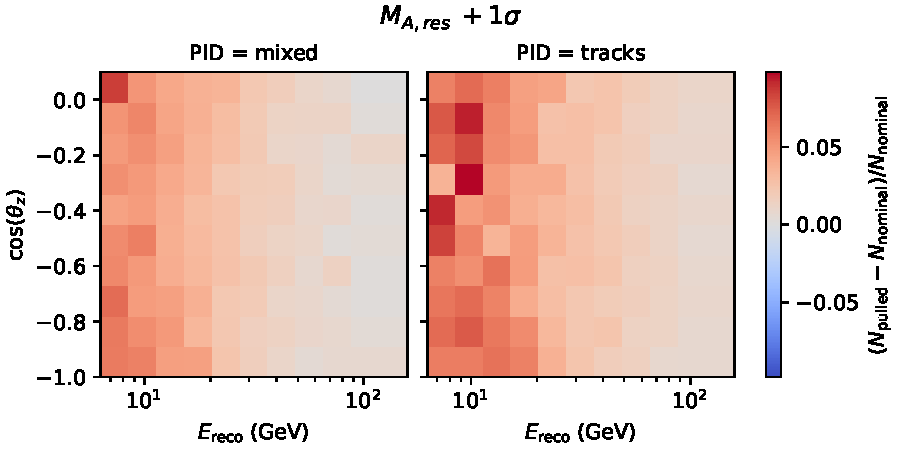
\includegraphics[width=0.99\textwidth,trim={0 0 0 0.6cm},clip]{figures/measurement/systematics/xsec/Genie_Ma_RES.pdf}
        \caption{GENIE $M_{A}^\mathrm{RES}$}
    \end{subfigure}
    \begin{subfigure}[t]{0.9\textwidth}
        \centering
        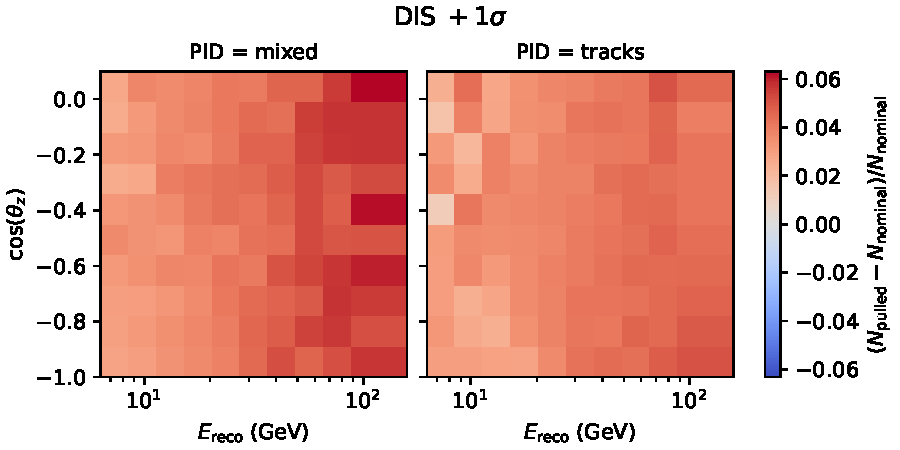
\includegraphics[width=0.99\textwidth,trim={0 0 0 0.6cm},clip]{figures/measurement/systematics/xsec/dis_csms.pdf}
        \caption{DIS CSMS}
    \end{subfigure}
  \caption{Fractional difference in event rates between (top )$M_{A}^\mathrm{RES}$ (bottom) dis$\_$csms at 1$\sigma$ and at nominal value for both PID bins.
  \label{fig:template_xsecsyst}}
\end{figure}

The uncertainty on the DIS cross-section is primarily given by the disagreement in DIS calculation between CSMS\cite{csms-xsec} and GENIE\cite{Andreopoulos:2015wxa} cross-sections at energies above 100~GeV.
This analysis includes a parameter that interpolates between these two calculations with a linear extrapolation to energies below 100~GeV.
The bottom panel of \reffig{template_xsecsyst} illustrates an example of the varying this parameter, DIS, on the final level sample.
As expected, the impact of the parameter is largest in the highest energy bins.
There is an additional uncertainty of 20\% on the normalization of NC events to account for uncertainties of the hadronization process and the Weinberg angle in line with previous oscillation studies\cite{Aartsen_2018}.

\subsection{Atmospheric muons}
The offline filter steps described in section~\ref{sec:offline-filter} decrease the rate of atmospheric muons by several orders of magnitude as events pass through each of its stages.
This makes it challenging to produce a sufficiently large amount of simulated muon events to accurately estimate the expected background at the final level.
To overcome this challenge, two separate muon simulation sets are produced, one of which is used to tune the lower level (up to L4) offline filters and the other is used to estimate muon background at levels L5 and above.

For both sets, atmospheric muons are generated on the surface of a cylinder encompassing the entire IceCube detector with a radius of 800~m and a height of 1600~m.
Positions and directions of muons interacting in the detector are sampled using parametrized tables based on the approach described in \sidecite{BECHERINI20061}.
These tables are tuned to approximate the output of a detailed \textsc{CORSIKA}\sidecite{Heck1998CORSIKAAM} simulation of cosmic ray interactions and subsequent shower production using the cosmic ray flux model described in \sidecite{Gaisser:2011klf} and the \textsc{SIBYLL 2.1}\sidecite{sibyll} hadronic interaction model.
This flux is also used to weight simulated muon events and is distinct from the flux model used to weight neutrino events.
For the simulations used to tune the lower selection levels, the muon energy is sampled from a power law with a spectral index of -3 and all events are accepted to cover the entire IceCube array.
To produce the simulation that is used starting at the L5 trigger level, muons are only accepted if they intersect an inner cylinder centered in the DeepCore fiducial volume with a radius of 180~m and a height of 400~m.
Furthermore, muons are rejected based on a KDE estimate of the muon density in energy and zenith angle at the L5 filter level.
In this way, the sampling preferably produces such muon events that have a higher chance of passing the offline filtering up to L5, which greatly improves the efficiency of the simulation production.

After the position, direction and energy for a muon has been sampled, its propagation and photon production is simulated using \textsc{PROPOSAL} in just the same way as any muon that is produced in neutrino interaction would be.

\subsubsection{Muon Uncertainty}
\label{sec:atm-muons-systematic}
Because the muon background contamination is cut to only $\sim$2\% at the final level of the event selection (see \refsec{final-sample-binning}), the impact of muon systematic uncertainties is generally small.
Only the over-all scale is left as a free parameter in the analysis, its impact is shown in \reffig{weight-scale-syst}.
This scale also largely absorbs the effects of DOM efficiency uncertainties, since, to first order, an increase in DOM efficiency leads to a better muon rejection.
The spectral index of the muon flux has a very small effect far below the percent-level as shown in \reffig{delta-gamma-mu-syst} and is therefore not accounted for in the analysis.

\begin{figure}
    \centering
    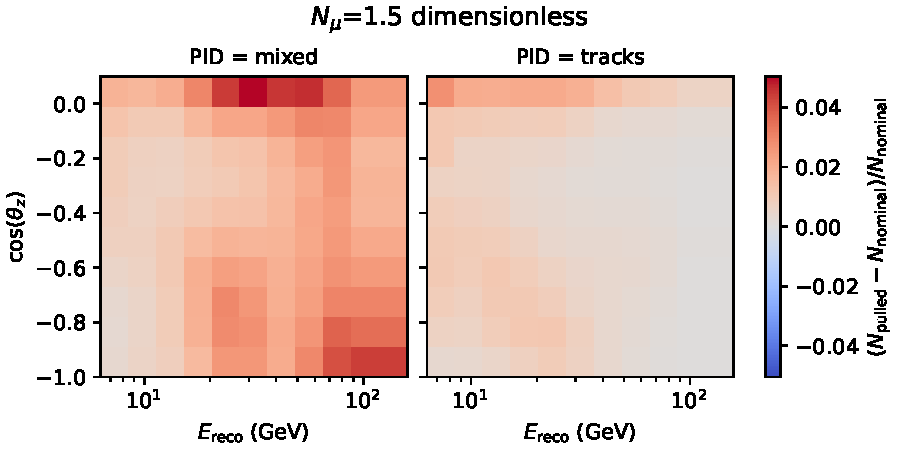
\includegraphics[width=0.7\textwidth,trim={0 0 0 0.6cm},clip]{figures/measurement/systematics/muons/weight_scale.pdf}
    \caption{Impact on the final histograms when the muon normalization is increased by 50\%. The largest impact is seen above the horizon in the mixed PID channel with a change in bin count of 5\%.}
    \label{fig:weight-scale-syst}
\end{figure}

\begin{figure}
    \centering
    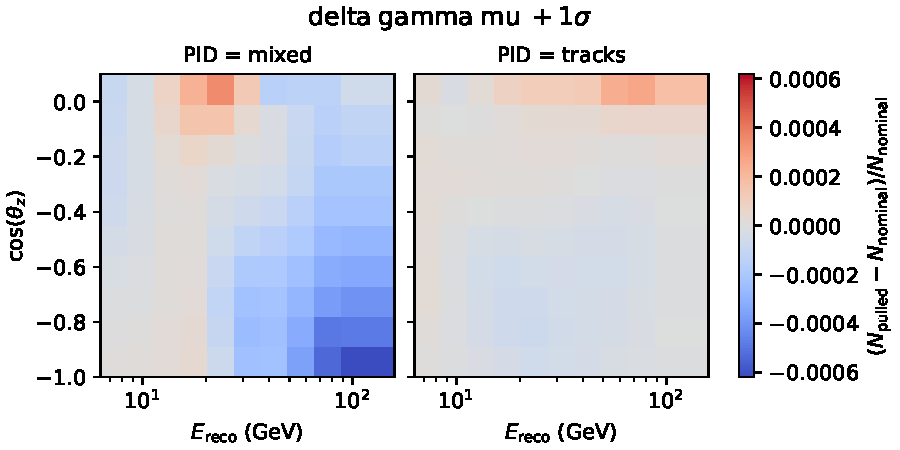
\includegraphics[width=0.7\textwidth,trim={0 0 0 0.6cm},clip]{figures/measurement/systematics/muons/delta_gamma_mu.pdf}
    \caption{Impact on the final histograms when the muon spectral index is increased by $1\sigma$.}
    \label{fig:delta-gamma-mu-syst}
\end{figure}

\subsection{Photon Propagation}
\label{sec:photon-propagation}

Photons are individually traced through the ice using the \textsc{clsim}\cite{clsim} package, which is a GPU-accelerated \textsc{OpenCL} re-implementation of the Photon-Propagation Code\sidecite{ppc}.
 The ice is modeled as 10~m thick layers with individual scattering and absorption lengths that are shown in \reffig{spice-model}.
The ice model used for the simulation in this work, also referred to as \emph{South Pole ICE (SPICE)}\sidecite{flasher_calibration}, incorporates the fact that the ice layers are slightly tilted with respect to the vertical axis, and that scattering and absorption strengths are not uniform as a function of azimuth.
For every photon, \textsc{clsim} first samples the absorption length from an exponential distribution whose expectation value is the absorption length of the current layer.
It then propagates all photons in parallel steps, where every step corresponds to one scattering event and the step length is sampled from an exponential distribution where the expectation value is the scattering length of the current layer.
The scattering angle is then sampled from a mixture of a Henyey-Greenstein distribution and a simplified Mie scattering distribution, where the shape parameters of these distributions have previously been calibrated using the in-situ LED calibration system\cite{flasher_calibration}.
Each photon stops when it has either reached its total absorption length or if it has intersected a DOM.
After all photons have either been absorbed or reached a sensor, the simulations stops and passes the photons that reached a sensor on to the next step simulating the detector response.

\begin{figure}
    \centering
    %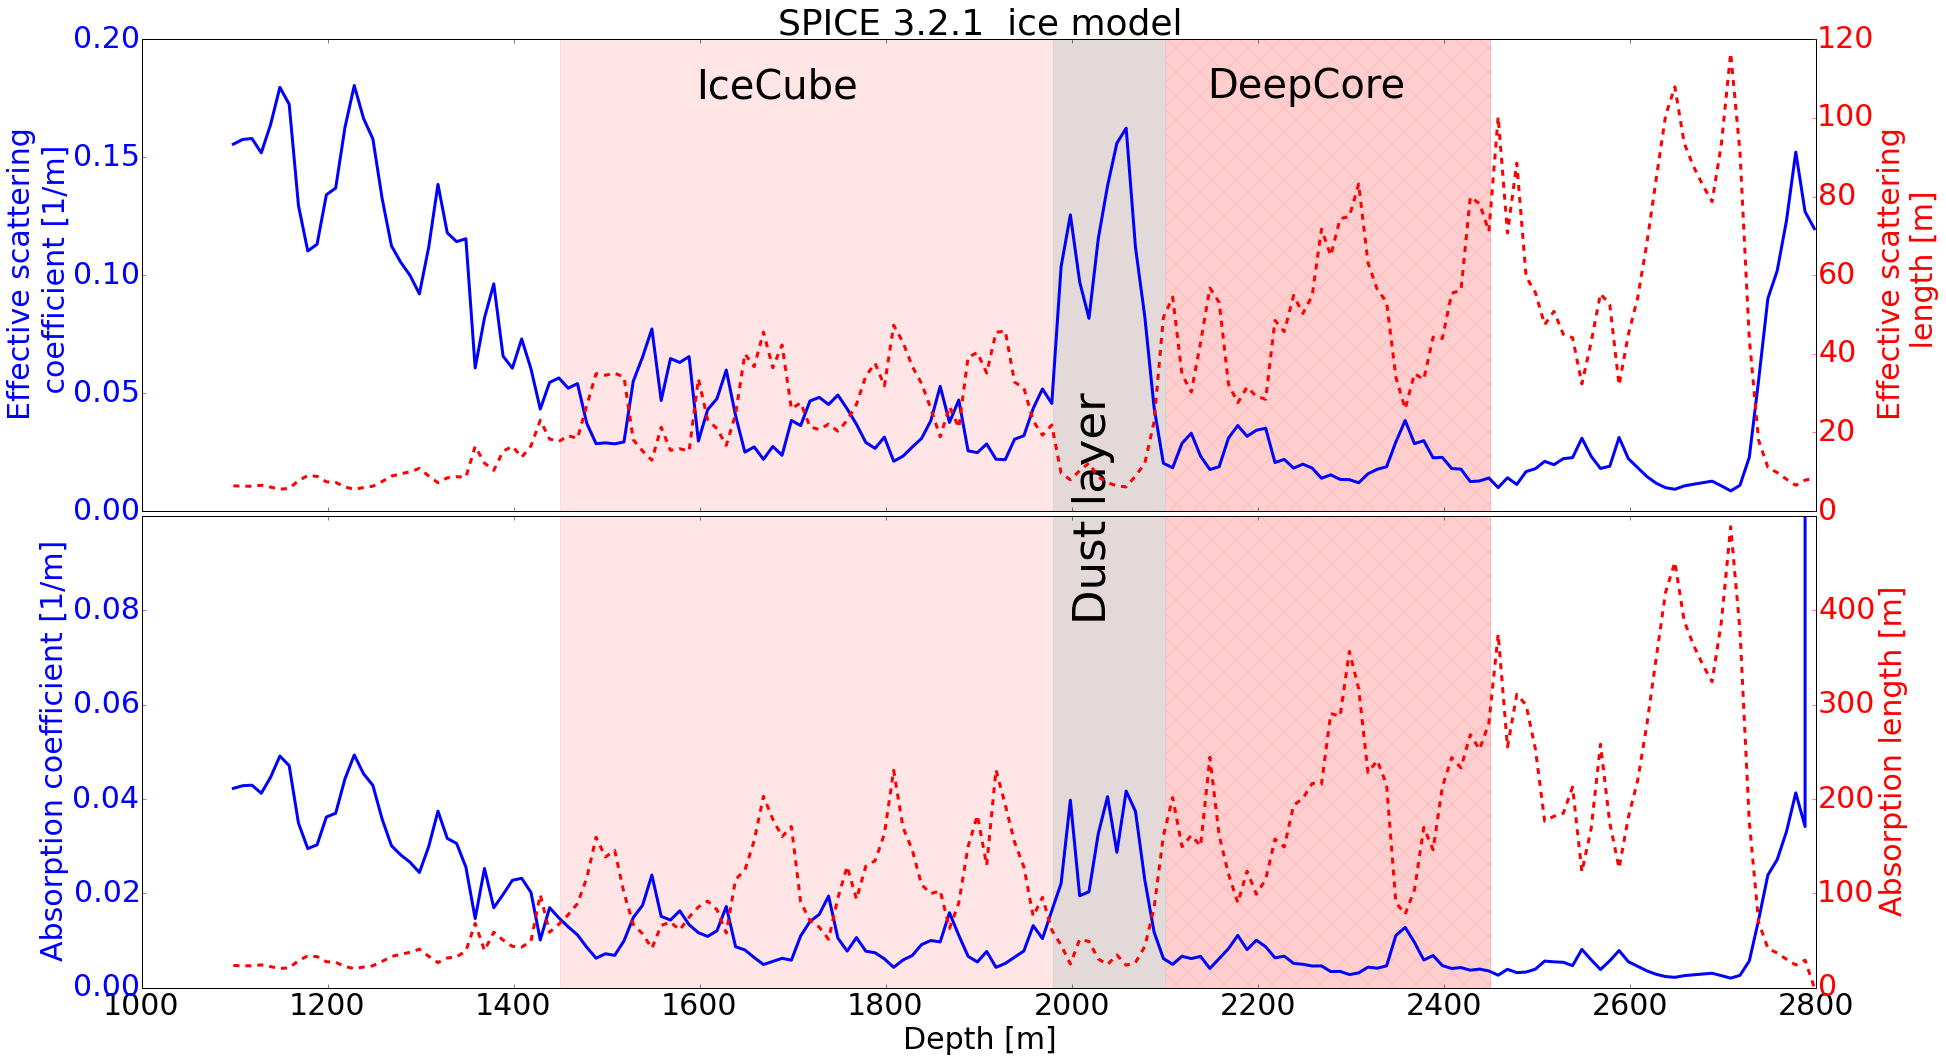
\includegraphics[width=0.9\linewidth]{figures/icecube/ice/Spice3.2.1_layered_scatt_abs_withlength_annotated.png}
    \tikzsetnextfilename{spice_model}%
\begin{tikzpicture}
% let both axes use the same layers
\pgfplotsset{set layers}

\pgfplotstableread{figures/icecube/ice/spice_model/spice_3.2.1/icemodel.dat}\table

\begin{axis}[
    scale only axis,
    width=0.7\linewidth,
    height=0.5\linewidth,
    xmin=1100,xmax=2900,
    xticklabel style={/pgf/number format/.cd,1000 sep={}},
    axis y line*=left, % the '*' avoids arrow heads
    ymin=0,
    enlarge y limits=true,
    xlabel=depth (m),
    ylabel=Scattering length (m),
]
    \addplot[black, thick] table [x index=0, y expr=1 / \thisrowno{1}] \table;
    
    % dust layer
    \draw [name path=dust layer top, gray, thin] (2000, \pgfkeysvalueof{/pgfplots/ymin}) -- (2000, \pgfkeysvalueof{/pgfplots/ymax}); 
    \draw [name path=dust layer bottom, gray, thin] (2100, \pgfkeysvalueof{/pgfplots/ymin}) -- node[near end, sloped, above, black, font=\footnotesize\sffamily] {dust layer} (2100, \pgfkeysvalueof{/pgfplots/ymax});
    \addplot [gray, opacity=0.4] fill between [of=dust layer top and dust layer bottom];
    
    % IceCube
    \draw [name path=icecube top, gray, thin] (1450, \pgfkeysvalueof{/pgfplots/ymin}) -- (1450, \pgfkeysvalueof{/pgfplots/ymax}); 
    \draw [name path=icecube bottom, gray, thin] (2000, \pgfkeysvalueof{/pgfplots/ymin}) -- (2000, \pgfkeysvalueof{/pgfplots/ymax});
    \node[anchor=south, black, font=\footnotesize\sffamily] at (1750, 110) {IceCube\strut};
    \addplot [gray, opacity=0.2] fill between [of=icecube top and icecube bottom];
    
    % DeepCore
    \draw [name path=deepcore top, gray, thin] (2100, \pgfkeysvalueof{/pgfplots/ymin}) -- (2100, \pgfkeysvalueof{/pgfplots/ymax}); 
    \draw [name path=deepcore bottom, gray, thin] (2450, \pgfkeysvalueof{/pgfplots/ymin}) -- (2450, \pgfkeysvalueof{/pgfplots/ymax});
    \node[anchor=south, black, font=\footnotesize\sffamily] at (2270, 110) {DeepCore\strut};
    \addplot [gray, opacity=0.1] fill between [of=deepcore top and deepcore bottom];
    
\end{axis}

\begin{axis}[
    orange,
    scale only axis,
    width=0.7\linewidth,
    height=0.5\linewidth,
    xmin=1100,xmax=2900,
    axis y line*=right,
    axis x line=none,
    ymin=0,
    enlarge y limits=true,
    ylabel=Absorption length (m),
]
    \addplot[orange, thick] table [x index=0, y expr=1 / \thisrowno{2}] \table;

\end{axis}

\end{tikzpicture}

    \caption{Scattering and absorption lengths as a function of depth in the South Pole Ice (SPICE) model that is used to produce the simulation for this work.}
    \label{fig:spice-model}
\end{figure}


\subsection{Simulation of Detector Response}
\label{sec:sim-detector-response}
After the photons have reached the surface of the optical sensors, the simulation determines for each one if it is converted into a Monte-Carlo photo-electron (MCPE).
The probability that this occurs depends on the wavelength-dependent sensitivity of the DOM, as well as the angular acceptance.
The angular acceptance not only depends on the geometry of the DOM itself, but also incorporates the effect of the re-frozen column of ice at the center of each bore hole.
If a photon is accepted and converted into an MCPE, the next step is to simulate how much charge would be measured by the PMT inside the DOM as a response.
The charge is drawn from a combination of a normal distribution and two exponential distributions whose parameters have been calibrated \emph{in-situ} to match the observed charge distribution in each individual DOM\sidecite{ic_spe_20}.
This distribution, also referred to as the Single Photo-Electron (SPE) template, is shown in \reffig{spe-templates}.
The MCPEs with the samples charge are then converted into simulated waveforms for the ATWD and fADC readouts which are then passed into the data processing chain starting from the \emph{wavedeform} algorithm described in Section~\ref{sec:dom-daq}.
From there, the simulated events pass through all the same trigger and filter steps that are described in Section~\ref{sec:data-processing}.

\begin{figure}
    \centering
    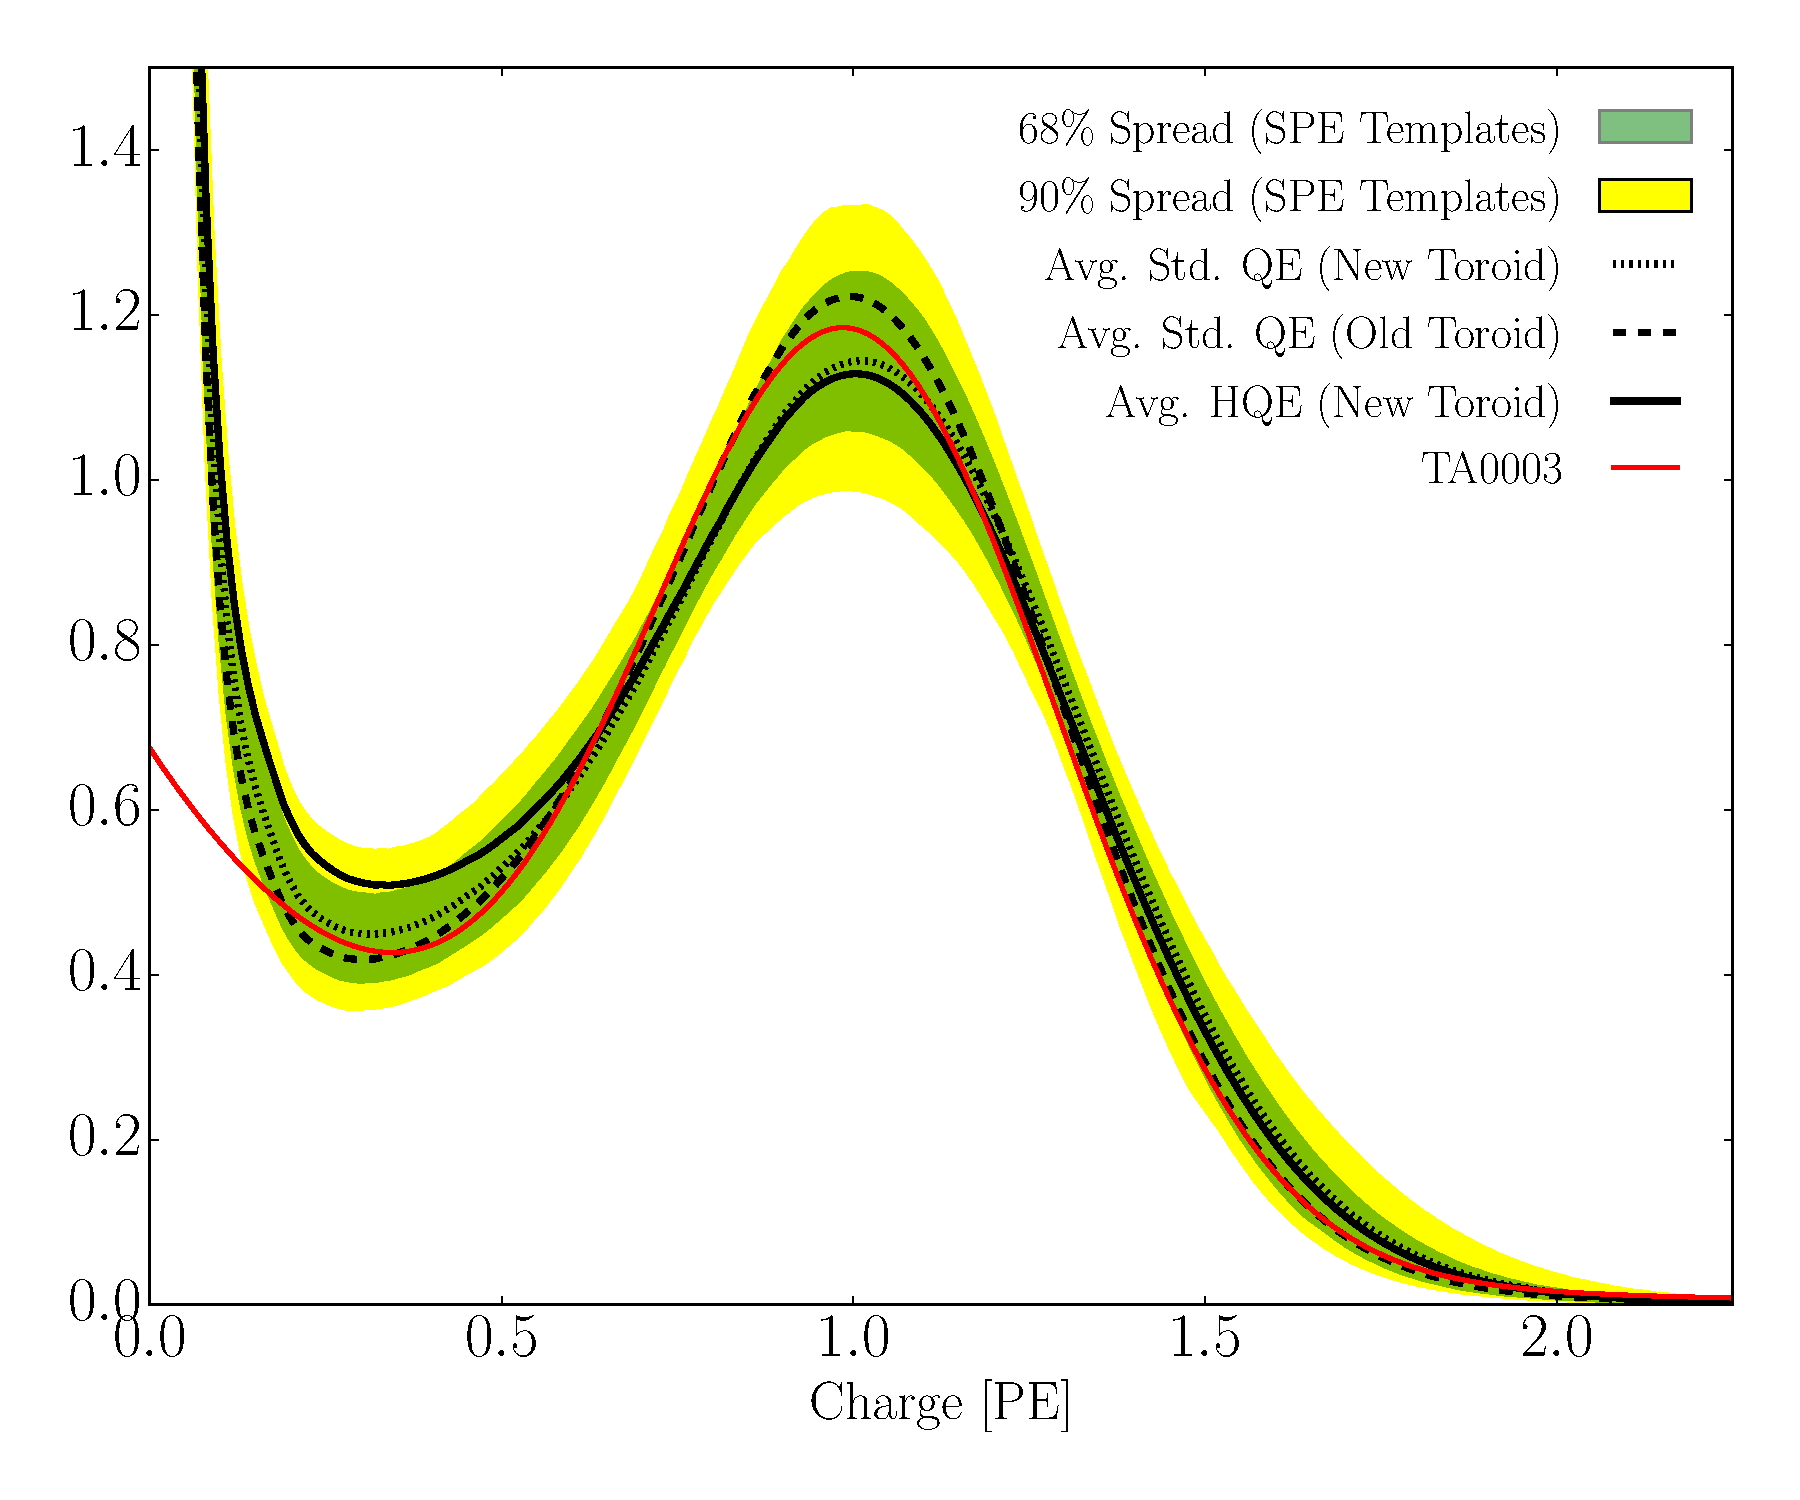
\includegraphics[width=0.8\linewidth]{figures/icecube/detector_response/SPE_TA003_2.pdf}
    \caption{The green (yellow) regions show the 68\% (90\%) spread in the SPE charge templates for a given charge.  Superimposed are the average SPE charge templates for the variety of hardware configurations shown in the black dotted, dashed, and solid lines. The TA0003 distribution, shown in red, originates from laboratory measurements. Figure taken from \cite{ic_spe_20}.}
    \label{fig:spe-templates}
\end{figure}

\subsubsection{Detector Noise}

\begin{margintable}
\caption{\label{tab:vuvuzela_params} Parameters used in the noise simulation. Typical values taken from \cite{Michael_Larson_masters}, actual values are fit for each DOM individually.}
    \begin{tabular}{lc}\toprule
        \textbf{Parameter} & \textbf{Typical value} \\ \midrule
        Therm. rate &  $\lambda_\mathrm{th}\approx \SI{20}{\hertz}$ \\
        Decay rate &  $\lambda_\mathrm{dec}\approx \SI{250}{\hertz}$ \\
        Decay hits &  $\eta\approx 8$ \\
        Decay $\mu$ &  $\log_{10}(\frac{\mu}{\si{\nano\second}}) \approx -6$\\
        Decay $\sigma$ &  $\log_{10}(\frac{\sigma}{\si{\nano\second}}) \approx 2.7$ \\ \bottomrule
    \end{tabular}
\end{margintable}
In addition to Cherenkov photons induced by relativistic charged particles in the ice, IceCube detects photons from radioactive decays inside the glass housing of the DOMs and PMTs that are simulated using the \emph{Vuvuzela} module\sidecite{Michael_Larson_masters}\sidecite{Michael_Larson_phd}.
These "noise" MCPEs are simulated parametrically by sampling their times from distributions that take both thermal and non-thermal noise components into account. The thermal component comes from uncorrelated photons and PMT dark noise and is modeled as a Poisson process with a constant rate.
The non-thermal component comes from correlated bursts of photons that are produced by radioactive decays.
To simulate it, decay times are first drawn from a Poisson process with a constant rate, and the number of photons produced in each decay is sampled from a Poisson distribution.
The time differences between the non-thermal MCPEs produced by each decay are then sampled from a Log-Gaussian distribution.
This simulation method has five free parameters listed in \reftab{vuvuzela_params} that are calibrated \emph{in-situ} for every DOM.
All thermal and non-thermal MCPEs are injected into each simulated event together with the MCPEs from photons and passed into the rest of the simulation chain.
% \begin{margintable}
% \caption{\label{tab:vuvuzela_params} Parameters used in the noise simulation. }
%     \begin{tabular}{lcc}\toprule
%         \textbf{Parameter} & \textbf{Designation} & \textbf{Unit} \\ \midrule
%         Thermal rate & $\lambda_{Th}$ & $s^{-1}$ \\
%         Decay rate & $\lambda_{Decay}$ & $s^{-1}$ \\
%         Scintillation hits & $\eta_{Scint}$ & hits \\
%         Scintillation mean & $\mu_{Scint}$ & $\log_{10} (ns) $\\
%         Scintillation sigma & $\sigma_{Scint}$ &  $\log_{10} (ns) $ \\ \bottomrule
%     \end{tabular}
% \end{margintable}




\section{Data Processing}
\label{sec:data-processing}

\subsection{Trigger}
As described in section \ref{sec:dom-daq}, the high-frequency ATWD waveform digitization in each DOM is triggered when it and its adjacent or next-to-adjacent neighbors on the same string record a voltage of at least 0.25 PE-equivalent within a $\pm$1~$\mu$s time window, which is referred to as the Hard Local Coincidence (HLC) condition.
Data acquisition for DeepCore is triggered when this condition is fulfilled for at least three DOMs inside the DeepCore fiducial volume within a $\pm$2.5~$\mu$s window.
If this condition is met, the waveforms for all DOMs that have observed voltages of at least 0.25~PE within a $\pm$10~$\mu$s time window centered around the trigger time are recorded.
A DOM that is included in this readout but for which the HLC condition has not been met is said to fulfill the \emph{Soft Local Coincidence} (SLC) condition.
The DeepCore trigger rate is less than 10~Hz and will trigger on $\sim$70\% of $\nu_\mu$ events at 10~GeV and >90\% of $\nu_\mu$ events at 100~GeV\cite{DeepCore}.

\subsection{Online Filter}
\begin{marginfigure}
    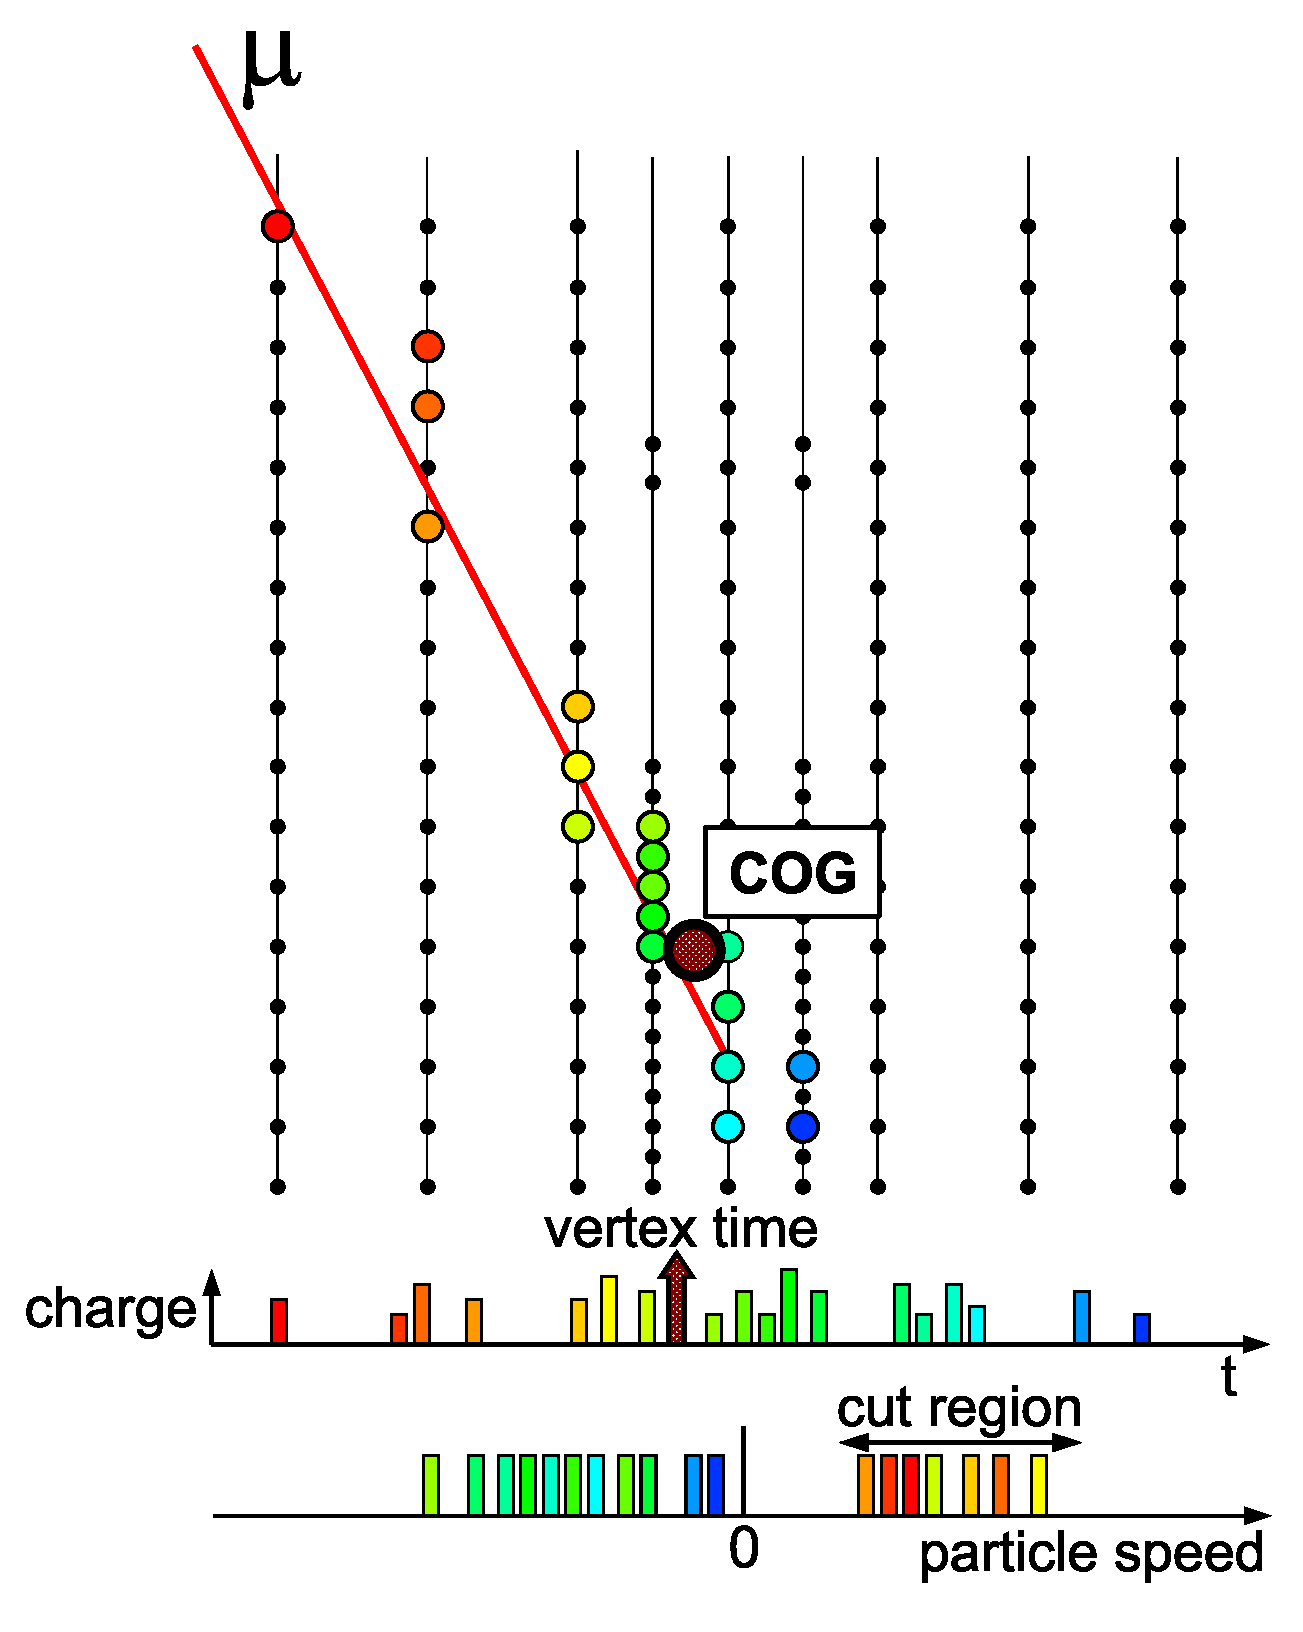
\includegraphics[width=\textwidth]{figures/icecube/eventviews/FilterDiagram.pdf}
    \caption{Example of an event that would be rejected by the online filter algorithm. DOMs that have observed light are highlighted in color depending on time from red (early hits) to blue (late hits). DOMs that have not observed any light are shown as black dots. Figure taken from \cite{DeepCore}.}
    \label{fig:online-filter-event}
\end{marginfigure}
Once the trigger condition is met, the recorded waveforms within the trigger window are converted into reconstructed pulses and are then passed into a set of \emph{online} filters (i.e.
filters running on hardware at the Pole).
These filters are each designed to select events that are relevant to different physics measurements that are performed within the IceCube collaboration.
For the purposes of the analysis presented in this thesis, events are selected using the \emph{DeepCore filter}\sidecite{DeepCore}.
This filter is designed to select events that start inside the DeepCore fiducial volume and to reject those that are consistent with muons entering the detector from the outside.
The filter splits the observed series of hits between those hits that fall within the DeepCore fiducial volume and those outside of it.
It then estimates the "center of gravity" (COG) in space and time of the hits inside the fiducial volume and then calculates the velocity that a signal would have to travel from each hit occurring outside the fiducial volume to coincide with the COG.
If this velocity is close to the speed of light (between $0.25\;\mathrm{ns/s}$ and $0.4\;\mathrm{ns/s}$) for at least one hit, the event is rejected because it is consistent with a muon traveling through the veto region and entering DeepCore.
\reffig{online-filter-event} shows an example of an event that would be rejected by the online filter.
Only events that pass the trigger and filter conditions are sent north via satellite for further \emph{offline} filtering.

\subsection{Offline Filter}
\label{sec:offline-filter}
The offline filter is separated into subsequently applied \emph{levels}, referred to as L3, L4 and L5, where each level reduces the amount of background (atmospheric muons and noise) by approximately an order of magnitude while keeping most of the DeepCore starting events that are the target of the selection.

\subsubsection{Level 3}
At the lowest offline filter level, L3, cuts are applied to simple variables that remove the most easily identifiable background events while using only few computational resources.
The variables aimed at cutting noise consist mainly of different DOM hit counts within hit series to which noise cleaning algorithms have been applied.
The cuts aimed at removing muons consist of conditions on the number of hits in the veto region and conditions on the vertical position of the first HLC hit.
The distributions for two of the variables used in the L3 filter are shown in \reffig{l3-cut-vars}.
It is apparent from the distributions that there is a significant population of events in data with large values of the plotted variable that does not exist in simulation.
These events are discarded, improving the agreement between the data and simulation for events that pass the L3 filter.
% \begin{figure}
%     \centering
%     \begin{tikzpicture}

    \definecolor{black}{RGB}{0,0,0}
    \definecolor{orange}{RGB}{230, 159, 0}
    \definecolor{skyblue}{RGB}{86, 180, 233}
    \definecolor{bluishgreen}{RGB}{0, 158, 115}
    \definecolor{yellow}{RGB}{240, 228, 66}
    \definecolor{blue}{RGB}{0, 114, 178}
    \definecolor{vermilion}{RGB}{213, 94, 0}
    \definecolor{reddishpurple}{RGB}{204, 121, 167}

    \definecolor{lightgray204}{RGB}{204,204,204}


    \pgfplotstableread{figures/icecube/selection/Level3/DCFiducialHits_level3_data_mc_hists.csv}\table
    \begin{groupplot}[
        xmajorgrids, ymajorgrids,
        width=\linewidth,
        group/.cd,
        group size=1 by 2,
        xticklabels at=edge bottom,
        vertical sep=10pt
    ]
    \nextgroupplot[
        height=0.6\linewidth,
        legend cell align={left},
        legend columns=4,
        legend style={
          fill opacity=0.8,
          draw opacity=1,
          text opacity=1,
          at={(0.5,0.91)},
          anchor=north,
          draw=lightgray204
        },
        ymode=log,
        ymin=0.0001, ymax=1000.0,
        ylabel={rate (Hz)},
    ]
    \addplot[const plot, bluishgreen, thick] table [x=bin_edges, y=nuex100] from \table;
    \addlegendentry{$\nu_e + \bar{\nu}_e$ x100}
    \addplot[const plot, vermilion, thick] table [x=bin_edges, y=numux100] from \table;
    \addlegendentry{$\nu_\mu + \bar{\nu}_\mu$ x100}
    \addplot[const plot, yellow, thick] table [x=bin_edges, y=nutaux100] from \table;
    \addlegendentry{$\nu_\tau + \bar{\nu}_\tau$ x100}
    \addplot[const plot, orange, thick] table [x=bin_edges, y=muon] from \table;
    \addlegendentry{atm. muons}
    \addplot[const plot, skyblue, thick] table [x=bin_edges, y=noise] from \table;
    \addlegendentry{noise}
    \addplot[const plot, black, thick] table [x=bin_edges, y=total_mc] from \table;
    \addlegendentry{total MC}
    \addplot+[
        mark=*,
        mark options={scale=0.5, fill=black},
        black,
        only marks,
        error bars/.cd,
        x dir=none,
        y dir=both,
        y explicit
    ] table [x=bin_midpoints, y=data, y error=data__err]  from \table;
    \addlegendentry{data (2014)}


    \addplot[const plot, bluishgreen, thin, name path=nuex100_lo] table[x=bin_edges, y=nuex100__err_dn] from \table;
    \addplot[const plot, bluishgreen, thin, name path=nuex100_hi] table[x=bin_edges, y=nuex100__err_up] from \table;
    \addplot[bluishgreen,opacity=0.5] fill between[of = nuex100_lo and nuex100_hi];


    \addplot[const plot, vermilion, thin, name path=numux100_lo] table[x=bin_edges, y=numux100__err_dn] from \table;
    \addplot[const plot, vermilion, thin, name path=numux100_hi] table[x=bin_edges, y=numux100__err_up] from \table;
    \addplot[vermilion,opacity=0.5] fill between[of = numux100_lo and numux100_hi];


    \addplot[const plot, yellow, thin, name path=nutaux100_lo] table[x=bin_edges, y=nutaux100__err_dn] from \table;
    \addplot[const plot, yellow, thin, name path=nutaux100_hi] table[x=bin_edges, y=nutaux100__err_up] from \table;
    \addplot[yellow,opacity=0.5] fill between[of = nutaux100_lo and nutaux100_hi];


    \addplot[const plot, orange, thin, name path=muon_lo] table[x=bin_edges, y=muon__err_dn] from \table;
    \addplot[const plot, orange, thin, name path=muon_hi] table[x=bin_edges, y=muon__err_up] from \table;
    \addplot[orange,opacity=0.5] fill between[of = muon_lo and muon_hi];


    \addplot[const plot, skyblue, thin, name path=noise_lo] table[x=bin_edges, y=noise__err_dn] from \table;
    \addplot[const plot, skyblue, thin, name path=noise_hi] table[x=bin_edges, y=noise__err_up] from \table;
    \addplot[skyblue,opacity=0.5] fill between[of = noise_lo and noise_hi];


    \addplot[const plot, black, thin, name path=total_mc_lo] table[x=bin_edges, y=total_mc__err_dn] from \table;
    \addplot[const plot, black, thin, name path=total_mc_hi] table[x=bin_edges, y=total_mc__err_up] from \table;
    \addplot[black,opacity=0.5] fill between[of = total_mc_lo and total_mc_hi];


    \nextgroupplot[
        height=0.3\linewidth,
        ymin=0.5, ymax=2,
        ylabel={data/MC ratio},
    ]
    \addplot[const plot, black, thick] table[x=bin_edges, y=data_mc_ratio] from \table;


    \addplot[const plot, black, thin, name path=data_mc_ratio_lo] table[x=bin_edges, y=data_mc_ratio__err_dn] from \table;
    \addplot[const plot, black, thin, name path=data_mc_ratio_hi] table[x=bin_edges, y=data_mc_ratio__err_up] from \table;
    \addplot[black,opacity=0.5] fill between[of = data_mc_ratio_lo and data_mc_ratio_hi];
    \end{groupplot}
\end{tikzpicture}


%     \caption{DCFiducialHits}
%     \label{fig:l3-dc-fiducial-hits}
% \end{figure}
% \begin{figure}
%     \centering
%     %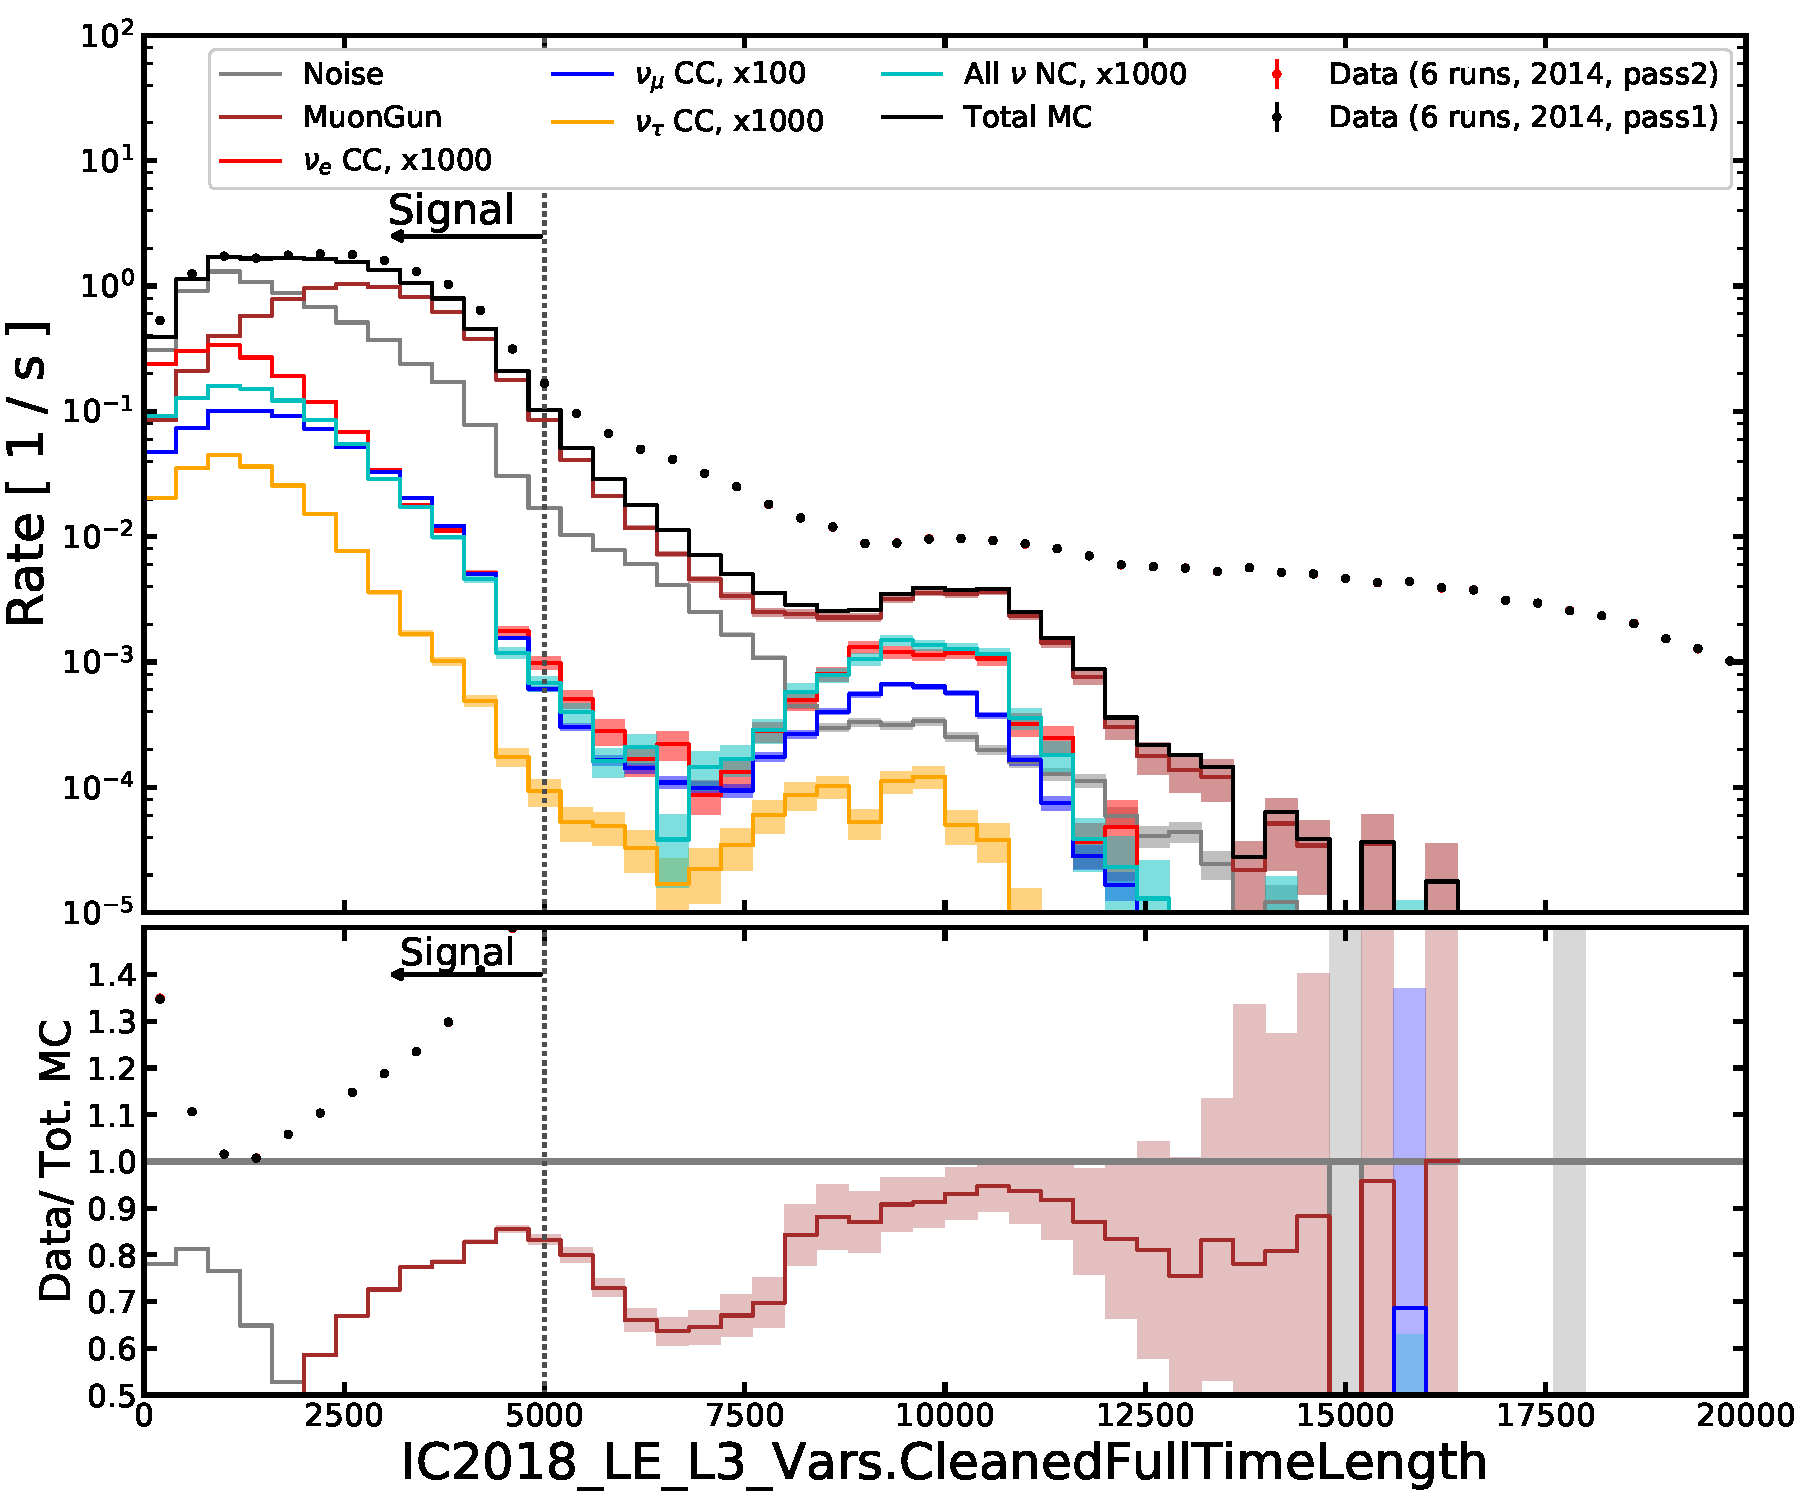
\includegraphics[width=7 cm]{figures/icecube/selection/IC2018_LE_L3_Vars_CleanedFullTimeLength.pdf}
%     \tikzsetnextfilename{l3_cleaned_full_time_length}%
\begin{tikzpicture}
    \pgfplotstableread{figures/icecube/selection/Level3/CleanedFullTimeLength_level3_data_mc_hists.csv}\table
    \begin{groupplot}[
        % xmin=0.0,xmax=25000.0,
        % this filter is applied to all x-coordinates in all plots!
        % Note that this filter would have to work on the *log* of the coordinates
        % if the x-axis was a log-axis (i.e. instead of scaling, you would shift).
        x filter/.expression={x*1e-3},
        xmin=0.0,xmax=25,
        xmajorgrids, ymajorgrids,
        width=0.45\linewidth,
        % The line below sets the position of the y-labels for all axes in
        % relative coordinates. Comment out to set positions automatically (which
        % may result in the "data/MC ratio" label being set a bit too far inside).
        ylabel style={at={(-0.15,0.5)}},
        group/.cd,
        group size=1 by 2,
        xticklabels at=edge bottom,
        vertical sep=10pt
        ]
    \nextgroupplot[
        height=0.35\linewidth,
        legend cell align={left},
        legend columns=4,
        legend to name=l3_vars_legend,
        legend style={
          at={(0.95,0.95)},
          anchor=north east,
        },
        ymode=log,
        % ymin=1e-05, ymax=1000.0,
        ymin=2e-5, ymax=5e2,
        ytick distance=1e1,
        ylabel={rate (Hz)},
        y filter/.expression={y < 1e-6 ? ln(1e-6) : ln(y)}
    ]
    % for some reason we called the column "muon", not "muons"...
    \ploterrorband[muon_color]{muon}{1}
    \addlegendentry{atm. muons}
    \ploterrorband[nue_color]{nue}{100}
    \addlegendentry{$\nu_e + \bar{\nu}_e$ x100}
    \ploterrorband[numu_color]{numu}{100}
    \addlegendentry{$\nu_\mu + \bar{\nu}_\mu$ x100}
    \ploterrorband[nutau_color]{nutau}{1000}
    \addlegendentry{$\nu_\tau + \bar{\nu}_\tau$ x1000}
    \ploterrorband[noise_color]{noise}{1}
    \addlegendentry{noise}
    \ploterrorband{total_mc}{1}
    \addlegendentry{total MC}

    \ploterrorbar{data}
    \addlegendentry{data (2014, 12 runs)}

    % draw cut
    % use "axis cs" to give coordinates in the data coordinate system!

    % \draw[thick,dashed] (axis cs:5000,1e-4) -- (axis cs:5000,100);
    % \draw[-stealth, very thick] (axis cs:5000,10)  -- node[anchor=south]{signal} (axis cs:1000,10);

    % since we scaled the coordnates to microseconds, we also need to use that for drawing
    \draw[thick,dashed] (axis cs:5,1e-6) -- (axis cs:5,100);
    \draw[-stealth, very thick] (axis cs:5,10)  -- node[anchor=south]{\footnotesize\sffamily signal} (axis cs:1,10);

    \nextgroupplot[
        height=0.2\linewidth,
        ymin=-0.1, ymax=2.85,
        ylabel=rate/total MC,
        xlabel={CleanedFullTimeLength ($\mu$s)}
    ]
   
    \ploterrorbar{data_mc_ratio}
    \plotratioerrorband[muon_color]{muon}{total_mc}
    \plotratioerrorband[nue_color]{nue}{total_mc}
    \plotratioerrorband[numu_color]{numu}{total_mc}
    \plotratioerrorband[nutau_color]{nutau}{total_mc}
    \plotratioerrorband[noise_color]{noise}{total_mc}
    
    \end{groupplot}
\end{tikzpicture}

%     \caption{Distribution of one of the variables used in the L3 offline filter, the time between the last hit and the first hit after noise cleaning. Histograms show the distributions in simulated data separated by particle and interaction type, data points with error bars show the distribution of real data. The bottom panel shows the ratio between data and simulation. Events falling on the "signal" side of the histogram are passed to the next filter level.}
%     \label{fig:l3-var-cleaned-full-time-length}
% \end{figure}

\begin{figure*}
    \centering
    \ref{l3_vars_legend}\par
    \tikzsetnextfilename{l3_cleaned_full_time_length}%
\begin{tikzpicture}
    \pgfplotstableread{figures/icecube/selection/Level3/CleanedFullTimeLength_level3_data_mc_hists.csv}\table
    \begin{groupplot}[
        % xmin=0.0,xmax=25000.0,
        % this filter is applied to all x-coordinates in all plots!
        % Note that this filter would have to work on the *log* of the coordinates
        % if the x-axis was a log-axis (i.e. instead of scaling, you would shift).
        x filter/.expression={x*1e-3},
        xmin=0.0,xmax=25,
        xmajorgrids, ymajorgrids,
        width=0.45\linewidth,
        % The line below sets the position of the y-labels for all axes in
        % relative coordinates. Comment out to set positions automatically (which
        % may result in the "data/MC ratio" label being set a bit too far inside).
        ylabel style={at={(-0.15,0.5)}},
        group/.cd,
        group size=1 by 2,
        xticklabels at=edge bottom,
        vertical sep=10pt
        ]
    \nextgroupplot[
        height=0.35\linewidth,
        legend cell align={left},
        legend columns=4,
        legend to name=l3_vars_legend,
        legend style={
          at={(0.95,0.95)},
          anchor=north east,
        },
        ymode=log,
        % ymin=1e-05, ymax=1000.0,
        ymin=2e-5, ymax=5e2,
        ytick distance=1e1,
        ylabel={rate (Hz)},
        y filter/.expression={y < 1e-6 ? ln(1e-6) : ln(y)}
    ]
    % for some reason we called the column "muon", not "muons"...
    \ploterrorband[muon_color]{muon}{1}
    \addlegendentry{atm. muons}
    \ploterrorband[nue_color]{nue}{100}
    \addlegendentry{$\nu_e + \bar{\nu}_e$ x100}
    \ploterrorband[numu_color]{numu}{100}
    \addlegendentry{$\nu_\mu + \bar{\nu}_\mu$ x100}
    \ploterrorband[nutau_color]{nutau}{1000}
    \addlegendentry{$\nu_\tau + \bar{\nu}_\tau$ x1000}
    \ploterrorband[noise_color]{noise}{1}
    \addlegendentry{noise}
    \ploterrorband{total_mc}{1}
    \addlegendentry{total MC}

    \ploterrorbar{data}
    \addlegendentry{data (2014, 12 runs)}

    % draw cut
    % use "axis cs" to give coordinates in the data coordinate system!

    % \draw[thick,dashed] (axis cs:5000,1e-4) -- (axis cs:5000,100);
    % \draw[-stealth, very thick] (axis cs:5000,10)  -- node[anchor=south]{signal} (axis cs:1000,10);

    % since we scaled the coordnates to microseconds, we also need to use that for drawing
    \draw[thick,dashed] (axis cs:5,1e-6) -- (axis cs:5,100);
    \draw[-stealth, very thick] (axis cs:5,10)  -- node[anchor=south]{\footnotesize\sffamily signal} (axis cs:1,10);

    \nextgroupplot[
        height=0.2\linewidth,
        ymin=-0.1, ymax=2.85,
        ylabel=rate/total MC,
        xlabel={CleanedFullTimeLength ($\mu$s)}
    ]
   
    \ploterrorbar{data_mc_ratio}
    \plotratioerrorband[muon_color]{muon}{total_mc}
    \plotratioerrorband[nue_color]{nue}{total_mc}
    \plotratioerrorband[numu_color]{numu}{total_mc}
    \plotratioerrorband[nutau_color]{nutau}{total_mc}
    \plotratioerrorband[noise_color]{noise}{total_mc}
    
    \end{groupplot}
\end{tikzpicture}

    \tikzsetnextfilename{l3_vertex_guess_z}%
\begin{tikzpicture}
    \pgfplotstableread{figures/icecube/selection/Level3/VertexGuessZ_level3_data_mc_hists.csv}\table
    \begin{groupplot}[
        xmin=-600,xmax=600,
        xmajorgrids, ymajorgrids,
        width=0.45\linewidth,
        % The line below sets the position of the y-labels for all axes in 
        % relative coordinates. Comment out to set positions automatically (which 
        % may result in the "data/MC ratio" label being set a bit too far inside).
        ylabel style={at={(-0.15,0.5)}},
        group/.cd,
        group size=1 by 2,
        xticklabels at=edge bottom,
        vertical sep=10pt
        ]
    \nextgroupplot[
        height=0.35\linewidth,
        legend cell align={left},
        legend columns=1,
        legend to name=l3_vars_legend_vertex_guess,
        ymode=log,
        ymin=2e-5, ymax=5e2,
        ytick distance=1e1,
        ylabel={rate (Hz)},
        y filter/.expression={y < 1e-6 ? ln(1e-6) : ln(y)}
    ]
    % for some reason we called the column "muon", not "muons"...
    \ploterrorband[muon_color]{muon}{1}
    \addlegendentry{atm. muons}
    \ploterrorband[nue_color]{nue}{100}
    \addlegendentry{$\nu_e + \bar{\nu}_e$ x100}
    \ploterrorband[numu_color]{numu}{100}
    \addlegendentry{$\nu_\mu + \bar{\nu}_\mu$ x100}
    \ploterrorband[nutau_color]{nutau}{1000}
    \addlegendentry{$\nu_\tau + \bar{\nu}_\tau$ x1000}
    \ploterrorband[noise_color]{noise}{1}
    \addlegendentry{noise}
    \ploterrorband{total_mc}{1}

    \ploterrorbar{data}
    \addlegendentry{data (2014, 12 runs)}

    \draw[thick,dashed] (axis cs:-120,1e-6) -- (axis cs:-120,100);
    \draw[-stealth, very thick] (axis cs:-120,5)  -- node[anchor=south]{\footnotesize\sffamily signal} (axis cs:-400,5);

    \nextgroupplot[
        height=0.2\linewidth,
        ymin=0.5, ymax=4,
        ylabel={data/MC ratio},
        xlabel={first HLC z-position}
    ]
    \ploterrorband{data_mc_ratio}{1}
    \end{groupplot}
\end{tikzpicture}


    \caption{Distribution of one of the variables used in the L3 offline filter, the time between the last hit and the first hit after noise cleaning (left) and the z-position of the first HLC hit (right). Histograms show the distributions in simulated data separated by event type, data points with error bars show the distribution of real data. The bottom panel shows the ratio between data and simulation. Events falling on the "signal" side of the histogram are passed to the next filter level.}
    \label{fig:l3-cut-vars}
\end{figure*}

\subsubsection{Level 4}
\label{sec:level4-selection}
In the next level, L4, more advanced selections based on the output of Boosted Decision Trees (BDTs) are applied, with a separately trained BDT for noise and muon rejection, respectively.
The output of each BDT is a probability score between zero (background-like) and one (signal-like).
The first BDT to be evaluated is the one used to reject pure noise events.
Its inputs consist of hit counts in cleaned hit series and variables that characterize the geometric and temporal spread of the observed hits, such as the full width half maximum (FWHM) of the hit times.
The BDT is trained using simulated pure noise and neutrino events.
An event passes the noise filter if the BDT score is above 0.7, which reduces the number of pure noise events by two orders of magnitude from 36.6~mHz to approximately 0.3~mHz.
Passing events are passed into the second BDT that is used to reject atmospheric muons.
This BDT also takes simple variables as its input that consist mostly of different veto hit counts and variables that characterize the distribution of z-coordinates of the observed hits as well as their radial distance with respect to the center of the DeepCore fiducial volume.
In contrast to the noise BDT, however, the muon BDT is trained using real data and simulated neutrino events, with the goal of rejecting data events.
This is possible because the data sample consists to 99\% of atmospheric muons at this stage of the event selection.
Events pass the L4 muon cut if the output score of the muon BDT is greater than 0.65, removing 94\% of all muon events while keeping 87\% of all neutrinos.
The distributions of the output scores of both BDTs are shown in \reffig{l4-bdt-output}.
\begin{figure*}
    \centering
    %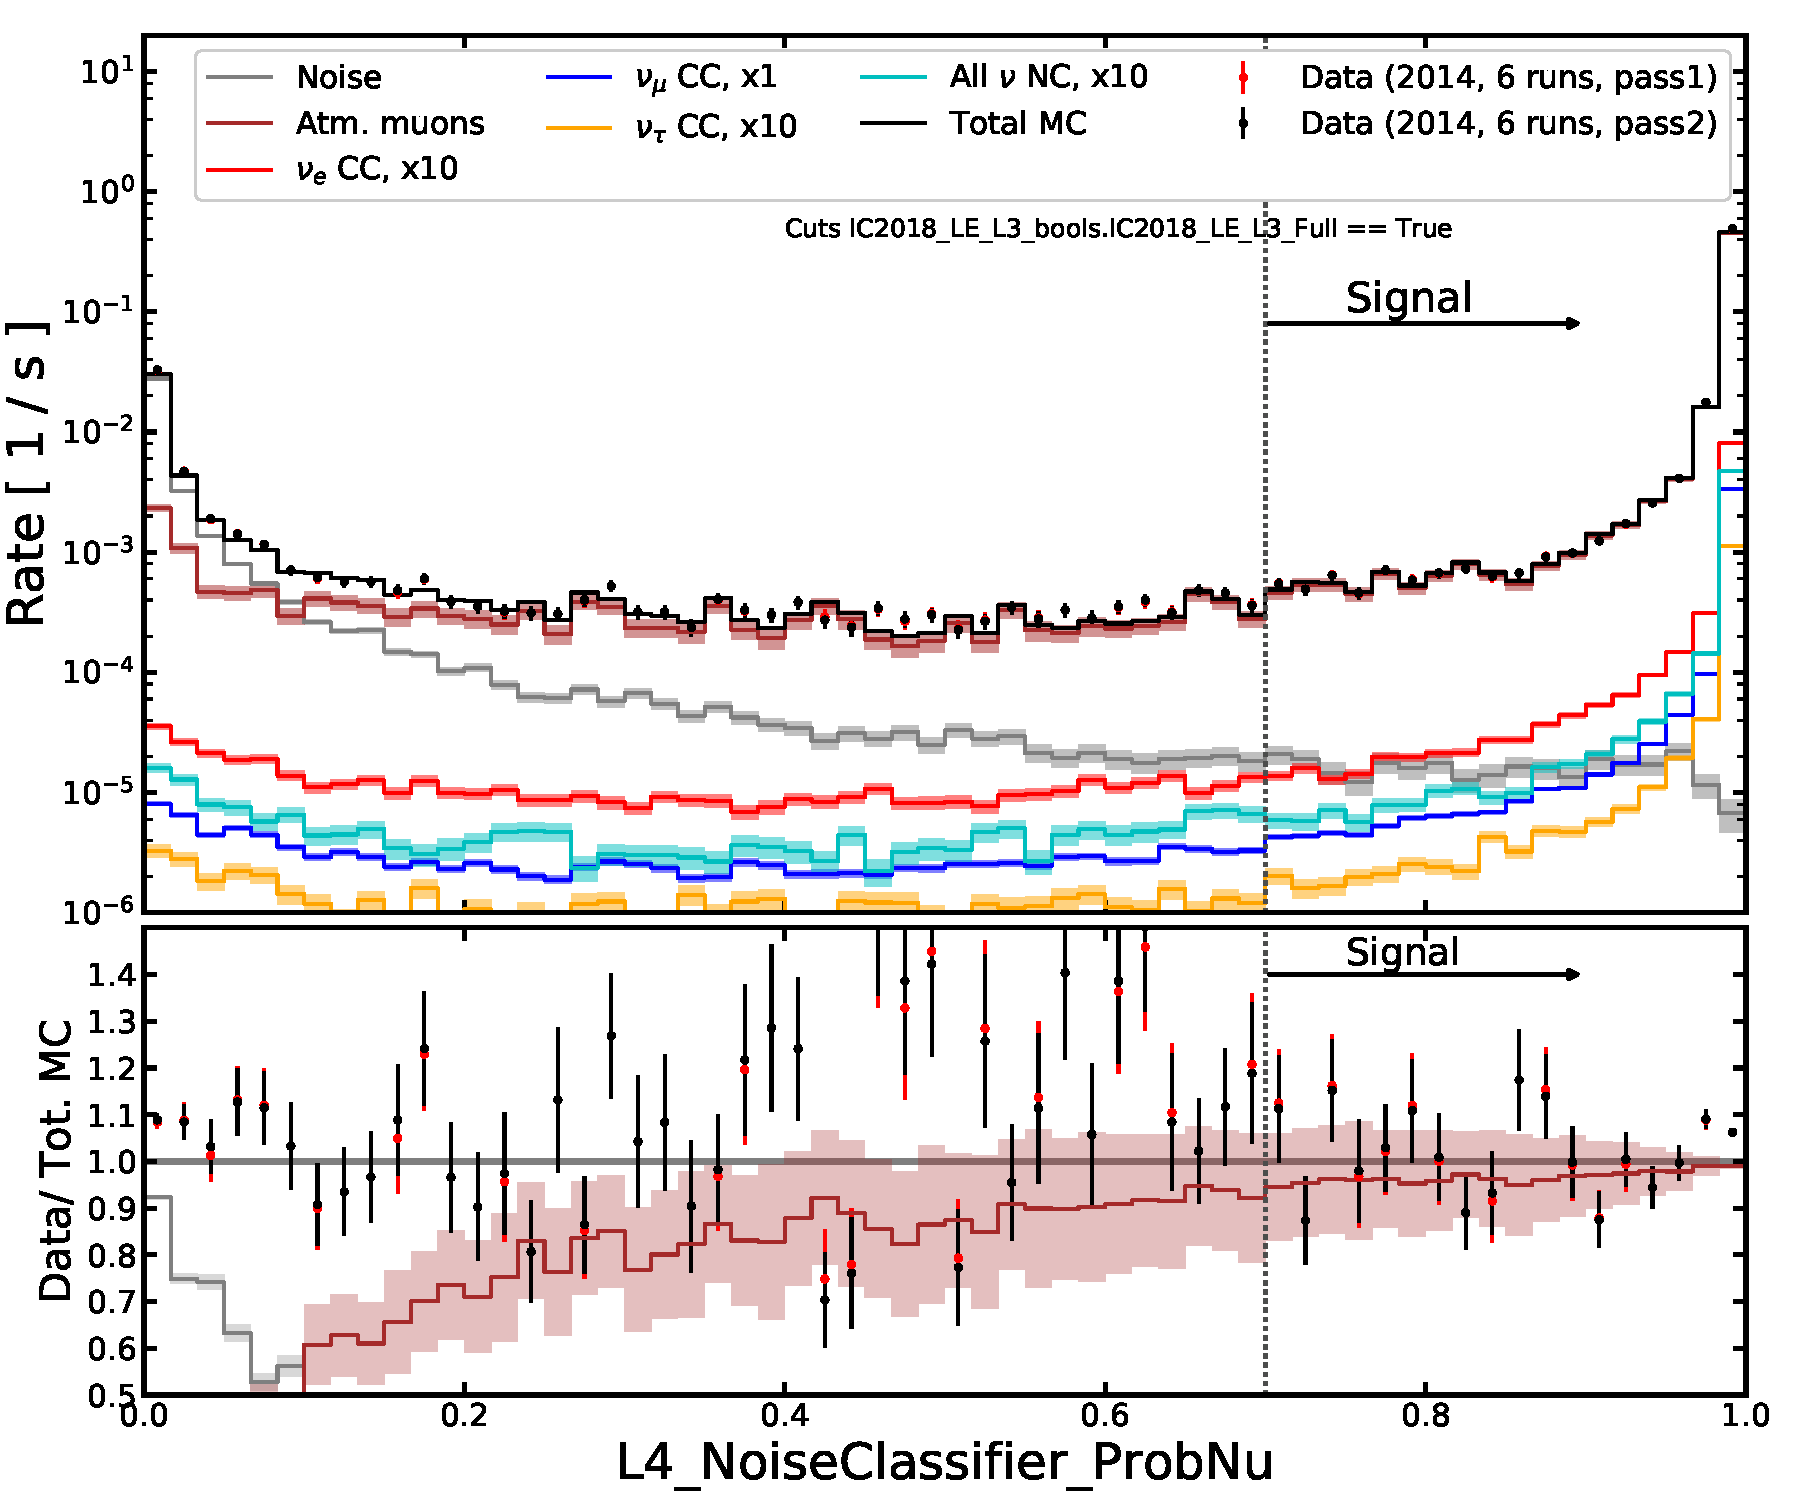
\includegraphics[width=7 cm]{figures/icecube/selection/L4_noiseBDT_L4_NoiseClassifier_ProbNu.pdf}
    %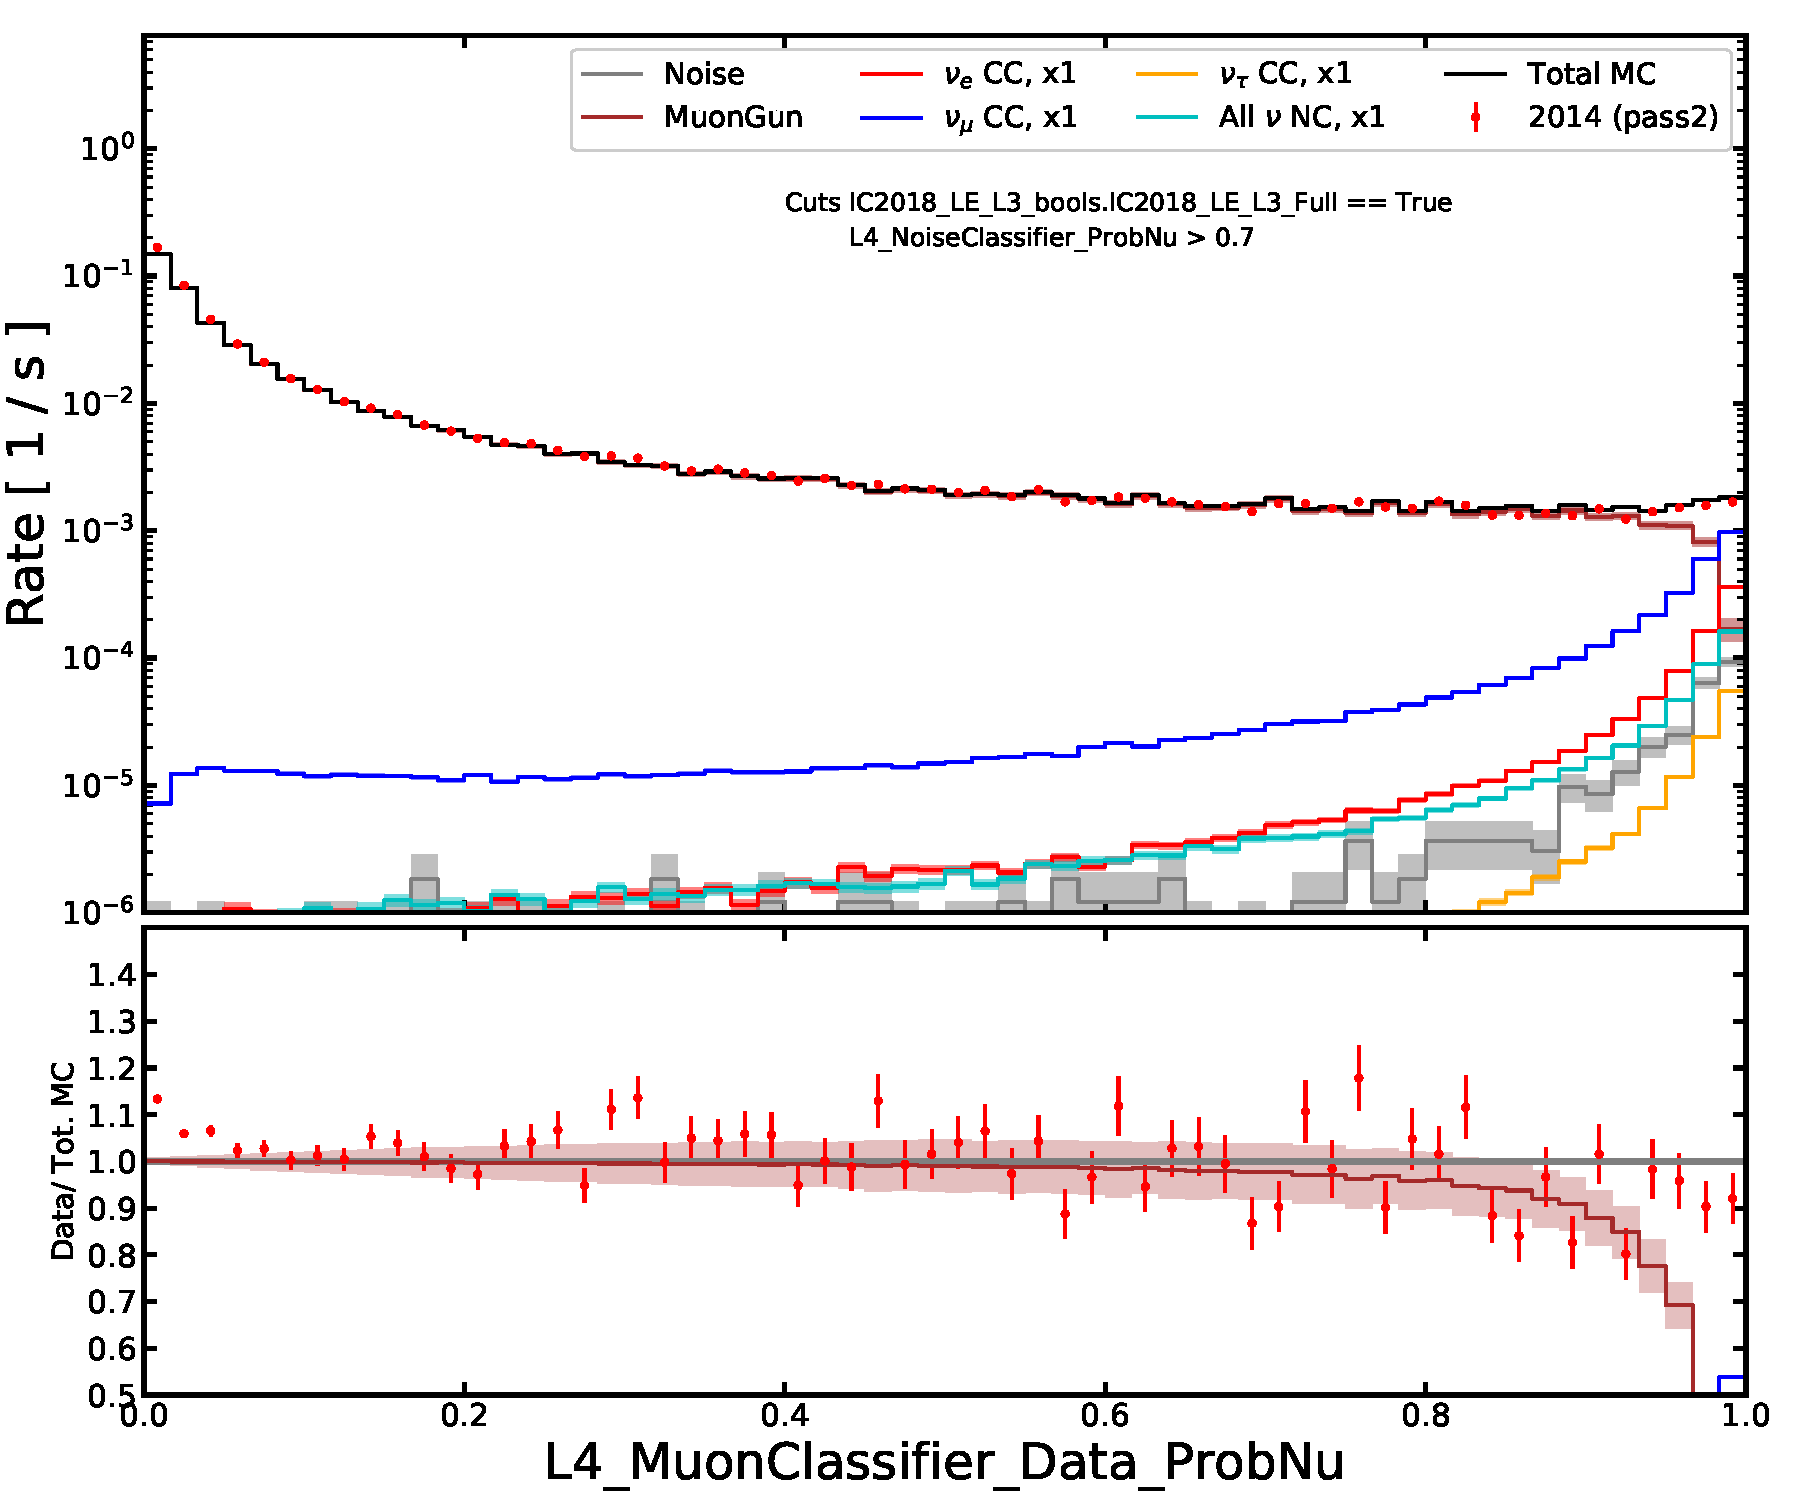
\includegraphics[width=7 cm]{figures/icecube/selection/L4_muon_L4_MuonClassifier_Data_ProbNu.pdf}
    \ref{l4_bdt_hist_legend}\hfill
    \tikzsetnextfilename{l4_noise_classifier_probnu}%
\begin{tikzpicture}
    \pgfplotstableread{figures/icecube/selection/Level4/L4_NoiseClassifier_ProbNu_level4_data_mc_hists.csv}\table
    \begin{groupplot}[
        xmin=0.0,xmax=1.0,
        xmajorgrids, ymajorgrids,
        width=0.45\linewidth,
        ylabel style={at={(-0.15,0.5)}},
        group/.cd,
        group size=1 by 2,
        xticklabels at=edge bottom,
        vertical sep=10pt,
        %every axis y label style={xshift=0.5 cm}
        ]
    \nextgroupplot[
        height=0.35\linewidth,
        legend cell align={left},
        % legend columns=-1,
        legend to name=l4_bdt_hist_legend,
        legend columns=-1,
        ymode=log,
        ymin=1e-07, ymax=1.0,
        ylabel={rate (Hz)},
        ytick distance=1e1
    ]
    \ploterrorband[muon_color]{muons}{1}
    \addlegendentry{atm. muons}
    \ploterrorband[nu_color]{nu}{1}
    \addlegendentry{atm. $\nu$}
    % \ploterrorband[nue_color]{nue}{1}
    % \addlegendentry{$\nu_e + \bar{\nu}_e$}
    % \ploterrorband[numu_color]{numu}{1}
    % \addlegendentry{$\nu_\mu + \bar{\nu}_\mu$}
    % \ploterrorband[nutau_color]{nutau}{1}
    % \addlegendentry{$\nu_\tau + \bar{\nu}_\tau$}
    \ploterrorband[noise_color]{noise}{1}
    \addlegendentry{noise}
    \ploterrorband{total_mc}{1}
    \addlegendentry{total MC}
    \ploterrorbar{data}
    \addlegendentry{season 2014
    (12 runs)}

    % draw cut
    \draw[thick,dashed] (axis cs:0.7,1e-7) -- (axis cs:0.7,10);
    \draw[-stealth, very thick] (axis cs:0.7,2e-2)  -- node[anchor=south]{\footnotesize\sffamily signal} (axis cs:0.9,2e-2);

    \nextgroupplot[
        height=0.2\linewidth,
        ymin=-0.1, ymax=1.8,
        ylabel=rate/total MC,
        xlabel={L4 NoiseClassifier ProbNu}
    ]

    \ploterrorbar{data_mc_ratio}
    \plotratioerrorband[muon_color]{muons}{total_mc}
    \plotratioerrorband[nu_color]{nu}{total_mc}
    % \plotratioerrorband[nue_color]{nue}{total_mc}
    % \plotratioerrorband[numu_color]{numu}{total_mc}
    % \plotratioerrorband[nutau_color]{nutau}{total_mc}
    \plotratioerrorband[noise_color]{noise}{total_mc}
    \end{groupplot}
\end{tikzpicture}

    \tikzsetnextfilename{l4_muon_classifier_probnu}%
\begin{tikzpicture}
    \pgfplotstableread{figures/icecube/selection/Level4/L4_MuonClassifier_Data_ProbNu_level4_data_mc_hists.csv}\table
    \begin{groupplot}[
        xmin=0.0,xmax=1.0,
        xmajorgrids, ymajorgrids,
        width=0.45\linewidth,
        ylabel style={at={(-0.15,0.5)}},
        group/.cd,
        group size=1 by 2,
        xticklabels at=edge bottom,
        vertical sep=10pt
        ]
    \nextgroupplot[
        height=0.35\linewidth,
        legend cell align={left},
        legend columns=2,
        ymode=log,
        ymin=1e-07, ymax=1.0,
        ylabel={rate (Hz)},
        ytick distance=1e1
    ]
    \ploterrorband[muon_color]{muons}{1}
    % \addlegendentry{atm. muons}
    \ploterrorband[nu_color]{nu}{1}
    % \addlegendentry{atm. $\nu$}
    % \ploterrorband[nue_color]{nue}{1}
    % % \addlegendentry{$\nu_e + \bar{\nu}_e$ x10}
    % \ploterrorband[numu_color]{numu}{1}
    % % \addlegendentry{$\nu_\mu + \bar{\nu}_\mu$ x10}
    % \ploterrorband[nutau_color]{nutau}{1}
    % % \addlegendentry{$\nu_\tau + \bar{\nu}_\tau$ x100}
    \ploterrorband[noise_color]{noise}{1}
    % \addlegendentry{noise}
    \ploterrorband{total_mc}{1}
    % \addlegendentry{total MC}

    \addplot[
        mark=*,
        mark options={scale=0.5, fill=black},
        black,
        only marks,
        error bars/.cd,
        x dir=none,
        y dir=both,
        y explicit,
    ] table [x=bin_midpoints, y=data, y error=data__err]  from \table;
    % \addlegendentry{season 2014 (12 runs)}

    % draw cut
    \draw[thick,dashed] (axis cs:0.65,1e-7) -- (axis cs:0.65,10);
    \draw[-stealth, very thick] (axis cs:0.65,2e-2)  -- node[anchor=south]{\footnotesize\sffamily signal} (axis cs:0.85,2e-2);

    \nextgroupplot[
        height=0.2\linewidth,
        ymin=-0.1, ymax=1.8,
        ylabel=rate/total MC,
        xlabel={L4 MuonClassifier Data ProbNu}
    ]

    \ploterrorbar{data_mc_ratio}
    \plotratioerrorband[muon_color]{muons}{total_mc}
    \plotratioerrorband[nu_color]{nu}{total_mc}
    % \plotratioerrorband[nue_color]{nue}{total_mc}
    % \plotratioerrorband[numu_color]{numu}{total_mc}
    % \plotratioerrorband[nutau_color]{nutau}{total_mc}
    \plotratioerrorband[noise_color]{noise}{total_mc}

    \end{groupplot}
\end{tikzpicture}


    \caption{Distribution scores for the noise (left) and muon (right) BDT. The distributions of the muon classifier are shown for events where the score of the noise BDT is greater than 0.7. Histograms show the distributions in simulated data separated by event type, data points with error bars show the distribution of real data. The bottom panel shows the ratio between data and simulation. Events falling on the "signal" side of the histogram are passed to the next filter level.}
    \label{fig:l4-bdt-output}
\end{figure*}

\subsubsection{Level 5}
The final filter that is applied before the event reconstruction step is L5.
This filter searches specifically for hits occurring in un-instrumented \emph{corridors} within the IceCube array through which an atmospheric muon can sneak into the DeepCore volume while evading previous veto cuts.
In addition, events with more than seven hits in the outermost strings of the IceCube array or that have a down-going pattern of hits in the uppermost region of the detector are vetoed to remove events containing atmospheric muons entering the detector coincidentally with neutrinos.
The distribution for one of the corridor variables and one of the muon rejection variables are shown in \reffig{l5-vars}.
Table~\ref{tab:l5_summary} shows the rates of each event type expected at each level of the selection up to L5 together with the efficiency of the filter at the final level.
\begin{figure*}
    \centering
    % 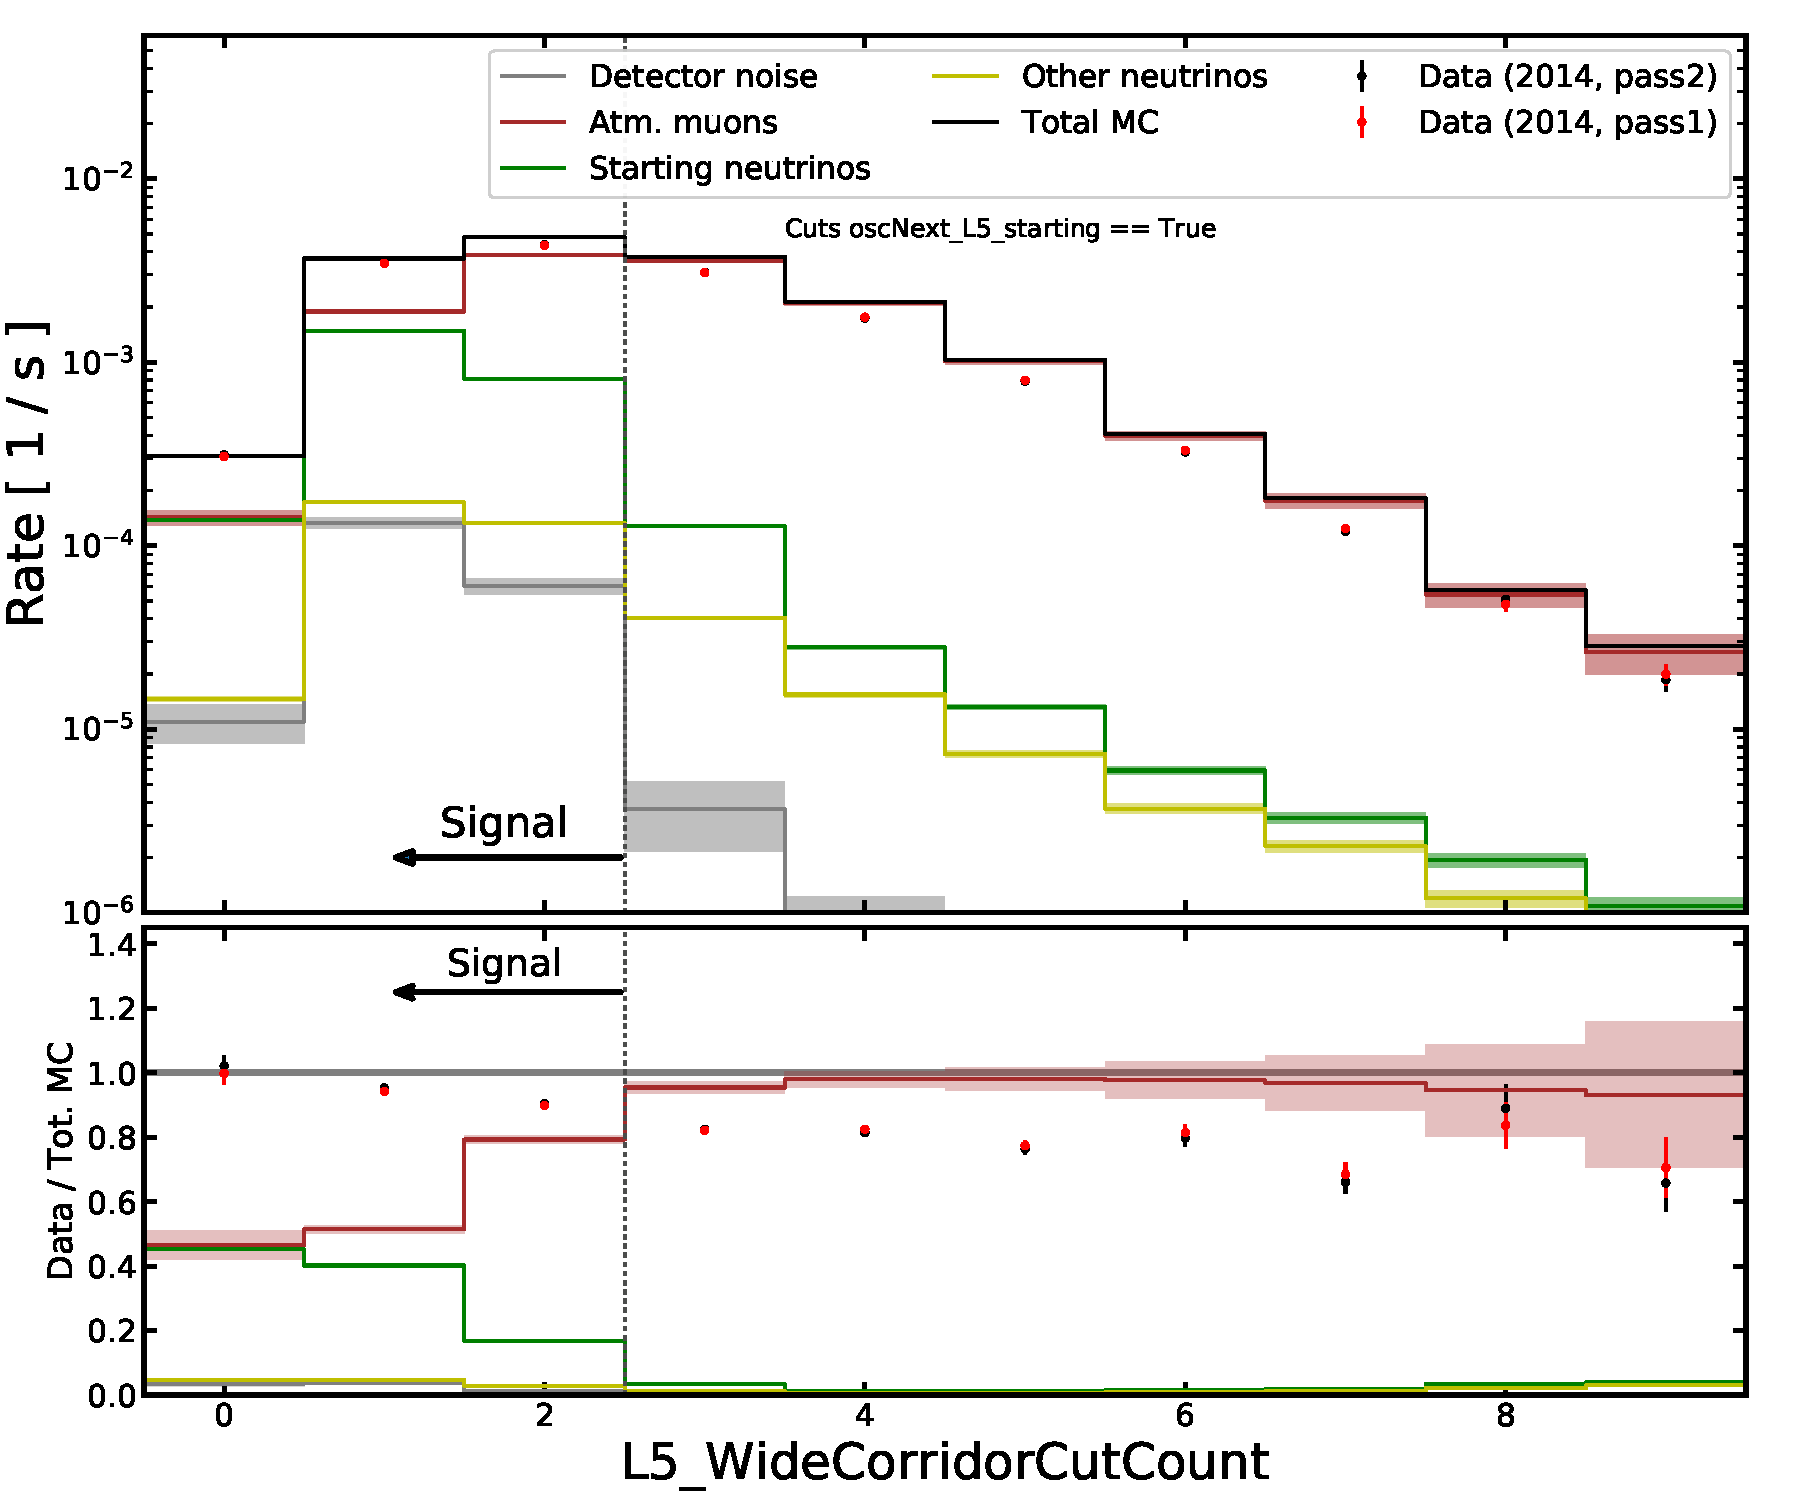
\includegraphics[width=7 cm]{figures/icecube/selection/L5_contained_L5_WideCorridorCutCount.pdf}
    % 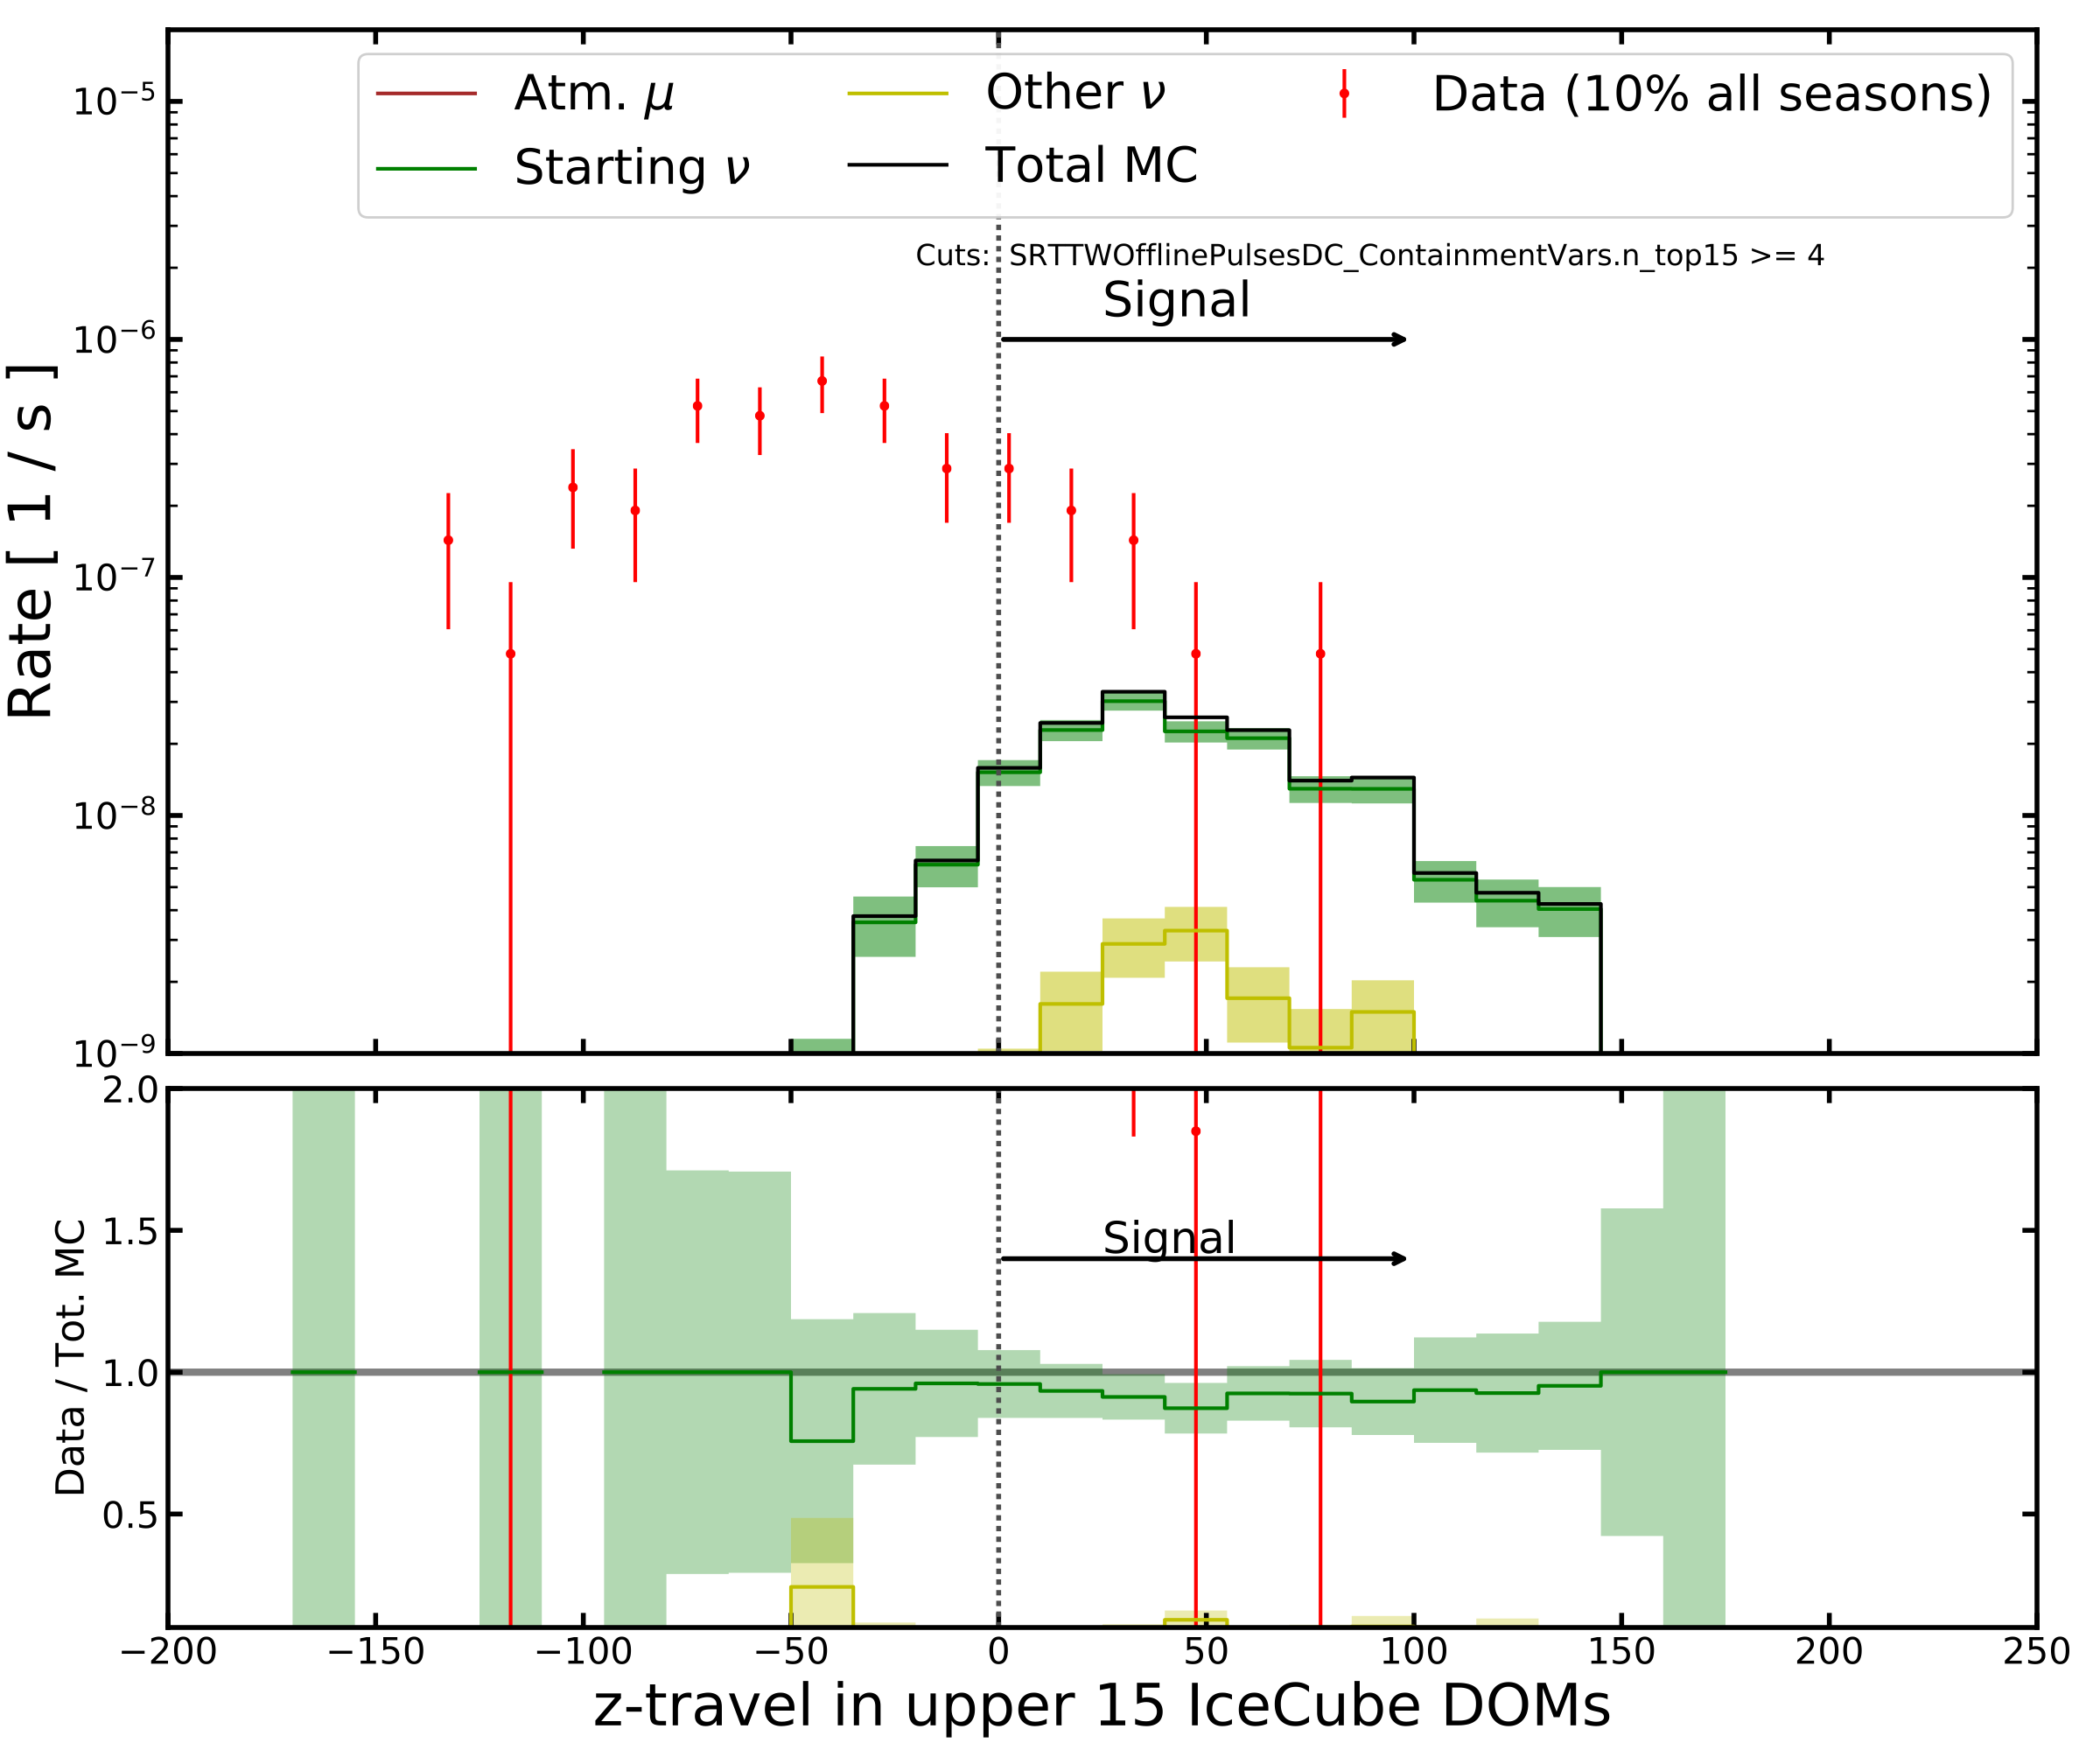
\includegraphics[width=7 cm]{figures/icecube/selection/SRTTWOfflinePulsesDC_ContainmentVars.z_travel_top15.png}
    \ref{l5_corridor_vars_legend}
    \tikzsetnextfilename{l5_corridor_cut_count}%
\begin{tikzpicture}
    \pgfplotstableread{figures/icecube/selection/Level5/L5_WideCorridorCutCount_level5_data_mc_hists.csv}\table
    \begin{groupplot}[
        xmin=0,xmax=15,
        xmajorgrids, ymajorgrids,
        width=0.45\linewidth,
        ylabel style={at={(-0.15,0.5)}},
        %scale only axis=true,
        group/.cd,
        group size=1 by 2,
        xticklabels at=edge bottom,
        vertical sep=10pt
        ]
    \nextgroupplot[
        height=0.3\linewidth,
        legend cell align={left},
        legend columns=4,
        legend to name=l5_corridor_vars_legend,
        ymode=log,
        ymin=5e-06, ymax=0.2,
        ytick distance=1e1,
        ylabel={rate (Hz)},
        y filter/.expression={y < 1e-7 ? ln(1e-8) : ln(y)}
    ]

    \ploterrorband[muon_color]{muons}{1}
    \addlegendentry{atm. muons}
    \ploterrorband[nue_color]{nue}{1}
    \addlegendentry{$\nu_e + \bar{\nu}_e$}
    \ploterrorband[numu_color]{numu}{1}
    \addlegendentry{$\nu_\mu + \bar{\nu}_\mu$}
    \ploterrorband[nutau_color]{nutau}{1}
    \addlegendentry{$\nu_\tau + \bar{\nu}_\tau$}
    \ploterrorband[noise_color]{noise}{1}
    \addlegendentry{noise}
    \ploterrorband{total_mc}{1}
    \addlegendentry{total MC}
    \addplot[
        mark=*,
        mark options={scale=0.5, fill=black},
        black,
        only marks,
        error bars/.cd,
        x dir=none,
        y dir=both,
        y explicit
    ] table [x=bin_midpoints, y=data, y error=data__err]  from \table;
    \addlegendentry{season 2014
    (12 runs)}

    % draw cut
    \draw[thick,dashed] (axis cs:2,1e-6) -- (axis cs:2,1e-1);
    \draw[stealth-, very thick] (axis cs:2,2e-2)  -- node[anchor=south]{\footnotesize\sffamily cut} (axis cs:5,2e-2);

    \nextgroupplot[
        height=0.2\linewidth,
        ymin=0, ymax=4,
        ylabel={data/MC ratio},
        xlabel={Number of hits in corridor\strut }
    ]

    \ploterrorband{data_mc_ratio}{1}
    \end{groupplot}
\end{tikzpicture}

    \tikzsetnextfilename{l5_corridor_angle_total_cos_diff}%
\begin{tikzpicture}
    \pgfplotstableread{figures/icecube/selection/Level5/L5_WideCorridorCutTrack_L5_SPEFit11_angles_total_cos_diff_level5_data_mc_hists.csv}\table
    \begin{groupplot}[
        xmin=-1.1,xmax=1.0,
        xmajorgrids, ymajorgrids,
        width=0.45\linewidth,
        ylabel style={at={(-0.15,0.5)}},
        %scale only axis=true,
        group/.cd,
        group size=1 by 2,
        xticklabels at=edge bottom,
        vertical sep=10pt
        ]
    \nextgroupplot[
        height=0.35\linewidth,
        legend cell align={left},
        legend columns=2,
        legend to name=l5_corridor_anglediff_legend,
        ymode=log,
        ymin=5e-06, ymax=2e-2,
        ytick distance=1e1,
        ylabel={rate (Hz)},
        y filter/.expression={y < 1e-7 ? ln(1e-7) : ln(y)}
    ]
    \ploterrorband[muon_color]{muons}{1}
    \addlegendentry{atm. muons}
    \ploterrorband[nue_color]{nue}{1}
    \addlegendentry{$\nu_e + \bar{\nu}_e$}
    \ploterrorband[numu_color]{numu}{1}
    \addlegendentry{$\nu_\mu + \bar{\nu}_\mu$}
    \ploterrorband[nutau_color]{nutau}{1}
    \addlegendentry{$\nu_\tau + \bar{\nu}_\tau$}
    \ploterrorband[noise_color]{noise}{1}
    \addlegendentry{noise}
    \ploterrorband{total_mc}{1}
    \addlegendentry{total MC}
    
    \addplot[
        mark=*,
        mark options={scale=0.5, fill=black},
        black,
        only marks,
        error bars/.cd,
        x dir=none,
        y dir=both,
        y explicit
    ] table [x=bin_midpoints, y=data, y error=data__err]  from \table;
    \addlegendentry{season 2014
    (12 runs)}

    % draw cut
    \draw[thick,dashed] (axis cs:0.7,1e-6) -- (axis cs:0.7,1e-2);
    \draw[-stealth, very thick] (axis cs:0.7,2e-3)  -- node[anchor=south]{\footnotesize\sffamily signal} (axis cs:0.2,2e-3);
    
    \nextgroupplot[
        height=0.2\linewidth,
        ymin=0, ymax=2,
        ylabel={data/MC ratio},
        xlabel={Cosine of angle difference to corridor\strut}
    ]
    \ploterrorband{data_mc_ratio}{1}

    \end{groupplot}
\end{tikzpicture}

    \caption{Distributions for two of the L5 corridor cut variables. Histograms show the distributions in simulated data separated by event type, data points with error bars show the distribution of real data. The bottom panel shows the ratio between data and simulation. Events falling on the "signal" side of the histogram are passed to the next filter level.}
    \label{fig:l5-vars}
\end{figure*}

\begin{table}
\caption{Summary of the rates obtained after each level of selection. Neutrinos are weighted to an atmospheric spectrum with oscillations included.}
\label{tab:l5_summary}
\begin{tabular}{lrrrrr}\toprule
& \multicolumn{4}{c}{rate ($\mu$Hz)} & \\ \cmidrule{2-5}
Event type  & DeepCore filter   & L3   & L4   & L5   & Eff. (\%) \\
\toprule
Atm. $\mu$         & 7273 & 505  & 28.1 & 0.93 & 0.012          \\
Pure noise         & 6621 & 36.6 & 0.28 & 0.07 & 0.001          \\
Atm. $\nu_e$ CC    & 1.61 & 0.95 & 0.84 & 0.48 & 29.8           \\
Atm. $\nu_\mu$ CC  & 6.16 & 3.77 & 3.11 & 1.39 & 22.5           \\
Atm. $\nu_\tau$ CC & 0.19 & 0.13 & 0.12 & 0.07 & 36.8           \\
Atm. $\nu$ NC      & 0.86 & 0.53 & 0.46 & 0.23 & 26.7  \\
\bottomrule
\end{tabular}
\end{table}

\subsection{Event Reconstruction}
\label{sec:event-reconstruction}

After the L5 selection, the rate of muons is reduced enough so that the majority of the total sample is expected to consist of atmospheric neutrinos, and it is at this point that the event reconstruction and signature classification are run.
For the measurement presented in this thesis, three reconstructed quantities are required: the zenith angle, the energy, and a proxy score determining the flavor of a neutrino.
As described in Section \ref{sec:particle-signatures}, all neutrino events in DeepCore can be effectively approximated as a cascade ($\nu_e$ CC events, all NC events and 83\% of $\nu_\tau$ CC events) or a combination of a cascade at the neutrino interaction point with an outgoing muon track ($\nu_\mu$ CC events and 17\% of $\nu_\tau$ CC events).
The zenith angle can be most accurately reconstructed for track-like events due to their elongated, highly directional signature.
For cascades, the reconstruction of the direction is more difficult because of their more compact and diffuse light distribution.
The energy of a neutrino event is reconstructed by comparing the expected light output of a combined track and cascade hypothesis with the observed hits.
Finally, the flavor proxy is calculated using variables that characterize the elongation of the observed hit signature and the goodness of fit of a combined track and cascade hypothesis compared to that of a cascade-only hypothesis.
The resulting score allows the separation of muon neutrino interactions from other interactions, which is ideally suitable to observe the muon neutrino disappearance oscillation channel.

\subsubsection{Zenith angle reconstruction}
\label{sec:santa}
The zenith angle is reconstructed using the Single-string Antares-inspired Analysis (\textsc{santa})\sidecite{Garza2014Measurement}.
It is an older algorithm aimed at reconstructing the direction of muon tracks that was originally developed for use in the ANTARES neutrino telescope~\sidecite{Aguilar:2011zz}.
It has since been refurbished and improved in IceCube, as described in detail in~\sidecite{lowen-reco-paper}.

The reconstructed pulse series in every DOM is summarized by the time of the first pulse and the sum of charges of all pulses.
This time and charge are the only information used by the reconstruction and are referred to as a \emph{hit} in the following.
The first step of the reconstruction algorithm is a cleaning routine that removes hits produced
by photons that have been scattered many times as they traveled
through the ice, leaving only hits from photons that have traveled in approximately straight lines based on the time difference between hits on the same string.
%The algorithm is a simplification from an earlier implementation described in \cite{Garza2014Measurement}.
It calculates the signal speed between hits on the same string, and removes a hit if this velocity is below the speed of light in ice.
This is a simplification of the algorithm described in \cite{Garza2014Measurement}, where the effective signal velocity was updated during the selection process.
The selection is run separately for each string, and if fewer than three hits remain on a string, all hits on the string are discarded.
In total, it is necessary for at least five hits to remain in an event in order to run the directional reconstruction.
If only hits on one string remain after the selection, the event is referred to as a \emph{single-string} event, otherwise it is a \emph{multi-string} event.
The reconstruction is generally more accurate for multi-string events, because the spacing between strings provides a long lever arm to constrain the direction of a track.
In addition, the azimuth angle of the track can only be reconstructed for \emph{multi-string} events due to the rotational symmetry of a single string.

\begin{figure*}
    \centering
    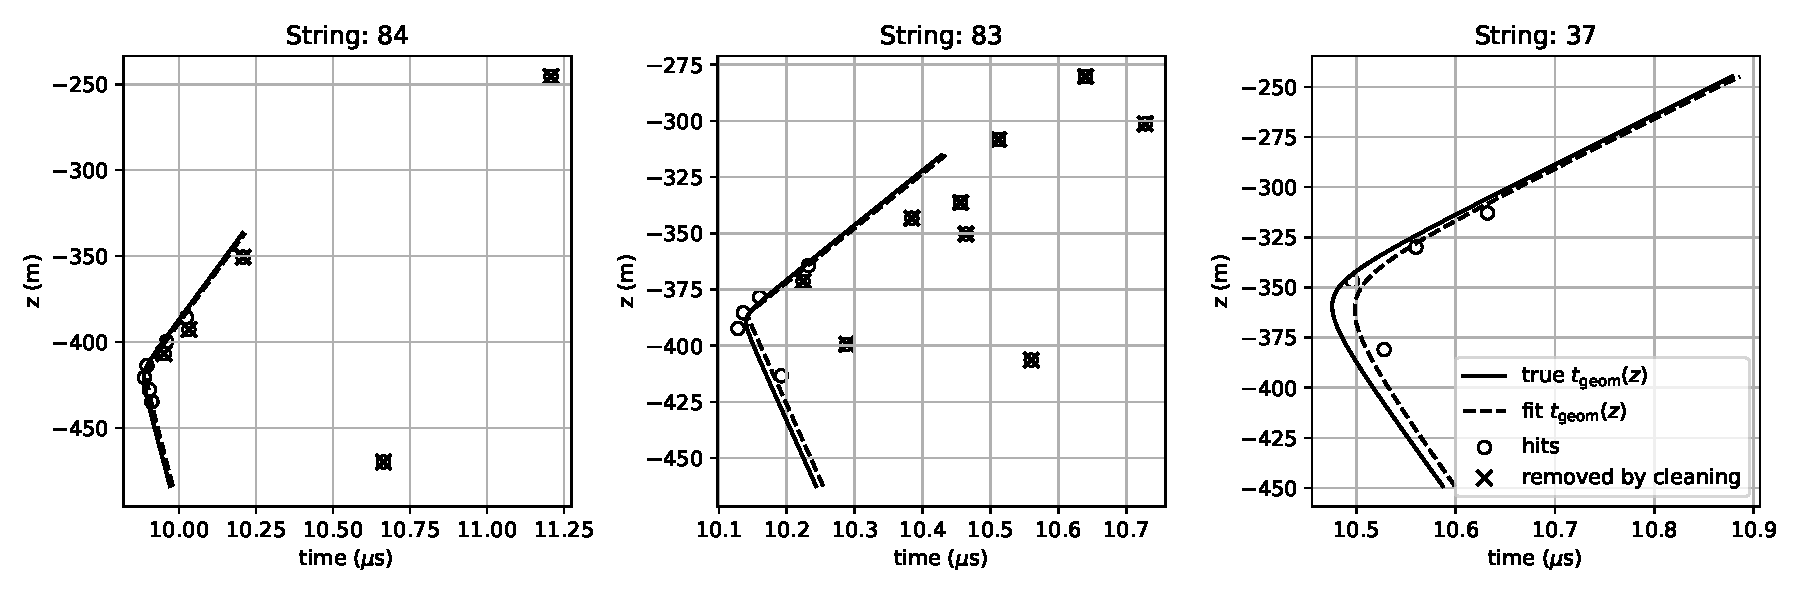
\includegraphics[width=\linewidth]{figures/icecube/reconstruction/santa/multi_string_example_with_cleaning_id_12607962.pdf}
    \caption{Example of a \numucc event reconstructed with \textsc{santa} with hits on several strings. Strings 84, 83 and 37 are spaced $\sim80\,\mathrm{m}$ apart from each other and form a highly obtuse triangle.}
    \label{fig:santa-multi-string-example}
\end{figure*}

The directional reconstruction itself is a regression that minimizes a modified $\chi^2$ loss that is defined as
\begin{equation}
L(\vec{\theta})=\sum_{i=1}^{N}\phi(r^2_i(\vec{\theta}))
+
\frac{1}{\bar{q}}\sum_{i=1}^{N}\tilde{q}_i \frac{d_{\gamma,i}}{d_0}\,.\label{eq:chi-square-mod-loss}
\end{equation}
The first term in \refeq{chi-square-mod-loss} is a $\chi^2$ loss that is modified to be robust against outliers. The second term is a regularization term that penalizes solutions where large charges are observed at large distances. Here, $r^2_i$ is the chi-square residual for each observed hit, $i$, between the observed time, $t_{\mathrm{obs}, i}$ and the geometric arrival time, $t_{\mathrm{geom},i}(\vec{\theta})$,
\begin{equation}
r_{i}^{2}(\vec{\theta})=\left(\frac{t_{\mathrm{geom},i}(\vec{\theta})-t_{\mathrm{obs},i}}{\sigma_{t}}\right)^{2}\,.
\end{equation}
The residual is wrapped in a \emph{robust loss function}, $\phi(r_{i}^{2})=\log\left(1+r_{i}^{2}/C^2\right)C^2$, which grows much more slowly than $r_{i}^{2}$ for values of $r_i$ greater than the "soft cutoff", $C$, while behaves very similarly to $r_i^2$ for values of $r_i$ smaller than $C$.
Effectively, this robust loss reduces the influence of hits that pass the hit selection procedure despite having undergone a significant amount of scattering.
The uncertainty in the pulse-time measurement is approximately $\sigma_{t}=3\,\mathrm{ns}$, corresponding to the readout rate of the modules~\cite{icecube_daq}.

In the second term of \refeq{chi-square-mod-loss}, $\tilde{q}_i$ is the total observed charge in DOM $i$ divided by the effective area of the DOM at the angle of incidence of the photon, and $\bar{q}$ is the average over all $\tilde{q}_i$.
For every DOM, the charge per effective area is multiplied by the distance traveled by the photon, $d_{\gamma,i}$, and divided by a typical scaling distance, $d_0$.
The distance $d_0$ determines the strength of the regularization term and has been optimized empirically to achieve the optimal resolution of the reconstruction to a value of \SI{7}{\meter}.

The expected arrival time for unscattered Cherenkov photons is calculated geometrically under the assumption of an infinitely long track characterized by a normalized direction vector $\vec{u}=(u_{x},u_{y},u_{z})$,
an anchor point $\vec{q}=(q_{x},q_{y},q_{z})$ and a time $t_{0}$
at which the particle passes through $\vec{q}$.
The
velocity is fixed to the vacuum speed of light, $c$.
Since the reconstruction ignores DOMs that have not recorded any pulses, the fact that the true track length is finite only makes a negligible  difference.
The arrangement of these vectors is shown in \reffig{Detailed-track-geometry}.
Without scattering, all Cherenkov photons lie on a cone with an opening
angle $\theta_{c}$
\begin{figure}[h]
\begin{centering}
\tikzsetnextfilename{track_geometry_santa}%
\begin{tikzpicture}[scale=1,>=stealth]
	\path[name path=track] (0,3) -- (9,3);
	\node[shape=star,
	      star point height=1cm,
	      star point ratio=0.5,
	      draw, fill=black,
	      label=below:$\vec{p}(t_{\mathrm{em}})$] (emission) at (1,3) {};
	\draw[->, decorate,
	decoration={snake,amplitude=.4mm,segment length=2mm,post length=1mm}]
		(emission.center)
		-- node[sloped, above] {$d_{\gamma}$} +(40:4)
		node[label=above:DOM at $\vec{r}$] (dompos) {};
	\path[name path=cone] (dompos.center) -- +(-50:4);
	\draw[name intersections={of=track and cone, by=tip}]
		(dompos.center) -- node[sloped, above] {Cherenkov light cone} (tip)
		node[label=below:$\vec{p}(t_{\mathrm{geom}})$] (muonpos) {};
	\draw[fill=black, opacity=0.5] (dompos.center) circle (5pt);
	\draw[color=black, ->, style=very thick] (0,3) node[anchor=north]{muon} -- (muonpos.center);
	\draw (emission.center) +(1,0) node[anchor=south east]{$\theta_c$}  arc (0:40:1);
	\path (emission.center)
		-- node[shape=circle,
			fill=black,
			label=below:$\vec{q}$] (vertex) {}
		(tip);
	\draw[->] (vertex.center) -- node[sloped, below] {$\vec{r}-\vec{q}$} (dompos.center);
	%\draw (vertex.center) +(-1,0) arc (180:140:1);
	%\path (vertex.center) -- +(160:0.6) node {$\theta$};
	\draw[->] (vertex.center) ++(0.2, 0.2) -- node[above] {$\vec{u}$} +(1,0);
\end{tikzpicture}\par
\end{centering}
\caption{\label{fig:Detailed-track-geometry}Detailed geometry of a light cone
created by a track.
$\vec{q}$ is the position of the anchor point
and $\vec{r}$ is the position of the optical module. $\vec{p}(t_{\mathrm{em}})$
and $\vec{p}(t_{\mathrm{geom}})$ are the positions of the muon at
the time the photon is emitted and when it is geometrically expected
to arrive, respectively.}
\end{figure}
whose tip is in the position of the particle at the time $\vec{p}(t)$. The opening angle satisfies $\cos(\theta_c)=1/n_{\mathrm{ph}}$, where $n_{\mathrm{ph}}$ is the phase index of refraction of the ice.
Assuming that a photon has traveled in a straight line at the group velocity in ice, the geometric arrival time, $t_{\mathrm{geom}}$, for a DOM at position $\vec{r}$ is

\begin{equation}
t_{\mathrm{geom}}=t_{0}+\frac{1}{c}\left(\left(\vec{r}-\vec{q}\right)\cdot\vec{u}+\frac{d_{\gamma}}{n_{\mathrm{ph}}}\left(n_{\mathrm{ph}}n_{\mathrm{gr}}-1\right)\right)\label{eq:t_geom-MS-track}
\end{equation}
where the distance traveled by the photon $d_\gamma$ is
\begin{equation}
d_{\gamma}=n_{\mathrm{ph}}\sqrt{\frac{1}{n_{\mathrm{ph}}^{2}-1}\left(\vec{u}\times\left(\vec{r}-\vec{q}\right)\right)^{2}}\,.\label{eq:photon-distance-3d}
\end{equation}

\begin{figure}
    \centering
    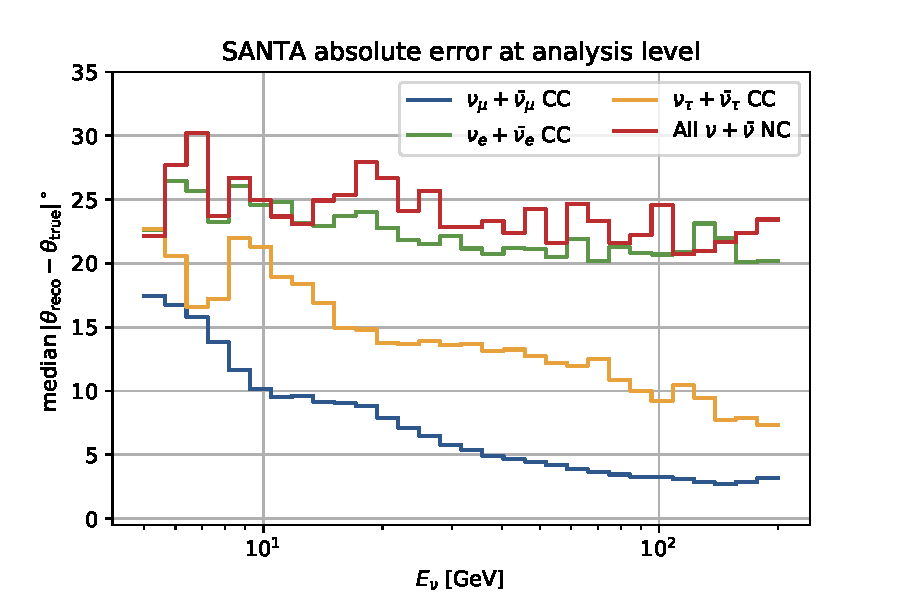
\includegraphics[width=0.8\linewidth]{figures/icecube/reconstruction/santa/santa_absolute_error_final.pdf}
    \caption{Median error on the reconstructed zenith angle at the final level of the sample selection as a function of the true simulated neutrino energy.}
    \label{fig:santa-resolution}
\end{figure}

The group and phase indices of refraction depend on the wavelength, but for this reconstruction the value for a wavelength of $\lambda=400\;\mathrm{nm}$
\footnote{$400\;\mathrm{nm}$ is near the wavelength of the highest acceptance of the optical modules.\cite{icecube_detector_17}} is used, where $n_{\mathrm{gr}}=1.356$ and $n_{\mathrm{ph}}=1.319$~from~\sidecite{PRICE200197}.
An example of a simulated event reconstructed with \textsc{santa} is shown in \reffig{santa-multi-string-example}.
The solid and dashed lines show the geometric arrival time calculated according to equation~\ref{eq:t_geom-MS-track} using reconstructed and true track parameters, respectively.
The circles indicate hits in DOMs, and those hits that have been removed by the hit cleaning procedure are crossed out.
The median error on the zenith angle reconstructed using \textsc{SANTA} is shown in \reffig{santa-resolution}, split by neutrino interaction type.
As expected, the error is the smallest for $\nu_\mu$-CC interactions, since those produce track signatures that most closely resemble the infinite track hypothesis underlying the \textsc{SANTA} reconstruction algorithm.
The worst resolution is achieved for interactions that only produce electronic or hadronic showers, since they produce cascade signatures hardly resembling the infinite track assumption.
It is also apparent that the median resolution for $\nu_\tau$-CC events lies between that of $\nu_\mu$-CC events and pure cascade events.
This is readily explained by the fact that 17\% of these interactions also produce a muon in their final state.

In addition to the zenith angle reconstruction, SANTA can also be used to fit a simplified cascade hypothesis to the observed hits.
For this purpose, it is assumed that light is emitted uniformly in all directions originating from the interaction vertex as shown in the left panel in \reffig{idealized_signatures}.
With this assumption of perfect rotational symmetry, it is not possible to reconstruct a direction, and the cascade is fully characterized by the position of the vertex and the interaction time.
The ratio of the $\chi^2$ of the infinite-track regression and the $\chi^2$ of this \emph{cascade-only} regression is used as a proxy for the neutrino flavor in this analysis.
If it is smaller than one, the infinite-track hypothesis achieves a better fit to the data than the cascade-only hypothesis.

\subsubsection{Energy reconstruction}
\label{sec:leera}
The energy reconstruction runs as a separate step after the zenith angle reconstruction.
In contrast to \textsc{SANTA}, the Low-Energy Energy Reconstruction Algorithm (LEERA)\cite{Terliuk2018Measurement} fits a combined hypothesis consisting of a cascade and a finite-length track originating at the same point of the cascade.
Both the cascade and the track are constrained to move only along the infinite track that has been fit in the zenith reconstruction.
This means that the model fit in the energy reconstruction is fully characterized by the shift of the vertex along the infinite track, the length of the finite track (which is linearly related to the track energy), and the energy of the cascade.
Given these parameters, the expected light yield for all DOMs is calculated using the so-called \emph{photonics tables}.
The tables consist of B-spline coefficients that have been fit to simulated photon propagation for cascades and 3~m long tracks segments at different depths and directions inside the IceCube array to give a (time-dependent) expectation value for the photon count at arbitrary positions inside the detector.
The expectation of an arbitrarily long track is calculated by chaining the 3~m segments together that fully cover the desired track length, and scaling the amplitude of the last segment by the remainder of the division of the desired length by the length of the segments.
Given these expectation values as a function of event parameters, $\lambda_i(\theta)$, for every DOM, $i$, a simple Poisson ''hit vs.
no-hit'' log-likelihood is calculated as
\begin{equation}
    \log(\mathcal{L}) = \sum_{i\in\mathrm{DOMs\;without\;hits}} e^{-\lambda_i(\theta)} + \sum_{i\in\mathrm{DOMs\;with\;hits}} (1 - e^{-\lambda_i(\theta)})\;.
    \label{eq:leera-llh}
\end{equation}
This likelihood is maximized under the hypothesis that the shift, track length, and cascade energy are all free parameters, and under the alternative hypothesis where the track length is fixed to zero, the latter of which corresponds to a cascade-only hypothesis. The difference between these two log-likelihoods provides a measure of the degree to which the combined track and cascade hypothesis fits the observed data better than a track-only hypothesis. It is one of the inputs that is used in a BDT to calculate an overall score of how track-like an observed event signature is. The median relative error in the reconstructed total energy (that is, the sum of the track energy and the cascade energy) is shown in \reffig{leera-resolution}. As with the zenith angle reconstruction, the relative error is smallest for \numucc-events. This is expected, since these events fit the hypothesis of an initial cascade combined with a finite track the best. The second-best resolution is achieved for $\nu_{e,\mathrm{CC}}$-events, while it is poorest for $\nu_{\tau,\mathrm{CC}}$ and neutral-current events. This is explained by the fact that the expected light yield that is put in Equation~\ref{eq:leera-llh} is based on the assumption that all particles that are produced in the interaction are visible to the detector. While this assumption is a good approximation for $\nu_{e,\mathrm{CC}}$-events, it does not hold for hadronic cascades that contain some neutral components as discussed in chapter~\ref{sec:had-showers}.
The true energy of the primary particles that produce hadronic cascades is therefore systematically under-estimated and has a larger uncertainty.
This additional uncertainty is fundamentally irreducible, because it is not possible to distinguish the signatures of hadronic and electromagnetic showers.

\begin{figure}
    \centering
    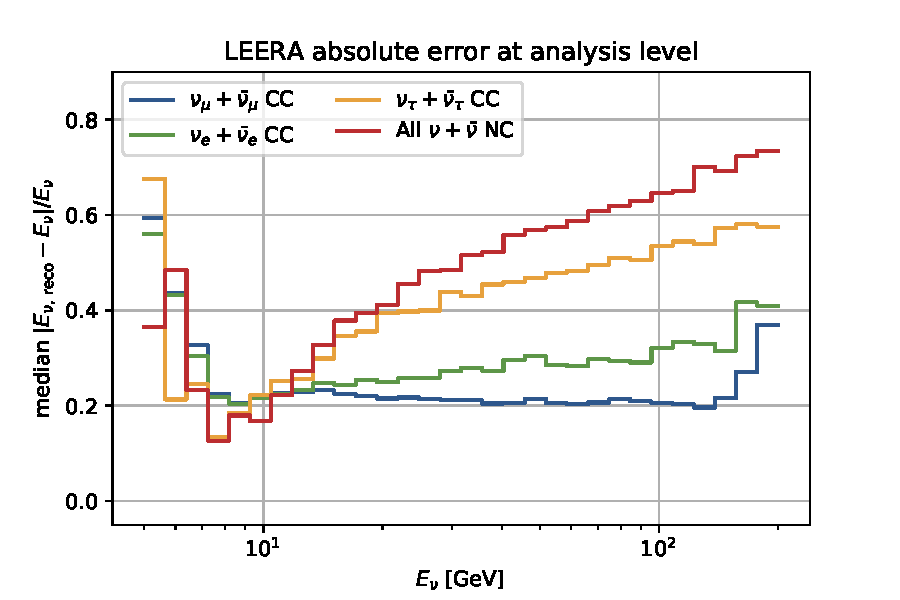
\includegraphics[width=0.8\linewidth]{figures/icecube/reconstruction/leera/leera_absolute_error_final.pdf}
    \caption{Median fractional error on the reconstructed energy at the final level of the sample selection as a function of neutrino energy.}
    \label{fig:leera-resolution}
\end{figure}

\subsection{Signature Classification}
\label{sec:pid}
In addition to the energy and zenith angle, the measurement presented in this thesis requires a score that separates track-like \numucc-events from other types of interaction.
While previous analyses used only single variables such as the reconstructed track length to differentiate between tracks and cascades~\cite{deepcore_sterile_2017, Aartsen_2015,IceCube:2019dqi}, the analysis presented in this thesis uses several variables as input into a Boosted Decision-Tree (BDT) to compute a score for how track-like the observed signature is.
The BDT classifier is taken from the \texttt{scikit-learn}\cite{scikit-learn} package and trained to classify between tracks and cascades using the following input variables:
\begin{itemize}
    \item SANTA $\chi^2\textrm{-ratio}$, defined as  $\frac{(\chi^{2}/\mathrm{d.o.f.})_{\mathrm{track}}}{(\chi^{2}/\mathrm{d.o.f.})_{\mathrm{cascade}}}$, i.e.
the ratio of goodness-of-fit metrics from each fit hypothesis in the directional reconstruction (see section \ref{sec:santa})
    \item $\Delta$LLH from energy reconstruction, defined as LLH$_\mathrm{track}-$LLH$_\mathrm{cascade}$, i.e.
the best-fit LLH value from each hypothesis
    \item Reconstructed muon track length, $L_{\mu}$
    \item Radial distance of the reconstructed interaction vertex from string 36\footnote{String 36 is approximately at the center of the array, and near to the densest region of DeepCore (see \reffig{icecube-schematic}).}, $\rho^{36}_{vertex}$
    \item Radial distance of the end-point from string 36, $\rho^{36}_{stop}$
    \item Depth of the interaction vertex, $z_{vertex}$
    \item Depth of the end point, $z_{stop}$
\end{itemize}
\begin{figure*}
    \centering
    \ref{leera_pid_legend}


    \tikzsetnextfilename{santa_pid_prefit}%
\begin{tikzpicture}
    \pgfplotstableread{figures/icecube/classification/variables/SANTA_PID.csv}\table
    \begin{groupplot}[
        xmin=-0.25,xmax=5.25,
        xmode=normal,
        xmajorgrids, ymajorgrids,
        width=0.45\linewidth,
        ylabel style={at={(-0.15,0.5)}},
        group/.cd,
        group size=1 by 2,
        xticklabels at=edge bottom,
        vertical sep=10pt
        ]
    \nextgroupplot[
        height=0.35\linewidth,
        legend cell align={left},
        legend columns=4,
        legend to name=santa_pid_legend,
        ymode=log,
        ymin=5.937489735229232e-11, ymax=0.05052335190265824,
        ylabel=rate (Hz),
        % add magic filter to correctly handle empty bins in logarithmic y-axes:
        % If a bin-count is too low or zero, it would cause the line to be
        % interrupted, which creates artefacts and ugliness. Instead, we replace
        % these bin-counts with values that are just below the axis limit.
        % Because of the way pgfplots works, the input is the raw number but the
        % output has to be the log. Weird, I know.
        y filter/.expression={y < 5.937489735229232e-11 ? ln(5.937489735229232e-12) : ln(y)}
    ]

    % \ploterrorband[muon_color]{muon}{1}
    % \addlegendentry{atm. muons}

    % \ploterrorband[nue_color]{nuenuebar}{1}
    % \addlegendentry{$\nu_e + \bar{\nu}_e$}

    % \ploterrorband[numu_color]{numunumubar}{1}
    % \addlegendentry{$\nu_\mu + \bar{\nu}_\mu$}

    % \ploterrorband[nutau_color]{nutaunutaubar}{1}
    % \addlegendentry{$\nu_\tau + \bar{\nu}_\tau$}


    % alternative event breakdown by interaction
    \ploterrorband[nue_color]{nue_ccnuebar_cc}{1}
    \addlegendentry{$\nu_e + \bar{\nu}_e$, CC}
    
    \ploterrorband[numu_color]{numu_ccnumubar_cc}{1}
    \addlegendentry{$\nu_\mu + \bar{\nu}_\mu$, CC}
    
    \ploterrorband[nutau_color]{nutau_ccnutaubar_cc}{1}
    \addlegendentry{$\nu_\tau + \bar{\nu}_\tau$, CC}
    
    \ploterrorband[nc_color]{nuall_ncnuallbar_nc}{1}
    \addlegendentry{all $\nu$, NC}

    \ploterrorband{total_mc}{1}
    \addlegendentry{total MC}

    \addplot[
        mark=*,
        mark options={scale=0.5, fill=black},
        black,
        only marks,
        error bars/.cd,
        x dir=none,
        y dir=both,
        y explicit
    ] table [x=bin_midpoints, y=data, y error=data__err]  from \table;
    \addlegendentry{data}


    \nextgroupplot[
        height=0.2\linewidth,
        ymin=0.5, ymax=1.5,
        ylabel=data/MC ratio,
        xlabel=SANTA $\chi^2\textrm{-ratio}$
    ]

    \ploterrorband{data_mc_ratio}{1}
    % \ploterrorband[numu_color]{numu_ccnumubar_cc_frac}{1}
    \end{groupplot}
\end{tikzpicture}

    \tikzsetnextfilename{leera_pid_prefit}%
\begin{tikzpicture}
    \pgfplotstableread{figures/icecube/classification/variables/LEERA_PID.csv}\table
    \begin{groupplot}[
        xmin=-22.0,xmax=22.0,
        xmode=normal,
        xmajorgrids, ymajorgrids,
        width=0.45\linewidth,
        ylabel style={at={(-0.15,0.5)}},
        group/.cd,
        group size=1 by 2,
        xticklabels at=edge bottom,
        vertical sep=10pt
        ]
    \nextgroupplot[
        height=0.35\linewidth,
        legend cell align={left},
        legend columns=4,
        legend to name=leera_pid_legend,
        ymode=log,
        ymin=4.429678646618006e-09, ymax=5e-3,
        ylabel=rate (Hz),
        % add magic filter to correctly handle empty bins in logarithmic y-axes:
        % If a bin-count is too low or zero, it would cause the line to be
        % interrupted, which creates artefacts and ugliness. Instead, we replace
        % these bin-counts with values that are just below the axis limit.
        % Because of the way pgfplots works, the input is the raw number but the
        % output has to be the log. Weird, I know.
        y filter/.expression={y < 4.429678646618006e-09 ? ln(4.429678646618006e-10) : ln(y)}
    ]

    % \ploterrorband[muon_color]{muon}{1}
    % \addlegendentry{atm. muons}

    % \ploterrorband[nue_color]{nuenuebar}{1}
    % \addlegendentry{$\nu_e + \bar{\nu}_e$}

    % \ploterrorband[numu_color]{numunumubar}{1}
    % \addlegendentry{$\nu_\mu + \bar{\nu}_\mu$}

    % \ploterrorband[nutau_color]{nutaunutaubar}{1}
    % \addlegendentry{$\nu_\tau + \bar{\nu}_\tau$}


    % alternative event breakdown by interaction
    \ploterrorband[nue_color]{nue_ccnuebar_cc}{1}
    \addlegendentry{$\nu_e + \bar{\nu}_e$, CC}
    
    \ploterrorband[numu_color]{numu_ccnumubar_cc}{1}
    \addlegendentry{$\nu_\mu + \bar{\nu}_\mu$, CC}
    
    \ploterrorband[nutau_color]{nutau_ccnutaubar_cc}{1}
    \addlegendentry{$\nu_\tau + \bar{\nu}_\tau$, CC}
    
    \ploterrorband[nc_color]{nuall_ncnuallbar_nc}{1}
    \addlegendentry{all $\nu$, NC}

    \ploterrorband{total_mc}{1}
    \addlegendentry{total MC}

    \addplot[
        mark=*,
        mark options={scale=0.5, fill=black},
        black,
        only marks,
        error bars/.cd,
        x dir=none,
        y dir=both,
        y explicit
    ] table [x=bin_midpoints, y=data, y error=data__err]  from \table;
    \addlegendentry{data}


    \nextgroupplot[
        height=0.2\linewidth,
        ymin=0.5, ymax=1.5,
        ylabel=data/MC ratio,
        xlabel=LLH$_\mathrm{track}-$LLH$_\mathrm{cascade}$
    ]

    \ploterrorband{data_mc_ratio}{1}
    % \ploterrorband[numu_color]{numu_ccnumubar_cc_frac}{1}
    \end{groupplot}
\end{tikzpicture}

    \caption{Distribution and data/MC comparison for the two most important input variables into the classification BDT.}
    \label{fig:bdt-input-vars}
\end{figure*}
Of these variables, the SANTA $\chi^2\textrm{-ratio}$ and $\Delta$LLH contribute the most to the final score.
Their distributions and comparison between data and simulation can be seen in \reffig{bdt-input-vars} at the L5 selection level, where neutrinos are weighted with \textsc{NuFit}~4.0\cite{nufit40} global fit parameters.
The training data consists of simulated $\nu_e$-CC interactions and neutral-current interactions representing cascades, and $\nu_\mu$-CC interactions representing tracks.
Tau neutrino interactions are not included in the training data in order to avoid confusion due to the 17\% of $\nu_\tau$-CC interactions that produce track-like signatures.
The training samples are weighted to approximate the neutrino flux expected from the HKKM model~\sidecite{Honda:2015fha} \emph{without} oscillations.
The distributions for these variables for tracks and cascades as they were used in training can be found in the Appendix~\ref{sec:apx-pidvars}.
To guard against over-training of the classifier, only half of the available simulation is used for training, while the other half is held out for validation.
The output score of the classifier is referred to as \emph{particle-ID} (PID) and ranges from zero (very cascade-like) to one (very track-like).
The distribution of the PID score for simulated neutrino interactions is shown in \reffig{pid-score}, broken down by flavor and interaction type.
The distributions are individually normalized to help visualize the shape differences between the different neutrino interactions.
The distributions for all interaction types show a large peak around a probability score of 0.5, suggesting that the event signature cannot be clearly classified for the majority of events.
A second peak exists only in the distribution of $\nu_\mu$-CC events close to a score of one, meaning that there exists a population of these events that can be very clearly classified as being track-like.
There also exists some excess of high PID values in the distribution of $\nu_\tau$-CC events corresponding to those events where the decay of the tauon produces a muon.
Notably, there is no population of events that can be cleanly classified as a cascade event, i.e., there are no PID scores close to zero.
The reason for this is that the two classes are nested hypotheses, one containing only a cascade and the other containing a combination of a cascade and a track, and it is never possible to prove that a cascade-like signature does not contain at least a short track segment.
\begin{figure}
    \centering
    %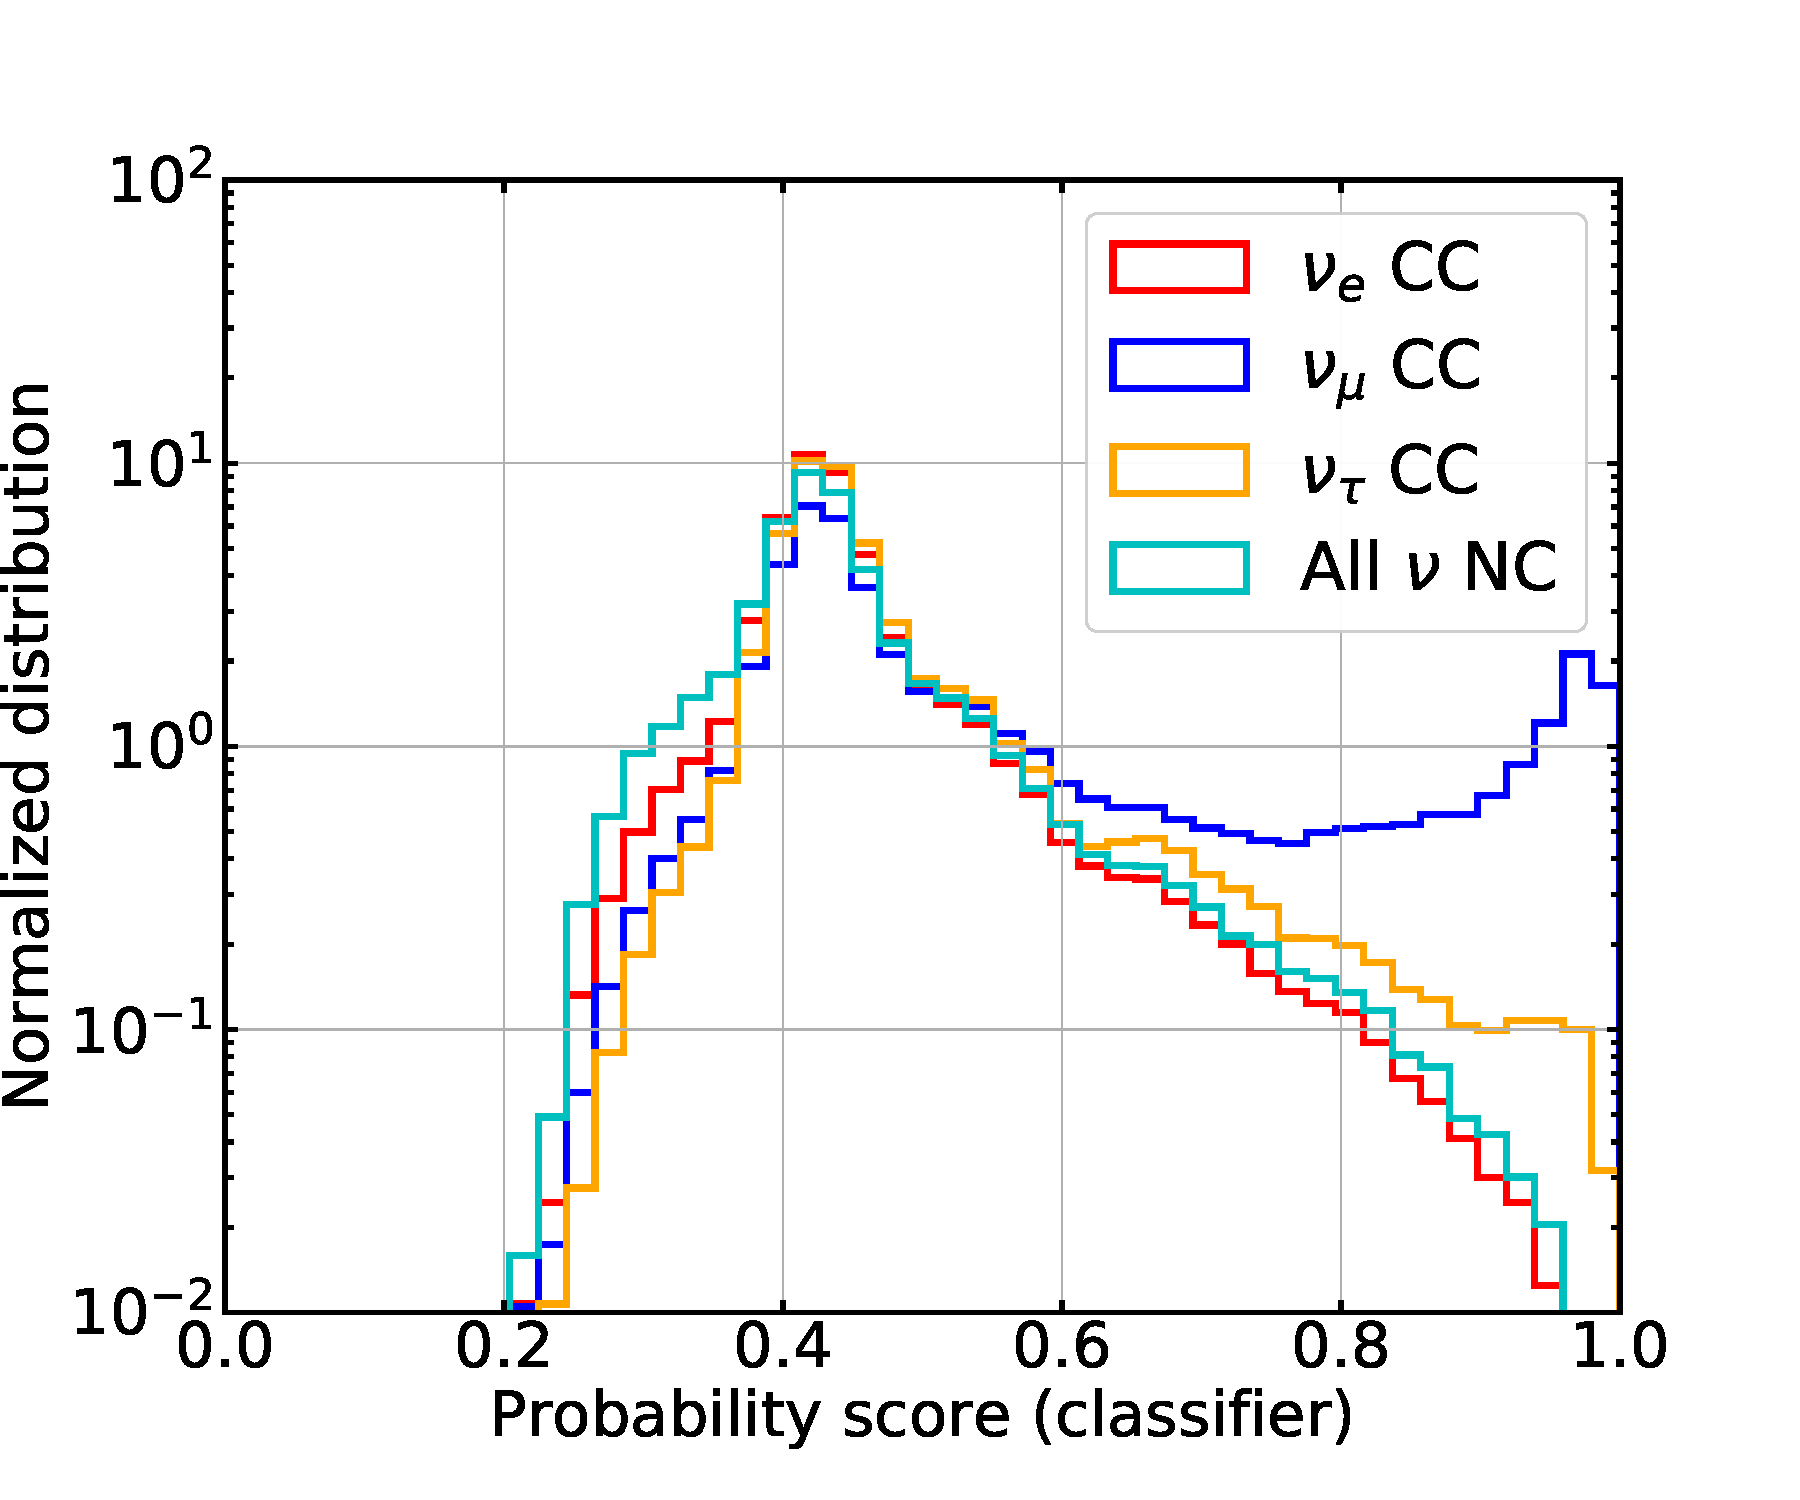
\includegraphics[width=0.8\linewidth]{figures/icecube/classification/bdt_score_normalized.pdf}
    \tikzsetnextfilename{bdt_score_normalized}%
\begin{tikzpicture}

    \pgfplotstableread{figures/icecube/classification/gbm_normalized_nu_hists_nufit22.csv}\table
    \begin{axis}[
        xmin=0,xmax=1.0,
        xmajorgrids, ymajorgrids,
        width=0.7\linewidth,
        height=0.6\linewidth,
        ymode=log,
        ymin=1e-02, ymax=100,
        ylabel=distribution density,
        xlabel=BDT score,
        legend cell align={left},
        legend columns=2,
    ]

    \addplot[const plot, nue_color, thick] table [x=bin_edges, y=nue_cc] from \table;
    \addlegendentry{$\nu_e + \bar{\nu}_e$, CC}
    \addplot[const plot, numu_color, thick] table [x=bin_edges, y=numu_cc] from \table;
    \addlegendentry{$\nu_\mu + \bar{\nu}_\mu$, CC}
    \addplot[const plot, nutau_color, thick] table [x=bin_edges, y=nutau_cc] from \table;
    \addlegendentry{$\nu_\tau + \bar{\nu}_\tau$, CC}
    \addplot[const plot, nc_color, thick] table [x=bin_edges, y=nu_nc] from \table;
    \addlegendentry{all $\nu$, NC}
    
    \end{axis}
\end{tikzpicture}

    \caption{PID score distribution for simulated neutrino events at the final level of the event selection, weighted according to the HKKM flux model~\cite{Honda:2015fha} and neutrino oscillations with \textsc{NuFit}~4.0\cite{nufit40} global fit parameters, normalized to unity. The BDT score ranges from the most cascade-like at 0 to the most track-like event signature at 1.}
    \label{fig:pid-score}
\end{figure}

\subsection{Final Sample Selection and Binning}
\label{sec:final-sample-binning}
After the reconstruction and classification step, several final cut variables are applied to reduce the background of atmospheric muons to only a few percent, and to remove a small number of events from data containing coincident muons.
These cuts are:
\begin{itemize}
    \item The reconstruction of energy and zenith angle has to be successful.
This requires, in particular, that at least five hits remain after the hit cleaning procedure described in \refsec{santa}.
    \item The reconstructed energy should be in the range between \SI{6}{\giga\electronvolt} and \SI{156}{\giga\electronvolt}.
    \item Require a minimum PID score (see \refsec{pid}) of 0.55 to only include at least somewhat track-like events.
    \item Reconstructed $\cos(\theta_z) < 0.1$ to remove events that enter the detector from above the horizon.
    \item Require a minimum goodness-of-fit of the zenith reconstruction with $\chi^2_{\mathrm{mod}}/\mathrm{d.o.f.} < 50$.
    \item A tighter cut on the L4 muon BDT score (see \refsec{level4-selection}) of $P_\nu > 0.97$.
    \item Fewer than eight hits in the outermost strings of the IceCube array, and a positive "z-travel" value for hits in the uppermost 15 layers of DOMs in the (non-DeepCore) IceCube array.
The "z-travel" value for a given sequence of hits is calculated by subtracting the mean value of the z-coordinate of the first quartile of hits from the mean z-coordinate of all hits.
\end{itemize}

\begin{figure}
    \centering
    \tikzsetnextfilename{z_travel_top15}%
\begin{tikzpicture}
    \pgfplotstableread{figures/icecube/selection/Level7/z_travel_top15.csv}\table

    \begin{axis}[
    	xmin=-150,xmax=150,
        xmode=normal,
        xmajorgrids, ymajorgrids,
        width=0.45\linewidth,
        % ylabel style={at={(-0.15,0.5)}},
        height=0.55\linewidth,
        legend cell align={left},
        legend columns=3,
        ymode=log,
        ymin=2e-9, ymax=5e-6,
        y filter/.expression={y < 1e-10 ? ln(1e-11) : ln(y)},
        ylabel=rate (Hz),
        xlabel=z-travel in upper 15 IceCube DOMs
    ]
	
    \ploterrorband[muon_color]{muon}{1}
    \addlegendentry{atm. muons}

    \ploterrorband[nue_color]{nuenuebar}{1}
    \addlegendentry{$\nu_e + \bar{\nu}_e$}
    
    \ploterrorband[numu_color]{numunumubar}{1}
    \addlegendentry{$\nu_\mu + \bar{\nu}_\mu$}
    
    \ploterrorband[nutau_color]{nutaunutaubar}{1}
    \addlegendentry{$\nu_\tau + \bar{\nu}_\tau$}
   
    
    \ploterrorband{total_mc}{1}
    \addlegendentry{total MC}
	
	
	% draw cut
    % use "axis cs" to give coordinates in the data coordinate system!
    \draw[thick,dashed] (axis cs:0,1e-9) -- (axis cs:0,5e-5);
    \draw[-stealth, very thick] (axis cs:0,3e-7)  -- node[anchor=south]{\footnotesize\sffamily signal} (axis cs:50,3e-7);
    
    \addplot[
        mark=*,
        mark options={scale=0.5, fill=black},
        black,
        only marks,
        error bars/.cd,
        x dir=none,
        y dir=both,
        y explicit
    ] table [x=bin_midpoints, y=data, y error=data__err]  from \table;
    \addlegendentry{data}
	
	\end{axis}
\end{tikzpicture}

    \caption{Distribution of the "z-travel" variable calculated for the uppermost 15 layers of IceCube DOMs. Only events with at least 4 hits in the uppermost 15 layers of DOMs are included in the histogram.}
    \label{fig:z_travel_distribution}
\end{figure}

% \begin{figure}
%     \centering
%     \tikzsetnextfilename{santa_chi2dof}%
\begin{tikzpicture}
    \pgfplotstableread{figures/icecube/selection/Level7/santa_chi2dof.csv}\table
    \begin{groupplot}[
        xmin=3,xmax=300,
        xmode=log,
        xmajorgrids, ymajorgrids,
        width=0.45\linewidth,
        ylabel style={at={(-0.15,0.5)}},
        group/.cd,
        group size=1 by 2,
        xticklabels at=edge bottom,
        vertical sep=10pt
        ]
    \nextgroupplot[
        height=0.3\linewidth,
        legend cell align={left},
        legend columns=3,
        legend to name=santa_chi2dof_legend,
        ymode=log,
        ymin=2e-8, ymax=5e-3,
        ylabel=rate (Hz),
    ]

    \ploterrorband[muon_color]{muon}{1}
    \addlegendentry{atm. muons}

    \ploterrorband[nue_color]{nuenuebar}{1}
    \addlegendentry{$\nu_e + \bar{\nu}_e$}
    
    \ploterrorband[numu_color]{numunumubar}{1}
    \addlegendentry{$\nu_\mu + \bar{\nu}_\mu$}
    
    \ploterrorband[nutau_color]{nutaunutaubar}{1}
    \addlegendentry{$\nu_\tau + \bar{\nu}_\tau$}
    
    % alternative  event breakdown by interaction
    
    % \ploterrorband[nue_color]{nue_ccnuebar_cc}{1}
    % \addlegendentry{$\nu_e + \bar{\nu}_e$, CC}
    
    % \ploterrorband[numu_color]{numu_ccnumubar_cc}{1}
    % \addlegendentry{$\nu_\mu + \bar{\nu}_\mu$, CC}
    
    % \ploterrorband[nutau_color]{nutau_ccnutaubar_cc}{1}
    % \addlegendentry{$\nu_\tau + \bar{\nu}_\tau$, CC}
    
    % \ploterrorband[nc_color]{nuall_ncnuallbar_nc}{1}
    % \addlegendentry{all $\nu$, NC}
    
    \ploterrorband{total_mc}{1}
    \addlegendentry{total MC}

    % draw cut
    % use "axis cs" to give coordinates in the data coordinate system!
    \draw[thick,dashed] (axis cs:50,1e-8) -- (axis cs:50,5e-4);
    \draw[-stealth, very thick] (axis cs:50,1e-7)  -- node[anchor=south]{\footnotesize\sffamily signal} (axis cs:20,1e-7);
    
    \addplot[
        mark=*,
        mark options={scale=0.5, fill=black},
        black,
        only marks,
        error bars/.cd,
        x dir=none,
        y dir=both,
        y explicit
    ] table [x=bin_midpoints, y=data, y error=data__err]  from \table;
    \addlegendentry{data}


    \nextgroupplot[
        height=0.2\linewidth,
        ymin=0.8, ymax=1.2,
        ylabel=data/MC ratio,
        xlabel=SANTA $\chi^2 / \mathrm{d.o.f.}$\strut
    ]
    
    \ploterrorband{data_mc_ratio}{1}
    %\plotratioerrorband[muon_color]{muon}{total_mc}
    \end{groupplot}
\end{tikzpicture}

%     \caption{Distribution of the SANTA goodness-of-fit variable.}
%     \label{fig:santa_chi2dof_distribution}
% \end{figure}


\begin{figure*}
    \centering
    \ref{reco_coszen_legend}\par
    \tikzsetnextfilename{santa_chi2dof}%
\begin{tikzpicture}
    \pgfplotstableread{figures/icecube/selection/Level7/santa_chi2dof.csv}\table
    \begin{groupplot}[
        xmin=3,xmax=300,
        xmode=log,
        xmajorgrids, ymajorgrids,
        width=0.45\linewidth,
        ylabel style={at={(-0.15,0.5)}},
        group/.cd,
        group size=1 by 2,
        xticklabels at=edge bottom,
        vertical sep=10pt
        ]
    \nextgroupplot[
        height=0.3\linewidth,
        legend cell align={left},
        legend columns=3,
        legend to name=santa_chi2dof_legend,
        ymode=log,
        ymin=2e-8, ymax=5e-3,
        ylabel=rate (Hz),
    ]

    \ploterrorband[muon_color]{muon}{1}
    \addlegendentry{atm. muons}

    \ploterrorband[nue_color]{nuenuebar}{1}
    \addlegendentry{$\nu_e + \bar{\nu}_e$}
    
    \ploterrorband[numu_color]{numunumubar}{1}
    \addlegendentry{$\nu_\mu + \bar{\nu}_\mu$}
    
    \ploterrorband[nutau_color]{nutaunutaubar}{1}
    \addlegendentry{$\nu_\tau + \bar{\nu}_\tau$}
    
    % alternative  event breakdown by interaction
    
    % \ploterrorband[nue_color]{nue_ccnuebar_cc}{1}
    % \addlegendentry{$\nu_e + \bar{\nu}_e$, CC}
    
    % \ploterrorband[numu_color]{numu_ccnumubar_cc}{1}
    % \addlegendentry{$\nu_\mu + \bar{\nu}_\mu$, CC}
    
    % \ploterrorband[nutau_color]{nutau_ccnutaubar_cc}{1}
    % \addlegendentry{$\nu_\tau + \bar{\nu}_\tau$, CC}
    
    % \ploterrorband[nc_color]{nuall_ncnuallbar_nc}{1}
    % \addlegendentry{all $\nu$, NC}
    
    \ploterrorband{total_mc}{1}
    \addlegendentry{total MC}

    % draw cut
    % use "axis cs" to give coordinates in the data coordinate system!
    \draw[thick,dashed] (axis cs:50,1e-8) -- (axis cs:50,5e-4);
    \draw[-stealth, very thick] (axis cs:50,1e-7)  -- node[anchor=south]{\footnotesize\sffamily signal} (axis cs:20,1e-7);
    
    \addplot[
        mark=*,
        mark options={scale=0.5, fill=black},
        black,
        only marks,
        error bars/.cd,
        x dir=none,
        y dir=both,
        y explicit
    ] table [x=bin_midpoints, y=data, y error=data__err]  from \table;
    \addlegendentry{data}


    \nextgroupplot[
        height=0.2\linewidth,
        ymin=0.8, ymax=1.2,
        ylabel=data/MC ratio,
        xlabel=SANTA $\chi^2 / \mathrm{d.o.f.}$\strut
    ]
    
    \ploterrorband{data_mc_ratio}{1}
    %\plotratioerrorband[muon_color]{muon}{total_mc}
    \end{groupplot}
\end{tikzpicture}

    \tikzsetnextfilename{reco_coszen_l5}%
\begin{tikzpicture}
    \pgfplotstableread{figures/icecube/selection/Level7/reco_coszen.csv}\table
    \begin{groupplot}[
        xmin=-1.1,xmax=1.1,
        xmode=normal,
        xmajorgrids, ymajorgrids,
        width=0.45\linewidth,
        ylabel style={at={(-0.15,0.5)}},
        group/.cd,
        group size=1 by 2,
        xticklabels at=edge bottom,
        vertical sep=10pt
        ]
    \nextgroupplot[
        height=0.3\linewidth,
        legend cell align={left},
        legend columns=-1,
        legend to name=reco_coszen_legend,
        ymode=log,
        ymin=2e-7, ymax=5e-4,
        ylabel=rate (Hz),
        % add magic filter to correctly handle empty bins in logarithmic y-axes:
        % If a bin-count is too low or zero, it would cause the line to be
        % interrupted, which creates artefacts and ugliness. Instead, we replace
        % these bin-counts with values that are just below the axis limit.
        % Because of the way pgfplots works, the input is the raw number but the
        % output has to be the log. Weird, I know.
        y filter/.expression={y < 8.7587858920556e-09 ? ln(8.758785892055601e-10) : ln(y)}
    ]

    \ploterrorband[muon_color]{muon}{1}
    \addlegendentry{atm. muons}

    \ploterrorband[nue_color]{nuenuebar}{1}
    \addlegendentry{$\nu_e + \bar{\nu}_e$}

    \ploterrorband[numu_color]{numunumubar}{1}
    \addlegendentry{$\nu_\mu + \bar{\nu}_\mu$}

    \ploterrorband[nutau_color]{nutaunutaubar}{1}
    \addlegendentry{$\nu_\tau + \bar{\nu}_\tau$}


    % alternative event breakdown by interaction
    % \ploterrorband[nue_color]{nue_ccnuebar_cc}{1}
    % \addlegendentry{$\nu_e + \bar{\nu}_e$, CC}
    %
    % \ploterrorband[numu_color]{numu_ccnumubar_cc}{1}
    % \addlegendentry{$\nu_\mu + \bar{\nu}_\mu$, CC}
    %
    % \ploterrorband[nutau_color]{nutau_ccnutaubar_cc}{1}
    % \addlegendentry{$\nu_\tau + \bar{\nu}_\tau$, CC}
    %
    % \ploterrorband[nc_color]{nuall_ncnuallbar_nc}{1}
    % \addlegendentry{all $\nu$, NC}

    \ploterrorband{total_mc}{1}
    \addlegendentry{total MC}

    \ploterrorbar{data}
    \addlegendentry{data}


    % draw cut
    % use "axis cs" to give coordinates in the data coordinate system!
    \draw[thick,dashed] (axis cs:0.1,1e-9) -- (axis cs:0.1,5e-4);
    \draw[-stealth, very thick] (axis cs:0.1,1e-4)  -- node[anchor=south]{\footnotesize\sffamily signal} (axis cs:-0.4,1e-4);
    
    \nextgroupplot[
        height=0.2\linewidth,
        ymin=0.5, ymax=1.5,
        ylabel=data/MC ratio,
        xlabel=reconstructed $\cos(\theta_{\mathrm{zenith}})$\strut
    ]

    \ploterrorband{data_mc_ratio}{1}
    \end{groupplot}
\end{tikzpicture}

    \caption{Distribution of the SANTA goodness-of-fit variable and the reconstructed zenith angle at L5 of the event selection process.}
    \label{fig:final_cut_vars_l5}
\end{figure*}

The cuts on energy, zenith angle, and PID define the range of the binning that will be used in the analysis.
The cut on the zenith angle in particular is applied not only to reduce the background of atmospheric muons, but also to remove the phase space of neutrino events where muons that are produced in the same air shower that also produced the neutrino cause it to be vetoed by the muon filter cuts.
This effect is referred to as the "self-veto" effect and would lead to a disagreement between data and simulation since coincident muons are never simulated.
The distribution of the cosine of the reconstructed zenith angle is shown in the right panel of \reffig{final_cut_vars_l5}, and it is apparent from the distributions that atmospheric muons dominate in the region of down-going events.

The requirement on the SANTA goodness-of-fit not only ensures that the included events are well-reconstructed, but also reduces the fraction of muons in the sample, as can be seen from the distributions shown in the left panel of \reffig{final_cut_vars_l5}.
The number of hits on the outermost strings and the "z-travel" variable calculated for hits in the uppermost 15 layers of IceCube DOMs are indicators of muons that hit the detector within the trigger window of a neutrino event.
Such coincidences are entirely absent in simulation, which becomes especially apparent in the distribution of the "z-travel" variable shown in \reffig{z_travel_distribution}, where a negative value indicates a down-going signal.
After the application of all these cuts, the data sample consists of 21,914 well-reconstructed, track-like events with an expected background from atmospheric muons of only $\sim 2\%$ as shown in table~\ref{tab:muon-rejection-cut-rates}.
For the purpose of the oscillation measurements presented in this work, both data and simulation sets are binned in reconstructed energy ($E_{\rm reco}$), cosine of the reconstructed zenith angle ($\cos(\theta_z)$), and PID as follows:

\begin{itemize}
    \item $E_{\rm reco}$: 11 bins spanning the range from 6.31~GeV to 158.49~GeV, the two bins with the highest energy are merged.
    \item $\cos(\theta_z)$: 10 bins spanning the range from -1 to 0.1
    \item PID: One bin between 0.55 and 0.75, and one bin between 0.75 and 1.0.
\end{itemize}

The lower PID bin between 0.55 and 0.75 consists to 69\%  (pre-fit MC estimate) of charged-current $\nu_\mu + \bar{\nu}_\mu$ events and is referred to as the \emph{mixed} channel, while the higher PID channel between 0.75 and 1.0 consists to 94\% of charged-current $\nu_\mu + \bar{\nu}_\mu$ events and is referred to as the \emph{tracks} channel.
The expectation values of the histogram in both PID channels is shown in \reffig{nominal-hist-null-hypo} at current global best-fit parameters for standard three-flavor oscillations.
The expectation values are calculated from Monte-Carlo (MC) simulation that is described in detail in \refsec{event-simulation}.
The detailed breakdown of event counts in the final data sample by particle type and PID channel is given in \reftab{event-rate}.

\begin{figure}
    \centering
    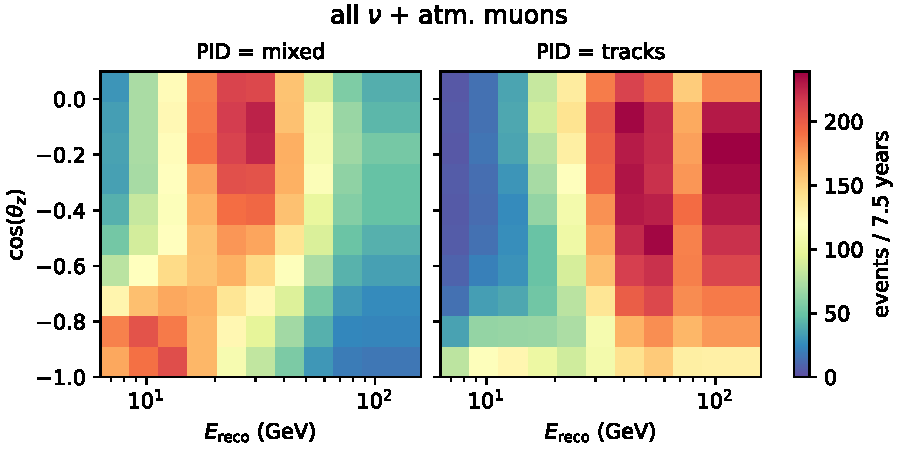
\includegraphics[width=0.95\textwidth]{figures/measurement/simulation_and_data/binning/plot_maps_total.pdf}
    \caption{Expected event counts in 7.5 years of live time assuming no sterile mixing and NuFit~4.0~\cite{nufit40} global best fit parameters at Normal Ordering.}
    \label{fig:nominal-hist-null-hypo}
\end{figure}

\begin{table}
\caption{Successively applied cuts on the data sample. The bottom row corresponds to the final rates in the sample after all cuts have been applied. The total rate of the data and simulation does not match, which is expected since there is a large amount of uncertainty in the total normalization. Muon contamination is the muon rate divided by the total event rate. Numbers calculated at the NuFit 4.0 global best-fit point.}
\centering
\begin{tabular}{@{}lrrrr@{}}\toprule
& \multicolumn{3}{c}{rate ($\mu$Hz)} & \\ \cmidrule{2-4}
condition                              & {$\nu$ (sim)} & {$\mu$ (sim)} & {data} & {$\mu$ fraction} \\ \midrule
has SANTA reconstruction         & 957  & 314  & 1183 & 24.7 \%  \\
$\SI{6}{\giga\electronvolt} < E_\mathrm{reco}  < \SI{156}{\giga\electronvolt}$         & 862  & 311  & 1095 & 26.5 \%  \\
BDT score $>0.55$                      & 232  & 117  &  336 & 33.5 \%  \\
$\cos(\theta_{\mathrm{reco}}) < 0.1$   & 175  &  17  &  177 & 8.8 \%   \\
SANTA $\chi^2/\mathrm{d.o.f.} < 50$    & 164  &  12  &  161 & 6.6 \%   \\
L4 muon $\nu$ prob $> 0.97$            & 101  &   2  &   93 & 2.1 \% \\
\midrule\addlinespace
coinc. $\mu$ cuts (final rate) & \textbf{101} & \textbf{2} & \textbf{93} & \textbf{2.1 \%} \\ \bottomrule
\end{tabular}
\label{tab:muon-rejection-cut-rates}
\end{table}

%\begin{figure*}
%    \centering
%    \ref{reco_coszen_prefit_legend}\par
%    \begin{tikzpicture}
    \pgfplotstableread{figures/icecube/selection/final_sample_prefit/reco_coszen.csv}\table
    \begin{groupplot}[
        xmin=-1.055,xmax=0.15500000000000003,
        xmode=normal,
        xmajorgrids, ymajorgrids,
        width=0.45\linewidth,
        ylabel style={at={(-0.15,0.5)}},
        group/.cd,
        group size=1 by 2,
        xticklabels at=edge bottom,
        vertical sep=10pt
        ]
    \nextgroupplot[
        height=0.3\linewidth,
        legend cell align={left},
        legend columns=-1,
        legend to name=reco_coszen_prefit_legend,
        ymode=log,
        ymin=2.670138976548827e-09, ymax=3e-5,
        ylabel=rate (Hz),
        ytick distance=1e1,
        % add magic filter to correctly handle empty bins in logarithmic y-axes:
        % If a bin-count is too low or zero, it would cause the line to be
        % interrupted, which creates artefacts and ugliness. Instead, we replace
        % these bin-counts with values that are just below the axis limit.
        % Because of the way pgfplots works, the input is the raw number but the
        % output has to be the log. Weird, I know.
        y filter/.expression={y < 2.670138976548827e-09 ? ln(2.6701389765488273e-10) : ln(y)}
    ]

    \ploterrorband[muon_color]{muon}{1}
    \addlegendentry{atm. muons}

    \ploterrorband[nue_color]{nuenuebar}{1}
    \addlegendentry{$\nu_e + \bar{\nu}_e$}

    \ploterrorband[numu_color]{numunumubar}{1}
    \addlegendentry{$\nu_\mu + \bar{\nu}_\mu$}

    \ploterrorband[nutau_color]{nutaunutaubar}{1}
    \addlegendentry{$\nu_\tau + \bar{\nu}_\tau$}


    % alternative event breakdown by interaction
    % \ploterrorband[nue_color]{nue_ccnuebar_cc}{1}
    % \addlegendentry{$\nu_e + \bar{\nu}_e$, CC}
    %
    % \ploterrorband[numu_color]{numu_ccnumubar_cc}{1}
    % \addlegendentry{$\nu_\mu + \bar{\nu}_\mu$, CC}
    %
    % \ploterrorband[nutau_color]{nutau_ccnutaubar_cc}{1}
    % \addlegendentry{$\nu_\tau + \bar{\nu}_\tau$, CC}
    %
    % \ploterrorband[nc_color]{nuall_ncnuallbar_nc}{1}
    % \addlegendentry{all $\nu$, NC}

    \ploterrorband{total_mc}{1}
    \addlegendentry{total MC}

    \ploterrorbar{data}
    \addlegendentry{data}

    \nextgroupplot[
        height=0.2\linewidth,
        ymin=-0.1, ymax=1.8,
        ylabel=rate/total MC,
        xlabel=reconstructed $\cos(\theta_{\mathrm{zenith}})$
    ]
   
    \ploterrorbar{data_mc_ratio}
    \plotratioerrorband[muon_color]{muon}{total_mc}
    \plotratioerrorband[nue_color]{nuenuebar}{total_mc}
    \plotratioerrorband[numu_color]{numunumubar}{total_mc}
    \plotratioerrorband[nutau_color]{nutaunutaubar}{total_mc}
    
    \end{groupplot}
\end{tikzpicture}

%    \tikzsetnextfilename{final_level_prefit_reco_energy}%
\begin{tikzpicture}
    \pgfplotstableread{figures/icecube/selection/final_sample_prefit/reco_energy.csv}\table
    \begin{groupplot}[
        xmin=5.362591587787688,xmax=185.61920737481475,
        xmode=log,
        xmajorgrids, ymajorgrids,
        width=0.45\linewidth,
        ylabel style={at={(-0.15,0.5)}},
        group/.cd,
        group size=1 by 2,
        xticklabels at=edge bottom,
        vertical sep=10pt
        ]
    \nextgroupplot[
        height=0.3\linewidth,
        legend cell align={left},
        legend columns=-1,
        legend to name=prefit_reco_energy_legend,
        ymode=log,
        ymin=2.670138976548827e-09, ymax=3e-5,
        ylabel=rate (Hz),
        ytick distance=1e1,
        % add magic filter to correctly handle empty bins in logarithmic y-axes:
        % If a bin-count is too low or zero, it would cause the line to be
        % interrupted, which creates artefacts and ugliness. Instead, we replace
        % these bin-counts with values that are just below the axis limit.
        % Because of the way pgfplots works, the input is the raw number but the
        % output has to be the log. Weird, I know.
        y filter/.expression={y < 9.437724466286084e-10 ? ln(9.437724466286085e-11) : ln(y)}
    ]

    \ploterrorband[muon_color]{muon}{1}
    \addlegendentry{atm. muons}

    \ploterrorband[nue_color]{nuenuebar}{1}
    \addlegendentry{$\nu_e + \bar{\nu}_e$}

    \ploterrorband[numu_color]{numunumubar}{1}
    \addlegendentry{$\nu_\mu + \bar{\nu}_\mu$}

    \ploterrorband[nutau_color]{nutaunutaubar}{1}
    \addlegendentry{$\nu_\tau + \bar{\nu}_\tau$}


    % alternative event breakdown by interaction
    % \ploterrorband[nue_color]{nue_ccnuebar_cc}{1}
    % \addlegendentry{$\nu_e + \bar{\nu}_e$, CC}
    %
    % \ploterrorband[numu_color]{numu_ccnumubar_cc}{1}
    % \addlegendentry{$\nu_\mu + \bar{\nu}_\mu$, CC}
    %
    % \ploterrorband[nutau_color]{nutau_ccnutaubar_cc}{1}
    % \addlegendentry{$\nu_\tau + \bar{\nu}_\tau$, CC}
    %
    % \ploterrorband[nc_color]{nuall_ncnuallbar_nc}{1}
    % \addlegendentry{all $\nu$, NC}

    \ploterrorband{total_mc}{1}
    \addlegendentry{total MC}

    \ploterrorbar{data}
    \addlegendentry{data}

    \nextgroupplot[
        height=0.2\linewidth,
        ymin=-0.1, ymax=1.8,
        ylabel=rate/total MC,
        xlabel=reconstructed energy (GeV)
    ]

    \ploterrorbar{data_mc_ratio}
    \plotratioerrorband[muon_color]{muon}{total_mc}
    \plotratioerrorband[nue_color]{nuenuebar}{total_mc}
    \plotratioerrorband[numu_color]{numunumubar}{total_mc}
    \plotratioerrorband[nutau_color]{nutaunutaubar}{total_mc}

    \end{groupplot}
\end{tikzpicture}

%    \caption{Distributions of reconstructed energy and zenith angle at the final level of the event selection, calculated assuming \textsc{NuFit}~4.0\cite{nufit40} global best fit oscillation parameters.}
%    \label{fig:pre-fit-energy-coszen}
%\end{figure*}


\begin{table}[htb]
\centering
\caption{Expected event rate with 8 years livetime broken down in event types and PID bins, calculated at NuFit~4.0 global best fit parameters.}
\label{tab:event-rate}
\begin{tabular}{lcrS} \toprule
Type  & PID & Event Count & {Rate ($\mathrm{\mu Hz}$)} \\ \midrule
All MC & mixed  &   11428 &   48.3\\
All MC & tracks &   12238 &   51.7\\ \midrule
${\nu_{\rm all}} + {\bar\nu_{\rm all}} \, {\rm NC} $ & mixed  &     943 &    4.0 \\
${\nu_e} + {\bar\nu_e} \, {\rm CC}                 $ & mixed  &    1704 &    7.2 \\
${\nu_\mu} + {\bar\nu_\mu} \, {\rm CC}             $ & mixed  &    7901 &   33.4 \\
${\nu_\tau} + {\bar\nu_\tau} \, {\rm CC}           $ & mixed  &     470 &    2.0 \\
muons                                                & mixed  &     410 &    1.7 \\
\midrule
${\nu_{\rm all}} + {\bar\nu_{\rm all}} \, {\rm NC} $ & tracks &     171 &    0.7 \\
${\nu_e} + {\bar\nu_e} \, {\rm CC}                 $ & tracks &     294 &    1.2 \\
${\nu_\mu} + {\bar\nu_\mu} \, {\rm CC}             $ & tracks &   11517 &   48.7 \\
${\nu_\tau} + {\bar\nu_\tau} \, {\rm CC}           $ & tracks &     162 &    0.7 \\
muons                                                & tracks &      93 &    0.4 \\
\bottomrule
\end{tabular}
\end{table}


\subsubsection{Muon Smearing}
\label{section:muon_kde}

After all the filtering steps described in section~\ref{sec:data-processing}, the muon contamination of the data sample is reduced to $\sim 2\%$ of the sample.
This reduces the statistics of muon simulation so much, that the resulting histograms become very sparse as shown in figure~\ref{fig:muon-template-no-kde}.
Such sparse histograms, in which single MC events have to serve as a stand-in for several real data events, are a poor template for what can be expected in data.
To produce a more realistic expectation of the bin counts, the muon histograms are smeared using KDEs as shown in figure \ref{fig:muon-template-with-kde}.
Since the KDE operates on events on the entire zenith and energy range, including events that fall outside the analysis binning, some events bleed into the highest $\cos(\theta_z)$ bin from further above the horizon.
The KDE kernel is mirrored at $\cos(\theta_z) = -1$ to avoid spurious disappearance of events at the edge.
The smeared muon histogram is added to the expectation values from the neutrino MC simulation to estimate the total expectation value in every bin shown in \reffig{nominal-hist-null-hypo}.

\begin{figure}[H]
    \centering
    \begin{subfigure}{0.8\textwidth}
        \centering
        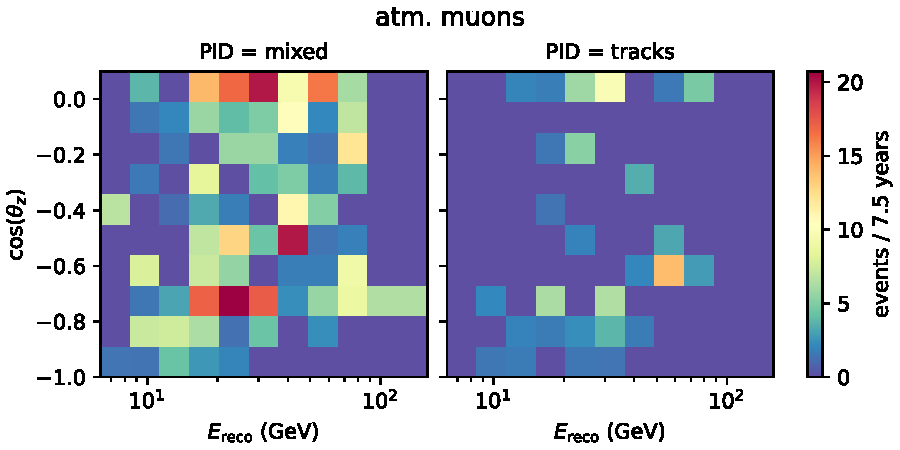
\includegraphics[width=\textwidth,trim={0 0 0 0.6cm},clip]{figures/measurement/systematics/muons/muon_hist_no_kde.pdf}
        \caption{Without KDE smoothing}
        \label{fig:muon-template-no-kde}
    \end{subfigure}
    \begin{subfigure}{0.8\textwidth}
        \centering
        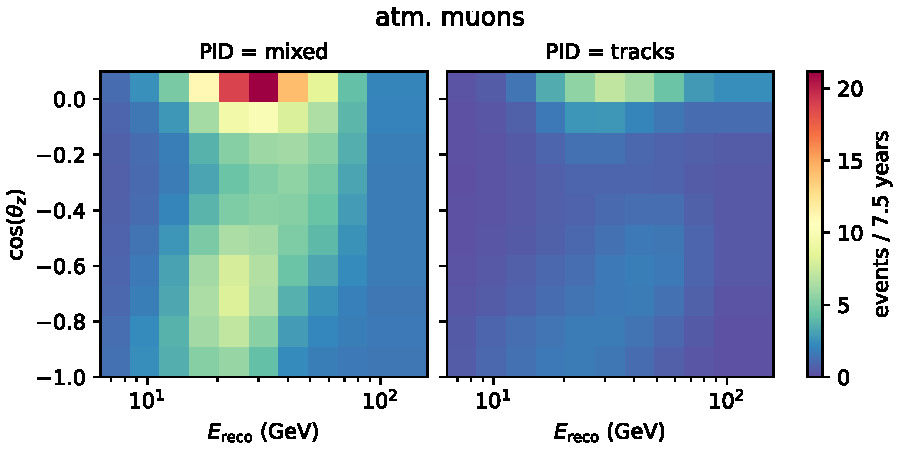
\includegraphics[width=\textwidth,trim={0 0 0 0.6cm},clip]{figures/measurement/systematics/muons/plot_maps_muon.pdf}
        \caption{With KDE smoothing}
        \label{fig:muon-template-with-kde}
    \end{subfigure}

    \caption{Muon template before (top) and after (bottom) the application of KDE smoothing. The shown values are the average of 20 KDE evaluations on different bootstrap samples.}
    \label{fig:muon-kde-smoothing}
\end{figure}

\section{Implementation of systematic uncertainties}
\subsection{Variation of Detector Properties}
\label{sec:detector-unc}
Systematic uncertainties on the detector properties that need to be taken into account are the overall optical efficiency of the DOMs as well as the properties of the surrounding ice.
The parametrization and priors of each of these properties are informed by IceCube calibration studies.
\begin{itemize}
    \item DOM efficiency: A factor that scales the probability that a photon hitting the PMT of a DOM will produce a photo-electron that is measured by the electronics.
Nominal value is 1, prior standard deviation is 10\%.
    \item Hole ice: Two parameters describe the effect of the optical properties of the column of re-frozen ice within the bore holes in which the strings have been deployed.
The details of this parametrization is described below.
    \item Bulk ice: The over-all absorption and scattering coefficients of all ice layers are multiplied by a scaling factor.
The nominal value for ice absorption is 1.0 with a prior standard deviation of 5\%.
The nominal value for ice scattering is 1.05 with a prior standard deviation of 10\%.
\end{itemize}

In total, the uncertainties on the detector properties are modeled by five  parameters, one for the DOM efficiency, two for the hole ice model and two for the bulk ice uncertainty.
To model the effect of these parameters on the analysis histogram, several MC sets at different variations of DOM efficiency, hole ice, and bulk ice parameters are produced.
These MC sets are used to find a parametrization that will model how the distribution of events in energy, zenith and PID will change as a function of these parameters.

\subsubsection{DOM efficiency calibration}
\label{sec:domeff-calibration}
As described in \refsec{dom-daq}, the DOMs contain LEDs that are used to calibrate the detector \emph{in-situ}. However, these LEDs are not calibrated with respect to their absolute brightness and therefore are not suited for the calibration of the optical efficiency of the DOMs. Instead, minimally ionizing muons that are produced in air showers are used as a light source with a known brightness. The calibration is performed using a sample of events that pass the \emph{Minimum Bias Trigger}\cite{icecube_detector_17} and in which the reconstructed muon track stops within the instrumented volume of IceCube. The DOM efficiency is estimated by comparing the observed charges in the DOMs and the light expectation from the reconstructed muons. Multiple such calibration studies have been run \sidecite{domeff_nick}\sidecite{domeff_jake} and found variations in the optical efficiency of approximately 10\%, which is used as a prior for the measurements presented in this work.

\subsubsection{Hole Ice Parametrization}
\label{sec:hole-ice-parametrization}

The bore holes in which IceCube's strings have been deployed were drilled using hot water to melt a column of ice into which the strings with their attached optical sensors could be lowered.
This water column re-froze after deployment to form what is referred to as \emph{hole ice}\sidecite{Fiedlschuster:2019unl}.
Camera observations of this re-freezing process suggest that the hole ice is transparent near the edges of be hole and contains a bubble column in its center\sidecite{rongen2016measuring}.
The bubble column has a much shorter scattering length than the surrounding bulk ice and therefore decreases the probability of a photon entering a DOM directly from below.
The effect of the re-frozen ice column surrounding the strings can be modeled as a modification to the optical efficiency of the DOMs as a function of the incident angle of incoming photons.
In the past, many different angular acceptance curves have been produced from \emph{in-situ} calibration measurements\cite{flasher_calibration}, the best fit results of previous DeepCore oscillation analyses, in addition to the laboratory measurements that have been made in water tanks before the deployment of IceCube.
For the analysis presented in this work, a two-dimensional parametrization was developed that can approximate any of these hole ice models such that it can be used as a \emph{unified} hole ice model.
To do this, all previous angular acceptance curves are evaluated as a function of the cosine of the photon incidence angle, $\cos(\eta)$, at 100 points over the entire valid domain between -1 and 1, where 1 represents a photon entering a DOM directly from below.
The curves are furthermore normalized to an area of 1 to avoid affecting the total observed charge.
Using Principal Component Analysis\sidecite{pca}, the variations between the different models are decomposed into a mean and the most important components that explain the variance between models.
It was found that the two most important components, $p_0$ and $p_1$, describe all known hole ice models adequately.
Their effect is shown in \reffig{hole-ice-parametrization} as variations with the acceptance curve that is used as the baseline in this analysis.
The right panel of \reffig{hole-ice-parametrization} also shows where the older hole ice models are located in the space spanned by $p_0$ and $p_1$.
The laboratory measurement, which did not include any hole ice effects, notably lies far outside of the region of all other hole ice models that are all produced \emph{in-situ}.

\begin{figure*}
    \centering
    \tikzsetnextfilename{hole_ice_p0_p1}%
\begin{tikzpicture}

\pgfplotstableread{figures/measurement/systematics/detector/hole_ice/angsens_example_fluct.csv}\table
\pgfplotstableread{figures/measurement/systematics/detector/hole_ice/all_acceptance_curves.csv}\acceptancecurves

\begin{axis}[
        width=0.45\linewidth, height=0.4\linewidth,
		xmajorgrids, ymajorgrids,
		xlabel=$\cos(\eta)$, ylabel=relative optical efficiency,
		legend style={at={(0.02,0.95)}, anchor=north west},
        ytick distance=0.2,
	]
    \addplot[black, thick] table [x=cos_theta, y=baseline] \acceptancecurves;
    \addlegendentry{baseline}
    
    \addplot[vermilion, thick] table [x=cos_theta, y=nominal] \acceptancecurves;
    \addlegendentry{laboratory}
    
    % \addplot[bluishgreen, thick] table [x=cos_theta, y=bfp_three_flav] \acceptancecurves;
    % \addlegendentry{best fit}
    
    \addplot[blue, thin, name path=fluct_p0_dn, forget plot] table [x=cos_theta, y=fluct_p0_dn] \table;
    \addplot[blue, thin, name path=fluct_p0_up, forget plot] table [x=cos_theta, y=fluct_p0_up] \table;
    \addplot[blue, opacity=0.5] fill between[of = fluct_p0_dn and fluct_p0_up];
    \addlegendentry{example variation in $p_0$}
    
    \addplot[orange, thin, name path=fluct_p1_dn, forget plot] table [x=cos_theta, y=fluct_p1_dn] \table;
    \addplot[orange, thin, name path=fluct_p1_up, forget plot] table [x=cos_theta, y=fluct_p1_up] \table;
    \addplot[orange, opacity=0.5] fill between[of = fluct_p1_dn and fluct_p1_up];
    \addlegendentry{example variation in $p_1$}
	
\end{axis}
\end{tikzpicture}
    \tikzsetnextfilename{hole_ice_models_scatter}%
\begin{tikzpicture}
\begin{axis}[
        width=0.45\linewidth, height=0.4\linewidth,
		xmajorgrids, ymajorgrids,
		xlabel=$p_0$,
		ylabel=$p_1$,
		legend columns=1,
		legend style={
			/tikz/every even column/.append style={column sep=0.2cm},
			at={(0.95, 0.8)},
			anchor=north east
		}
        % ytick={-0.1, -0.05, 0, 0.05, 0.1},
        % yticklabels={-0.1, -0.05, 0, 0.05, 0.1}
	]
    \addplot[black, only marks, mark=+, thick] table [x=p0, y=p1] {
       	name	p0	p1
        %nominal	0.567771	0.168269
        h1-100cm	-0.123027	0.131104
        h2-50cm	-0.405128	0.075841
        h3-30cm	-0.595997	0.017468
        dima	0.232258	-0.042754
        dima+	0.265798	-0.070837
        dima-	0.198792	-0.014733
        dragon	0.072961	-0.043175
        greco	0.167150	-0.060809
        %baseline	0.101569	-0.049344
        msu2	0.357705	-0.036428
        martin-0.6-14	-0.028113	-0.035254
        martin-0.8-40	-0.246929	-0.010401
        martin-1.8-125	-0.569511	-0.034839
        all	-0.427318	-0.067581
        tilted	-0.501349	-0.087664
        horizontal	-0.378935	-0.038564
    };
    \addlegendentry{all models}
    \addplot[blue, only marks, mark=asterisk, very thick] coordinates {
        (0.567771,	0.168269)
    };
    \addlegendentry{laboratory}
    \addplot[orange, only marks, mark=asterisk, very thick] coordinates {
        (0.101569,	-0.049344)
    };
    \addlegendentry{baseline}
    

	
\end{axis}
\end{tikzpicture}
    \caption{Two parameter model used to parametrize the optical efficiency in this analysis (left) and the positions in this two-dimensional space where older hole ice models are located (right). The relative optical efficiency curves are normalized to have the same area, which can lead to acceptance values greater than 1.}
    \label{fig:hole-ice-parametrization}
\end{figure*}

\subsubsection{Depth-dependent ice properties}
\label{sec:depth-dependent-ice-properties}

In the parametrization of the uncertainties of the detector properties described in \refsec{detector-unc}, variations of the scattering and absorption coefficients are only described by global, depth-independent scaling factors.
In principle, the error on the properties of the ice can also change as a function of depth.
Such variations are expected because regions of higher absorption and scattering coefficients will also absorb and scatter the light from the LED flashers that is used to do the calibration.
Higher uncertainties are also expected near the edges of the detector since there are no more calibration light sources outside of the instrumented volume.
Of particular interest for the analysis presented in this work are variations of the ice properties at length scales of the DeepCore fiducial volume located within DeepCore.
Variations at much longer scales would be indistinguishable from uniform variations given the size of the event signatures observed below 100~GeV, while variations at much shorter scales are expected to average out.
To test how significantly such a variation would impact the final level histograms, two MC sets are produced in which the scattering and absorption coefficients vary following a sigmoid function centered in DeepCore with an amplitude of $\pm 2\%$ in opposing directions as shown in \reffig{step-function-ice-model}.
\begin{figure}
    \centering
    \tikzsetnextfilename{ice_step_func_perturbations}%
\begin{tikzpicture}
\begin{axis}[
    height=0.5\linewidth,
    width=0.8\linewidth,
    xmin=1100,xmax=2900,
    xticklabel style={/pgf/number format/.cd,1000 sep={}},
    ymin=0.97, ymax=1.03,
    enlarge y limits=true,
    xlabel=depth (m),
    legend columns=2,
    ylabel=perturbation factor,
    xmajorgrids, ymajorgrids
]
    \addplot[black, thick] table [x=depth, y=perturbation1, col sep=comma] {figures/measurement/systematics/detector/ice_perturbation/ice_perturbations.csv};
    \addlegendentry{perturbation +2\%}
    
    \addplot[orange, thick] table [x=depth, y=perturbation2, col sep=comma] {figures/measurement/systematics/detector/ice_perturbation/ice_perturbations.csv};
    \addlegendentry{perturbation -2\%}
    % dust layer
    \draw [name path=dust layer top, gray, thin] (2000, \pgfkeysvalueof{/pgfplots/ymin}) -- (2000, \pgfkeysvalueof{/pgfplots/ymax}); 
    \draw [name path=dust layer bottom, gray, thin] (2100, \pgfkeysvalueof{/pgfplots/ymin}) -- node[sloped, above, black, font=\footnotesize\sffamily] {dust layer} (2100, \pgfkeysvalueof{/pgfplots/ymax});
    \addplot [gray, opacity=0.4] fill between [of=dust layer top and dust layer bottom];
    
    % IceCube
    \draw [name path=icecube top, gray, thin] (1450, \pgfkeysvalueof{/pgfplots/ymin}) -- (1450, \pgfkeysvalueof{/pgfplots/ymax}); 
    \draw [name path=icecube bottom, gray, thin] (2000, \pgfkeysvalueof{/pgfplots/ymin}) -- (2000, \pgfkeysvalueof{/pgfplots/ymax});
    \node[anchor=south, black, font=\footnotesize\sffamily] at (1750, 0.97) {IceCube\strut};
    \addplot [gray, opacity=0.2] fill between [of=icecube top and icecube bottom];
    
    % DeepCore
    \draw [name path=deepcore top, gray, thin] (2100, \pgfkeysvalueof{/pgfplots/ymin}) -- (2100, \pgfkeysvalueof{/pgfplots/ymax}); 
    \draw [name path=deepcore bottom, gray, thin] (2450, \pgfkeysvalueof{/pgfplots/ymin}) -- (2450, \pgfkeysvalueof{/pgfplots/ymax});
    \node[anchor=south, black, font=\footnotesize\sffamily] at (2270, 0.97) {DeepCore\strut};
    \addplot [gray, opacity=0.1] fill between [of=deepcore top and deepcore bottom];
    
\end{axis}

\end{tikzpicture}

    \caption{Perturbation of the scattering and absorption coefficients with respect to the nominal ice model applied in additional MC sets.}
    \label{fig:step-function-ice-model}
\end{figure}
The size of this variation corresponds approximately a $1\sigma$-allowed variation according to flasher calibration data.
For every bin in the final analysis histogram, a linear regression is fit to the bin counts of the nominal MC set and the two variations.
By comparing the $\chi^2$ test statistic resulting from the regression with the free fit and a regression where the slope is fixed to zero, a p-value can be calculated for every bin, where the null hypothesis is that the step-function variation has no effect.
The p-values for all analysis bins are shown in \reffig{steppiness-pvals} and are consistent with random fluctuations.
Therefore, it was concluded that the effect of a depth-dependent ice model variation is well within the statistical uncertainty of the simulation and need not be included in the measurement.
\begin{figure}
    \centering
    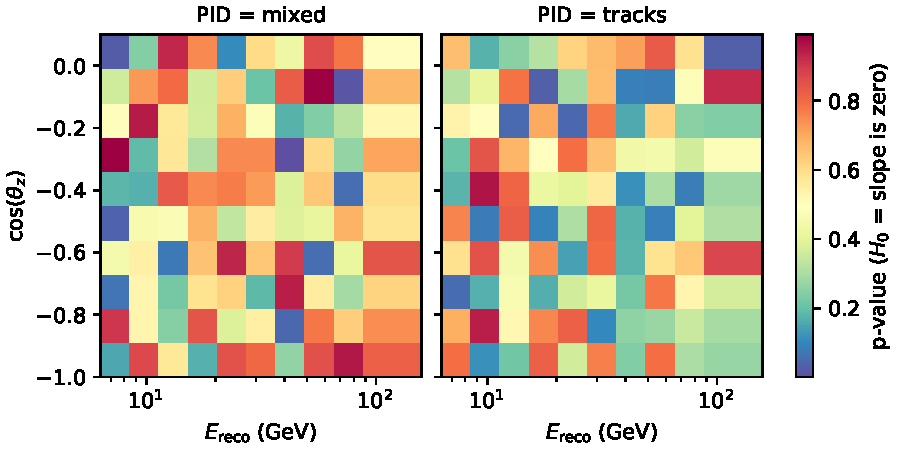
\includegraphics[width=0.9\linewidth]{figures/measurement/systematics/detector/ice_perturbation/steppiness_slope_pvals_verification_sample.pdf}
    \caption{Bin-wise p-value of the fitted slopes as a function of the step-function ice model variation.}
    \label{fig:steppiness-pvals}
\end{figure}

\subsection{Variation of the Atmospheric Neutrino Flux}
\label{sec:flux_systs}

The atmospheric neutrino flux can vary depending on the choice of primary cosmic ray (CR) model, assumed meson yield, hadronic interaction (HI) model and atmospheric density model that are used in the calculation.
The nominal flux, $\Phi_\mathrm{nom}$, is modified to a systematic flux, $\Phi_\mathrm{sys}$, so that

\begin{equation}
    \Phi_{\mathrm{sys}}(E) = \Phi_{\mathrm{nom}} \cdot \left( \frac{E}{E_\mathrm{pivot}}\right)^{\Delta \gamma}
    +
    \sum_{i=1}^{N_\mathrm{Barr}} B_i \cdot \frac{\mathrm{d} \Phi_{\mathrm{nom}}}{\mathrm{d}B_i}\label{eq:flux-variation}
\end{equation}

The $\Delta \gamma$ in \refeq{flux-variation} is due to the CR flux uncertainty and corresponds to shifting the spectral index of the neutrino flux, with a pivot point at $E_\mathrm{pivot}=24\;\mathrm{GeV}$. The second term describes the uncertainty of the Pion and Kaon production yield, where each $B_i$ corresponds to the variation in one \emph{Barr block} (further described below). The gradients with respect to these variations, $\frac{\mathrm{d} \Phi_{\mathrm{nom}}}{\mathrm{d}B_i}$, are calculated using the \textsc{MCEq}\cite{mceq, fedynitch2012influence,fedynitch2015calculation} flux calculator.

\subsubsection{Uncertainty on Meson Production}
\labsec{barr-scheme}
The Barr scheme\sidecite{Barr2006} entails dividing the phase space of incident parent particle $E_\mathrm{i}$ and the outgoing secondary particle $E_\mathrm{s}$ (or, equivalently, $x_{\mathrm{LAB}}=E_\mathrm{s}/E_\mathrm{i}$) into regions that are each denoted by a Barr variable.
There are eight regions/variables that define the uncertainty on $ \pi^+ $ production, and four regions that define the $K^+$ production, as shown in \reffig{barr-blocks}.
For every region, a different relative uncertainty is assigned based on the experimental constraints in that region, as shown in \reffig{barr-blocks-uncertainty}.
For primary particle energies $>500\;\mathrm{GeV}$, an additional energy-dependent term is added to the uncertainty to account for the fact that no accelerator measurements are available at these energies to constrain the meson yield.
As the pion ratio is well-measured, the uncertainty on $ \pi^- $ is defined by the uncertainty on $ \pi^+ $ combined with the uncertainty on the pion ratio.
The uncertainty on $ K^- $ production is parametrized separately from the $K^+$ production.
The only modification to the original Barr scheme used in this analysis is that the low-energy $ \pi^+ $ Barr variables A-F are summarized to a single variable with a relative uncertainty of 63\%, because their impact was found to be highly correlated.
Thus the uncertainty from meson production is described by $N_\mathrm{Barr}=17$ Barr variables that enter \refeq{flux-variation}.

\begin{figure}
    \centering
    \tikzsetnextfilename{barr_blocks_annotated}%
\begin{tikzpicture}
    \node[above right, inner sep=0] (image) at (0,0) {
        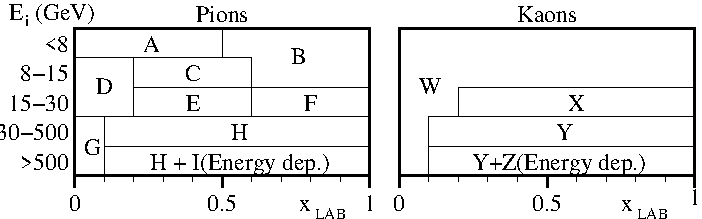
\includegraphics[width=0.8\linewidth]{figures/measurement/systematics/flux/barr_blocks.pdf}
    };
    % Create scope where axes are matching the Pion grid
    \begin{scope}[
        x={($0.42*(image.south east)$)},
        y={($0.67*(image.north west)$)},
        shift={($0.107*(image.south east) + 0.2*(image.north west)$)}
    ]
        % Grid
        %\draw[darkgray,step=0.2] (0,0) grid (1,1);
        \draw[thick, orange, fill=orange, fill opacity=0.8] (0, 0.4) rectangle (1, 1);
        \node[anchor=south, fill=white, draw=black] at (0.5, 0.55) {merged A-F};
    \end{scope}
\end{tikzpicture}
    %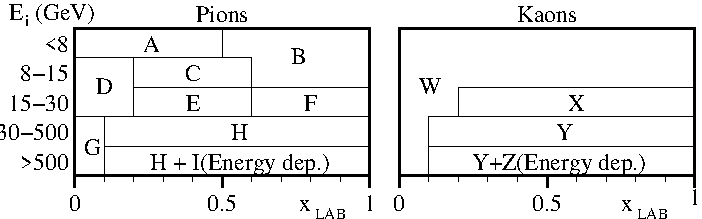
\includegraphics[width=0.8\linewidth]{figures/measurement/systematics/flux/barr_blocks.pdf}
    \caption{Fully correlated regions of uncertainties in the hadronic interaction model. Figure taken from \cite{Barr2006}.}
    \labfig{barr-blocks}
\end{figure}
\begin{figure}
    \centering
    \tikzsetnextfilename{barr_blocks_uncertainty_annotated}%
\begin{tikzpicture}
    \node[above right, inner sep=0] (image) at (0,0) {
        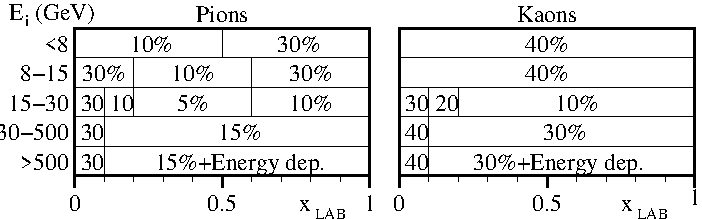
\includegraphics[width=0.8\linewidth]{figures/measurement/systematics/flux/barr_blocks_uncertainty.pdf}
    };
    % Create scope where axes are matching the Pion grid
    \begin{scope}[
        x={($0.42*(image.south east)$)},
        y={($0.67*(image.north west)$)},
        shift={($0.107*(image.south east) + 0.2*(image.north west)$)}
    ]
        % Grid
        %\draw[darkgray,step=0.2] (0,0) grid (1,1);
        \draw[thick, orange, fill=orange, fill opacity=0.8] (0, 0.4) rectangle (1, 1);
        \node[anchor=south, fill=white, draw=black] at (0.5, 0.55) {63\%};
    \end{scope}
\end{tikzpicture}
    %\includegraphics[width=0.8\linewidth]{figures/measurement/systematics/flux/barr_blocks_uncertainty.pdf}
    \caption{Relative uncertainty assigned to each region of hadron phase space in percent. Figure taken from \cite{Barr2006}.}
    \labfig{barr-blocks-uncertainty}
\end{figure}

%Only in the sterile analysis, the prior on the variables with an energy-dependent uncertainty, \texttt{barr\_i\_Pi}, \texttt{barr\_z\_K}, and \texttt{barr\_z\_antiK} by a factor of 5 to 0.61, because it was found that the original priors used in the standard three-flavor analysis greatly under-estimated the impact of these parameters compared to the original Barr 2006 paper.

\subsubsection{Atmospheric density}

The development of particle showers in the atmosphere is governed by competing processes of decay and interactions with the surrounding air.
The density of the atmosphere can therefore influence the rate of neutrino production and could potentially contribute a systematic uncertainty to oscillation measurements.
The size of the effect of atmospheric density uncertainty on the analysis presented in this work is estimated using the same procedure as described in \cite{MEOWS}.
This is done by obtaining a variation of atmospheric density profile by perturbing the Earth’s atmospheric temperature within a prior range given by the NASA Atmospheric InfraRed Sounder (AIRS) satellite~\cite{AIRS} temperature data.
The resulting atmospheric density profile are injected into \textsc{MCEq} to calculate new fluxes.
This is performed for a variety of CR models and hadronic interaction models available in \textsc{MCEq}.
The resulting fluctuations of the neutrino flux observed at the detector were found to be consistently below 1\% for the energy ranges most relevant to DeepCore measurements and is therefore not included as a systematic uncertainty in this work.



% Measurement of neutrino oscillation parameters
\setchapterstyle{kao}
\chapter{Three-flavor oscillation measurement}
\setchapterpreamble[u]{\margintoc}
\labch{measurement-three-flavor}

The first measurement made using the data sample described in this work is the measurement of the atmospheric mixing angle $\theta_{23}$ and the mass splitting $\Delta m^2_{32}$.
The experimental setup of DeepCore is ideally suited for this measurement, because the first valley of maximum disappearance for muon neutrinos passing through the entire diameter of the Earth is expected to lie between 20~GeV and 30~GeV as shown in \reffig{three-flavor-oscprob} in \refsec{atmospheric-neutrino-oscillations}.
The parameter $\Delta m^2_{32}$ changes the position of the oscillation valley in energy, while $\theta_{23}$ changes its amplitude.
In the analysis histogram, this muon neutrino disappearance effect is evident even by just a look in the PID channel for highly track-like events, as shown in \reffig{nominal-hist-null-hypo}.
For this measurement, oscillation probabilities are calculated in the three-flavor oscillation scheme including matter effects.
The matter profile of Earth is modeled as concentric shells of a constant density following the Preliminary Reference Earth Model (PREM)\sidecite{PREM}.
The Monte-Carlo simulated events are weighted in a staged procedure where each stage updates the event weights according to flux, cross-sections and oscillation probabilities\sidecite{PISA}.
The oscillation probabilities are calculated using a \textsc{Python} implementation of the Barger~et~al.\sidecite{barger-oscillations} calculation.

%\begin{figure}
%    \centering
%    %\includegraphics[width=0.9\linewidth]{figures/measurement/three_flavor/numu_surv_prob_no_sterile_no_text.png}
%    \tikzsetnextfilename{numu_surv_prob_no_sterile}%
\begin{tikzpicture}

\definecolor{darkgray176}{RGB}{176,176,176}

\begin{axis}[
    % it is important to set this option only for the axis, not for the entire plot!
    % Otherwise, the label of the colorbar will be cut off... 
    set layers=axis on top,
    colorbar,
    colorbar style={
        ylabel={$P(\nu_\mu\rightarrow\nu_\mu)$},
        tick pos=right,
        ytick style={color=black},
        tick align=outside
    },
    colormap={mymap}{[1pt]
      rgb(0pt)=(0.368627450980392,0.309803921568627,0.635294117647059);
      rgb(1pt)=(0.196078431372549,0.533333333333333,0.741176470588235);
      rgb(2pt)=(0.4,0.76078431372549,0.647058823529412);
      rgb(3pt)=(0.670588235294118,0.866666666666667,0.643137254901961);
      rgb(4pt)=(0.901960784313726,0.96078431372549,0.596078431372549);
      rgb(5pt)=(1,1,0.749019607843137);
      rgb(6pt)=(0.996078431372549,0.87843137254902,0.545098039215686);
      rgb(7pt)=(0.992156862745098,0.682352941176471,0.380392156862745);
      rgb(8pt)=(0.956862745098039,0.427450980392157,0.262745098039216);
      rgb(9pt)=(0.835294117647059,0.243137254901961,0.309803921568627);
      rgb(10pt)=(0.619607843137255,0.00392156862745098,0.258823529411765)
    },
    log basis x={10},
    point meta max=1,
    point meta min=0,
    tick align=outside,
    tick pos=left,
    x grid style={darkgray176},
    xlabel={energy (GeV)},
    xmin=5, xmax=500,
    xmode=log,
    xtick style={color=black},
    y grid style={darkgray176},
    ylabel={\(\displaystyle \cos(\theta_{\mathrm{z}})\)},
    ymin=-1, ymax=0,
    ytick style={color=black}
]
\addplot graphics [includegraphics cmd=\pgfimage,xmin=5, xmax=500, ymin=-1, ymax=0] {figures/measurement/three_flavor/oscillograms/numu_surv_prob_no_sterile-000.png};
\end{axis}

\end{tikzpicture}

%    \caption{Muon-neutrino survival probability calculated at \textsc{NuFit~4.0}\cite{nufit40} global best fit parameters.}
%    \label{fig:three-flavor-oscprob}
%\end{figure}

\section{Statistical Analysis}

\subsection{Definition of test statistic}
\label{sec:test-statistic}

To make a measurement, the discrepancy between the histograms of the weighted MC events and the observed data events has to be measured by an appropriate test statistic.
This measurement uses a modified $\chi^2$ test statistic defined as
\begin{equation}
\chi^2_{\mathrm{mod}} = \sum_{i \in \mathrm{bins}}^{}\frac{(N^{\nu}_i + N^{\mu}_i - N^{\mathrm{obs}}_i)^2}{N^{\nu}_i + N^{\mu}_i + (\sigma^{\nu}_i)^2 + (\sigma^{\mu}_i)^2} + \sum_{j \in \mathrm{syst}}^{}\frac{(s_j - \hat{s_j})^2}{\sigma^2_{s_j}},
\label{eq:mod-chi2}
\end{equation}
\noindent where $N^{\nu}_i$ and $N^{\mu}_i$ are the expectation values for neutrinos and atmospheric muons, respectively, and $N^{\mathrm{obs}}_i$ is the number of observed events. The expectation value for neutrinos within a bin is calculated as the sum of the neutrino MC event weights $N^{\nu}_i = \sum_{i}^{\nu\,\mathrm{evts}} w_i$, with the statistical uncertainty due to finite simulation statistics $(\sigma^{\nu}_i)^2 = \sum_{i}^{\mathrm{evts}} w_i^2$.
The expectation value for muons, $N^{\mu}_i$, is taken from the KDE-smoothed template shown in \reffig{muon-kde-smoothing}.
The variance of the KDE estimate, $(\sigma^{\mu}_i)^2$, is calculated from a heuristic described below.
The error term due to Poisson fluctuations of the data is calculated with the total MC expectation for muons and neutrinos.
The second term in equation~\ref{eq:mod-chi2} is included as a penalty term to account for prior knowledge of some systematic parameters.

\subsubsection{Muon KDE error estimates}
\label{sec:muon-kde-error-three-flav}
For the three-flavor oscillation analysis, the variance of the muon KDE estimate is calculated using a heuristic based on the theoretical upper bound of the variance of a KDE estimate with a fixed kernel.
If the KDE estimate of the density at the point $x_0$ given $n$ i.i.d.
samples from the true PDF $p$ is $\hat{p}_n(x_0)$, the upper bound on the variance is
\begin{equation}
    \mathrm{Var}(\hat{p}_n(x_0)) \leq \frac{1}{nh}p(x_0)\sigma_K^2\;,\label{eq:kde-var-upper-bound}
\end{equation}
where $h$ is the bandwidth and $\sigma_K^2=\int K^2(y)\,\mathrm{d}y$ with $K$ being the kernel function\sidecite{KDE}.
The true PDF can be approximated with the estimated PDF to obtain an approximate error estimate.
However, the KDE implementation used in this analysis uses a dynamic bandwidth and does not readily give access to $\sigma_K^2$ either.
For this reason, an ad hoc heuristic is used following
\begin{equation}
    (\sigma^{\mu}_i)^2 = \mathrm{Var}(\hat{p}_n(x_0))\approx C\frac{\hat{p}_n(x_0)}{n}\;,\label{eq:kde-var-ad-hoc}
\end{equation}
where $C$ is an overall scaling factor that has to be tuned ''by hand''.
To do this, a least-squares fit is run on the systematic MC sets and the value of $C$ is chosen such that the average $\chi^2/\mathrm{dof}$ from the least-squares fits over all bins is $\approx 1$ when $n$ is the number \emph{unweighted} events in the muon MC sample.
This heuristic encodes the fact that the variance of the KDE estimate should be proportional to the density and inversely proportional to the number of MC events, where the proportionality factor is tuned to the statistical fluctuations between independent MC sets.

\subsection{Modeling of Detector Response}
\label{sec:hypersurfaces}

\begin{marginfigure}[\baselineskip]
    \includegraphics[width=\linewidth]{figures/measurement/systematics/detector/hypersurface_example_v2.png}
    \caption{Example of a linear regression in one bin of the analysis projected onto the dimension of the DOM efficiency. Data points with translucent error bars originate from MC sets where one or more parameters besides DOM efficiency are at off-nominal points and are projected along the fitted surface to the nominal point.}
    \labfig{hypersurface-example-fit}
\end{marginfigure}
For the standard three-flavor fit, the method adopted to model systematic detector uncertainties is an extension to the same method that has been used in previous IceCube oscillation studies\cite{IceCube:2019dqi}.
The expectation value of the analysis histogram is calculated using each of the discrete MC sets with perturbed detector properties, and the expectation values in each bin are divided by the expectation given by the nominal MC set.
Then, a linear least-squares regression is performed for every bin in the histogram to model the expectation value as a function of all five parameters, resulting in five gradients and one intercept value for every bin.
The result of such a fit for an arbitrarily chosen bin is shown in \reffig{hypersurface-example-fit}.
A side effect of this process is that the intercept of the linear regression has a much smaller statistical uncertainty than the statistical uncertainty of the nominal MC set alone, which reduces the statistical MC uncertainty of the analysis overall.

\begin{figure}
    \centering
    \includegraphics[width=0.9\linewidth]{figures/measurement/systematics/detector/hs_grad_dom_eff.pdf}
    \caption{Gradient of the relative bin count with respect to DOM efficiency.}
    \label{fig:dom-efficiency-slopes}
\end{figure}
A fundamental weakness of the linear fit treatment is that the fitted parameters are only valid for the choice of oscillation and flux parameters that they have been fitted with.
In particular, there is a strong interaction between the DOM efficiency parameter and the $\Delta m^2_{31}$ oscillation parameter.
As can be seen in \reffig{dom-efficiency-slopes}, the gradients of the relative bin counts with respect to DOM efficiency show a distinct imprint of the oscillation minimum.
However, the location of this minimum depends on the current value of $\Delta m^2_{31}$, which causes a considerable bias if the value of $\Delta m^2_{31}$ at which the gradients are to be evaluated is different from the value at which they have been fitted.
This is mitigated by running the fits at several values of $\Delta m^2_{31}$ covering the entire plausible range of this parameter, and interpolating all fit parameters with a piece-wise linear function between those points.
As a result, all slopes and intercept values change as a function of the mass splitting.
Although the interactions between detector systematic uncertainties and analysis parameters are not limited to the mass splitting, the bias produced as a result of the choice of other parameters was found to be much smaller and is therefore neglected in the three-flavor analysis.

\subsection{Selection of Free Parameters}
\label{sec:std-osc-free-parameters}

The systematic uncertainties of the oscillation measurement consists of uncertainties on the properties of the detector, the neutrino flux, neutrino cross-sections, and atmospheric muon background.
The effects of each of these uncertainties on the expectation values of the analysis histogram are parametrized by several parameters that are included as nuisance parameters during the fit with Gaussian priors when external constraints are available.
The systematic uncertainties of the detector are described by five parameters, namely DOM efficiency, two hole ice parameters and bulk ice scattering and absorption as described in \refsec{detector-unc}.
Variations of the atmospheric neutrino flux are parametrized by varying the flux contributions of Pions and Kaons in each "Barr block" (see \refsec{flux_systs}) separately.
Neutrino cross-section variations are modeled by varying the axial masses for resonant and quasi-elastic interactions, and by interpolating between the \textsc{GENIE} and \textsc{CSMS} cross-sections for DIS interactions as described in \refsec{xsec_systs}, with an additional 10\% error on the neutral-current contribution to reflect the uncertainty in the hadronization process.
For the atmospheric muon background, both the total normalization and the spectral index of the flux can be varied.

When including all plausible sources of systematic uncertainties described above, the test statistic from \refeq{mod-chi2} would have to be optimized with respect to 28 nuisance parameters. Together with the two physics parameters, this would require an optimization in 30 dimensions to run the analysis. To reduce this computational burden, the potential bias and its significance that could plausibly be produced by each parameter is assessed, and the value of parameters that are found to have a negligible impact is fixed to its global best-fit value. The impact of each parameter is tested as follows: First, pseudo-data \emph{without} statistical fluctuations is produced from simulation where the value of the parameter to be tested is increased by $1\sigma$ if it has a Gaussian prior, or half-way to its upper boundary if it does not have a prior. The histograms are then fit back while keeping the parameter to be tested fixed at its nominal value. This fit is done once with the physics parameters ($\theta_{23}$ and $\Delta m^2_{31}$) fixed at the value that was used to create the pseudo-data, and once with the physics parameters left free. The difference in the test statistic $\chi^2_{\mathrm{mod}}$ between the free fit and the fit with physics parameters fixed to the truth, $\Delta \chi^2_{\mathrm{mod}}$, is referred to as \emph{mis-modeling}.
The p-value of the mis-modeling, calculated under the assumption that it should follow a $\chi^2$-distribution with two degrees of freedom, can be interpreted as the significance with which the analysis would have rejected the true physics value \emph{solely} due to the exclusion of the parameter in question.
This test neglects any global offset to the test statistic, since it would not affect the estimate of the confidence limits for the physics parameters.
\begin{figure}
    \centering
    %\missingfigure[figwidth=0.8\linewidth,figheight=0.7\linewidth]{Mis-modeling grid produced for one parameter in the mis-modeling ranking test.}
    \includegraphics[width=\linewidth]{figures/measurement/three_flavor/asimov_test/systematic_impact_test-asimov_test-000015_GENIE_MA_QE.pdf}
    \caption{Grid of $\Delta \chi^2_{\mathrm{mod}}$ values showing the impact of the axial mass $M_A^{CCQE}$ being pulled by $1\sigma$.}
    \label{fig:systematic-impact-mismod-example}
\end{figure}
The test described above is repeated for a grid of true values of $\theta_{23}$ and $\Delta m^2_{31}$ that span the entire range of values that is not strongly excluded by other measurements, producing a value for $\Delta \chi^2_{\mathrm{mod}}$ at each point in the grid, as shown in \reffig{systematic-impact-mismod-example}. The largest value of $\Delta \chi^2_{\mathrm{mod}}$ of the entire grid produced for one parameter represents the \emph{maximum mis-modeling} for that parameter. Taking the maximum mismodeling for all parameters, one can produce a ranking of the impacts of all parameters of the analysis as shown in \reffig{systematic-impact-mismod-ranking}. Parameters for which the maximum mis-modeling lies below a conservatively chosen value of $\Delta \chi^2_{\mathrm{mod}} < 5\times10^{-3}$ are fixed to their global best-fit value in the analysis, reducing the total number of free parameters to 17.
The complete list of all parameters of the analysis, their priors and their allowed ranges can be found in \reftab{sys-params-three-flavor} in the appendix.
\begin{figure}
    \centering
    %\missingfigure[figwidth=0.6\linewidth, figheight=0.8\linewidth]{Mis-modeling ranking for the three-flavor analysis.}
    \tikzsetnextfilename{three_flavor_mismod_ranking}%
\begin{tikzpicture}
    \begin{semilogxaxis}[
        tick label style = {font=\footnotesize\sffamily},
        xbar,
        xmin=2e-5,
        width=0.9\linewidth,
        height=1.1\linewidth,
        bar width=0.3cm,
        log origin=infty,
        %enlarge y limits=0.5,
        xlabel={maximum $\Delta \chi^2_\mathrm{mod}$},
        symbolic y coords={
            Barr $\bar{K}_\mathrm{Z}$, $\Delta \gamma_\mu$, Barr $\bar{K}_\mathrm{X}$, Barr $K_\mathrm{X}$, Barr $K_\mathrm{Z}$, $\pi^+/\pi^-$ ratio, Barr $\bar{K}_\mathrm{W}$, Barr $\bar{K}_\mathrm{Y}$, Barr $\pi_\mathrm{I}$, Barr $K_\mathrm{W}$, Barr $\pi_\mathrm{G}$, Barr $\pi_\mathrm{H}$, DIS CSMS, GENIE $M_A^{CCQE}$, Barr $\pi_\mathrm{A-F}$, NC norm, Barr $K_\mathrm{Y}$, ice scatter, ice abs, GENIE $M_A^{RES}$, $N_\mu$, $\Delta \gamma_{\nu}$, hole ice $p_1$, hole ice $p_0$, $N_\nu$, $\epsilon_\mathrm{DOM}$
        },
        ytick=data,
        xmajorgrids
    ]
        \addplot table [x=max_mismod, y=param_label, col sep=comma] {
            param_name, param_label, max_mismod
            barr_z_antiK, Barr $\bar{K}_\mathrm{Z}$, 0.0001
            delta_gamma_mu, $\Delta \gamma_\mu$, 0.0001
            barr_x_antiK, Barr $\bar{K}_\mathrm{X}$, 0.0001
            barr_x_K, Barr $K_\mathrm{X}$, 0.0001253586882728502
            barr_z_K, Barr $K_\mathrm{Z}$, 0.0005215688001167906
            pion_ratio, $\pi^+/\pi^-$ ratio, 0.0010014938724447354
            barr_w_antiK, Barr $\bar{K}_\mathrm{W}$, 0.0013617826249995284
            barr_y_antiK, Barr $\bar{K}_\mathrm{Y}$, 0.001784909483961046
            barr_i_Pi, Barr $\pi_\mathrm{I}$, 0.0028407893961021335
            barr_w_K, Barr $K_\mathrm{W}$, 0.009147508698163102
            barr_g_Pi, Barr $\pi_\mathrm{G}$, 0.013435565011888494
            barr_h_Pi, Barr $\pi_\mathrm{H}$, 0.014012540822907371
            dis_csms, DIS CSMS, 0.02336082345524751
            Genie_Ma_QE, GENIE $M_A^{CCQE}$, 0.038519249242069786
            barr_af_Pi, Barr $\pi_\mathrm{A-F}$, 0.04259356987935456
            nu_nc_norm, NC norm, 0.04460453331536404
            barr_y_K, Barr $K_\mathrm{Y}$, 0.06646024427532327
            ice_scatter, ice scatter, 0.0742952038753204
            ice_abs, ice abs, 0.10197443387707672
            Genie_Ma_RES, GENIE $M_A^{RES}$, 0.13818399497979877
            weight_scale, $N_\mu$, 0.4519687304055102
            delta_index, $\Delta \gamma_{\nu}$, 1.4839425295211388
            hole_ice_p1, hole ice $p_1$, 1.7423861973716477
            hole_ice_p0, hole ice $p_0$, 3.1929730025605423
            aeff_scale, $N_\nu$, 4.147319242014547
            dom_eff, $\epsilon_\mathrm{DOM}$, 16.08774037554603
        };
       % the [normalized] keyword is necessary because the axis uses symbolic y coordinates.
       % It is *critical* that there is no space before "[normalized]", and that "axis cs:" 
       % is used explicitly!
        \draw[thick, dashed] (axis cs:5e-3,{[normalized]\pgfkeysvalueof{/pgfplots/ymin}}) -- (axis cs:5e-3,{[normalized]\pgfkeysvalueof{/pgfplots/ymax}});
        \node[draw, thick, single arrow, shape border rotate=180, anchor=east, font=\footnotesize] at (axis cs:5e-3,{[normalized]0}) {fixed};
        \node[draw, thick, single arrow, anchor=west, font=\footnotesize] at (axis cs:5e-3,{[normalized]0}) {free};
    \end{semilogxaxis}
\end{tikzpicture}
    \caption{Ranking of $\Delta \chi^2_{\mathrm{mod}}$ values for all nuisance parameters considered for the three-flavor oscillation analysis.}
    \label{fig:systematic-impact-mismod-ranking}
\end{figure}

\section{Analysis Checks}
Before running the analysis on real data, its robustness is assessed on pseudo-data produced with simulated MC data sets.
Once the robustness on pseudo-data has been established, the analysis is first run \emph{blindly}, that is, without showing the analyzer the results of the physics parameters and only revealing a set of goodness-of-fit variables that has been chosen in advance.
The actual fit values of the measured parameters are only revealed when the values of these variables lie within the plausible range that can be expected from purely statistical fluctuations.

\subsection{Robustness of the minimization}
\label{sec:three-flavor-inject-recover-test}
The free fit of the physics parameters $\theta_{23}$ and $\Delta m^2_{31}$ is run separately once for the lower octant ($\theta_{23} < 45^\circ$) and once for the upper octant ($\theta_{23} > 45^\circ$) to break the degeneracy between the octants. Each fit uses the \textsc{scipy}\cite{2020SciPy-NMeth} implementation of the \textsc{L-BFGS-B} algorithm\cite{l-bfgs-b} to find the parameter values that minimize the $\chi^2_{\mathrm{mod}}$ test statistic.
To ensure that the minimization will always converge to the global optimum for any true value of the physics parameters, pseudo-data without statistical fluctuations (also referred to as an \emph{Asimov} test set) is produced on a grid spanning all values that are not strongly excluded by other experiments and a fit is run for each grid point.
Since there are no statistical fluctuations, the fit is expected to always converge exactly to the injected true value.
As can be seen in the result shown in \reffig{three-flavor-asimov}, the convergence of the minimizer is robust everywhere.
\begin{figure}
    \centering
    \includegraphics[width=0.9\linewidth]{figures/measurement/three_flavor/asimov_test/inject_recover_map.png}
    \caption{Asimov inject/recover test result for the three-flavor oscillation analysis.}
    \label{fig:three-flavor-asimov}
\end{figure}

\subsection{Ensemble tests}
\label{sec:three-flavor-ensemble}
To get expected distributions of the test statistic and parameter fluctuations, the analysis is run on an ensemble of fluctuated pseudodata. For every trial of the ensemble, the expectation value in every analysis bin is first drawn from a normal distribution centered on the MC expectation with a standard deviation corresponding to the MC uncertainty. Using these sampled expectation values, the bin count is drawn from a Poisson distribution independently in every bin. This sampling scheme ensures that the fluctuations reflect both the MC uncertainty and the Poisson fluctuations expected in data. A free fit is run on every trial, producing a set of best-fit parameters, a value for the total $\Delta \chi^2_{\mathrm{mod}}$ test statistic, as well as the chi-square value in each individual bin of the analysis histogram.
%The distribution for the fit parameters and their pull from their injected values from the ensemble is shown in \reffig{three-flavor-ensemble-param}. The distributions for all parameters are centered on the injected value, demonstrating that the fit is behaving robustly under the expected fluctuations.

% \begin{figure}
%     \centering
%     \begin{subfigure}[t]{0.99\textwidth}
%         \centering
%         \includegraphics[width=0.99\textwidth]{figures/measurement/three_flavor/ensemble_pre_fit/ensemble_fitdist.png}
%     \end{subfigure}
%     \begin{subfigure}[t]{0.65\textwidth}
%         \centering
%         \includegraphics[width=0.99\textwidth]{figures/measurement/three_flavor/ensemble_pre_fit/ensemble_pull.png}
%     \end{subfigure}
%   \caption{Distributions of fitted values of each parameter considered in the three-flavor analysis (top), and their corresponding pulls from nominal (bottom).
%   \label{fig:three-flavor-ensemble-param}}
% \end{figure}


\subsubsection{Goodness of Fit}

Before looking at the best fit parameters of the real data fit, the goodness of fit is assessed using the total and bin-wise test statistic distributions.
The distribution of the test statistic acquired from the ensemble described in \refsec{three-flavor-ensemble} is shown in \reffig{three-flavor-ts-ensemble} together with the observed test statistic from real data.
The observed test statistic is found to lie very well within the expectation with a p-value of 32\%.
The bin-wise contribution and the test statistic and its expected distribution are shown in \reffig{three-flavor-binwise-ts}.
The histogram shows no apparent regions of particularly bad agreement between the data and the MC expectation, and the distribution of the bin-wise test statistic is in agreement with the distribution expected from pseudo-data trials.

\begin{figure}
    \centering
    \includegraphics[width=0.8\linewidth]{figures/measurement/three_flavor/ensemble_pre_fit/overall_ts_wings_trials.pdf}
    \caption{Observed test statistic value of the three-flavor oscillation analysis compared to expected distribution from ensemble.}
    \label{fig:three-flavor-ts-ensemble}
\end{figure}

\begin{figure*}
    \centering
    \includegraphics[height=0.22\linewidth,trim={0 0 0 1.5cm},clip]{figures/measurement/three_flavor/ensemble_pre_fit/real_fit_binwise_pulls_pre_bugfix.pdf}
    \includegraphics[height=0.22\linewidth]{figures/measurement/three_flavor/ensemble_pre_fit/binwise_ts_wings_trials.pdf}
    \caption{Contribution of every bin to the over-all test statistic in the three-flavor analysis (left) and their observed distribution compared to the expected distribution from pseudo-data trials (right).}
    \label{fig:three-flavor-binwise-ts}
\end{figure*}

\subsubsection{Test for un-physical mixing}
If the real data contains an under-fluctuation in the oscillation valley, it is possible that the fit prefers more than maximal $\nu_\mu$ disappearance, which is physically not possible.
This tendency to fit unphysical magnitudes of $\nu_\mu$ disappearance is tested by running a fit in which the oscillation probabilities are calculated with a simplified two-flavor model as described in \refsubsec{two-neutrino-mixing}. Rather than parametrizing amplitudes of the flavor transition probabilities by the mixing angle, however, the scale of the oscillation, $\sin^2(2\theta_{23})$, is replaced with a scaling factor that is allowed to float freely even to unphysical values where $\sin^2(2\theta_{23}) > 1$.
If the true mixing angle is $\theta_{23}=45^\circ$, it is expected that such unphysical best-fit values can occur solely due to random Poisson fluctuations of the data.
To quantify this expectation, another ensemble of trials is produced where the injected true mixing is maximal.
The two flavor analysis is run on each trial to produce a distribution of expected values that is shown in \reffig{two-flavor-ensemble}.
The results show that, while the real data fit does indeed prefer a slightly unphysical $\nu_\mu$ disappearance, this preference still lies well within the expectation from random fluctuations if the true mixing was assumed to be maximal.

\begin{figure}
    \centering
    \tikzsetnextfilename{two_flavor_ensemble_threshold_anotated}%
\begin{tikzpicture}
    \node[above right, inner sep=0] (image) at (0,0) {
        \includegraphics[width=0.8\linewidth]{figures/measurement/three_flavor/ensemble_pre_fit/two_flav_ensemble_threshold.png}
    };
    % Create scope where axes are the plot coordinates
    \begin{scope}[
        x={($0.4*(image.south east)$)},
        y={($0.45*(image.north west)$)},
        shift={($0.13*(image.south east) + 0.17*(image.north west)$)}
    ]
        % Grid
        %\draw[darkgray,step=.25] (0,0) grid (2,1.5);
        % x-coordinates start at 0.9 and one unit = 0.1
        \draw (1.23, 0) -- node [sloped, font=\footnotesize, anchor=south] {observed $=1.023$} (1.23, 1.3);
    \end{scope}
\end{tikzpicture}
    %\includegraphics[width=0.8\linewidth]{figures/measurement/three_flavor/ensemble_pre_fit/two_flav_ensemble_threshold.png}
    \caption{Observed best fit values of the two-flavor fit compared to the distribution from pseudo-data trials.}
    \label{fig:two-flavor-ensemble}
\end{figure}

\subsubsection{Seasonal Stability}
As described in \refsec{sample-stability}, each season of IceCube data taking lasts approximately one year and begins with a re-calibration of the DOM response and, usually, a new IceCube software release. In addition to the stability of the distributions of individual variables shown in that section, the fluctuations of the fit results of the analysis are also examined for signs of inter-season variations.

To this end, pseudo-data trials are generated where the simulated live time in each trial is one year and the three-flavor fit is run on every trial. The trials are produced at the best fit point of the all-season fit in a way that does not reveal the values of these parameters to the analyzers and the fit results of each parameter are placed into a histogram. From these histograms, the p-value for the observed variations of the best fit results for the individual seasons around the all-season fit is calculated under the null hypothesis that they are solely attributable to statistical fluctuations of the data.  The test does not show any concerning deviations of any parameter from the all-time best fit result. Heat maps of the associated p-values can be found in \reffig{pval-nuisance-parameter-ensemble} in the appendix.

\section{Results}

To prevent biasing the result due to psychological effects such as the well-known confirmation bias\sidecite{Nickerson1998ConfirmationBA}, the results of the analysis are revealed by scripts of code that only print out goodness-of-fit variables such as the test statistic and the parameter pulls to the console while hiding the physics result from the analyzers.
Only after  establishing a good fit of all parameters without any extraordinary pulls, the code reveals the final physics result and likelihood contours that are discussed in this section.

\subsection{Measured Nuisance Parameter Values}
The results for all nuisance parameters are shown in \reftab{nuisance_params_fittedval}.
The pull values show that all parameters fit comfortably within $1\sigma$ of their defined priors.
This is expected, since the analysis is not itself a statistically powerful measurement of most of the parameters being considered, and therefore the best fit values are pulled towards the center of the prior.
The fit prefers a slightly harder cosmic ray spectrum and a larger muon background than initially expected.
The optical efficiency of the DOMs fits to a slightly larger value than nominal with 106\%, while the ice properties stay very close to their initial values.

%The hole ice parameters prefer less acceptance of photons entering the DOMs directly from below, and the shape of their corresponding acceptance curve is close to the best fit result from LED flasher studies\todo{cite hole ice flasher studies} as shown in \reffig{hole-ice-flasher-comparison-three-flavor}.

\begin{table}
    \centering
    \caption{Fitted values of all nuisance parameters from the all-season three-flavor fit. The pull of the best fit value is shown for parameters with a defined prior.}
    \label{tab:nuisance_params_fittedval}
    \begin{tabular}{clSS} \toprule
        category & Parameter  & {Best Fit Value} &  {Pull ($\sigma$)} \\ \midrule
        \multirow{7}{5em}{$\nu$ flux}& $\Delta \gamma_\nu$ & 0.065 & 0.65 \\
        & Barr $\pi_\mathrm{AF}$ & 0.233  & 0.369 \\
        & Barr $\pi_\mathrm{G}$ & -0.055  & -0.183 \\
        & Barr $\pi_\mathrm{H}$ & -0.0179  & -0.119 \\
        & Barr $K_\mathrm{W}$ & 0.0824  & 0.206 \\
        & Barr $K_\mathrm{Y}$ & 0.106  & 0.355 \\
        & Barr $\bar{K}_\mathrm{W}$ & -0.009  & -0.0224 \\ \midrule
        \multirow{4}{5em}{cross-section}& $M_{A}^{CCQE}$ &  0.0283 & 0.0283 \\
        & $M_{A}^{CCRES}$ & 0.572 & 0.572 \\
        & DIS CSMS & 0.0379  & 0.0379 \\
        & NC norm & 1.13 &  0.633 \\ \midrule
        \multirow{5}{5em}{detector systematics} & $\epsilon_\mathrm{DOM}$ & 1.06  & 0.625 \\
        & hole ice $p_0$ & -0.269  &  \\
        & hole ice $p_1$ & -0.041  &  \\
        & ice absorption & 0.974  &  \\
        & ice scattering & 0.989 &  \\ \midrule
        \multirow{2}{5em}{norm}& $N_\mu$ & 1.39  &  \\
        & $N_\nu$ & 0.824 &  \\
        \bottomrule
    \end{tabular}
\end{table}

The best-fit point of the hole ice parameters $p_0$ and $p_1$ is close to the results of the LED flasher fits shown in \reffig{hole-ice-parametrization}.
The resulting light acceptance curve is shown in \reffig{hole-ice-bfp-comparison} compared to the curves produced by \emph{in-situ} LED calibration studies.
The result of the three-flavor oscillation fit agrees with the LED calibration result in preferring a lower forward acceptance than the baseline hole ice model.
\begin{figure}
    \centering
    \tikzsetnextfilename{hole_ice_best_fit_point_comparison}%
\begin{tikzpicture}

\pgfplotstableread{figures/measurement/systematics/detector/hole_ice/all_acceptance_curves.csv}\acceptancecurves

\begin{axis}[
        width=0.8\linewidth, height=0.5\linewidth,
		xmajorgrids, ymajorgrids,
		xlabel=$\cos(\eta)$, ylabel=relative optical efficiency,
		legend style={at={(0.02,0.95)}, anchor=north west},
        ytick distance=0.2,
	]
    \addplot[black, very thick] table [x=cos_theta, y=bfp_three_flav] \acceptancecurves;
    \addlegendentry{best fit point}

    \addplot[black, thick, dashed] table [x=cos_theta, y=baseline] \acceptancecurves;
    \addlegendentry{baseline}
    
    \addplot[bluishgreen, thick] table [x=cos_theta, y=all] \acceptancecurves;
    \addlegendentry{combined LEDs}
    
    \addplot[bluishgreen, thick, dashed] table [x=cos_theta, y=tilted] \acceptancecurves;
    \addlegendentry{tilted LEDs}

    \addplot[bluishgreen, thick, dotted] table [x=cos_theta, y=horizontal] \acceptancecurves;
    \addlegendentry{horizontal LEDs}
	
\end{axis}
\end{tikzpicture}
    \caption{Angular acceptance curves corresponding to the best fit point of the three flavor and sterile oscillation fits compared to the results of LED flasher calibration studies.}
    \label{fig:hole-ice-bfp-comparison}
\end{figure}


\subsection{Oscillation parameters}
The fitted values for the three-flavor oscillation parameters are
\begin{align*}
    \sin^2\theta_{23} &= 0.507_{-0.053}^{+0.050}\\
    \Delta m^2_{32} &= 2.42_{-0.75}^{+0.77} \times10^{-3}\;\mathrm{eV}^2.
\end{align*}
The 90\% C.L.
allowed region for these parameters is shown in \reffig{real_data_contour_three_flavor} along with measurements from other experiments.
The observed confidence limits for $\theta_{23}$ are slightly smaller than what would be expected from a likelihood scan over Asimov pseudo-data that was produced at the best fit point.
To make sure that this is compatible with random fluctuations, the likelihood is profiled over $\sin^2(\theta_{23})$ for 100 pseudo-data trials including both Gaussian fluctuations that emulate the MC uncertainty and Poisson fluctuation for the data uncertainty.
\reffig{mixing_brazil_band_three_flavor} shows the 68\% (90\%) intervals of the test statistic at each point of the scan over all trials.
The observed contour is fully contained in the 68\% band, demonstrating that the narrowed 90\% range for $\theta_{23}$ is fully compatible with expected data fluctuations.
The contribution of each category of systematic uncertainties shown in \reftab{nuisance_params_fittedval} to the total uncertainty is shown in \reftab{error_budget}.
The values show that the largest contribution to the total systematic uncertainty of the analysis is by far the uncertainty on the detector properties.
Overall, the result provides constraints on the atmospheric mass splitting and mixing angle that are the most stringent in its class of experiments and are competitive with those from accelerator experiments\cite{t2k_neutrino_2020,MINOS:2020llm,NOvA:2021nfi}.
\begin{margintable}
    \caption{Contribution of each category of systematic uncertainties to the total error budget in each physics parameter.}
    \label{tab:error_budget}
    \begin{tabular}{p{4em}SS}
        \toprule
        & \multicolumn{2}{c}{error contrib. (\%)} \\ \cmidrule{2-3}
        category & $\Delta m^{2}_{32}$ & $\sin^{2}\theta_{23}$  \\
        \midrule
        $\mu$ norm       & 1.8   & 1.1    \\
        $\nu$ norm       & 1.0   & 0.4    \\
        detector         & 33.6  & 10.6   \\
        $\nu$ flux       & 5.4   & 1.4    \\
        cross-section    & 6.8   & 0.3    \\
        \bottomrule
    \end{tabular}
\end{margintable}

\begin{figure}
    \centering
    %\includegraphics[width=\textwidth]{figures/measurement/three_flavor/results/real_data_contour.png}
  \tikzsetnextfilename{three_flavor_contour}%
\begin{tikzpicture}

\begin{axis}[
	xmin=0.32, xmax=0.68,
	ymin=1.9e-3, ymax=3.3e-3,
	xmajorgrids, ymajorgrids,
	legend columns=2,
	transpose legend=false,
	xlabel={$\sin^2(\theta_{23})$},
	ylabel={$\Delta m^2_{32}\;(\mathrm{eV^2})$},
	ytick distance=0.2e-3
]

\addplot [orange, thick] table [header=false] {figures/measurement/three_flavor/results/contours/SuperK__sin2_theta23_dm2_32__90pc_2020.csv};
\addlegendentry{SuperK 2020}

\addplot [skyblue, thick, densely dotted] table [header=false] {figures/measurement/three_flavor/results/contours/MINOS_numu_disappearance_90pc_2016.csv};
\addlegendentry{MINOS 2016}

\addplot [bluishgreen, thick, densely dotted] table [header=false] {figures/measurement/three_flavor/results/contours/T2K_sin2_theta23_dm2_32__90pc_2020.csv};
\addlegendentry{T2K 2020}

\addplot [vermilion, thick, densely dotted] table [header=false] {figures/measurement/three_flavor/results/contours/NOvA__sin2_theta23_dm2_32__90pc_2021.csv};
\addlegendentry{NO$\nu$A 2021}

\addplot [black, thick, dashed] table [col sep=comma, header=false] {figures/measurement/three_flavor/results/contours/DeepCore_oscNext_verification_sample__sin2_theta23_dm2_32__90pc_sens_at_bfp_all_syst_bugfix.csv};
\addlegendentry{this work (sensitivity)}

%\addplot [black, thick, dashed] table [col sep=comma, header=false] {figures/measurement/three_flavor/results/contours/DeepCore_oscNext_verification_sample__sin2_theta23_dm2_32__90pc_sens_at_bfp_bugfix.csv};
%\addlegendentry{sensitivity at nominal}

\addplot [black, very thick] table [col sep=comma, header=false] {figures/measurement/three_flavor/results/contours/DeepCore_oscNext_verification_sample__sin2_theta23_dm2_32__90pc_result_bugfix.csv};
\addlegendentry{this work}

% best fit point
\addplot [mark=otimes] coordinates{(0.507, 2.41937e-3)};

\node[plot annotation, text width=3.5 cm, anchor=south west] at (axis description cs:0.01, 0.01) {all contours 90\% C.L.};
% \node[font=\sffamily\footnotesize, red, anchor=south east] at (axis description cs:0.99, 0.01) {\emph{IceCube preliminary}};

\end{axis}

\end{tikzpicture}
  \caption{Contours showing the 90\% C.L.
allowed region for the physics parameters of the three-flavor analysis and of other experiments\cite{SK2020,t2k_neutrino_2020,MINOS:2020llm,NOvA:2021nfi}.
The sensitivity for this work is calculated at the best fit point and the cross shows the best fit value.
Other experiments shown in dotted lines are accelerator results, while solid lines are atmospheric oscillation results.
All contours shown assume Normal Ordering.
  \label{fig:real_data_contour_three_flavor}}
\end{figure}

\begin{figure}
    \centering
    %\includegraphics[width=0.8\textwidth]{figures/measurement/three_flavor/results/mixing_brazil_band.pdf}
    \tikzsetnextfilename{three_flavor_mixing_brazil_band}%
\begin{tikzpicture}
\pgfplotstableread[col sep=comma]{figures/measurement/three_flavor/results/brazil_bands/mixing_brazil_band_data.csv}\table

\pgfplotsset{set layers=axis on top}

% 68% interval: 0.45422922, 0.55732256
% 90% interval: 0.42675708, 0.58344331
% BFP: 0.507

\begin{axis}[
    xmin=0.37, xmax=0.63,
    %xmin=0.32, xmax=0.68,
    ymin=0, ymax=6,
    xmajorgrids,
    %ymajorgrids,
    xlabel={$\sin^2(\theta_{23})$},
    ylabel={$\Delta \chi^2_\mathrm{mod}$},
    ylabel style={at={(-0.1,0.5)}},
    height=0.45\linewidth,
    width=0.8\linewidth,
    % extra x ticks={0.42675708, 0.45422922, 0.55732256, 0.58344331},
    % extra x tick labels={90\% lower, $-1\sigma$, $+1\sigma$, 90\% upper},
    % extra x tick style={grid=major},
    extra y ticks={0.988946481478023, 2.705543454095404},
    extra y tick labels={$1\sigma$, 90\%},
    extra y tick style={grid=major}
    %ytick distance=2
]

\addplot[black, very thick] table [x=sin2_theta23, y=metric_real_data] \table;
\addlegendentry{observed}
\addplot[black, thick, dashed] table [x=sin2_theta23, y=metric_asimov] \table;
\addlegendentry{sensitivity}

%\addplot[blue] table [x=sin2_theta23, y=median_contour] \table;

\addplot[yellow, name path=pct_90_lo, forget plot] table [x=sin2_theta23, y=pct_90_lo] \table;
\addplot[yellow, name path=pct_90_hi, forget plot] table [x=sin2_theta23, y=pct_90_hi] \table;
\addplot[yellow] fill between [of=pct_90_lo and pct_90_hi];
\addlegendentry{90\% band}

\addplot[green, name path=pct_68_lo, forget plot] table [x=sin2_theta23, y=pct_68_lo] \table;
\addplot[green, name path=pct_68_hi, forget plot] table [x=sin2_theta23, y=pct_68_hi] \table;
\addplot[green] fill between [of=pct_68_lo and pct_68_hi];
\addlegendentry{68\% band}

\end{axis}
\end{tikzpicture}

    \caption{Observed contour in $\sin^2(\theta_{23})$ (solid) compared to the Asimov expectation (dashed) and the distribution of 100 pseudo-data trials (yellow and green bands) produced at the best fit point of the three-flavor oscillation analysis.
The observed contour is fully contained within 68\% of the fluctuations of the trials.
  \label{fig:mixing_brazil_band_three_flavor}}
\end{figure}

\subsection{Post-fit Data/MC agreement}

Using the weights of the MC events at the best fit point, the post-fit agreement between data and simulation can be shown for any variable.
Of particular interest is the distribution of the argument to neutrino oscillations, $L/E$, where $L$ is the total distance traveled by a neutrino and $E$ is its energy.
Although the true value of the oscillation argument is unknown for data events, it can nevertheless be calculated from the reconstructed energy and zenith angle.
The resulting distribution is shown in \reffig{data_mc_post_fit_l_over_e} and displays a good agreement between data and simulation, with a reduced $\chi^2$ of close to unity.
The comparison between data and simulation for the reconstructed zenith angle and energy gives reduced $\chi^2$ values of 0.782 and 1.19, respectively, when calculated in the same binning.

% \begin{figure*}
%     \centering
%     \ref{reco_coszen_postfit_threeflav_legend}\par
%     \tikzsetnextfilename{final_level_postfit_three_flav_reco_coszen}%
\begin{tikzpicture}
    \pgfplotstableread{figures/measurement/three_flavor/results/data_mc_post_fit/reco_coszen.csv}\table
    \begin{groupplot}[
        xmin=-1.055,xmax=0.15500000000000003,
        xmode=normal,
        xmajorgrids, ymajorgrids,
        width=0.45\linewidth,
        ylabel style={at={(-0.15,0.5)}},
        group/.cd,
        group size=1 by 2,
        xticklabels at=edge bottom,
        vertical sep=10pt
        ]
    \nextgroupplot[
        height=0.3\linewidth,
        legend cell align={left},
        legend columns=-1,
        legend to name=reco_coszen_postfit_threeflav_legend,
        ymode=log,
        ymin=3e-8, ymax=3e-5,
        ylabel=rate (Hz),
        % add magic filter to correctly handle empty bins in logarithmic y-axes:
        % If a bin-count is too low or zero, it would cause the line to be
        % interrupted, which creates artefacts and ugliness. Instead, we replace
        % these bin-counts with values that are just below the axis limit.
        % Because of the way pgfplots works, the input is the raw number but the
        % output has to be the log. Weird, I know.
        % y filter/.expression={y < 4.228878698498991e-09 ? ln(4.2288786984989913e-10) : ln(y)}
        y filter/.expression={y < \pgfkeysvalueof{/pgfplots/ymin} ? ln(\pgfkeysvalueof{/pgfplots/ymin}) - 1 : ln(y)}
    ]

    \ploterrorband[muon_color]{muon}{1}
    \addlegendentry{atm. muons}

    \ploterrorband[nue_color]{nuenuebar}{1}
    \addlegendentry{$\nu_e + \bar{\nu}_e$}

    \ploterrorband[numu_color]{numunumubar}{1}
    \addlegendentry{$\nu_\mu + \bar{\nu}_\mu$}

    \ploterrorband[nutau_color]{nutaunutaubar}{1}
    \addlegendentry{$\nu_\tau + \bar{\nu}_\tau$}


    % alternative event breakdown by interaction
    % \ploterrorband[nue_color]{nue_ccnuebar_cc}{1}
    % \addlegendentry{$\nu_e + \bar{\nu}_e$, CC}
    %
    % \ploterrorband[numu_color]{numu_ccnumubar_cc}{1}
    % \addlegendentry{$\nu_\mu + \bar{\nu}_\mu$, CC}
    %
    % \ploterrorband[nutau_color]{nutau_ccnutaubar_cc}{1}
    % \addlegendentry{$\nu_\tau + \bar{\nu}_\tau$, CC}
    %
    % \ploterrorband[nc_color]{nuall_ncnuallbar_nc}{1}
    % \addlegendentry{all $\nu$, NC}

    \ploterrorband{total_mc}{1}
    \addlegendentry{total MC}

    \ploterrorbar{data}
    \addlegendentry{data}


    \nextgroupplot[
        height=0.2\linewidth,
        ymin=0.7, ymax=1.3,
        ylabel=rate/total MC,
        xlabel=reconstructed $\cos(\theta_{\mathrm{zenith}})$
    ]

    \ploterrorbar{data_mc_ratio}
    % \plotratioerrorband[muon_color]{muon}{total_mc}
    % \plotratioerrorband[nue_color]{nuenuebar}{total_mc}
    % \plotratioerrorband[numu_color]{numunumubar}{total_mc}
    % \plotratioerrorband[nutau_color]{nutaunutaubar}{total_mc}

    \node[anchor=south, font=\footnotesize] at (axis description cs:0.5, 0.01) {$\chi^2_{\mathrm{mod}}/\mathrm{dof} = 0.782$};
    \end{groupplot}
\end{tikzpicture}

%     \tikzsetnextfilename{final_level_postfit_three_flav_reco_energy}%
\begin{tikzpicture}
    \pgfplotstableread{figures/measurement/three_flavor/results/data_mc_post_fit/reco_energy.csv}\table
    \begin{groupplot}[
        xmin=5.362591587787688,xmax=185.61920737481475,
        xmode=log,
        xmajorgrids, ymajorgrids,
        width=0.45\linewidth,
        ylabel style={at={(-0.15,0.5)}},
        group/.cd,
        group size=1 by 2,
        xticklabels at=edge bottom,
        vertical sep=10pt
        ]
    \nextgroupplot[
        height=0.3\linewidth,
        legend cell align={left},
        legend columns=3,
        legend to name=reco_energy_postfit_threeflav_legend,
        ymode=log,
        ymin=3e-8, ymax=3e-5,
        ylabel=rate (Hz),
        % add magic filter to correctly handle empty bins in logarithmic y-axes:
        % If a bin-count is too low or zero, it would cause the line to be
        % interrupted, which creates artefacts and ugliness. Instead, we replace
        % these bin-counts with values that are just below the axis limit.
        % Because of the way pgfplots works, the input is the raw number but the
        % output has to be the log. Weird, I know.
        % y filter/.expression={y < 1.129498430227963e-09 ? ln(1.1294984302279631e-10) : ln(y)}
        y filter/.expression={y < \pgfkeysvalueof{/pgfplots/ymin} ? ln(\pgfkeysvalueof{/pgfplots/ymin}) - 1 : ln(y)}
    ]

    \ploterrorband[muon_color]{muon}{1}
    \addlegendentry{atm. muons}

    \ploterrorband[nue_color]{nuenuebar}{1}
    \addlegendentry{$\nu_e + \bar{\nu}_e$}

    \ploterrorband[numu_color]{numunumubar}{1}
    \addlegendentry{$\nu_\mu + \bar{\nu}_\mu$}

    \ploterrorband[nutau_color]{nutaunutaubar}{1}
    \addlegendentry{$\nu_\tau + \bar{\nu}_\tau$}


    % alternative event breakdown by interaction
    % \ploterrorband[nue_color]{nue_ccnuebar_cc}{1}
    % \addlegendentry{$\nu_e + \bar{\nu}_e$, CC}
    %
    % \ploterrorband[numu_color]{numu_ccnumubar_cc}{1}
    % \addlegendentry{$\nu_\mu + \bar{\nu}_\mu$, CC}
    %
    % \ploterrorband[nutau_color]{nutau_ccnutaubar_cc}{1}
    % \addlegendentry{$\nu_\tau + \bar{\nu}_\tau$, CC}
    %
    % \ploterrorband[nc_color]{nuall_ncnuallbar_nc}{1}
    % \addlegendentry{all $\nu$, NC}

    \ploterrorband{total_mc}{1}
    \addlegendentry{total MC}

    \ploterrorbar{data}
    \addlegendentry{data}


    \nextgroupplot[
        height=0.2\linewidth,
        ymin=0.7, ymax=1.3,
        ylabel=rate/total MC,
        xlabel=reconstructed energy (GeV)
    ]

    \ploterrorbar{data_mc_ratio}
    % \plotratioerrorband[muon_color]{muon}{total_mc}
    % \plotratioerrorband[nue_color]{nuenuebar}{total_mc}
    % \plotratioerrorband[numu_color]{numunumubar}{total_mc}
    % \plotratioerrorband[nutau_color]{nutaunutaubar}{total_mc}

    \node[anchor=south, font=\footnotesize] at (axis description cs:0.5, 0.01) {$\chi^2_{\mathrm{mod}}/\mathrm{dof} = 1.19$};
    \end{groupplot}
\end{tikzpicture}

%     \caption{Distributions of reconstructed energy and zenith angle at the best fit point of the three-flavor analysis.}
%     \label{fig:post-fit-threeflav-energy-coszen}
% \end{figure*}

\begin{figure}
    \centering
    \tikzsetnextfilename{final_level_postfit_three_flav_l_over_e}%
\begin{tikzpicture}
    \pgfplotstableread{figures/measurement/three_flavor/results/data_mc_post_fit/l_over_e.csv}\table
    \begin{groupplot}[
        xmin=7.6727049901092546,xmax=2606.642641126127,
        xmode=log,
        xmajorgrids, ymajorgrids,
        width=0.8\linewidth,
        ylabel style={at={(-0.15,0.5)}},
        group/.cd,
        group size=1 by 2,
        xticklabels at=edge bottom,
        vertical sep=10pt
        ]
    \nextgroupplot[
        height=0.5\linewidth,
        legend cell align={left},
        legend columns=3,
        ymode=log,
        ymin=3e-8, ymax=8e-5,
        ylabel=rate (Hz),
        % add magic filter to correctly handle empty bins in logarithmic y-axes:
        % If a bin-count is too low or zero, it would cause the line to be
        % interrupted, which creates artefacts and ugliness. Instead, we replace
        % these bin-counts with values that are just below the axis limit.
        % Because of the way pgfplots works, the input is the raw number but the
        % output has to be the log. Weird, I know.
        y filter/.expression={y < \pgfkeysvalueof{/pgfplots/ymin} ? ln(\pgfkeysvalueof{/pgfplots/ymin}) - 1 : ln(y)}
    ]

    \ploterrorband[muon_color]{muon}{1}
    \addlegendentry{atm. muons}

    \ploterrorband[nue_color]{nuenuebar}{1}
    \addlegendentry{$\nu_e + \bar{\nu}_e$}

    \ploterrorband[numu_color]{numunumubar}{1}
    \addlegendentry{$\nu_\mu + \bar{\nu}_\mu$}

    \ploterrorband[nutau_color]{nutaunutaubar}{1}
    \addlegendentry{$\nu_\tau + \bar{\nu}_\tau$}


    % alternative event breakdown by interaction
    % \ploterrorband[nue_color]{nue_ccnuebar_cc}{1}
    % \addlegendentry{$\nu_e + \bar{\nu}_e$, CC}
    %
    % \ploterrorband[numu_color]{numu_ccnumubar_cc}{1}
    % \addlegendentry{$\nu_\mu + \bar{\nu}_\mu$, CC}
    %
    % \ploterrorband[nutau_color]{nutau_ccnutaubar_cc}{1}
    % \addlegendentry{$\nu_\tau + \bar{\nu}_\tau$, CC}
    %
    % \ploterrorband[nc_color]{nuall_ncnuallbar_nc}{1}
    % \addlegendentry{all $\nu$, NC}

    \ploterrorband{total_mc}{1}
    \addlegendentry{total MC}

    \ploterrorbar{data}
    \addlegendentry{data}


    \nextgroupplot[
        height=0.30\linewidth,
        ymin=0.7, ymax=1.3,
        ylabel=rate/total MC,
        xlabel=L/E (km/GeV)
    ]

    \ploterrorbar{data_mc_ratio}
    % \plotratioerrorband[muon_color]{muon}{total_mc}
    % \plotratioerrorband[nue_color]{nuenuebar}{total_mc}
    % \plotratioerrorband[numu_color]{numunumubar}{total_mc}
    % \plotratioerrorband[nutau_color]{nutaunutaubar}{total_mc}

    \node[anchor=south, font=\footnotesize] at (axis description cs:0.5, 0.01) {$\chi^2_{\mathrm{mod}}/\mathrm{dof} = 0.986$};
    \end{groupplot}
\end{tikzpicture}

    \caption{Oscillation argument $L/E$ calculated from reconstructed quantities at the best fit point of the three-flavor oscillation analysis.}
    \label{fig:data_mc_post_fit_l_over_e}
\end{figure}

\subsection{Likelihood Coverage Test}

When drawing the 90\% exclusion contour for the oscillation parameters shown in \reffig{real_data_contour_three_flavor}, it is assumed that Wilks' theorem\sidecite{10.1214/aoms/1177732360} holds, that is, the distribution of the test statistic follows a $\chi^2$ distribution with two degrees of freedom. If more than 90\% of repeated measurements fall below the 90\% threshold, the likelihood is said to be \emph{over-covering}. In the reverse case where fewer than 90\% of repeated measurements fall below the 90\% threshold, the likelihood is said to be \emph{under-covering}. The coverage of the likelihood may change depending on the assumed true parameter values. For this measurement in particular, it is expected that the likelihood should over-cover near maximal mixing, because the mixing angle can no longer provide a full degree of freedom. To test the coverage for particular values of $\theta_{23}$ and $\Delta m^2_{31}$, pseudo-data is generated where these values are injected as true values. The bin counts of the pseudo-data are Poisson-fluctuated to create an ensemble of trials. Then, one free fit is run and another fit where the physics parameters are fixed to their true values. The coverage is then evaluated by counting the fraction of trials for which $\Delta \chi^2_{\mathrm{mod}}$ between these two fits is smaller than the 90\% threshold given by Wilks' theorem.
The results are shown in \reffig{three-flavor-coverage} for a range of points in mixing angle and mass splitting.
As expected, the likelihood is over-covering near maximal mixing, while there is very little dependence of the coverage on the mass splitting.
The likelihood is over-covering for all points in mass splitting in the right panel of \reffig{three-flavor-coverage}, because the injected mixing angle was at the best fit point of the analysis, which is very close to maximal.
In conclusion, the 90\% contours shown in \reffig{real_data_contour_three_flavor} are slightly over-conservative in the region close to maximal mixing.

\begin{figure*}
    \centering
    \includegraphics[width=0.45\linewidth]{figures/measurement/three_flavor/coverage_test/coverage_dm_v3.pdf}
    \includegraphics[width=0.45\linewidth]{figures/measurement/three_flavor/coverage_test/coverage_t23_v3.pdf}
    \caption{Fraction of trials below the 90\% threshold expected from Wilks' theorem for a range of points in mass splitting (left) and mixing angle (right).}
    \label{fig:three-flavor-coverage}
\end{figure*}

\setchapterstyle{kao}
\chapter{Search for sterile neutrino mixing}
\setchapterpreamble[u]{\margintoc}
\label{ch:measurement-sterile}

This analysis assumes the extended 3+1 neutrino PMNS framework, with the parameters to be constrained being the oscillation parameters $\theta_{24}$ and $\theta_{34}$.
The three-flavor atmospheric oscillation parameters and the CP-violating phase $\delta_{24}$ are treated as nuisance parameters.
The mass-splitting of the additional mass eigenstate is fixed at $\Delta m^2_{41}=1\;\mathrm{eV^2}$.
Because the oscillations at Earth-scale baselines occur on much smaller energy scales than can be resolved by DeepCore, the analysis effectively becomes indifferent to the magnitude of $\Delta m^2_{41}$ and constrains the values of $\theta_{24}$ and $\theta_{34}$ based on the \emph{averaged} oscillation effect.
As a consequence, the constraints calculated based on the assumption that $\Delta m^2_{41}=1\;\mathrm{eV^2}$ are still valid even if the true mass splitting is much larger.
This holds true up to mass splitting values of about $m^2_{41}\gtrapprox100\;\mathrm{eV^2}$, where the heavy mass eigenstate becomes so much slower than the light eigenstates that it would no longer interfere with them and decohere\cite{atmo_decoherence}.

\section{Atmospheric oscillations in the presence of an eV-scale sterile neutrino}

\subsection{The 3+1 model}
This analysis probes the "3+1" oscillation model, in which a fourth "sterile" (i.e., non-interacting) neutrino flavor eigenstate $\nu_s$ and mass eigenstate $\nu_4$ with mass splitting $\Delta m^2_{41}$ is added to the standard three-flavor model.
The PMNS mixing matrix is extended by a fourth row and column, which is parametrized with additional mixing angles $\theta_{14}$, $\theta_{24}$, $\theta_{34}$ and CP violating phases $\delta_{14}$ and $\delta_{24}$ as
\begin{align*}
    U_{3+1} =&\begin{pmatrix}
    U_{e1}    & U_{e2}    & U_{e3}   &U_{e4}    \\
    U_{\mu1}  & U_{\mu2}  & U_{\mu3} &U_{\mu4}  \\
    U_{\tau1} & U_{\tau2} & U_{\tau3}&U_{\tau4} \\
    U_{s1} & U_{s2} & U_{s3}&U_{s4} \\
    \end{pmatrix}\\
    =&
    R_{34}(\theta_{34})
    \tilde{R}_{24}(\theta_{24}, \delta_{24})
    \tilde{R}_{14}(\theta_{14}, \delta_{14})
    R_{23}(\theta_{23})
    \tilde{R}_{13}(\theta_{13}, \delta_{13})
    R_{12}({\theta_{12})}\;,
\end{align*}
where $R_{kl}$ are rotation matrices.
The goal of this analysis is to constrain the matrix elements $U_{\mu4}$ and $U_{\tau4}$ with magnitude $|U_{\mu4}|^2=\sin^2(\theta_{24})$ and  $|U_{\tau4}|^2=\sin^2(\theta_{34})\cos^2\theta_{24}$, respectively, via the measurement of $\nu_\mu$ disappearance.

In the presence of an eV-scale sterile neutrino, the standard three-flavor oscillation pattern as a function of neutrino energy and zenith angle is distorted and overlaid with a much faster secondary oscillation pattern.
\reffig{numu_survival_1eV2_full_range} shows the muon-neutrino survival probability in the presence of a fourth mass eigenstate with $\Delta m^2_{41}=1\;\mathrm{eV^2}$ and $\theta_{24}=15^\circ$ as a function of the energy and cosine of the zenith angle, where $\cos(\theta_z)=-1$ indicates that the neutrino is coming directly from below and $\cos(\theta_z)=1$ directly from above.
For up-going neutrinos, the oscillation pattern induced by $\Delta m^2_{41}$ is only resolved at energies of $>\mathcal{O}(1\;\mathrm{TeV})$.
Below $\sim$200~GeV, the oscillation length reaches values of as low as $\mathcal{O}(\mathrm{km})$, which makes them unresolvable below the horizon where baselines are of $\mathcal{O}(10000\;\mathrm{km})$.

\subsection{Neutrino production height effects}
Above the horizon, the distance from the upper layers of the atmosphere where the neutrinos are produced to the detector is small enough to create a distinct oscillation pattern for a fixed production height, as can be seen in the left panel of \reffig{numu_survival_1eV2_full_range}.
Because neutrino production heights vary over a range of tens of kilometers, it is necessary to average the oscillation probability over production heights to obtain a more realistic expectation.
This is done analytically in \texttt{nuSQuIDS}\cite{squids, nusquids} by calculating the averaged vacuum oscillation probability over a uniform distribution.
The right panel of \reffig{numu_survival_1eV2_full_range} shows the oscillation probability with production heights averaged between 10~km and 30~km as describe in \refsec{prod-height-avg-nusquids}.
The oscillation pattern above the horizon is no longer clearly resolvable, but an average disappearance effect for neutrino energies below 20~GeV remains.
The uniform distribution that is assumed to calculate the averaged oscillation probabilities is of course not entirely realistic.
For this reason, only events that arrive at most slightly above the horizon ($\cos(\theta_z)<0.1$) are included in this analysis.

\begin{figure}
    \centering
    \tikzsetnextfilename{numu_surv_compare_height_avg}%
\begin{tikzpicture}

\definecolor{darkgray176}{RGB}{176,176,176}

\begin{groupplot}[
    group style={
        group size=2 by 1,
        ylabels at=edge left,
        yticklabels at=edge left,
        horizontal sep=0.5 cm
    },
    log basis x={10},
    tick align=outside,
    tick pos=left,
    xlabel={energy (GeV)},
    xmin=2, xmax=5000,
    xmode=log,
    xtick style={color=black},
    y grid style={darkgray176},
    ylabel={\(\displaystyle \cos(\theta_{\mathrm{z}})\)},
    ymin=-1, ymax=1,
    ytick style={color=black},
    width=0.55\textwidth
]
\nextgroupplot[
    colorbar horizontal,
    colorbar style={
        xlabel={$P(\nu_\mu\rightarrow\nu_\mu)$},
        width=2*\pgfkeysvalueof{/pgfplots/parent axis width} + \pgfkeysvalueof{/pgfplots/group/horizontal sep},
        height=0.35cm,
        anchor=south west,
        at={(0, 1.05)},
        xticklabel pos=upper,
        tick pos=upper
    },
    colormap={mymap}{[1pt]
      rgb(0pt)=(0.368627450980392,0.309803921568627,0.635294117647059);
      rgb(1pt)=(0.196078431372549,0.533333333333333,0.741176470588235);
      rgb(2pt)=(0.4,0.76078431372549,0.647058823529412);
      rgb(3pt)=(0.670588235294118,0.866666666666667,0.643137254901961);
      rgb(4pt)=(0.901960784313726,0.96078431372549,0.596078431372549);
      rgb(5pt)=(1,1,0.749019607843137);
      rgb(6pt)=(0.996078431372549,0.87843137254902,0.545098039215686);
      rgb(7pt)=(0.992156862745098,0.682352941176471,0.380392156862745);
      rgb(8pt)=(0.956862745098039,0.427450980392157,0.262745098039216);
      rgb(9pt)=(0.835294117647059,0.243137254901961,0.309803921568627);
      rgb(10pt)=(0.619607843137255,0.00392156862745098,0.258823529411765)
    },
    point meta max=1,
    point meta min=0,
]
\addplot graphics [includegraphics cmd=\pgfimage,xmin=1, xmax=10000, ymin=-1, ymax=1] {figures/measurement/sterile_analysis/oscillation_signal/numu_surv_sterile_1eV_th24_15deg_noheightfilter-000.png};

\node[plot annotation, anchor=north east] at (axis description cs:0.99, 0.99) {$h_\mathrm{prod}=20\;\mathrm{km}$};

\nextgroupplot
\addplot graphics [includegraphics cmd=\pgfimage,xmin=1, xmax=10000, ymin=-1, ymax=1] {figures/measurement/sterile_analysis/oscillation_signal/numu_surv_sterile_1eV_th24_15deg_withheightfilter-000.png};

\node[plot annotation, anchor=north east] at (axis description cs:0.99, 0.99) {$10\;\mathrm{km} < h_\mathrm{prod} < 30\;\mathrm{km}$};

\end{groupplot}

\end{tikzpicture}

    \caption{Muon neutrino survival probability in the presence of a fourth mass eigenstate with $\Delta m^2_{41}=1\;\mathrm{eV^2}$ and $\theta_{24}=15^\circ$ with a fixed production height of 20~km (left) and with production heights averaged between 10~km and 30~km (right).\label{fig:numu_survival_1eV2_full_range}}
\end{figure}
%\begin{figure*}
%    \centering
%    \includegraphics[width=0.45\linewidth]{figures/measurement/sterile_analysis/physics/dm41_0.5eV2_th24_15deg_no_filter.png}
%    \includegraphics[width=0.45\linewidth]{figures/measurement/sterile_analysis/physics/dm41_0.5eV2_th24_15deg_avg_height_10-30km.png}
%    \caption{Muon neutrino survival probability in the presence of a fourth mass eigenstate with $\Delta m^2_{41}=0.5\;\mathrm{eV^2}$ and $\theta_{24}=15^\circ$ with a fixed production height of 20~km (left) and with production heights averaged between 10~km and 30~km (right).}
%    \label{fig:numu_survival_0.5eV2_full_range}
%\end{figure*}

\subsection{Oscillation signal for large mass splittings}
In the mass-splitting range where $\Delta m_{41}\approx\mathcal{O}(1\,\mathrm{eV^2})$ and in the energy range of the event sample ($<150\;\mathrm{GeV}$), the presence of a sterile neutrino produces rapid oscillations overlaid on the standard three-flavor oscillation pattern as well as distortions to that pattern itself as shown in \reffig{numu_survival_1eV2_analysis_binning_range} for a mixing angle of $\theta_{24}=15^\circ$.
The oscillation frequency in energy is too large to be resolved by DeepCore, but the average effect still allows us to constrain the magnitudes of $U_{\mu4}$ and $U_{\tau4}$.
The precise value of $\Delta m^2_{41}$ has very little influence on the average amplitude of the oscillations and therefore cannot be recovered in this mass splitting regime.
The oscillation averages stay approximately constant up to mass splitting values of well above $100\;\mathrm{eV^2}$ where decoherence effects begin to play a role\cite{atmo_decoherence}.
\begin{figure*}
    \centering
    \includegraphics[width=0.45\linewidth]{figures/measurement/sterile_analysis/physics/dm41_1.0eV2_th24_15deg_avg_height_10-30km_ana_binning_range.png}
    \includegraphics[width=0.45\linewidth]{figures/measurement/sterile_analysis/physics/dm41_0.1eV2_th24_15deg_avg_height_10-30km_ana_binning_range.png}
    \caption{$\nu_{\mu}$ survival probability at $\Delta m^2_{41}=1\;\mathrm{eV^2}$ (left) and at $\Delta m^2_{41}=0.1\;\mathrm{eV^2}$ (right). The mixing angle is $\theta_{24}=15^\circ$ in both cases}
    \label{fig:numu_survival_1eV2_analysis_binning_range}
\end{figure*}

\subsection{Oscillation signal for small mass splittings}
For mass-splitting values of $\Delta m^2_{41}$ well below $1\;\mathrm{eV^2}$, the oscillation pattern is no longer completely averaged out.
The right panel of \reffig{numu_survival_1eV2_analysis_binning_range} shows the muon-neutrino survival probability in the presence of a sterile neutrino state with mass splitting $\Delta m^2_{41}=0.1\;\mathrm{eV^2}$ and mixing angle $\theta_{24}=15^\circ$.
The highest oscillation minimum in energy and cosine of the zenith angle (upper right corner of the figure) is large enough to be resolvable with DeepCore.
This makes it possible in principle to produce constraints of the mixing matrix elements as a function of the mass-splitting $\Delta m^2_{41}$, although this is beyond the scope of the analysis presented in this thesis.
% \begin{figure}
%     \centering
%     \includegraphics[width=0.8\textwidth]{figures/measurement/sterile_analysis/physics/dm41_0.1eV2_th24_15deg_avg_height_10-30km_ana_binning_range.png}
%     \caption{$\nu_{\mu}$ survival probability at $\Delta m^2_{41}=0.1\;\mathrm{eV^2}$ and $\theta_{24}=15^\circ$}
%     \label{fig:numu_survival_0.1eV2_analysis_binning_range}
% \end{figure}

\section{Oscillation Probability Calculation with \textsc{nuSQuIDS}}
\label{sec:nusquids}

This analysis uses as customized version of the neutrino Simple Quantum Integro-Differential Solver (\textsc{nuSQuIDS})\cite{squids, nusquids} package to calculate oscillation probabilities.
The basic principle behind \textsc{nuSQuIDS} is to calculate the state transition probabilities in the Interaction (Dirac) Picture of quantum mechanics, where the Hamiltonian is divided into the time-independent vacuum oscillation part $H_0$ and the time-dependent interaction part $ H_1(t)$:
\begin{equation}
    H(t) = H_0 + H_1(t)
\end{equation}
In this picture, the operators evolve with $ H_0$ as
\begin{equation}
\bar{O}_I(t)=e^{iH_0t}O_Se^{-iH_0t}\,,
\end{equation}
while state densities evolve with the interaction Hamiltonian $ H_1(t)$
\begin{equation}
\partial_t\bar{\rho}_I(t)=-i[\bar{H}_{1, I}(t), \bar{\rho}_I(t)]\,.
\end{equation}

This state evolution is solved by numerical integration in \textsc{nuSQuIDS}, which is computationally expensive.
However, because fast oscillations within $ H_0$ only play a sub-leading role, this difficult calculation does not have to be performed at every point in the analysis space.
It is sufficient to calculate state densities at a selected set of points, referred to as \emph{nodes}, and to then interpolate the densities between them.
The fast oscillations between the \textsc{nuSQuIDS} nodes are recovered when the probabilities for each flavor, $i$, are projected out with the trace operation on the state density with the (time-evolved) projection operator for that state:
\begin{equation}
p_i(t)=\mathrm{Tr}(\underbrace{\bar{\Pi}^{(i)}(t)}_{\mathrm{proj.\,op.}}\bar{\rho}_I(t))
\end{equation}

\subsection{Node placement}
The nodes where the difficult state integration is calculated do not need to be spaced densely enough in the analysis space to resolve the fast oscillations due to sterile neutrinos, but they do need to resolve matter effects. The state densities change most rapidly (as function of energy) for neutrinos that traverse a lot of matter at low energies. Additionally, there is a sharp break at $\cos(\theta_{\mathrm{zenith}})=-0.84$ where neutrinos begin to pass through the core.
For this reason, the \textsc{nuSQuIDS} nodes are concentrated in three places:
\begin{itemize}
    \item the energy region between 2 GeV and 10 GeV
    \item within a small interval around $\cos(\theta_{\mathrm{zenith}})=-0.84$
    \item the region below $\cos(\theta_{\mathrm{zenith}})=-0.84$
\end{itemize}
\reffig{nusquids-nodes} shows the optimized placement of \textsc{nuSQuIDS} nodes as black dots.

\begin{figure}
    \centering
    \includegraphics[width=0.7\textwidth]{figures/measurement/sterile_analysis/nusquids/0.1eV_sterile_only_height_avg_optim_nodes.png}
    \caption{Optimized placement of \textsc{nuSQuIDS} nodes (black dots) with extra dense node spacing in the three critical regions. The injected value for $\Delta m^2_{41}$ is $0.1\;\mathrm{eV^2}$.}
    \label{fig:nusquids-nodes}
\end{figure}

\subsection{Production height averaging}
\label{sec:prod-height-avg-nusquids}
At eV-scale mass splittings, oscillations are fast enough that significant oscillations occur even at 10-km-scale distances.
If the production height is assumed to be fixed at an exact position, a strong oscillation pattern appears above the horizon that could falsely produce a very high sensitivity in the analysis, driven entirely by events above the horizon.
In reality, production heights can vary within the atmosphere, which smears out the oscillations.
For this analysis, an analytical averaging method was implemented in nuSQuIDS that assumes a uniform distribution of propagation distances between two points.
The start and end point depends on the zenith angle and corresponds to the intersection of the neutrino path with a height of 10 km and 30 km, respectively. Because the bulk of events entering the detector from above the horizon are excluded from the analysis, the precise choice of the lower and upper bound of the height averaging is not very consequential. \reffig{averaging-height-effect} shows the pull in units of the standard deviation of the Poisson fluctuations of the data in each bin that would be expected as a consequence of changing the distance over which the production height is averaged from \SI{20}{\kilo\metre} down to \SI{1}{\kilo\metre}. As expected, bins near the horizon are most affected, but even there bin-wise pulls do not rise above $0.05\sigma$.
\begin{figure}
    \centering
    \includegraphics{figures/measurement/sterile_analysis/pull_prod_height_range_1km_vs_20_km_th24_15_deg_th34_15_deg_verification_sample.pdf}
    \caption{Pull introduced into each bin of the analysis histogram when changing the distance over which the production height is averaged from \SI{20}{\kilo\metre} down to \SI{1}{\kilo\metre} at sterile mixing angles of $\theta_{24}=\theta_{34}=\ang{15}$.\label{fig:averaging-height-effect}}
\end{figure}

\subsection{Low-pass filtering}
\label{sec:low-pass-filtering}
The fast oscillations in the presence of sterile neutrinos are filtered with a low-pass filter during both state evolution and the calculation of probabilities.
This step dramatically increases the speed with which oscillation probabilities can be evaluated.

Vacuum oscillations enter the differential equation governing the state evolution via the time evolution of the interaction Hamiltonian $\bar{H}_{1, I}(t)$.
At low energies, they cause tiny but extremely fast oscillations of the time derivative that the numerical integrator has to keep track of by drastically reducing the step size, slowing down the calculation.
To mitigate this problem and increase performance, a low-pass filter is applied when calculating the RHS of the differential equation.

\begin{figure}
    \centering
    \includegraphics[width=0.7\textwidth]{figures/measurement/sterile_analysis/nusquids/Dm41_0.5eV2_th24_15deg_avg_height_10-30km_lp_belowhor.png}
    \caption{Muon neutrino survival probability in the presence of a sterile neutrino after application of both height averaging and low-pass filtering.}
    \label{fig:nusquids-low-pass-filtering}
\end{figure}

In the presence of sterile oscillations, transition probabilities usually have to be calculated for every single simulated event to average them out in the analysis binning.
Because the MC set has millions of events, doing this would be very expensive even when using nuSQuIDs' state interpolation feature.
In this analysis, a low-pass filter as a function of energy is applied when the transition probabilities are projected out from the state densities to average out very fast oscillations.
With this filtering, it is possible to calculate oscillation probabilities on a fine binning with ~20k bins.
One caveat is that this filtering is not appropriate to apply above the horizon because propagation distances there are short enough that oscillation probabilities don't average out completely.
Therefore, it is applied only below the horizon as shown in \reffig{nusquids-low-pass-filtering}.

\subsubsection{Test of Filter Performance}

To ensure that the chosen cut-off points of the low-pass filters do not introduce significant distortions to the oscillation signal, an inject/recover test is performed on a grid in $|U_{\mu 4}|$ and $|U_{\tau 4}|$ where pseudo-data is produced \emph{without} any low-pass filtering and fit back with the filtering enabled. For every grid point, a second fit is run where $\theta_{24}$ and $\theta_{34}$ are fixed to their true injected values. The p-value of the difference in the test statistic between these two fits, $\Delta \chi^2_{\mathrm{mod}}$, can be interpreted as the significance with which the true value of the mixing angles would be rejected solely due to the mismodeling of the true oscillation probabilities. The results of the mixing parameters fit and the corresponding values of $\Delta \chi^2_{\mathrm{mod}}$ are shown in \reffig{asimov-test-sterile-ana}. Assuming that $\Delta \chi^2_{\mathrm{mod}}$ should follow a $\chi^2$ distribution with two degrees of freedom, the significance of the mis-modeling is very small.
The fit errors for small values of $|U_{\mu 4}|$ and $|U_{\tau 4}|$ are insignificant because the likelihood is very flat in this region of the parameter space.
There are a few points for which the fit did not converge to the true global optimum, as indicated by a negative value of $\Delta \chi^2_\mathrm{mod}$, but the likelihood difference from the injected true parameters is also very small in these cases.

\begin{figure*}
    \centering
    \includegraphics[width=0.49\linewidth]{figures/measurement/sterile_analysis/asimov_test/asimov_vs_v12_fit_err.pdf}
    \includegraphics[width=0.49\linewidth]{figures/measurement/sterile_analysis/asimov_test/asimov_vs_v12_mismod.pdf}
    \caption{Results of the inject/recover test (left) and the corresponding mis-modeling values, $\Delta \chi^2_{\mathrm{mod}}$, attributable to low-pass filtering in \textsc{nuSQuIDS} (right). A negative value of $\Delta \chi^2_\mathrm{mod}$ indicates that the fit did not converge to the true global optimum.}
    \label{fig:asimov-test-sterile-ana}
\end{figure*}

\section{Nuisance oscillation parameters}
Besides the physics parameters $\theta_{24}$ and $\theta_{34}$ to be constrained by the analysis (at a fixed sterile mass splitting $\Delta m^2_{14}$), there are 4 additional mixing angles and 3 CP-violating phases in the 3+1 PMNS matrix as well as the mass splittings $\Delta m^2_{12}$ and $\Delta m^2_{13}$ that influence the oscillation probability. The solar and reactor angles $\theta_{12}$ and $\theta_{13}$ as well as the solar mass splitting $\Delta m^2_{12}$ are constrained by other experiments beyond the sensitivity of this analysis and are fixed at their current global best fit point\sidecite{nufit40}. The effect of the standard three-flavor CP violating phase $\delta_{\mathrm{CP}}=\delta_{13}$ is negligible and is fixed to zero.
The mixing angle $\theta_{14}$ and the phase $\delta_{14}$ are also fixed to zero, since recent reactor data constrains $|U_{e4}|^2 = \sin^2(\theta_{14})$ to $\mathcal{O}(10^{-3})$, which is well below the sensitivity of this analysis\sidecite{global_unitarity_Hu}.
The only nuisance parameters that remain free are the standard 3-flavor atmospheric oscillation parameters $\theta_{23}$ and $\Delta m^2_{13}$ as well as the sterile CP-violating phase $\delta_{24}$.
The effect of $\delta_{24}$ is to shift the oscillation pattern of muon neutrinos as shown in \reffig{sterile-cp-phase-effect}.
The effect runs in the opposite direction for \emph{anti}neutrinos.
Because neutrinos and antineutrinos are nearly indistinguishable in DeepCore, the combined effect of $\delta_{24}$ is a smearing of the oscillation minimum.
Additionally, the sign of $\cos(\delta_{24})$ is approximately degenerate with the neutrino mass hierarchy effect.
It is therefore expected that the analysis will produce very similar results for NO and IO when $\delta_{24}$ is free.
\reftab{oscillation-parameters} gives an overview over all oscillation parameters in the 3+1 model and their treatment in this analysis.
\begin{figure}
    \centering
    \includegraphics[width=0.8\textwidth]{figures/measurement/sterile_analysis/physics/oscillation_bands.pdf}
    \caption{Muon neutrino survival probability for a directly up-going neutrino as a function of energy in the presence of sterile neutrinos at different values of the sterile CP violating phase.}
    \label{fig:sterile-cp-phase-effect}
\end{figure}

\begin{table}
    \centering
    \begin{tabular}{@{}cccp{0.35 \linewidth}@{}}\toprule
        \textbf{parameter} & \textbf{nominal value} & \textbf{fixed?} & \textbf{comment} \\
        \midrule
        $\theta_{14}$ & $0^\circ$ & fixed &  Constr. by reactor data \\
        $\theta_{24}$ & -- & free & Physics parameter\\
        $\theta_{34}$ & -- & free & Physics parameter\\
        $\theta_{12}$ & $33.82^\circ$ & fixed & Constrained by reactor and solar data \\
        $\theta_{13}$ & $8.61^\circ$ & fixed & Constrained by reactor and accelerator data \\
        $\theta_{23}$ & $49.6^\circ$ & free & Atm. mixing angle \\
        $\delta_{13}$ & $0^\circ$ & fixed &  Negligible effect \\
        $\delta_{14}$ & $0^\circ$ & fixed &  No effect when $\theta_{14} = 0^\circ$ \\
        $\delta_{24}$ & -- & free & Smears osc. minimum \\
        $\Delta m^2_{21}$ & $7.39\times10^{-5}\;\mathrm{eV^2}$ & fixed & Constrained by reactor and solar data \\
        $\Delta m^2_{31}$ & $2.525\times10^{-3}\;\mathrm{eV^2}$ & free & Atm. mass splitting \\
        $\Delta m^2_{41}$ & $1\;\mathrm{eV^2}$ & fixed & Averaged out above $1\;\mathrm{eV^2}$ \\
        \bottomrule
    \end{tabular}
    \caption{Oscillation parameters of the 3+1 model and their treatment in this analysis.}
    \label{tab:oscillation-parameters}
\end{table}

\section{Statistical Analysis}

\subsection{Signal in Analysis Binning}
The change in bin counts with respect to the nominal expectation for different combinations of sterile mixing angles at $\Delta m^2_{41}=1\;\mathrm{eV^2}$ is shown in \reffig{oscillation-effects-ana-binning}.
Although a pull in only $\theta_{34}$ by $20^\circ$ has only a very small effect (see the middle panels of \reffig{oscillation-effects-ana-binning}), the combination of both angles can greatly amplify the signal.
The CP-violating phase $\delta_{24}$ only plays a role when both angles $\theta_{24}$ and $\theta_{34}$ are non-zero.
The sensitivity of this analysis to $\theta_{34}$ is entirely due to matter effects experienced by neutrinos passing through the dense core of the Earth.

\begin{figure}
    \centering
    \includegraphics[width=0.95\textwidth]{figures/measurement/sterile_analysis/oscillation_signal/pull_theta_combinations_20deg_dcp24.pdf}
    \caption{Signal in the analysis binning produced by different combinations of $\theta_{24}$, $\theta_{34}$, and $\delta_{24}$ as a fraction of the Poisson error in each bin. The mass splitting of the sterile state is $\Delta m^2_{41}=1\;\mathrm{eV^2}$.}
    \label{fig:oscillation-effects-ana-binning}
\end{figure}

\subsection{Definition of test statistic}
\label{sec:test-statistic-sterile}

The histograms of the data and the expected values estimated by MC are compared using the same modified $\chi^2$ likelihood described in \refsec{test-statistic} that is also used for the three-flavor oscillation analysis.

\subsubsection{KDE error estimates}
To estimate the error on the KDE output, 20 bootstrap samples are drawn separately in each PID channel and the KDE is re-evaluated for each trial.
The expectation value and the standard deviation of the expectation in each bin of the histogram are the mean and standard deviation of these samples, respectively.
The samples are always produced with the same initial random seed to ensure that expectations and errors are reproducible.

\subsection{Modeling of detector response}
\label{sec:ultrasurfaces}

 As described in \refsec{hypersurfaces}, the gradients acquired by bin-wise linear regressions in the analysis histogram are only correct for the particular choice of the flux and oscillation parameters at which they have been fitted.
For the three-flavor analysis, this can be mitigated by a piece-wise interpolation of the gradients as a function of the mass splitting $\Delta m^2_{31}$, and the impact of other parameters is small enough that this one-dimensional interpolation is sufficient.
However, for the sterile analysis, several additional oscillation parameters have the potential to substantially change the shape of the oscillation pattern and therefore change the detector response in each bin.
The grid required to apply the interpolation to all potentially relevant parameters would have to have at least five dimensions and the RAM requirement to hold all those parameters would have been prohibitive.
It was therefore deemed necessary to develop an entirely new method for the treatment of detector systematic uncertainties that completely decouples the detector response from flux and oscillation weights, as described in this section.

The goal of this treatment of detector systematic effects is to find reweighting factors for every event in the nominal MC set that correspond to how much more or less likely that particular event would be if the detector properties were different.
These reweighting factors should be independent from any other event weights, especially flux and oscillation weights.
To get an intuition, one may look at an event in which the reconstructed energy is larger than the true energy.
In the case where the DOM efficiency is higher than nominal, the detector observes more light than is expected from the baseline simulation, and it becomes more likely that such an event occurs and it should therefore get more weight.
On the other hand, if the DOM efficiency is smaller, the reconstructed energy will, on average, be biased downwards.
This makes an event with an overestimated energy less likely and it should therefore get a smaller weight.
This relationship will not change depending on the initial flux of the primary neutrino or oscillation effects because the detector reacts only to the final state.

Using the discrete MC sets with different variations of detector parameters, one needs to find the re-weighting factors, $R_{ik}$, for each event in the nominal MC set, $i$, such that re-weighting every event by its weighting factor produces the same distribution in energy, zenith angle and PID as the off-nominal MC set, $k$.
If the true distributions of event parameters in each MC set was known, this weighting factor could be calculated as the ratio
\begin{equation}
    R_{ik} = \frac{P(X_i|\theta_k)}{P(X_i|\theta_{\rm nominal})} \frac{P(\theta_k)}{P(\theta_{\rm nominal})}\;, \label{eq:ratio-likelihood}
\end{equation}
where $\theta_k$ are the detector parameters of the off-nominal MC set, $k$.
The vector $X_i$ contains the true and reconstructed values for energy and zenith angle, as well as the PID of the event.
 The probability distribution $P(X_i|\theta_k)$ is the distribution of the event parameters in MC set $k$, and $\theta_{\rm nominal}$ contains the values of the detector parameters of the nominal MC set.
The second fraction is the ratio of the total normalization of events under different values of the detector parameters.
For example, if an increase in DOM efficiency increases the total number of events by 10\%, then $P(\theta) / P(\theta_\mathrm{nominal}) = 1.1$.

In practice, of course, the probability distributions $P(X_i|\theta_k)$ are unknown, but the factors $R_{ik}$  can still be extracted from the available MC sets.
The first step is to apply Bayes' theorem to \refeq{ratio-likelihood} to express $R_i$ as the ratio of the posterior probability distribution of the detector parameters given the event parameters,
\begin{equation}
    R_{ik} = \frac{P(\theta_k|X_i)}{P(\theta_\mathrm{nominal}|X_i)}\;. \label{eq:ratio-posterior}
\end{equation}
The posterior distributions, $P(\theta_k|X_i)$, can be acquired from a classifier trained to give the posterior probability that an event with parameters $X_i$ belongs to the MC set $k$.
This means that the task of finding the reweighting factors can be translated into a \emph{classification task}.
Such an inference method, where probability distributions are learned as a ratio of posteriors from a classifier, is also known as a \emph{likelihood-free inference} method.

\subsubsection{K-Neighbors method to calculate posteriors}
In principle, any classifier that provides well-calibrated posterior outputs can be plugged into eq.~\ref{eq:ratio-posterior}.
For this analysis, the simple and robust \emph{k-neighbors} method is used.
The K-Neighbors classifier calculates posterior probabilities by finding the set $\mathcal{N}$ of the $N$ nearest neighbors for every event, $i$.
This set is defined as the set of $N$ events with the smallest Euclidean distance in the event parameters $X$.
  Then, the estimate for the posterior for set $k$ is the fraction of the total weight of the neighbors belonging to set $k$,
\begin{equation}
    P(\theta_k|X_i) = \frac{\sum_{j\in{\mathcal{N}\cup k}} w_j }{\sum_{j\in{\mathcal{N}}} w_j}\;. \label{eq:posterior-knn}
\end{equation}
The weights $w_j$ are the weighted effective area that every simulated MC event corresponds to and correct for the different amount of MC that was produced for every systematic MC set.
They do not include neutrino flux or oscillation effects.

While this method is very robust, it is also prone to over-fitting if the number of neighbors is chosen to be too small.
On the other hand, if the number of neighbors is too large, it might blur out important features and under-fit.
An increased number of neighbors also causes a systematic bias in the probability estimate due to the fact that the distribution across the selected neighbors is not perfectly uniform.
This bias is corrected in linear order by reweighting the events in each neighborhood as described in the Appendix~\ref{apx:knn-correction}.
With this bias correction applied, a neighborhood size of 200 per included MC set was found to be a good compromise between bias and overfitting.

\subsubsection{Classification variables}
The input variables passed into the classifier for each event, $X_i$, need to cover all variables that are used in the binning ($E_{\rm reco},\cos(\theta_{\rm reco}),{\rm PID}$) as well as all variables that are used when re-weighting events by flux and oscillation probabilities ($E_{\rm true},\cos(\theta_{\rm true})$)\footnote{Even if other variables can in principle influence the detector response, they do not have to be included as long as their distribution does not change.
See also Appendix \ref{apx:implicit-marginalization}.}.
This gives a total of five input variables that are used for classification.
Because the K-neighbors classifier calculates euclidean distances between events in these five dimensions to determine which events are neighbors, all dimensions are transformed to be approximately normally distributed as follows and then scaled to have a unit variance:
\begin{itemize}
    \item Energies are replaced by their logarithm
    \item The zenith angle is used directly, rather than its cosine
    \item The PID, which is the probability output of a BDT, is transformed into the log-odds ratio, $\mathrm{LOR}=\log({\rm PID}) - \log(1-{\rm PID})$.
This transformed variable turns the pileup of events near a PID value of one into a long tail.
\end{itemize}
The classifier is fit to the transformed variables separately for each flavor for CC interactions and to the combined set of all NC interactions.

\subsubsection{Calculating event-wise gradients}

The K-Neighbors calculation produces event weights that can reweight the events of the nominal MC set to imitate the distribution of any other MC set.
To be useful in an analysis, however, it is a requirement that this re-weighting can be interpolated to any value of detector parameters between the discrete MC sets.
This is accomplished by fitting a vector of gradients, $g_i$, for every event, minimizing the negative log-likelihood
\begin{equation}
    -\log\mathcal{L} = -\sum_k P_{\rm obs}(\theta_k | X_i) \log P_{k, \rm pred}(g_i, X_i)\;, \label{eq:grad-nllh}
\end{equation}
where the observed probability is $P_{\rm obs}(\theta_k | X_i)$ from the K-neighbors calculation and the  predicted probability $P_{k, \rm pred}(g_i, X_i)$ is
\begin{equation}
    P_{k, \rm pred}(g_i, X_i) = \frac{\exp(\sum_j \theta_{k,j} g_{i,j})}{\sum_l\exp(\sum_j \theta_{l,j} g_j)}\;.
\end{equation}
The motivation for the negative log-likelihood loss in \refeq{grad-nllh} is that minimizing this quantity is equivalent to minimizing the same cross-entropy between labels $P_{\rm obs}$ and class predictions $P_{k, \rm pred}$ that is typically used to train neural network classifiers.
It has been shown that classifiers that minimize the cross-entropy end up learning posterior distributions\cite{NNPosteriors}.

To model nonlinear effects, gradients are fit not only to the five detector parameters, but also to their squared values, for a total of ten gradients per event.

\subsubsection{Evaluation}
Once the event-wise gradients for all detector uncertainty parameters have been obtained, all events can be easily re-weighted during a fit for any given set of detector parameters, $\theta$, by multiplying the weight for each event by the ratio
\begin{equation}
    R_i(\theta)=\frac{P(\theta|X_i)}{P(\theta_{\rm nominal}|X_i)}=\exp\left(\sum_j (\theta_j - \theta_{j, \rm nominal}) g_{ij}\right)\;.\label{eq:ultrasurf-eval}
\end{equation}

\subsubsection{Performance}
To verify that the reweighting according to \refeq{ultrasurf-eval} gives the expected result, they are used to reproduce each systematic MC set and calculate the bin-wise pulls between the reproduction and the systematic set.
When the gradients are correct, the pull between the set and its reproduction,
$$p_n = \frac{N_{\mathrm{reprod}, i} - N_{\mathrm{syst}, i}}{\sqrt{\sigma^2_{\rm nominal} + \sigma^2_{\rm syst}}}\;,$$
should follow a standard normal distribution.
\reffig{ultrasurf-binwise-pulls} shows the result of this test for the four MC sets in which only the DOM efficiency is varied between 90\% and 110\% percent.
The spread of the bin-wise pulls closely follows a normal distribution standard deviation of one, as expected, but the total normalization is slightly under-estimated for the MC set 0004 with DOM efficency of 110\%.
This is not too concerning for this analysis, since the total normalization is a free parameter without a prior.
A similar performance is found for all included MC sets.

\reffig{dom-eff-prediction} shows the prediction of the bin count as a function of the DOM efficiency scale, $\epsilon_{\rm DOM}$ at the nominal point (left panel) and for different injected values of the mass splitting $\Delta m^2_{31}$ (right panel) for one arbitrarily chosen bin of the analysis.
The prediction matches the shape of the bin count change very well, although it is offset slightly towards lower bin counts.
This is expected, since the prediction is based on re-weighting the nominal MC set events without any corrections on the bin count at the nominal point.
The error band shown in the figure corresponds to the uncertainty of the nominal set.
The right panel of \reffig{dom-eff-prediction}, demonstrates that the prediction automatically adjusts itself to any injected value of oscillation parameters.
This happens despite the fact that the flux and oscillation weights have not been used at all when fitting the event-wise gradients, which demonstrates that the detector response has truly been decoupled from flux and oscillation effects.

\begin{figure}
    \centering
    \includegraphics[width=0.9\textwidth]{figures/measurement/systematics/detector/ultrasurface_performance_vs_blind_fits_domeff_sets.pdf}
    \caption{Binwise pulls between the nominal set after re-weighting according to eq.~\ref{eq:ultrasurf-eval} and the systematic MC sets 0001, 0002, 0003, and 0004 representing DOM efficiency values of 90\%, 95\%, 105\%, and 110\%, resepctively. The 1D histogram in each row shows the distribution of the pulls over all bins.}
    \label{fig:ultrasurf-binwise-pulls}
\end{figure}

\begin{figure*}
    \centering
    \begin{subfigure}{0.4\linewidth}
        \includegraphics[width=\linewidth]{figures/measurement/systematics/detector/dom_eff_prediction.pdf}
        \caption{Prediction at best fit point of three-flavor analysis}
    \end{subfigure}
    %\hfill
    \begin{subfigure}{0.4\linewidth}
        \includegraphics[width=\linewidth]{figures/measurement/systematics/detector/dom_eff_mass_splitting_scan.pdf}
        \caption{Prediction at different mass splitting values.}
    \end{subfigure}
    \caption{Prediction of bin counts in one bin of the analysis as a function of the DOM efficiency scale, $\epsilon_{\rm DOM}$. The error band in the left panel corresponds to the error on the nominal MC prediction without errors on the event-wise gradients.}
    \label{fig:dom-eff-prediction}
\end{figure*}



\subsection{Selection of Free Parameters}
\label{sec:sterile-analysis-parameter-selection}
To reduce the computational cost of optimizing the likelihood in a high-dimensional space, the impact of each nuisance parameter in consideration is assessed and its value fixed if it is found to be negligible.
Since the standard three-flavor oscillation model is a nested hypothesis within the 3+1 model, the parameter selection described in \refsec{std-osc-free-parameters} is taken as a starting point for the parameter selection of this analysis.
Starting from that selection, a test is run to determine if a paraemter is entirely dominated by its prior.
For this test, 200 trials are run where all nuisance parameters are sampled randomly according to their prior.
Then,  Asimov pseudo-data is produced at that point, and this pseudo-data is fit back with the default fit settings.
The resulting pairs of true injected parameter values and fitted values for every free parameter are shown in a scatter plot in \reffig{parameter-ensemble-result}.
If a parameter is entirely dominated by its prior, it will fit back to its nominal value regardless of the injected value.
For parameters where this is the case, their value is fixed to their nominal value during a fit.
Parameters to which this applies are framed in red in \reffig{parameter-ensemble-result}.
The framed parameters are (from top to bottom and from left to right in the bottom row): \texttt{barr\_w\_K}, \texttt{barr\_w\_antiK}, \texttt{barr\_g\_Pi}, \texttt{pion\_ratio}, \texttt{barr\_h\_Pi}.
The test shown in the figure was run before the priors on \texttt{barr\_i\_Pi}, \texttt{barr\_z\_K}, and \texttt{barr\_z\_antiK} have been inflated as described in \refsec{flux_systs}.
After that change,  \texttt{barr\_i\_Pi} was also added to the set of free parameters of the analysis.
The full list of free parameters with their respective ranges and priors is shown in \reftab{all-parameters}.

\begin{figure*}
    \centering
    \includegraphics{figures/measurement/sterile_analysis/param_selection/Screen Shot 2022-05-30 at 13.12.49.png}
    \caption{Result of the ensemble test with randomly injected nuisance parameters. This test was run before the priors on \texttt{barr\_i\_Pi}, \texttt{barr\_z\_K}, and \texttt{barr\_z\_antiK} have been inflated as described in \refsec{flux_systs}. Parameters framed in red have been deemed to be negligible for the analysis. The color scale shows the likelihood difference between the free fit and a fit in which the physics parameters ($\theta_{24}$, $\theta_{34}$ have been fixed to their true value. If this number is negative, the trial is circled in red. In such cases, the minimizer failed to find the correct global optimum in the free fit.}
    \label{fig:parameter-ensemble-result}
\end{figure*}

\begin{table}
    \centering
    \begin{tabular}{cccl}\toprule
        \textbf{parameter} & \textbf{nominal value} & \textbf{range} & \textbf{prior} \\
        \midrule
        $\theta_{24}$ &    $0^\circ$ &  $0^\circ$ to $45^\circ$  & uniform \\
        $\theta_{34}$ &    $0^\circ$ &  $0^\circ$ to $45^\circ$  & uniform \\
        $\theta_{23}$ & $49.6^\circ$ & $20^\circ$ to $70^\circ$  & uniform \\
        $\delta_{24}$ &    $0^\circ$ &  $0^\circ$ to $180^\circ$ & uniform \\
        $\Delta m^2_{31}$ & $2.525\times10^{-3}\;\mathrm{eV^2}$ & $(2\,\rm{to}\, 3)\times10^{-3}\;\mathrm{eV^2}$ & uniform \\
        \midrule
        $\Delta \gamma_\nu$ & 0.0 & $-3\sigma$ to $+3\sigma$ &  $\sigma=0.1$  \\
        $\rm{Barr}, \: a-f_{\pi^+}$ & 0.0 & $-3\sigma$ to $+3\sigma$ &  $\sigma=0.63$  \\
        $\rm{Barr}, \: i_{\pi^+}$ & 0.0 & $-3\sigma$ to $+3\sigma$ &  $\sigma=0.61$  \\
        $\rm{Barr}, \: y_{K^+}$ & 0.0 & $-3\sigma$ to $+3\sigma$ &  $\sigma=0.3$  \\
        \midrule
        $M_{A,QE}$ & 0.0 & $-2\sigma$ to $+2\sigma$ &  $\sigma=1.0$  \\
        $M_{A,res}$ & 0.0 & $-2\sigma$ to $+2\sigma$ &  $\sigma=1.0$  \\
        DIS & 0.0 & $-3\sigma$ to $+3\sigma$ &  $\sigma=1.0$  \\
        $N_{\nu, NC}$ & 1.0 & 0.5 to 1.5 &  $\sigma=0.2$  \\
        \midrule
        $N_{\nu}$ & 1.0 & 0.5 to 2.0 & uniform \\
        $N_{\mu}$ & 1.0 & 0 to 3 & uniform \\
        \midrule
        $\epsilon_{\rm{DOM}}$ & 1.0 & 0.85 to 1.15 & $\sigma=0.1$ \\
        $\rm{ice \; absorption}$ & 1.0 & 0.85 to 1.15 & $\sigma=0.05$ \\
        $\rm{ice \; scattering}$ & 1.05 & 0.85 to 1.15 & $\sigma=0.1$ \\
        $\rm{hole \; ice}, \: p_0$ & 0.101569 & -1.1 to 0.5 & uniform \\
        $\rm{hole \; ice}, \: p_1$ & -0.049344 & -0.15 to 0.1 & uniform \\
        \bottomrule
    \end{tabular}
    \caption{List of all free parameters in the sterile oscillation analysis with their respective ranges and priors (if applicable).}
    \label{tab:all-parameters}
\end{table}

\subsection{Likelihood Optimization}
The optimization of the likelihood of the sterile oscillation model is considerably more difficult than that of the standard three-flavor oscillation analysis due to the increased complexity of the parameter interactions.
Two additional approximate degeneracies arise in the likelihood space from the sterile mixing angles alone: Firstly, for every best-fit point in $|U_{\mu 4}|$ and $|U_{\tau 4}|$, there will also be another local optimum where $|U_{\mu 4}|$ and $|U_{\tau 4}|$ are flipped\todo{Add example likelihood scan demonstrating this effect}.
In what follows, this is termed the \emph{triangle} degeneracy.
Secondly, flipping the sign of $\cos(\delta_{24})$, that is, flipping the \emph{quadrant} of $\delta_{24}$ around the angle of $90^\circ$, usually also results in another local minimum.
Together with the octant degeneracy of $\theta_{23}$, this means that at least eight local minima have to be checked for every fit.
During the development of this analysis, it was found that the likelihood is not entirely convex even within each of these eight distinct segments, leading to a poor performance of local second-order optimizers such as \textsc{migrad}\cite{minuit-algo}.
For this reason, the search for the global optimum in this analysis is done in three steps that are run separately for every combination of triangle, quadrant and octant.
The first step is a global optimization within each segment of the parameter space using the CRS2\cite{crs2} algorithm with a population of 300 samples.
The optimum found by CRS2 is then taken as the starting point for a local, derivative-free optimization using the \textsc{SbPlx}\cite{subplex} algorithm from the \textsc{nlopt}\cite{nlopt} package.
Finally, the best fit point from  \textsc{SbPlx} is used as a starting point to ''polish'' the result using \textsc{migrad}\cite{minuit-algo}.

\subsection{Analysis Checks}

The sterile oscillation analysis follows a procedure similar to that of the three-flavor oscillation analysis, in which the true results for nuisance and physics parameters are only revealed after a good fit quality has been established.
Because the data sample used to run the analysis is exactly the same, the checks for post-fit agreement between data and simulation and the seasonal stability need not be repeated.
However, the increased complexity of the likelihood space due to the increased number of oscillation parameters requires additional tests to ensure that the true optimum has been reached.

% \subsubsection{Low-pass filtering}
% As described in \refsec{low-pass-filtering}, the performance of the oscillation calculation is greatly improved by applying low-pass filters when evaluating the vacuum part of the Hamiltonian.

\subsubsection{Fit Convergence}

The inject/recover test with randomly sampled physics and nuisance parameters described in \refsec{sterile-analysis-parameter-selection} is used to quantify the reliability with which the correct global optimum is found.
To do this, a second fit is run for each trial where the values of $\theta_{24}$ and $\theta_{34}$ are fixed to their true values.
If the test statistic for this fit is smaller than that of the free fit, then the global optimization is proven to have failed to find the correct optimum.
Trials for which this is the case are marked in \reffig{parameter-ensemble-result} with red circles as having negative mis-modeling values.
It is apparent from \reffig{parameter-ensemble-result} that this is the case for a small percentage of trials.
The failure rate decreases after the parameters framed in red are fixed.
With the final parameter selection and minimization scheme, the rate of minimization failure found in this test is X\%\todo{Find fraction of failed fits for final selection}.
Because it is not possible to generally prove the success of a fit, the failure rate of this test can only provide a lower bound to the true failure rate.
The failure rate of the optimization could be reduced by either splitting the likelihood space into even more chunks, or by increasing the number of samples used by the \textsc{CRS2} search, but only at a significant increase to the already considerable computational cost of the analysis.
For the real data fit, the convergence of the likelihood is ensured by running a second fit where the physics parameters are fixed to the best fit point of the free fit.
The best fit parameter values and the test statistic of both fits are compared with a script that only prints the differences between them without revealing their absolute values to the analyzer, and the results will only be revealed if they are close to within minimizer precision.

\subsubsection{Goodness of Fit}
In a similar fashion as for the three-flavor oscillation analysis, the goodness of fit is established using an ensemble of pseudo-data trials with fluctuations taking both the MC uncertainty and the Poisson fluctuation of the data into account.
The pseudo-data expectation is generated by injecting the best fit values of the real data fit as true values.
The distribution of test statistic values resulting from this ensemble compared to that of the real data fit is shown in \reffig{sterile-modchi2-ensemble-comparison}.
The p-value of the observed test statistic is 22.5\%, demonstrating that the goodness of fit is well within the expectation.

\begin{figure}
    \centering
    \includegraphics[width=0.8\linewidth]{figures/measurement/sterile_analysis/results/compare_ts_to_ensemble_REAL_DATA_FIT_v12_ext_holeice.pdf}
    \caption{Observed test statistic compared to the distribution expected from pseudo-data trials for the sterile oscillation analysis.}
    \label{fig:sterile-modchi2-ensemble-comparison}
\end{figure}

\section{Results}

\subsection{Best Fit Parameters}
The best fit result\todo{calculate errors} for the mixing amplitudes is
\begin{align*}
    |U_{\mu 4}|^2  &= 0.00449 \\
    |U_{\tau 4}|^2 &= 0.00307\;.
\end{align*}
Such small mixing amplitudes lie very well below the sensitivity of the analysis and are practically indistinguishable from the null hypothesis, in which there is no sterile neutrino mixing.
The value of the sterile CP-violating phase $\delta_{24}$ is inconsequential at such low sterile mixing amplitudes.
The best fit values of the nuisance parameters are shown in \reftab{nuisance_params_fittedval_sterile}.
Both analyses prefer close to maximal mixing in the atmospheric mixing angle $\theta_{23}$ and the atmospheric mass splitting fits to a value in the sterile oscillation fit that is only slightly higher than that of the three-flavor fit.
Almost all of the remaining nuisance parameters fit into their respective $1\sigma$ intervals, except for the scattering coefficient of the bulk ice, which pulls down by $1.5\sigma$ of its prior to a value of close to 90\%.
A comparison to the corresponding best fit parameters of the three-flavor oscillation analysis in \reftab{nuisance_params_fittedval} shows that most variables are in agreement in their general trend, but that the magnitude of their deviations from the baseline point is on average larger in the sterile oscillation analysis.
For instance, both fits prefer a harder cosmic ray spectrum, a higher DOM efficiency and less forward angular acceptance than nominal (see \reffig{hole-ice-bfp-comparison}), but the effect is more pronounced in the sterile oscillation fit in each case.
The best fit point of the sterile analysis also prefers an even higher atmospheric muon background than the three-flavor fit.

The oscillation parameters themselves are unlikely to explain these differences, since the sterile oscillation analysis fits very close to the null hypothesis of no sterile mixing.
However, there are two major distinctions in the implementation of both analyses in addition to the oscillation model that might be responsible for the observed discrepancies.
First, the weighting scheme that implements the effect of systematic uncertainties of detector properties is fundamentally different between both analyses.
In the three-flavor analyses, bin-wise linear regressions provided a prediction of the expected bin count for a given set of detector parameters as described in \refsec{hypersurfaces}.
These predictions reduce the statistical uncertainty by incorporating the information from all the MC sets, but depend on the particular choice of parameters at which the linear regressions were performed.
In the sterile analysis, each individual MC event is re-weighted using gradients that are fully decoupled from the choice of flux and oscillation parameters that are derived in \refsec{ultrasurfaces}.
The downside of this method is that the statistical uncertainty of the MC prediction is increased.
It is possible that the coupling of the detector response to the flux and oscillation parameters in the three-flavor fit and the increased statistical uncertainty in the sterile oscillation fit contribute to the different fit outcomes.
The second major difference between the fits is the choice of free parameters, in particular with respect to the parameterization of the meson production in the atmosphere with ''Barr blocks'' described in \refsec{barr-scheme}.
The sterile analysis allows only a small number of meson production parameters to be varied, but includes the high-energy pion fluctuation in the $I$ block (see \reffig{barr-blocks}) to vary with an increased prior width.
\todo{Inquire if more work should be done to find out what exactly is to blame.} To determine the precise degree to which the implementation details are responsible for the different fit outcomes is beyond the scope of this work.

\begin{table}
    \centering
    \caption{Fitted values of all nuisance parameters from the all-season sterile oscillation fit. The pull of the best fit value is shown for parameters with a defined prior.}
    \label{tab:nuisance_params_fittedval_sterile}
    \begin{tabular}{clSS} \toprule
        category & Parameter  & {Best Fit Value} &  {Pull ($\sigma$)} \\ \midrule
        \multirow{7}{5em}{$\nu$ flux}& $\Delta \gamma_\nu$ & 0.091 & 0.91 \\
        & Barr $\pi_\mathrm{AF}$ & 0.106  &  0.169 \\
        & Barr $\pi_\mathrm{I}$ & 0.446  &  0.731 \\
        & Barr $K_\mathrm{Y}$ & -0.0401  &  -0.134 \\ \midrule
        \multirow{4}{5em}{cross-section}& $M_{A}^{CCQE}$ &  -0.05  &  -0.050 \\
        & $M_{A}^{CCRES}$ & 0.0947  &  0.095  \\
        & DIS CSMS & 0.301  &  0.301 \\
        & NC norm & 1.005 &  0.024 \\ \midrule
        \multirow{5}{5em}{detector systematics} & $\epsilon_\mathrm{DOM}$ & 1.08  &  0.812 \\
        & hole ice $p_0$ & -0.589  &  \\
        & hole ice $p_1$ & 0.0408  &  \\
        & ice absorption & 0.988  &  -0.243\\
        & ice scattering & 0.895  &  -1.546\\ \midrule
        \multirow{3}{5em}{oscillation} & $\Delta m^{2}_{32}$ & \SI{2.476e-3}{\electronvolt\squared} & \\
        & $\sin^{2}\theta_{23}$ & 0.502 & \\
        & $\delta_{24}$ & \ang{180} & \\ \midrule
        \multirow{2}{5em}{norm}& $N_\mu$ & 1.93  &  \\
        & $N_\nu$ & 0.744 &  \\
        \bottomrule
    \end{tabular}
\end{table}

\subsection{Likelihood Scan and Contour}
The likelihood is scanned over $|U_{\mu 4}|$ and $|U_{\tau 4}|$ while marginalizing over all other parameters, including the standard three-flavor oscillation parameters and $\delta_{24}$.
The degeneracies in $\theta_{23}$ and $\delta_{24}$ are broken by running four separate fits, one for each possible combination of octant and quadrant.
An additional local \textsc{migrad} optimization is run for every grid point of the scan, in which all nuisance parameters start from the global best-fit point.
The test statistic value used in the scan is the optimum out of these five fits.
The test statistic values on the entire grid and the 90\% and 99\% C.L.
contours assuming Wilks' theorem with two degrees of freedom are shown in \reffig{sterile-contour-scan}.
For both $|U_{\mu 4}|$ and $|U_{\tau 4}|$, the analysis can constrain the amplitude of active-sterile mixing to $<0.1$ at $>99\%$ C.L., setting the strongest limit on $|U_{\tau 4}|$ to date.

The assumption that Wilks' theorem holds is certainly violated in some parts of the parameter space, especially in regions of very small sterile mixing due to boundary effects and the fact that the CP-violating phase $\delta_{24}$ can no longer provide a degree of freedom if either mixing amplitude is zero.
The coverage of the assumed $\chi^2$ distribution is tested on three points along the contour to determine if it is over-covering or under-covering using an ensemble of 200 pseudo-data trials, where the point to be tested is injected as the truth.
The right panel of \reffig{sterile-contour-scan} shows the distribution of the test statistic for each of the points that were tested together with the 90\% quantile from the ensemble and the expectation from Wilks' Theorem.
In each case, the 90\% quantile of the trials lies below the expected value, suggesting that the likelihood is over-covering and that the contour is therefore conservative.
As expected, this effect is stronger when one of the mixing amplitudes is close to zero.

% \begin{figure}
%     \centering
%     %\includegraphics{figures/measurement/sterile_analysis/results/REAL_DATA_wilks_contours_merged_scans.pdf}
%     \tikzsetnextfilename{sterile_metric_scan}%
\begin{tikzpicture}

% Define new pgfmath function for the logarithm to base 10 that also works with fpu library
\pgfmathdeclarefunction{lg10}{1}{%
    \pgfmathparse{ln(#1)/ln(10)}%
}

\tikzstyle{bfp}=[very thick, orange, shape=diamond, fill=white, fill opacity=0.8, scale=0.8]


\begin{loglogaxis}[
	%view={0}{90},
	%enlargelimits,
    width=6.5cm,
    height=6.5cm,
    %height=0.9\linewidth,
    colorbar,
    colorbar style={
        %ytick={-2, -1, 0, 1, 2},
        yticklabel={$10^{\pgfmathprintnumber{\tick}}$},
        ylabel=$\Delta \chi^2_{\mathrm{mod}}$,
        tick align=outside,
        tick pos=right,
        tick style={color=black}
    },
    colorbar/width=0.4 cm,
    colormap/viridis,
    point meta min=-2.2,
    point meta max=2.2,
    clip marker paths=true,
    legend columns=2,
    xmin=8e-4, xmax=0.2,
    ymin=8e-4, ymax=0.5,
    ylabel={$|U_{\tau 4}|^2 = \sin^2\theta_{34}\cos^2\theta_{24}$},
    xlabel={$|U_{\mu 4}|^2 = \sin^2\theta_{24}$},
    xmajorgrids, ymajorgrids,
    tick align=outside,
    tick pos=left,
    tick style={color=black}
]
    \addplot [
        scatter,
        only marks,
        scatter src=explicit,
        mark size=3,
        forget plot
    ] table [
    	col sep=comma,
        x=Umu4_sq,
        y=Utau4_sq,
        %meta=metric_diff
        meta expr=lg10(\thisrow{metric_diff})
    ] {figures/measurement/sterile_analysis/results/contour_data/real_data_v12_metric_diff.csv};
	
    \addplot [black, very thick] table [col sep=comma,x=Umu4_sq,y=Utau4_sq] {figures/measurement/sterile_analysis/results/contour_data/real_data_v12_wilks_contour_90pct.csv};
    \addlegendentry{90\% C.L.}
    \addplot [black, very thick, dashed] table [col sep=comma,x=Umu4_sq,y=Utau4_sq] {figures/measurement/sterile_analysis/results/contour_data/real_data_v12_wilks_contour_99pct.csv};
    \addlegendentry{99\% C.L.}

    \addplot [scatter, only marks, mark=*, black] coordinates {
        (0.063, 0.001)
        (0.023, 0.059)
        (0.001, 0.066)
    };
    \addlegendentry{test points}

\node[draw, bfp] at (0.004578826816037697, 0.0029866619869177565) {};
\addlegendimage{legend image code/.code={
	\node[draw, bfp, scale=0.8] at (0cm,0cm) {};
    }
}
\addlegendentry{best fit point}

% One could also use TeX to plot the contours directly from the likelihood as below, but that 
% requires LuaLaTeX.

% level68: 2.27886856637673, lg10 = 0.357719278
% level90: 4.605170185988092, lg10 = 0.6632456844
% level99: 9.21034037197618, lg10 = 0.96427568
% level5sig: 28.743702426548186, lg10 = 1.4585427081

%	\addplot3 [
%        contour lua={
%        	%levels={4.605170185988092, 9.21034037197618, 28.743702426548186}
%			levels={0.6632456844, 0.96427568, 1.4585427081}
%		},
%		thick,
%        mesh/ordering=y varies,
%        mesh/rows=20,
%        mesh/cols=21,
%        %point meta=42
%    ] table [
%    	col sep=comma,
%		x=Umu4_sq,
%		y=Utau4_sq,
%		z expr=lg10(\thisrow{metric_diff})
%	] {contours/real_data_v12_metric_diff.csv};
    
\end{loglogaxis}
\end{tikzpicture}

%     \caption{Scan of the $\chi^2_{\mathrm{mod}}$ difference with respect to the best fit point with 90\% and 99\% C.L. contours assuming Wilks' theorem with two degrees of freedom.}
%     \label{fig:sterile-contour-scan}
% \end{figure}

\begin{figure*}
    \centering
    %\includegraphics{figures/measurement/sterile_analysis/results/REAL_DATA_wilks_contours_merged_scans.pdf}
    \tikzsetnextfilename{sterile_metric_scan}%
\begin{tikzpicture}

% Define new pgfmath function for the logarithm to base 10 that also works with fpu library
\pgfmathdeclarefunction{lg10}{1}{%
    \pgfmathparse{ln(#1)/ln(10)}%
}

\tikzstyle{bfp}=[very thick, orange, shape=diamond, fill=white, fill opacity=0.8, scale=0.8]


\begin{loglogaxis}[
	%view={0}{90},
	%enlargelimits,
    width=6.5cm,
    height=6.5cm,
    %height=0.9\linewidth,
    colorbar,
    colorbar style={
        %ytick={-2, -1, 0, 1, 2},
        yticklabel={$10^{\pgfmathprintnumber{\tick}}$},
        ylabel=$\Delta \chi^2_{\mathrm{mod}}$,
        tick align=outside,
        tick pos=right,
        tick style={color=black}
    },
    colorbar/width=0.4 cm,
    colormap/viridis,
    point meta min=-2.2,
    point meta max=2.2,
    clip marker paths=true,
    legend columns=2,
    xmin=8e-4, xmax=0.2,
    ymin=8e-4, ymax=0.5,
    ylabel={$|U_{\tau 4}|^2 = \sin^2\theta_{34}\cos^2\theta_{24}$},
    xlabel={$|U_{\mu 4}|^2 = \sin^2\theta_{24}$},
    xmajorgrids, ymajorgrids,
    tick align=outside,
    tick pos=left,
    tick style={color=black}
]
    \addplot [
        scatter,
        only marks,
        scatter src=explicit,
        mark size=3,
        forget plot
    ] table [
    	col sep=comma,
        x=Umu4_sq,
        y=Utau4_sq,
        %meta=metric_diff
        meta expr=lg10(\thisrow{metric_diff})
    ] {figures/measurement/sterile_analysis/results/contour_data/real_data_v12_metric_diff.csv};
	
    \addplot [black, very thick] table [col sep=comma,x=Umu4_sq,y=Utau4_sq] {figures/measurement/sterile_analysis/results/contour_data/real_data_v12_wilks_contour_90pct.csv};
    \addlegendentry{90\% C.L.}
    \addplot [black, very thick, dashed] table [col sep=comma,x=Umu4_sq,y=Utau4_sq] {figures/measurement/sterile_analysis/results/contour_data/real_data_v12_wilks_contour_99pct.csv};
    \addlegendentry{99\% C.L.}

    \addplot [scatter, only marks, mark=*, black] coordinates {
        (0.063, 0.001)
        (0.023, 0.059)
        (0.001, 0.066)
    };
    \addlegendentry{test points}

\node[draw, bfp] at (0.004578826816037697, 0.0029866619869177565) {};
\addlegendimage{legend image code/.code={
	\node[draw, bfp, scale=0.8] at (0cm,0cm) {};
    }
}
\addlegendentry{best fit point}

% One could also use TeX to plot the contours directly from the likelihood as below, but that 
% requires LuaLaTeX.

% level68: 2.27886856637673, lg10 = 0.357719278
% level90: 4.605170185988092, lg10 = 0.6632456844
% level99: 9.21034037197618, lg10 = 0.96427568
% level5sig: 28.743702426548186, lg10 = 1.4585427081

%	\addplot3 [
%        contour lua={
%        	%levels={4.605170185988092, 9.21034037197618, 28.743702426548186}
%			levels={0.6632456844, 0.96427568, 1.4585427081}
%		},
%		thick,
%        mesh/ordering=y varies,
%        mesh/rows=20,
%        mesh/cols=21,
%        %point meta=42
%    ] table [
%    	col sep=comma,
%		x=Umu4_sq,
%		y=Utau4_sq,
%		z expr=lg10(\thisrow{metric_diff})
%	] {contours/real_data_v12_metric_diff.csv};
    
\end{loglogaxis}
\end{tikzpicture}

    \hfill
    \tikzsetnextfilename{fc_spot_checks}%
\begin{tikzpicture}


% level68: 2.27886856637673, lg10 = 0.357719278
% level90: 4.605170185988092, lg10 = 0.6632456844
% level99: 9.21034037197618, lg10 = 0.96427568
% level5sig: 28.743702426548186, lg10 = 1.4585427081

\begin{groupplot}[
    xmin=0, xmax=8,
    ymin=0, ymax=70,
    height=3 cm,
    width=6.5 cm,
    tick align=outside,
    tick pos=left,
    tick style={color=black},
    ylabel=count,
    legend columns=-1,
    group/.cd,
    columns=1,
    rows=3,
    vertical sep=10pt,
    xticklabels at=edge bottom
]

\nextgroupplot[
    legend style={at={(0.5, 1.0)}, anchor=south}
]
    \addplot [hist={data=x, bins=15}, fill=orange!75, draw=orange!50!black, ybar interval legend]
        file {figures/measurement/sterile_analysis/results/coverage_tests/coverage_test_stat_th24_14.4933015_th34_1.81215375.csv};
    \addlegendentry{ensemble}
    \addplot[black, thick, dashed] coordinates {
        (4.6, \pgfkeysvalueof{/pgfplots/ymin})
        (4.6, \pgfkeysvalueof{/pgfplots/ymax})
    };
    \node[anchor=south, font=\footnotesize\sffamily, rotate=90] at (4.6, 40) {4.6};
    \addlegendentry{Wilks' 90\%}
    \addplot[black, thick] coordinates {
        (2.99113419736533, \pgfkeysvalueof{/pgfplots/ymin})
        (2.99113419736533, \pgfkeysvalueof{/pgfplots/ymax})
    };
    \node[anchor=south, font=\footnotesize\sffamily, rotate=90] at (2.99113419736533, 40) {2.99};
    \addlegendentry{ensemble 90\%}

    \node[text width=1.8 cm, anchor=north east, font=\footnotesize] at (axis description cs:0.98, 0.98) {\begin{align*}|U_{\mu 4}|^2&=0.063 \\ |U_{\tau 4}|^2&=0.001\end{align*}};

\nextgroupplot
    \addplot [hist={data=x, bins=15}, fill=orange!75, draw=orange!50!black, ybar interval legend]
        file {figures/measurement/sterile_analysis/results/coverage_tests/coverage_test_stat_th24_8.78792305_th34_14.21562532.csv};
    %\addlegendentry{pseudo-data ensemble}
    \addplot[black, thick, dashed] coordinates {
        (4.6, \pgfkeysvalueof{/pgfplots/ymin})
        (4.6, \pgfkeysvalueof{/pgfplots/ymax})
    };
    \node[anchor=south, font=\footnotesize\sffamily, rotate=90] at (4.6, 40) {4.6};
    %\addlegendentry{Wilks' 90\% limit}
    \addplot[black, thick] coordinates {
        (3.5330841609355192, \pgfkeysvalueof{/pgfplots/ymin})
        (3.5330841609355192, \pgfkeysvalueof{/pgfplots/ymax})
    };
    \node[anchor=south, font=\footnotesize\sffamily, rotate=90] at (3.5330841609355192, 40) {3.53};
    %\addlegendentry{empirical 90\%}

    \node[text width=1.8 cm, anchor=north east, font=\footnotesize] at (axis description cs:0.98, 0.98) {\begin{align*}|U_{\mu 4}|^2&=0.023 \\ |U_{\tau 4}|^2&=0.059\end{align*}};

\nextgroupplot[xlabel={$\Delta \chi^2_\mathrm{mod}$}]
    \addplot [hist={data=x, bins=15}, fill=orange!75, draw=orange!50!black, ybar interval legend]
        file {figures/measurement/sterile_analysis/results/coverage_tests/coverage_test_stat_th24_1.81215375_th34_14.91525143.csv};
    %\addlegendentry{pseudo-data ensemble}
    \addplot[black, thick, dashed] coordinates {
        (4.6, \pgfkeysvalueof{/pgfplots/ymin})
        (4.6, \pgfkeysvalueof{/pgfplots/ymax})
    };
    \node[anchor=south, font=\footnotesize\sffamily, rotate=90] at (4.6, 40) {4.6};
    %\addlegendentry{Wilks' 90\% limit}
    \addplot[black, thick] coordinates {
        (2.423802342834482, \pgfkeysvalueof{/pgfplots/ymin})
        (2.423802342834482, \pgfkeysvalueof{/pgfplots/ymax})
    };
    \node[anchor=south, font=\footnotesize\sffamily, rotate=90] at (2.42, 40) {2.42};
    %\addlegendentry{empirical 90\%}

    \node[text width=1.8 cm, anchor=north east, font=\footnotesize] at (axis description cs:0.98, 0.98) {\begin{align*}|U_{\mu 4}|^2&=0.001 \\ |U_{\tau 4}|^2&=0.066\end{align*}};


\end{groupplot}

\end{tikzpicture}
    \caption{Scan of the $\chi^2_{\mathrm{mod}}$ difference with respect to the best fit point with 90\% and 99\% C.L. contours assuming Wilks' theorem with two degrees of freedom (left) and ensemble test of the coverage on three points along the 90\% C.L. line (right). The test points indicated in the left panel correspond to the points at which the ensemble test were produced in the right panel.}
    \label{fig:sterile-contour-scan}
\end{figure*}

\begin{figure*}
    \centering

    \tikzsetnextfilename{sterile_wilks_contour_context}%
\begin{tikzpicture}

\begin{loglogaxis}[
    width=0.45\linewidth,
    height=0.4\linewidth,
    xmin=1e-3, xmax=0.5,
    ymin=3e-3, ymax=7,
    xmajorgrids, ymajorgrids,
    y filter/.expression={y < 1e-3 ? ln(1e-3) : ln(y)},
    x filter/.expression={x < 1e-3 ? ln(1e-3) : ln(x)},
    legend columns=2,
    transpose legend=false,
    legend style={at={(0.98, 0.98)}, anchor=north east},
    ylabel={$|U_{\tau 4}|^2 = \sin^2\theta_{34}\cos^2\theta_{24}$},
    xlabel={$|U_{\mu 4}|^2 = \sin^2\theta_{24}$},
    tick align=outside,
    tick pos=left,
    tick style={color=black}
]

\addplot [orange, thick] table [col sep=comma] {figures/measurement/sterile_analysis/results/contour_data/ANTARES_90pct_free_dcp24.csv};
\addplot [orange, thick, forget plot] table [col sep=comma] {figures/measurement/sterile_analysis/results/contour_data/ANTARES_90pct_free_dcp24_2.csv};
\addlegendentry{ANT (2019)}


\addplot [orange, thick, dashed] table [col sep=comma] {figures/measurement/sterile_analysis/results/contour_data/ANTARES_90pct_fixed_dcp24.csv};
\addlegendentry{ANT (2019)}

\addplot [bluishgreen, thick, dashed] table [col sep=comma] {figures/measurement/sterile_analysis/results/contour_data/SK_90_pct.csv};
\addlegendentry{SK (2015)}

% MEOWS contours are given in sin^2(2theta_24), sin^2(2theta_34) and need to be converted
% to |Umu4|^2, |Utau4|^2 via
% 	|Umu4|^2 = sin(0.5 arcsin(sqrt(sin2_2theta24)))^2
% 	|Utau4|^2 = sin(0.5 arcsin(sqrt(sin2_2theta34)))^2 * cos(0.5 arcsin(sqrt(sin2_2theta24)))^2
\addplot [vermilion, thick, dashed] table [
	col sep=comma,
	x expr=sin(0.5 * asin(sqrt(\thisrowno{0})))^2,
	y expr=sin(0.5 * asin(sqrt(\thisrowno{1})))^2 * cos(0.5 * asin(sqrt(\thisrowno{0})))^2,
] {figures/measurement/sterile_analysis/results/contour_data/meows_mixing_90pct.csv};
\addlegendentry{IC (2020)}


% NOvA's contours are flipped!!!
\addplot [skyblue, thick, dashed] table [
	x index=1,
	y index=0,
	col sep=comma
] {figures/measurement/sterile_analysis/results/contour_data/nova_90pct_matrix_elems.csv};
\addlegendentry{NO$\nu$A (2017)}

\addplot [black, very thick] table [col sep=comma,x=Umu4_sq,y=Utau4_sq] {figures/measurement/sterile_analysis/results/contour_data/real_data_v12_wilks_contour_90pct.csv};
\addlegendentry{this work}


\node[plot annotation, text width=3.5 cm, anchor=south west] at (axis description cs:0.01, 0.01) {All contours 90\% C.L., \par dashed lines imply $\delta_{24}=0$};
\node[font=\sffamily\footnotesize, red, anchor=north east] at (axis description cs:0.95, 0.7) {\emph{IceCube preliminary}};

\end{loglogaxis}

\end{tikzpicture}

    \tikzsetnextfilename{sterile_wilks_contour_leesard}%
\begin{tikzpicture}

\begin{loglogaxis}[
    width=0.45\linewidth,
    height=0.4\linewidth,
    xmin=1e-3, xmax=0.5,
    ymin=3e-3, ymax=7,
    xmajorgrids, ymajorgrids,
    y filter/.expression={y < 1e-3 ? ln(1e-3) : ln(y)},
    x filter/.expression={x < 1e-3 ? ln(1e-3) : ln(x)},
    legend columns=1,
    legend style={at={(0.98, 0.98)}, anchor=north east},
    transpose legend=false,
    ylabel={$|U_{\tau 4}|^2 = \sin^2\theta_{34}\cos^2\theta_{24}$},
    xlabel={$|U_{\mu 4}|^2 = \sin^2\theta_{24}$},
    tick align=outside,
    tick pos=left,
    tick style={color=black}
]

\addplot [blue, thick] table [col sep=comma] {figures/measurement/sterile_analysis/results/contour_data/IceCube_90_IO.csv};
\addlegendentry{IC (2017), IO}

\addplot [orange, thick] table [col sep=comma] {figures/measurement/sterile_analysis/results/contour_data/IceCube_90_pct.csv};
\addlegendentry{IC (2017), NO}


\addplot [black, very thick] table [col sep=comma,x=Umu4_sq,y=Utau4_sq] {figures/measurement/sterile_analysis/results/contour_data/real_data_v12_wilks_contour_90pct.csv};
\addlegendentry{this work}


\node[plot annotation, anchor=south west] at (axis description cs:0.01, 0.01) {All contours 90\% C.L.};
\node[font=\sffamily\footnotesize, red, anchor=north east] at (axis description cs:0.95, 0.7) {\emph{IceCube preliminary}};

\end{loglogaxis}

\end{tikzpicture}

    \caption{Contour of the 90\% C.L. of this analysis compared to measurements from the ANTARES\cite{ANTARES:2018rtf}, Super-Kamiokande\cite{Super-Kamiokande:2014ndf} and NO$\nu$A\cite{nova-sterile} experiments and a previous high-energy IceCube oscillation study\cite{MEOWS} (left), and compared to the previous DeepCore study\cite{deepcore_sterile_2017} (right).}
    \label{fig:sterile-contour-context}
\end{figure*}

% \begin{figure}
%     \centering
%     \tikzsetnextfilename{sterile_wilks_contour_leesard}%
\begin{tikzpicture}

\begin{loglogaxis}[
    width=0.45\linewidth,
    height=0.4\linewidth,
    xmin=1e-3, xmax=0.5,
    ymin=3e-3, ymax=7,
    xmajorgrids, ymajorgrids,
    y filter/.expression={y < 1e-3 ? ln(1e-3) : ln(y)},
    x filter/.expression={x < 1e-3 ? ln(1e-3) : ln(x)},
    legend columns=1,
    legend style={at={(0.98, 0.98)}, anchor=north east},
    transpose legend=false,
    ylabel={$|U_{\tau 4}|^2 = \sin^2\theta_{34}\cos^2\theta_{24}$},
    xlabel={$|U_{\mu 4}|^2 = \sin^2\theta_{24}$},
    tick align=outside,
    tick pos=left,
    tick style={color=black}
]

\addplot [blue, thick] table [col sep=comma] {figures/measurement/sterile_analysis/results/contour_data/IceCube_90_IO.csv};
\addlegendentry{IC (2017), IO}

\addplot [orange, thick] table [col sep=comma] {figures/measurement/sterile_analysis/results/contour_data/IceCube_90_pct.csv};
\addlegendentry{IC (2017), NO}


\addplot [black, very thick] table [col sep=comma,x=Umu4_sq,y=Utau4_sq] {figures/measurement/sterile_analysis/results/contour_data/real_data_v12_wilks_contour_90pct.csv};
\addlegendentry{this work}


\node[plot annotation, anchor=south west] at (axis description cs:0.01, 0.01) {All contours 90\% C.L.};
\node[font=\sffamily\footnotesize, red, anchor=north east] at (axis description cs:0.95, 0.7) {\emph{IceCube preliminary}};

\end{loglogaxis}

\end{tikzpicture}

%     \caption{Contour of the 90\% C.L. of this analysis compared to the previous DeepCore study\cite{deepcore_sterile_2017}.}
%     \label{fig:sterile-contour-leesard}
% \end{figure}

\setchapterpreamble[u]{\margintoc}
\chapter{Summary and Future Outlook}

This chapter summarizes the the results obtained in \refch{measurement-three-flavor, measurement-sterile} and discusses the future outlook for sterile neutrino searches with the DeepCore detector.

\section{Summary of Results}
\label{sec:summary}

\subsection{Three-Flavor Oscillations}
\label{sec:summary-three-flavor}

The three-flavor oscillation measurement presented in \refch{measurement-three-flavor} was based on a newly devloped data sample of \num{21914} well-reconstructed, track-like events. 

\chapter{Conclusion}


\appendix % From here onwards, chapters are numbered with letters, as is the appendix convention
\pagelayout{wide} % No margins
\addpart{Appendix}
\pagelayout{margin} % Restore margins
% image credits!
\setchapterstyle{lines}
\labch{appendix}

\setchapterstyle{lines}
\chapter{Mathematical derivations}
\label{ch:derivations}

Detailed mathematical derivations that are too involved for the main text go here.


\section{Detector systematics via Likelihood-free Inference}

\subsection{Linear correction for KNN bias}
\label{apx:knn-correction}
The probability estimate from a K-Neighbors classifier with a large number of neighbors shows a systematic bias due to the fact that the distribution of the samples in each neighborhood are not uniform.
In this section, we describe how this bias can be corrected to linear order.\todo{write something here}

%TODO

\subsection{Implicit marginalization}
\label{apx:implicit-marginalization}
As the input to our classifier that produces re-weight ratios for detector uncertainties, we only use variables that are either used to re-bin events, or those that are used as input into flux and oscillation weights.
This set of variables is sufficient to fully decouple the detector response from other physics weights, even if other variables (such as e.g.
track length) can in principle influence the detector response to any particular event.
The reason why this set of variables is sufficient is that we \emph{implicitly marginalize} over all variables that we don't include.\todo{implicit marginalization}


%----------------------------------------------------------------------------------------
\backmatter % Denotes the end of the main document content
\setchapterstyle{plain} % Output plain chapters from this point onwards
\chapter*{Acknowledgements}
\addcontentsline{toc}{chapter}{Acknowledgements} % Add the preface to the table of contents as a chapter

Here I will thank everyone who helped me along the way.

\begin{flushright}
	\textit{Alexander Trettin}
\end{flushright}
\chapter*{Panel Images}
\addcontentsline{toc}{chapter}{Panel Images} % Add the preface to the table of contents as a chapter

Here I will give credit to the images I might use as chapter title headers.

% Chapter \ref{ch:theory} - \textbf{The Crab Nebula at X-ray/optical/infra-red/radio wavelengths}. Credit: NASA/CXC/SAO (X-ray), Paul Scowen and Jeff Hester (Arizona State University) and the Palomar Observatories (optical), 2MASS/UMass/IPAC- Caltech/NASA/NSF (infrared), and NRAO/AUI/NSF (radio)

%----------------------------------------------------------------------------------------
%	BIBLIOGRAPHY
%----------------------------------------------------------------------------------------
% The bibliography needs to be compiled with biber using your LaTeX editor, or on the command line with 'biber main' from the template directory
\defbibnote{bibnote}{Here are the references in citation order.\par\bigskip} % Prepend this text to the bibliography
\printbibliography[heading=bibintoc, title=Bibliography, prenote=bibnote] % Add the bibliography heading to the ToC, set the title of the bibliography and output the bibliography note

\newpage
TODO: Declare independent work.
% \includegraphics{declaration_independent_work}

\end{document}
